%
%
% UCSD Doctoral Dissertation Template
% -----------------------------------
% https://github.com/ucsd-thesis/ucsd-thesis
%
%
% ----------------------------------------------------------------------
% WARNING: 
%
%   This template has not endorced by OGS or any other official entity.
%   The official formatting guide can be obtained from OGS.
%   It can be found on the web here:
%   http://grad.ucsd.edu/_files/academic-affairs/Dissertations_Theses_Formatting_Manual.pdf
%
%   No guaranty is made that this LaTeX class conforms to the official UCSD guidelines.
%   Make sure that you check the final document against the Formatting Manual.
%  
%   That being said, this class has been routinely used for successful 
%   publication of doctoral theses.  
%
%   The ucsd.cls class files are only valid for doctoral dissertations.
%
%
% ----------------------------------------------------------------------
% GETTING STARTED:
%
%   Lots of information can be found on the project wiki:
%   http://code.google.com/p/ucsd-thesis/wiki/GettingStarted
%
%
%   To make a pdf from this template use the command:
%     pdflatex template
%
%
%   To get started please read the comments in this template file 
%   and make changes as appropriate.
%
%   If you successfully submit a thesis with this package please let us
%   know.
%
%
% ----------------------------------------------------------------------
% KNOWN ISSUES:
%
%   Currently only the 12pt size conforms to the UCSD requirements.
%   The 10pt and 11pt options make the footnote fonts too small.
%
%
% ----------------------------------------------------------------------
% HELP/CONTACT:
%
%   If you need help try the ucsd-thesis google group:
%   http://groups.google.com/group/ucsd-thesis
%
%
% ----------------------------------------------------------------------
% BUGS:
%
%   Please report all bugs at:
%   https://github.com/ucsd-thesis/ucsd-thesis/issues
%
%
% ----------------------------------------------------------------------
% More control of the formatting of your thesis can be achieved through
% modifications of the included LaTeX class files:
%
%   * ucsd.cls    -- Class file
%   * uct10.clo   -- Configuration files for font sizes 10pt, 11pt, 12pt
%     uct11.clo                            
%     uct12.clo
%
% ----------------------------------------------------------------------



% Setup the documentclass 
% default options: 12pt, oneside, final
%
% fonts: 10pt, 11pt, 12pt -- are valid for UCSD dissertations.
% sides: oneside, twoside -- note that two-sided theses are not accepted 
%                            by OGS.
% mode: draft, final      -- draft mode switches to single spacing, 
%                            removes hyperlinks, and places a black box
%                            at every overfull hbox (check these before
%                            submission).
% chapterheads            -- Include this if you want your chapters to read:
%                              Chapter 1
%                              Title of Chapter
%
%                            instead of
%                              1 Title of Chapter
\documentclass[12pt,chapterheads]{ucsd}



% Include all packages you need here.  
% Some standard options are suggested below.
%
% See the project wiki for information on how to use 
% these packages. Other useful packages are also listed there.
%
%   http://code.google.com/p/ucsd-thesis/wiki/GettingStarted



%% AMS PACKAGES - Chances are you will want some or all 
%    of these if writing a dissertation that includes equations.
\usepackage{amsmath, amscd, amssymb, amsthm}

%% GRAPHICX - This is the standard package for 
%    including graphics for latex/pdflatex.
\usepackage{scrextend}
\usepackage{pslatex}
\usepackage{graphicx}
\usepackage[binary-units=true]{siunitx}
\usepackage{mathtools}
\usepackage[russian,english]{babel}
\usepackage[utf8]{inputenc}

%% CAPTION
% This overrides some of the ugliness in ucsd.cls and
% allows the text to be double-spaced while letting figures,
% tables, and footnotes to be single-spaced--all OGS requirements.
% NOTE: Must appear after graphics and ams math
\makeatletter
\gdef\@ptsize{2}% 12pt documents
\let\@currsize\normalsize
\makeatother
\usepackage{setspace}
\doublespace
\usepackage[font=small, width=0.9\textwidth]{caption}
\DeclareMathOperator{\rank}{rank}
%% SUBFIG - Use this to place multiple images in a
%    single figure.  Subfig will handle placement and
%    proper captioning (e.g. Figure 1.2(a))
% \usepackage{subfig}

%% TIMES FONT - replacements for Computer Modern
%%   This package will replace the default font with a
%%   Times-Roman font with math support.
%\usepackage[T1]{fontenc}
%\usepackage{tgtermes}
\usepackage{lmodern}

%% INDEX
%   Uncomment the following two lines to create an index: 
% \usepackage{makeidx}
% \makeindex
%   You will need to uncomment the \printindex line near the
%   bibliography to display the index.  Use the command
% \index{keyword} 
%   within the text to create an entry in the index for keyword.
%   To compile a LaTeX document with an index the 'makeindex'
%   command will need to be run.  See the wiki for more details.

%% HYPERLINKS
%   To create a PDF with hyperlinks, you need to include the hyperref package.
%   THIS HAS TO BE THE LAST PACKAGE INCLUDED!
%   Note that the options plainpages=false and pdfpagelabels exist
%   to fix indexing associated with having both (ii) and (2) as pages.
%   Also, all links must be black according to OGS.
%   See: http://www.tex.ac.uk/cgi-bin/texfaq2html?label=hyperdupdest
%   Note: This may not work correctly with all DVI viewers (i.e. Yap breaks).
%   NOTE: hyperref will NOT work in draft mode, as noted above.
\usepackage[colorlinks=true, pdfstartview=FitV, 
           linkcolor=black, citecolor=black, 
           urlcolor=black, plainpages=false,
           pdfpagelabels]{hyperref}
\hypersetup{ pdfauthor = {Vadim Malis}, 
             pdftitle = {Study of Human Muscle Structure and Functions using Phase Contrast and Diffusion Tensor Magnetic Resonance Imaging Technique}, 
             pdfkeywords = {MRI, Velocity Encoded Phase Contrast, Diffusion Tensor Imaging}, 
             pdfcreator = {pdfLaTeX with hyperref package}, 
             pdfproducer = {pdfLaTeX} }
\urlstyle{same}
\usepackage{bookmark}


%% CITATIONS
% Sets citation format
% and fixes up citations madness
\usepackage{microtype}  % avoids citations that hang into the margin



%% FOOTNOTE-MAGIC
% Enables footnotes in tables, re-referencing the same footnote multiple times.
\usepackage{footnote}
\makesavenoteenv{tabular}
\makesavenoteenv{table}


%% TABLE FORMATTING MADNESS
% Enable all sorts of fun table tricks
\usepackage{rotating}  % Enables the sideways environment (NCPW)
\usepackage{array}  % Enables "m" tabular environment http://ctan.org/pkg/array
\usepackage{booktabs}  % Enables \toprule  http://ctan.org/pkg/array
\usepackage{graphicx, epstopdf}
\usepackage{threeparttable}
\usepackage{commath}
\usepackage{placeins} 
\usepackage{tikz}
\usepackage{systeme}
\usepackage{booktabs, caption, makecell, lscape}
\usepackage{multirow}
\usepackage{afterpage}
\usepackage{pdfpages}
\usepackage{float}
\usepackage{etoolbox}
\apptocmd{\thebibliography}{\setlength{\itemsep}{12pt}}{}{}

\usetikzlibrary{tikzmark}

\begin{document}

%% FRONT MATTER
%
%  All of the front matter.
%  This includes the title, degree, dedication, vita, abstract, etc..
%  Modify the file template_frontmatter.tex to change these pages.
%
%
% UCSD Doctoral Dissertation Template
% -----------------------------------
% http://ucsd-thesis.googlecode.com
%
%


%% REQUIRED FIELDS -- Replace with the values appropriate to you

% No symbols, formulas, superscripts, or Greek letters are allowed
% in your title.
\title{Study of Human Muscle Structure and Function with Velocity Encoded Phase Contrast and Diffusion Tensor Magnetic Resonance Imaging Techniques}

\author{Vadim Malis}
\degreeyear{\the\year}

% Master's Degree theses will NOT be formatted properly with this file.
\degreetitle{Doctor of Philosophy}

\field{Physics}
%\specialization{Anthropogeny}  % If you have a specialization, add it here

\chair{Professor Shantanu Sinha}
% Uncomment the next line iff you have a Co-Chair
\cochair{Professor Henry Abarbanel}
%
% Or, uncomment the next line iff you have two equal Co-Chairs.
%\cochairs{Professor Chair Masterish}{Professor Chair Masterish}

%  The rest of the committee members  must be alphabetized by last name.
\othermembers{
Professor Jiang Du\\
Professor Alexander Groisman\\
Professor Elena Koslover\\
Professor Usha Sinha
}
\numberofmembers{6} % |chair| + |cochair| + |othermembers|


%% START THE FRONTMATTER
%
\begin{frontmatter}

%% TITLE PAGES
%
%  This command generates the title, copyright, and signature pages.
%
\makefrontmatter

%% DEDICATION
%
%  You have three choices here:
%    1. Use the ``dedication'' environment.
%       Put in the text you want, and everything will be formated for
%       you. You'll get a perfectly respectable dedication page.
%
%
%    2. Use the ``mydedication'' environment.  If you don't like the
%       formatting of option 1, use this environment and format things
%       however you wish.
%
%    3. If you don't want a dedication, it's not required.
%
%
\begin{dedication}
\end{dedication}


% \begin{mydedication} % You are responsible for formatting here.
%   \vspace{1in}
%   \begin{flushleft}
% 	To me.
%   \end{flushleft}
%
%   \vspace{2in}
%   \begin{center}
% 	And you.
%   \end{center}
%
%   \vspace{2in}
%   \begin{flushright}
% 	Which equals us.
%   \end{flushright}
% \end{mydedication}



%% EPIGRAPH
%
%  The same choices that applied to the dedication apply here.
%
\begin{epigraph} % The style file will position the text for you.
  \emph{It was eerie. I saw myself in that machine.\\
  I never thought my work would come to this. }\\
  --- Isidor Isaac Rabi
\end{epigraph}

% \begin{myepigraph} % You position the text yourself.
%   \vfil
%   \begin{center}
%     {\bf Think! It ain't illegal yet.}
%
% 	\emph{---George Clinton}
%   \end{center}
% \end{myepigraph}


%% SETUP THE TABLE OF CONTENTS
%
\tableofcontents
\listoffigures  % Comment if you don't have any figures
\listoftables   % Comment if you don't have any tables



%% ACKNOWLEDGEMENTS
%
%  While technically optional, you probably have someone to thank.
%  Also, a paragraph acknowledging all coauthors and publishers (if
%  you have any) is required in the acknowledgements page and as the
%  last paragraph of text at the end of each respective chapter. See
%  the OGS Formatting Manual for more information.
%
\begin{acknowledgements}

Section~\ref{sec: SR_ULLS} is a reprint of material, with minor edits as it appears in: V.~Malis, U.~Sinha, R.~Csapo, M.~Narici, and S.~Sinha, ``Relationship of changes in strain rate indices estimated from velocity-encoded MR imaging to loss of muscle force following disuse atrophy,'' \emph{Magn. Reson. Med.}, vol. 79, no. 2, pp. 912-922, Feb. 2018.
%-new paragraph-%

%-new paragraph-%
Section~\ref{sec: SR_SHEAR} is a reprint of material, with minor edits as it appears in: U.~Sinha, V.~Malis, R.~Csapo, M.~Narici, and S.~Sinha, ``Shear strain rate from phase contrast velocity encoded MRI: Application to study effects of aging in the medial gastrocnemius muscle,'' \emph{J. Magn. Reson. Imaging}, vol. 48, no. 5, pp. 1351-1357, Nov. 2018.
%-new paragraph-%

%-new paragraph-%
Section~\ref{sec: CS_paper} is a reprint of material, with minor edits as it appears in: V.~Malis, U.~Sinha, and S.~Sinha, ``Compressed sensing velocity encoded phase contrast imaging: Monitoring skeletal muscle kinematics,'' \emph{Magn. Reson. Med.}, Dec. 2019.
%-new paragraph-%

%-new paragraph-%
Section~\ref{sec: CS_SRYO} is a reprint of material, with minor edits as it appears in: V.~Malis, U.~Sinha, and S.~Sinha, ``Principal Axis and Fiber Aligned 3D Strain / Strain Rate Mapping with Compressed Sensing Velocity Encoded Phase Contrast MRI to study Aging Muscle,'' \emph{Proceedings of the International Society of Magnetic Resonance in Medicine}, Sydney, 2020.
%-new paragraph-%

%-new paragraph-%
Section~\ref{sec: DTI ULLS} is a reprint of material, with additional details provided in subsection~\ref{subsec: bicompart}, as it appears in: V.~Malis, U.~Sinha, R.~Csapo, M.~Narici, E.~Smitaman, and S.~Sinha, ``Diffusion tensor imaging and diffusion modeling: Application to monitoring changes in the medial gastrocnemius in disuse atrophy induced by unilateral limb suspension,'' \emph{J. Magn. Reson. Imaging}, vol. 49, no. 6, pp. 1655-1664, Dec. 2018.
%-new paragraph-%

%-new paragraph-%
Section~\ref{sec: STEAM RPBM} is a reprint of material, with additional details, as it appears in: V.~Malis, S.~Sinha, E.~Smitaman, and U.~Sinha, ``Skeletal Muscle Diffusion Modeling to Identify Age Related Remodeling of Muscle Microstructure,'' \emph{Proceedings of the International Society of Magnetic Resonance in Medicine}, Sydney, 2020.
%-new paragraph-%

%-new paragraph-%
The author of the dissertation was the primary author of these papers and abstracts.
\end{acknowledgements}


%% VITA
%
%  A brief vita is required in a doctoral thesis. See the OGS
%  Formatting Manual for more information.
%
\begin{vitapage}
\begin{vita}
  \item[2020] Ph.~D. in Physics, University of California San Diego
  \item[2014] M.~S. in Physics, San Diego State University
  \item[2011] B.~S. in Physics, Moscow State Lomonosov University, Russia
  \end{vita}
\begin{publications}
  \item   V. Malis, U. Sinha, and S. Sinha, ``Compressed sensing velocity encoded phase contrast imaging: Monitoring skeletal muscle kinematics,'' \emph{Magn. Reson. Med.}, Dec. 2019.
  \item V. Malis, U. Sinha, R. Csapo, M. Narici, E. Smitaman, and S. Sinha, ``Diffusion tensor imaging and diffusion modeling: Application to monitoring changes in the medial gastrocnemius in disuse atrophy induced by unilateral limb suspension,'' \emph{J. Magn. Reson. Imaging}, vol. 49, no. 6, pp. 1655-1664, Dec. 2018.
  \item U. Sinha, V. Malis, R. Csapo, M. Narici, and S. Sinha, ``Shear strain rate from phase contrast velocity encoded MRI: Application to study effects of aging in the medial gastrocnemius muscle,'' \emph{J. Magn. Reson. Imaging}, vol. 48, no. 5, pp. 1351-1357, Nov. 2018.
  \item	V. Malis, U. Sinha, R. Csapo, M. Narici, and S. Sinha, ``Relationship of changes in strain rate indices estimated from velocity-encoded MR imaging to loss of muscle force following disuse atrophy,'' \emph{Magn. Reson. Med.}, vol. 79, no. 2, pp. 912-922, Feb. 2018.
  \item	V. Ugarte, U. Sinha, V. Malis, R. Csapo, and S. Sinha, ``3D multimodal spatial fuzzy segmentation of intramuscular connective and adipose tissue from ultrashort TE MR images of calf muscle,'' \emph{Magn. Reson. Med.}, vol. 77, no. 2, pp. 870-883, Feb. 2017.
  \item	J.-S. Chen, R. R. Basava, Y. Zhang, R. Csapo, V. Malis, U. Sinha, J. Hodgson, and S. Sinha,``Pixel-based meshfree modelling of skeletal muscles,'' \emph{Comput Methods Biomech Biomed Eng Imaging Vis}, vol. 4, no. 2, pp. 73-85, 2016.
  \item	R. Csapo, V. Malis, U. Sinha, and S. Sinha, ``Mapping of spatial and temporal heterogeneity of plantar flexor muscle activity during isometric contraction - correlation of Velocity-Encoded MRI with EMG,'' \emph{J. Appl. Physiol.}, vol. 119, no. 5, pp. 558-568, Sep. 2015.
  \item U. Sinha, V. Malis, R. Csapo, A. Moghadasi, R. Kinugasa, and S. Sinha, ``Age-related differences in strain rate tensor of the medial gastrocnemius muscle during passive plantarflexion and active isometric contraction using velocity encoded MR imaging: potential index of lateral force transmission,'' \emph{Magn. Reson. Med.}, vol. 73, no. 5, pp. 1852-1863, May 2015.
  \item U. Sinha, R. Csapo, V. Malis, Y. Xue, and S. Sinha, ``Age-related differences in diffusion tensor indices and fiber architecture in the medial and lateral gastrocnemius,'' \emph{J. Magn. Reson. Imaging}, vol. 41, no. 4, pp. 941-953, Apr. 2015.
  \item R. Csapo, V. Malis, U. Sinha, J. Du, and S. Sinha, ``Age-associated differences in triceps surae muscle composition and strength - an MRI-based cross-sectional comparison of contractile, adipose and connective tissue,'' \emph{BMC Musculoskelet Disord}, vol. 15, no. 1, p. 209, Jun. 2014.
  \item R. Csapo, V. Malis, J. Hodgson, and S. Sinha, ``Age-related greater Achilles tendon compliance is not associated with larger plantar flexor muscle fascicle strains in senior women,'' \emph{J. Appl. Physiol.}, vol. 116, no. 8, pp. 961-969, Apr. 2014.
  %\item Your Name, ``A Simple Proof Of The Riemann Hypothesis'', \emph{Annals of Math}, 314, 2007.
\end{publications}

\begin{talks}	
	\item V. Malis, U. Sinha, and S. Sinha, ``Principal Axis and Fiber Aligned 3D Strain / Strain Rate Mapping with Compressed Sensing Velocity Encoded Phase Contrast MRI to study Aging Muscle,'' \emph{Proceedings of the International Society of Magnetic Resonance in Medicine}, Sydney, 2020
	\item V. Malis, S. Sinha, E. Smitaman, and U. Sinha, ``Skeletal Muscle Diffusion Modeling to Identify Age Related Remodeling of Muscle Microstructure,'' \emph{Proceedings of the International Society of Magnetic Resonance in Medicine}, Sydney, 2020
	\item U. Sinha , V. Malis , E. Smitaman, and S. Sinha, ``Short T2 Fraction Mapping of Skeletal Muscle Integrating Ultralow TE (UTE) and MP- IDEAL multiecho data,'' \emph{Proceedings of the International Society of Magnetic Resonance in Medicine}, Sydney, 2020
	\item S. Sinha, V. Malis, and U. Sinha, ``Mapping of Muscle Strain Rate at Varying Force Levels of Isometric Contraction, with Compressed-Sensing Velocity-Encoded Phase-Contrast MR Imaging,'' \emph{Proceedings of the International Society of Magnetic Resonance in Medicine}, Montreal, 2019
	\item V. Malis, U. Sinha, and S. Sinha, Compressed Sensing Velocity Encoded Phase Contrast Imaging: Monitoring Skeletal Muscle kinematics, \emph{Proceedings of the International Society of Magnetic Resonance in Medicine}, Montreal, 2019
	\item V. Malis, U. Sinha, and S. Sinha, ``Permeable Barrier Modeling of Age Induced Changes in the Time Dependent Diffusion Eigenvalues,'' \emph{Proceedings of the International Society of Magnetic Resonance in Medicine}, Montreal, 2019
	\item V. Malis, U. Sinha, and S. Sinha, ``Changes in strain tensor resulting from atrophy induced by Unilateral Limb Suspension of the calf muscle,'' \emph{Proceedings of the International Society of Magnetic Resonance in Medicine}, Montreal, 2019
	\item U. Sinha, V. Malis, and S. Sinha, ``3D Fiber Aligned Strain Rate: Application to Unilateral Limb Suspension Induced Atrophy,'' \emph{Proceedings of the International Society of Magnetic Resonance in Medicine}, Paris, 2018
	\item S. Sinha, U. Sinha, and V. Malis, ``Variation of Strain Rate with Force Output in the Medial Gastrocnemius During Isometric Contractions in Young and Senior Subjects,'' \emph{Proceedings of the International Society of Magnetic Resonance in Medicine}, Paris, 2018
	\item S. Sinha, U. Sinha, and V. Malis, ``Variation of Strain Rate with Force Output in the Medial Gastrocnemius During Isometric Contractions in Young and Senior Subjects,'' \emph{Proceedings of the International Society of Magnetic Resonance in Medicine}, Paris, 2018	
	\item T. Oda, S. Sinha, and V. Malis, ``Heterogeneity of Quadriceps Muscle Activation during Isometric Contractions as revealed by Velocity Encoded Phase Contrast (VE-PC) Image Mapping,'' \emph{Proceedings of the International Society of Magnetic Resonance in Medicine}, Honolulu, HI, 2017	
	\item V. Ugarte, U. Sinha, V. Malis, and S. Sinha, ``Automated segmentation of Intramuscular Connective Tissue (IMCT) from skeletal muscle in presence of artifacts: Application to Changes in IMCT in an Unilateral Limb Suspension Induced Acute Atrophy Model in the Plantarflexors,'' \emph{Proceedings of the International Society of Magnetic Resonance in Medicine}, Honolulu, HI, 2017
	\item V. Malis, U. Sinha, R. Csapo, and S. Sinha, ``Age Related Differences in Shear Strain in Medial Gastrocnemius: Implications for Lateral Transmission of Force,'' \emph{Proceedings of the International Society of Magnetic Resonance in Medicine}, Honolulu, HI, 2017
	\item U. Sinha, V. Malis, and S. Sinha, ``Two compartmental diffusion model of skeletal muscle: application to aging and chronic limb suspension induced DTI changes in the medial gastrocnemius,'' \emph{Proceedings of the International Society of Magnetic Resonance in Medicine}, Honolulu, HI, 2017
	\item V. Malis, U. Sinha, R. Csapo, and S. Sinha, ``Functional Changes in Medial Gastrocnemius from Unilateral Limb Suspension Induced Acute Atrophy: a 2D Strain Rate Study during Isometric Contraction,'' \emph{Proceedings of the International Society of Magnetic Resonance in Medicine}, Singapore, 2016
	\item U. Sinha, V. Malis, R. Csapo, and S. Sinha, ``Physiological insights into medial gastrocnemius function during eccentric contraction in normal and in acute atrophy - Quantification of 2D strain rate indices from Velocity Encoded Phase Contrast MR Imaging,'' \emph{Proceedings of the International Society of Magnetic Resonance in Medicine}, Singapore, 2016
	\item S. Sinha, V. Malis, R. Csapo, J. Du, and U. Sinha, ``Morphological, Compositional, Fiber Architectural Changes in from Unilateral Limb Suspension Induced Acute Atrophy Model in the Medial Gastrocnemius Muscle,'' \emph{Proceedings of the International Society of Magnetic Resonance in Medicine}, Singapore, 2016
	\item Y. Xue, U. Sinha, V. Malis, R. Csapo, and S. Sinha, ``3D Curvature of Medial Gastrocnemius (MG) Muscle Fibers Tracked from Diffusion Tensor Images (DTI): Age Related Differences in 3D fiber curvature,'' \emph{Proceedings of the International Society of Magnetic Resonance in Medicine}, Singapore, 2016
	\item V. Malis, U. Sinha, R. Csapo, and S. Sinha, ``3D Shear strain analysis of Medial Gastrocnemius muscle based on Velocity Encoded and Diffusion Tensor Imaging data,'' \emph{Proceedings of the International Society of Magnetic Resonance in Medicine}, Milan, 2014
	\item R. Csapo, V. Malis, U. Sinha, J. Du, and S. Sinha, ``Age-associated Changes in Triceps Surae Muscle Composition and Plantarflexor Strength - an MR imaging based Study with Ultra-short Echo-time (UTE) and Fat-Water Quantification of Connective, Adipose and Contractile Tissues,'' \emph{Proceedings of the International Society of Magnetic Resonance in Medicine}, Milan, 2014
	\item V.Ugarte, V. Malis, U. Sinha, R. Csapo, and S. Sinha, ``3D Multimodal spatial fuzzy segmentation of intramuscular connective and adipose tissue from ultralow TE MR,'' \emph{Proceedings of the International Society of Magnetic Resonance in Medicine}, Milan, 2014
	\item R. Csapo, V. Malis, J. Hodgson, and S. Sinha, ``Phase-contrast MR imaging reveals age-associated differences in plantarflexor fascicle and aponeurosis behavior in isometric contractions,'' \emph{Proceedings of the International Society of Magnetic Resonance in Medicine}, Milan, 2014
	\item Yanjie Xue, U. Sinha, V. Malis, R. Csapo, and S. Sinha, ``Changes in the Medial and Lateral Gastrocnemius Fiber Architecture with Age,'' \emph{Proceedings of the International Society of Magnetic Resonance in Medicine}, Milan, 2014
	\item U. Sinha, R. Csapo, V. Malis, Y. Xue, and S. Sinha,``Age Related Changes in Diffusion Tensor Indices in the Medial and Lateral Gastrocnemius,'' \emph{Proceedings of the International Society of Magnetic Resonance in Medicine}, Milan, 2014

\end{talks}

\begin{awards}
	\item 2017 ISMRM Summa Cum Laude	
\end{awards}


\end{vitapage}


%% ABSTRACT
%
%  Doctoral dissertation abstracts should not exceed 350 words.
%   The abstract may continue to a second page if necessary.
%
\begin{abstract}
The disproportionate loss of muscle force with aging and disuse atrophy compared to the loss of muscle mass is not yet completely understood. 
In addition to well-established neural and contractile determinants of force loss,  remodeling of the extracellular matrix (ECM) has been recently shown in animal models to be another important contributor.  
\textit{In-vivo} human studies exploring the structural remodeling of the ECM and its functional consequences are lacking due to the paucity of appropriate  imaging techniques.  
This study focuses on the development and application of advanced Magnetic Resonance Imaging (MRI) methods to elucidate the mechanisms of loss of force with aging and disuse atrophy with the focus on ECM.
%-new paragraph-%

%-new paragraph-%
Functional changes are investigated by strain and strain rate tensor mapping of muscle under different contraction paradigms using Velocity Encoded Phase-Contrast MRI. 
Methodological advances include improvements in hardware and software control of the dynamic studies.  
To overcome the limitation of long scan times, compressed sensing MR acquisition and reconstruction framework to reduce scan times to under a minute were developed.  
A multi-step automated analysis pipeline to extract 3D strain / strain rate tensors from the velocity images was implemented to process the large dynamic volumes.  
Strain indices reflecting the material properties of the ECM were shown to correlate with force loss leading to a hypothesis that shear strain may serve as a surrogate marker for lateral transmission of force.
%-new paragraph-%

%-new paragraph-% 
Diffusion tensor imaging has been applied previously to study skeletal muscle fiber architecture. 
The resolution of the images precludes direct inferences to be made about the microstructure. 
To address this limitation, bicompartmental and Random Permeable Barrier models of diffusion were applied to the diffusion data obtained with spin-echo and custom-developed stimulated echo echo-planar-imaging sequences respectively.
Model derived parameters (fiber diameter, wall permeability) obtained from fitting time-dependent diffusion data were in physiologically reasonable range, with potential for tracking age- related changes in muscle microstructure.

%-new paragraph-%

%-new paragraph-%
The developed  imaging and modeling techniques were applied to a cohort of young/ senior subjects and to longitudinal tracking of disuse atrophy induced by Unilateral Limb Suspension.  
These studies may potentially provide the causal link between age- and disuse-related structural remodeling and its functional consequences. 
\end{abstract}


\end{frontmatter}




\newcounter{mydiagm}

\newcommand\DiagMat[2][1]{
\stepcounter{mydiagm}
\begin{bmatrix}
\tikzmark{start-\themydiagm}\rule{4cm}{0pt}\\[#1\normalbaselineskip]\hfill\tikzmark{end-\themydiagm}
\end{bmatrix}
\tikz[remember picture,overlay]
\draw ([yshift=1ex]pic cs:start-\themydiagm) -- node[fill=white,inner sep=2pt] {$#2$} (pic cs:end-\themydiagm);%
}




% Here the actual text starts
%###########################################################################
%===========================================================================
%---------------------------------------------------------------------------
%% 								DISSERTATION
%---------------------------------------------------------------------------
%===========================================================================
%###########################################################################


%\include{chapter0}
\chapter{Introduction}
The loss of muscle mass with aging and disuse atrophy has been studied extensively. 
Accompanying the loss of muscle mass (\textit{sarcopenia}) is a disproportionately greater loss of muscle strength (\textit{dynapenia}) as we age~\cite{RNIGoodpaster}. 
The role of muscular and neural determinants of muscle force have been investigated in several human and animal studies~\cite{RNIBallak}.
In addition to these determinants, the role of the extracellular matrix (Figure~\ref{fig: ECM}) is also being increasingly recognized~\cite{RNIRamaswamy, RNIZhang}. 
For example, aging significantly alters proteins that transmit force both inside the muscle fibers~\cite{RNIHughes} and in the extracellular matrix~(ECM)~\cite{RNIKragstrup}, changing their content, orientation and composition. 
%*********************************************************
\begin{figure}[!ht]
\centering
\includegraphics[scale=.4]{Figures/FIBER.pdf}
\caption[Skeletal muscle extracellular matrix]{Skeletal muscle extracellular matrix (ECM).}
\label{fig: ECM}
\end{figure}
%*********************************************************
The remodeling of the ECM may contribute to muscle weakness by impairing a muscle'��s capacity to transmit force. 
In young rodent muscles, at least 80\% of force transmission occurs laterally through the ECM~\cite{RNIHuijing}, whereas in frail old muscle, lateral transmission of force (LTF) through the ECM is reduced ~60\%~\cite{RNIRamaswamy, RNIZhang}. 
However, the contribution of the ECM to \textit{dynapenia} has never been comprehensively investigated in humans due to lack of non-invasive tools.
%-new paragraph-%

%-new paragraph-%
The non-invasive, \textit{in-vivo} nature of Magnetic Resonance Imaging (MRI) renders it particularly amenable to longitudinal studies of aging and disuse for both research and clinical purposes. 
MRI provides a unique non-invasive approach to monitor the \textit{in-vivo} changes in tissue deformation (strain or strain rate tensor) and its microarchitecture (diffusion modeleing).
%-new paragraph-%

%-new paragraph-%
My work explores age and atrophy related changes in strain rate parameters and their relationship to muscle force and to muscle structure.
Functional changes are studied by extraction of strain rate parameters from velocity encoded phase contrast images (VEPC).
Shear strain in the ECM has been postulated and validated with computational models to be the mechanism of lateral transmission of force. Thus mapping shear strain can potentially reflect changes in force transmission pathways.
It should be noted that shear strain will be influenced by the structural remodeling of the extracellular matrix.
Structural changes are studied using diffusion tensor imaging and the results are interpreted using bicompartment and random permeable barrier diffusion models.
%#########################################################
\chapter{Fundamentals of MRI}
%#########################################################
Among various medical imaging modalities Magnetic Resonance Imaging (MRI) is currently the most powerful technique to study structure and functions of human body \textit{in-vivo} and non-invasively at the level of the detail that is not available with any other imaging method. 
The power of MRI comes from the ability to to obtain quantitative spatial information for different types of human body tissue and fluids placed inside a strong magnetic field by manipulating Radio-frequency (RF) and gradient pulses. 
Magnetic Resonance Imaging is a fascinating combination of quantum physics, electrodynamics, advanced engineering and computation methods. 
This chapter is a short introduction to the fundamentals of MRI.
%=========================================================
\section{Larmor Precession}
%=========================================================
A charged particle placed in an external magnetic field will precess at a frequency proportional to this external field. 
In classical description magnetic dipole moment for a charged particle $\boldsymbol\mu$ is proportional to the angular momentum $\mathbf{J}$:
%.........................................................
\begin{equation}\label{eq: Classical magnetic moment}
	\boldsymbol{\mu}=\frac{q}{2m}\mathbf{J}
\end{equation}
%.........................................................
where $q$ is the charge of a particle and $m$ is its mass. 
Torque on a magnetic dipole in external magnetic filed $\mathbf{B}$ is:
%.........................................................
\begin{equation}\label{eq: Torque}
	\boldsymbol{\tau}=\frac{d\mathbf{J}}{dt}=\boldsymbol{\mu}\times\mathbf{B}=\frac{q}{2m}\mathbf{J}\times\mathbf{B}
\end{equation}
%.........................................................
Precessional frequency is then:
%.........................................................
\begin{equation}\label{eq: Classic Larmor frequency}
	\omega=\frac{d\phi}{dt}=-\frac{d\phi}{d\mathbf{J}}\cdot \frac{d\mathbf{J}}{dt}=\frac{1}{J\sin{\theta}}\cdot \frac{q}{2m}\ - J B \sin{\theta}
\end{equation}
%.........................................................
where $d\phi$ is the rotation angle and $\theta$ is the angle enclosed by angular momentum $\mathbf{J}$ and magnetic field $\mathbf{B}$:
%.........................................................
\begin{equation}\label{eq: Classic Larmor frequency 2}
	\omega=-\frac{q}{2m}\ B
\end{equation}
%.........................................................
In quantum mechanics description magnetic dipole moment is quantized:
%.........................................................
\begin{equation}\label{eq: Quantum magnetic moment}
	\boldsymbol{\mu}=\gamma\hbar \mathbf{I}
\end{equation}
%.........................................................
where  $\gamma$ is gyromagnetic ratio (for protons: $\gamma/2\pi = \SI{42.57}{\mega\hertz /\tesla}$), $\hbar = \SI{1.05e-34}{\joule \cdot \second}$ is reduced Planck constant and $\mathbf{I}$ is nuclear spin angular momentum. For each proton energy is:
%.........................................................
\begin{equation}\label{eq: Quantum energy}
	\varepsilon=-\boldsymbol{\mu}\cdot \mathbf{B}=-\gamma\hbar\mathbf{I}\cdot\mathbf{B}
\end{equation}
%.........................................................
and since there are only two possible states (magnetic moment is almost parallel or anti-parallel to the external magnetic field $\mathbf{B}$) with $ I = \pm 1/2$  the energy difference between these states is:
%.........................................................
\begin{equation}\label{eq: Quantum energy delta}
	\Delta\varepsilon=-\left(\frac{1}{2} + \frac{1}{2}\right)\gamma\hbar B
\end{equation}
%.........................................................
using Einstein-Planck relation $\Delta\varepsilon=\hbar\omega$ and Equation~\ref{eq: Quantum energy delta} the Larmor frequency:
%.........................................................
\begin{equation}\label{eq: Quantum Larmor frequency}
	\omega=-\gamma B
\end{equation} 
%.........................................................
Comparing Equations~\ref{eq: Classic Larmor frequency 2} and \ref{eq: Quantum Larmor frequency} one can see that the precessional frequency is same as the frequency of the photon that can be absorbed or emitted by proton to go from one energy state to another.
%=========================================================
\section{Population of Energy States}
%=========================================================
The signal measured in MRI is the net magnetization $\mathbf{M_{0}}$ which is a result of difference in proton energy level population density given by Boltzmann distribution:
%.........................................................
\begin{equation}\label{eq: Boltzmann distribution}
	\frac{N_{\mathrm{up}}}{N_{\mathrm{down}}}=\exp\left(\frac{-\Delta\varepsilon}{k_{B}T}\right)\approx 1 + \frac{{\gamma\hbar B}}{k_{B}T}
\end{equation}
%.........................................................
where $k_{B} = \SI{1.38e-23}{\joule \cdot {\kelvin}^{-1}}$ is Boltzmann constant the difference is then:
%.........................................................
\begin{equation} \label{eq: Population difference}
	\Delta N = \frac{N_{\mathrm{total}}}{2}\frac{\gamma\hbar B}{k_{B}T}
\end{equation}
%.........................................................
multiplying Equation~\ref{eq: Population difference} by magnetic moment $\mu = \gamma \hbar / 2$ and dividing by a total number of protons gives the equation for magnetization per unit volume:
%.........................................................
\begin{equation}\label{eq: Magnetization per volume}
	\mathbf{M_{0}}=\frac{\rho\gamma^2\hbar^2\mathbf{B}}{4k_{B}T}
\end{equation}
%.........................................................
where $\rho$ is proton density. 
From the Equation~\ref{eq: Magnetization per volume} one can see that the measured signal is directly proportional to the strength of the external magnetic field and inversely proportional to the tissue or fluid temperature. 
The direction of net magnetization is matched with the direction of the external magnetic field $\mathbf{B}$ since there are more protons in a low level energy state (aligned with external magnetic field). 
Equation~\ref{eq: Magnetization per volume} provides an estimate for the signal to be measured. 
Simple example would be magnetization for $\SI{1}{\milli\liter}$ of water at temperature $\SI{310}{\kelvin}$) placed in the $\SI{1}{\tesla}$ magnetic field. 
Calculating proton density $\rho$ of water using the Avogadro number gives:
%.........................................................
\begin{equation}\label{eq: Magnetization estimation}
	\mathbf{M_{0}}\approx \SI{3}{\milli\ampere / \meter} 
\end{equation}
%.........................................................
Compared to the strength of the external magnetic field $\mathbf{B}$ the magnetization of the tissue of interest is much smaller which makes it hard to measure when at equilibrium. 
If tipped to the transverse plane by applying RF-pulse the signal becomes distinct and easier to measure.
%=========================================================
\section{Bloch Equations}
%=========================================================
The evolution of net magnetization is described by Bloch equation~\cite{Bloch1946}:
%.........................................................
\begin{equation}\label{eq: Bloch equation}
	\frac{d\mathbf{M}}{dt}=\gamma\mathbf{M} \times \mathbf{B}
\end{equation}
%.........................................................
relaxation and diffusion terms are dropped to simplify further examination. To flip magnetization to the plane perpendicular to the direction of the applied strong magnetic field and produce transverse magnetization an RF-pulse should be applied. A common approach is to switch from laboratory reference frame defined with respect to the scanner to the frame rotating at some constant angular frequency $\Omega$. Magnetic field $\mathbf{B}$ in the laboratory reference frame can be chosen as following form:
%.........................................................
\begin{equation}\label{eq: External B field}
	\mathbf{B}=\hat{x}B_{1}(t)\cos{\omega_{\text{rf}} t}-\hat{y}B_{1}(t)\sin{\omega_{\text{rf}} t} +\hat{z}B_0
\end{equation}
%.........................................................
where $B_0$ is constant strong magnetic field aligned with the $z$-axis and $B_1$ is the time-varying component in the transverse plane. 
Rewriting Bloch equation using Equation~\ref{eq: External B field}:
%.........................................................
\begin{equation}\label{eq: Bloch equation lab frame}
\left(\frac{d\mathbf{M}}{dt}\right)_{\text{lab}}=\gamma\mathbf{M}\times\biggl[\hat{x}B_1(t)\cos{\omega_{\text{rf}}t}-\hat{y}\sin{\omega_{\text{rf}}t}+\hat{z}B_0\biggr]
\end{equation}\\
%.........................................................
In matrix form and frame of reference rotating at constant frequency $\Omega$ time-varying field $\mathbf{B_{1}}$ is the following:
%.........................................................
\begin{equation}\label{eq: External B field rotating frame}
\begin{bmatrix}
    B_{1,x}(t)\\
    B_{1,y}(t)\\
    B_{1,z}(t)\\
\end{bmatrix}_{\mathrm{rot}} = 
	\begin{bmatrix}
    \cos{\Omega t} & -\sin{\Omega t} & 0\\
    \sin{\Omega t} & \cos{\Omega t} & 0\\
    0 & 0 & 1\\
	\end{bmatrix}
	\begin{bmatrix}
    \phantom{-}B_{1}(t)\cos{\omega_{\text{rf}} t}\\
    -B_{1}(t)\sin{\omega_{\text{rf}} t}\\
    0\\
	\end{bmatrix}
\end{equation}
%.........................................................
after performing multiplication and making use of trigonometric identities the transverse component $\mathbf{B_{1}}$ in the rotating frame of reference is:
%.........................................................
\begin{equation}\label{eq: External B field rotating frame 2}
	\mathbf{B_{1}}_{\mathrm{rot}}(t)=
	\begin{bmatrix}
	B_{1}(t) \cos(\Omega -\omega_{\text{rf}})t\\
	B_{1}(t) \sin(\Omega -\omega_{\text{rf}})t\\
	0	
	\end{bmatrix}
\end{equation}
%.........................................................
Closely following~\cite{Slichter1990, RNDT24} Equation~\ref{eq: Bloch equation lab frame} the Bloch equation in the rotating frame becomes: 
%.........................................................
\begin{equation}\label{eq: Bloch equation rot}
\begin{split}
	\left(\frac{d\mathbf{M}}{dt}\right)_{\text{rot}} &=\left(\frac{d\mathbf{M}}{dt}\right)_{\text{lab}} + \Omega \hat{z} \times \mathbf{M} =\\ \\
	&= \gamma\mathbf{M}\times\biggl[B_1(t)(\hat{x}\cos{(\omega_{\text{rf}}-\Omega)}t-\hat{y}\sin{(\omega_{\text{rf}}-\Omega)t)}+
		 \hat{z}\left(B_0-\frac{\Omega}{\gamma}\right)\biggr]
\end{split}	
\end{equation}\\ \\
%.........................................................
Carrying out vector cross product the system of equation in scalar form:
%.........................................................
\begin{equation}\label{eq: scalar form of Bloch}
\begin{aligned}
	\left(\frac{M_x}{dt}\right)_\mathrm{rot} &= \gamma M_y\left(B_0-\frac{\Omega}{\gamma}\right)+\gamma M_zB_1(t)\sin(\omega_{\text{rf}}-\Omega)t\\
	\left(\frac{M_y}{dt}\right)_\mathrm{rot} &= -\gamma M_x\left(B_0-\frac{\Omega}{\gamma}\right)+\gamma M_zB_1(t)\cos(\omega_{\text{rf}}-\Omega)t\\
	\left(\frac{M_z}{dt}\right)_\mathrm{rot} &= -\gamma M_xB_1(t)\sin(\omega_{\text{rf}}-\Omega)t - \gamma M_yB_1(t)\cos(\omega_{\text{rf}}-\Omega)t
\end{aligned}
\end{equation}
%.........................................................
Three special cases are:
\begin{itemize}
	\item \textit{RF reference frame: }$\Omega=\omega_{\text{rf}}$\\
	Frequency of rotating frame $\Omega$ same as the RF-pulse frequency $\omega_{\mathrm{rf}}$
%.........................................................
\begin{equation}\label{eq: Bloch case 1}
	\left(\frac{d\mathbf{M}}{dt}\right)_{\text{rot}}=\gamma\mathbf{M}\times\left[\hat{x}B_1(t)+\hat{z}\left(B_0-\frac{\omega_{\text{rf}}}{\gamma}\right)\right]	
\end{equation}
%.........................................................
here $B_1$ field is stationary. and due to the choice for $\mathbf{B}$ in Equation~\ref{eq: External B field} the filed $B_1$ is oriented along $x$ axis. 
In general $B_1$ field can have both $x$ and $y$ component.
\item \textit{Larmor reference frame: }$\Omega=\omega$\\
Rotating frame frequency $\Omega$ equals Larmor frequency $\omega = \gamma B_{0}$
%.........................................................
\begin{equation}\label{eq: Bloch case 2}
	\left(\frac{d\mathbf{M}}{dt}\right)_{\text{rot}}=\gamma\mathbf{M}\times\left[B_1(t)(\hat{x}\cos{(\omega_{\text{rf}}-\omega)}t-\hat{y}\sin{(\omega_{\text{rf}}-\omega)t)}\right]
\end{equation}
%.........................................................
in this case the am$B_0$ filed is eliminated.
\item \textit{Resonance case:} $\omega=\omega_{\text{rf}}=\omega_{0}$
%.........................................................
\begin{equation}\label{eq: Bloch case 3}
	\left(\frac{d\mathbf{M}}{dt}\right)_{\text{rot}}=\gamma\mathbf{M}\times \hat{x}B_1(t)
\end{equation}
%.........................................................
\end{itemize}
Rotating reference frame vastly simplifies the study of the time evolution of net magnetization by transforming rapidly oscillating RF field into the time-dependent field $B_1(t)$. 
Since $x$ and $y$ components of magnetization is of the most interest a complex magnetization $\bar{M}$ is usually introduced:
%.........................................................
\begin{equation}\label{eq: Transverse magnetization}
	\bar{M}=M_x+iM_y
\end{equation}
%.........................................................
which simplifies Equation~\ref{eq: Bloch equation rot} and gives the following compact form useful in solving for transverse components of magnetization after RF excitation pulse:
%.........................................................
\begin{equation}\label{eq: Bloch transverse}
	\left(\frac{d\bar{M}}{dt}\right)_\mathrm{rot}=-i\gamma\bar{M}\left(B_0-\frac{\Omega}{\gamma}\right)+i\gamma M_z
B_1(t)e^{-i(\omega_{\mathrm{rf}}-\Omega)t}
\end{equation}
%.........................................................
%=========================================================
\section{Building Blocks of MRI Pulse Sequences}
%=========================================================
An MRI pulse sequence is a set of programmed time-varying magnetic field pulses applied to the object of study placed inside an MRI system. 
There are two categories of pulses: 
\begin{itemize}
\item \textit{RF-pulses}: used for a number of different purposes, primarily to create measurable signal (excitation), form an echo for the signal lost during free induction decay (refocusing), selectively null the signal for certain types of tissues (inversion).
\item \textit{Gradients}: the major purpose is to create linear variation in the external magnetic field that can be exploited to spatially encode MR signal, which is further reconstructed into an image (imaging gradients), control signal phase due to motion (motion-sensitizing) and various correction gradients reducing imaging artifacts~\cite{RNDT24} such as crusher gradients, eddy-current compensation and spoiler gradients. 
\end{itemize}
An infinite number of shapes for RF-pulses and gradients can be used in MRI~\cite{RNDT24, Brown:2014uy} in this section my focus is on those pulses that I used in my experiments.
%~~~~~~~~~~~~~~~~~~~~~~~~~~~~~~~~~~~~~~~~~~~~~~~~~~~~~~~~~
\subsection{RF-pulses}
%~~~~~~~~~~~~~~~~~~~~~~~~~~~~~~~~~~~~~~~~~~~~~~~~~~~~~~~~~
Every MRI pulse sequence must have at least one excitation RF-pulse. 
The purpose of excitation RF-pulse is to flip the magnetization vector $\mathbf{M}$ to allow measurements of MR signal. 
Hence flip angle $\theta$ is the major characteristics of the RF excitation pulses:
%.........................................................
\begin{equation}\label{eq: Flip Angle}
\theta (t) = \gamma \int \limits_{0}^t dt' B_{1}(t')
\end{equation}
%.........................................................
For spin-echo sequence~\cite{Hahn} a flip angle of $\SI{90}{\degree}$ is used while gradient echo sequences utilize a range of values $5-\SI{70}{\degree}$~\cite{RNDT24}.
To calculate magnetization after applying RF-pulse Equation~\ref{eq: Bloch transverse} is used leading to the solution given in~\cite{Joseph:1998fo}:
%.........................................................
\begin{equation}\label{eq: Bloch RF solution}
	\bar{M}\left( t \right) = i \gamma e^{-i\Delta\omega t} \int\limits_{0}^t dt' M_z\left( t' \right) B_1 (t')e^{i\Delta\omega t'}
\end{equation}
%.........................................................
where $\Delta \omega$ is off resonance angular frequency offset. 
This equation states that transverse complex magnetization is directly proportional to inverse Fourier transform of the product of longitudinal component of the magnetization $M_z$ and strength of the magnetic field $B_1$. 
Since $M_z$ is not constant while RF-pulse is applied a small flip angle approximation is usually used ($M_z \approx M_0$)~\cite{RNDT24} resulting in:
%.........................................................
\begin{equation}\label{eq: flip angle dependency}
	\sin{\theta} (\Delta \omega) \approx \theta (\Delta \omega)  \approx \pm \gamma \left| \int\limits_{0}^t dt' B_1 (t')e^{i\Delta\omega t'} \right|
\end{equation}
%.........................................................
Which means that the slice profile can be calculated by performing inverse Fourier transformation of the RF waveform, subject to low flip angle $\theta$. 
Another important characteristics of the RF-pulse is the carrier wave frequency usually chosen at or near Larmor frequency. 
Currently full body human scanners have the $\mathbf{B_0}$ field strength up to $\SI{7}{\tesla}$~\cite{Nowogrodzki:2018eb} giving the RF-pulses frequency range within $1 - \SI{300}{\MHz}$ for $\mathrm{^1H}$ imaging.
%---------------------------------------------------------
\subsubsection{SINC pulses}
%---------------------------------------------------------
One of the most common choice for an excitation RF-pulse is SINC pulse. 
The RF envelope of SINC pulse can be written as following:
%.........................................................
\begin{equation}\label{eq: SINC}
\begin{aligned}
B_1(t) = \begin{cases} A t_0 \dfrac{\sin \left( \tfrac{\pi t}{t_0}\right)}{\pi t},& -N_L t_0 \leq t \leq N_R t_0\\
0,& \mathrm{elsewhere}
\end{cases}
\end{aligned}
\end{equation}
%.........................................................
where $A$ is the amplitude at $t = 0$, and $N_L$ and $N_R$  are the number of zero-crossings in the SINC pulse to the left and fight of the central peak, respectively. 
%~~~~~~~~~~~~~~~~~~~~~~~~~~~~~~~~~~~~~~~~~~~~~~~~~~~~~~~~~
If flip angle is small and the pulse is applied for infinitely long time it will result in a slice profile described by rect($\Delta \omega$) function. 
Infinitely-long pulses are obviously impractical thus SINC pulse is usually truncated and apodized. 
It is primarily used for selective excitation, saturation and refocusing. 
Greatest advantage of SINC pulse is its uniform slice profile.
%--------------------------------------------------------- 
\subsubsection{The Shinnar-Le Roux (SLR) pulse}
%---------------------------------------------------------
SLR pulse design algorithm~\cite{Leroux:1990tk} allows to calculate parameters of RF-pulse from a given slice profile and  the orientation of magnetization vector $\mathbf{M}$. 
The algorithm is based on two key concepts: rotations in three-dimensional space and hard pulse approximation~\cite{RNDT24}. 
In three dimensions rotations are equivalently represented by $\mathbf{SO(3)}$ or $\mathbf{SU(2)}$ groups. 
In $\mathbf{SU(2)}$ representation the rotation matrix $\mathbf{Q}$ is:
%.........................................................
\begin{equation}\label{eq: Rotation matrix Q}
\mathbf{Q} = 
	\begin{bmatrix}
    \alpha & -\beta^*\\
    \beta & \alpha^*\\
   	\end{bmatrix}
\end{equation}
%.........................................................
where $\alpha, \beta$ are Cayley-Klein parameters. 
Matrix $\mathbf{Q}$ contains total of four real numbers which together with three rotation angles needed to describe rotation in three dimensions results into a single constraint obtained from matrix $\mathbf{Q}$ being unitary:
%.........................................................
\begin{equation}\label{eq: C-K normalization}
\alpha \alpha^*+\beta\beta^* = 1
\end{equation}
%.........................................................
The total rotation as a result of multiple pulses is given:
%.........................................................
\begin{equation}\label{eq: Q rotations}
\mathbf{Q} = \mathbf{Q}_{i}\mathbf{Q}_{i-1}\cdots\mathbf{Q}_{1}
\end{equation}
%.........................................................
Hard pulse approximation allows the soft pulse to be approximated by a set of hard pulses separated by free precession time~(Figure~\ref{fig:SLR}).
%*********************************************************
\begin{figure}[!ht]
\vspace{+0.2cm}
\centering
\includegraphics[width=\textwidth]{Figures/SLR.pdf}
\caption[Hard pulse approximation]{Hard pulse approximation.}
\label{fig:SLR}
\end{figure}
%*********************************************************
The effect from a series of hard pulses is approximated by series of two consecutive rotations. 
The first rotation being free precession due to local gradient field by an angle $-\gamma G x \Delta t$ and the second being the rotation about applied RF vector by an angle $-\gamma B_1 \Delta t$~\cite{Pauly:1991ge}. 
Representing the $j$-th state after two consecutive rotations by spinor $s_j$ gives:
%.........................................................
\begin{equation}\label{eq: SLR j-th rotation}
s_j =
\begin{bmatrix}
    \alpha_j\\
    \beta_j\\
\end{bmatrix} = 
	\begin{bmatrix}
    C_j & -S_j^*\\
    S_j & \phantom{-}C_j\\
	\end{bmatrix}
	\begin{bmatrix}
    z^{1/2} & 0\\
    0 & z^{-1/2}\\
	\end{bmatrix}
	\begin{bmatrix}
    \alpha_{j-1}\\
    \beta_{j-1}\\
	\end{bmatrix}
\end{equation}
%.........................................................
where:
%.........................................................
\begin{equation}\label{eq: SLR two rotations}
\begin{aligned}
C_j &= \cos(\gamma \vert B_{1,j} \vert \Delta t /2) \\
S_j &= i e^{i \angle B_{1,j} }\sin(\gamma \vert B_{1,j} \vert \Delta t /2) \\
z &= e^{i \gamma G x \Delta t}
\end{aligned}
\end{equation}
%.........................................................
After N hard pulses are applied N-th state is given:
%.........................................................
\begin{equation}\label{eq: SLR rotation N}
s_N = z^{N/2}
\begin{bmatrix}
    A_N(z)\\
    B_N(z)\\
\end{bmatrix}
\end{equation}
%.........................................................
where $A_N(z)$ and $B_N(z)$ are two polynomials:
%.........................................................
\begin{equation}\label{eq: SLR rotation N}
\begin{aligned}
	A_N(z) & = \sum\limits_{n-1}^{j=0}\alpha_{j}z^{-j}\\[1mm]
	B_N(z) & = \sum\limits_{n-1}^{j=0}\beta_{j}z^{-j}
\end{aligned}
\end{equation}
%.........................................................
these polynomials must also satisfy normalization condition, which follows from Equation~\ref{eq: C-K normalization}:
%.........................................................
\begin{equation}\label{eq: C-K normalization polynom}
|A_N(z)|^2 + |B_N(z)|^2 = 1
\end{equation}
%.........................................................
Thus RF-pulse design becomes the inverse SLR transformation problem, where the profile of RF-pulse is calculated from the set of polynomials Equation~\ref{eq: SLR rotation N} that represent the initial and final state of the magnetization vector $\mathbf{M}$. 
The only missing element at this stage is interpretation of $\mathbf{SU(2)}$ results in terms of $\mathbf{SO(3)}$ since the quantity of interest is magnetization, which is a real three-dimensional vector. 
In $\mathbf{SO(3)}$ representation~\cite{1955PhRevJaynes}, components of the magnetization vector are given by the following equation:
%.........................................................
\begin{equation}\label{eq: PauliSO3_mag}
\begin{bmatrix}
    \bar{M}\phantom{^*}(+)\\
    \bar{M}^{*}(+)\\
    {M}_{z}(+)\\
\end{bmatrix} = 
	\begin{bmatrix}
    (\alpha^*)^2 & -\beta^2 & 2\alpha^*\beta\\
    -(\beta^*)^2 & \alpha^2 & 2\alpha\beta^*\\
    -(\alpha\beta)^* & -\alpha\beta & \alpha\alpha^*-\beta\beta^*\\
	\end{bmatrix}
	\begin{bmatrix}
    \bar{M}\phantom{^*}(-)\\
    \bar{M}^{*}(-)\\
    {M}_{z}(-)\\
    \end{bmatrix}
\end{equation}
%.........................................................
Using Equation~\ref{eq: PauliSO3_mag} the components of magnetization vector for three most interesting special cases of given initial conditions can be summarized in a Table~\ref{tab: SLR-Table}.
%=========================================================
\begin{table}[!htb]
\vspace{+0.2cm}
\caption[Magnetization vector response to Shinnar-Le Roux RF-pulses]{Magnetization vector response to Shinnar-Le Roux RF-pulses.}
\label{tab: SLR-Table}
\begin{center}
\begin{tabular}{@{}lcc@{}}
\toprule[1pt]\midrule[0.3pt]
Pulse Type               & \multicolumn{1}{c}{\begin{tabular}[c]{@{}c@{}}Initial Condition\\ $(M_x, M_y, M_z)$\end{tabular}} & Final State \\ \midrule
Excitation or saturation &     (0, 0, $M_0$)              &    \begin{tabular}[c]{@{}l@{}}$M_x=2M_0\text{Re}(\alpha^*\beta)$\\[1mm] $M_y=2M_0\text{Im}(\alpha^*\beta)$\\[1mm] $M_z=2M_0\alpha^*\beta$\end{tabular}         \\[9mm]
Inversion                &      (0, 0, $M_0$)             &     $M_z=M_0(\alpha\alpha^*-\beta\beta^*)$   \\[3mm]
Refocus &       ($\bar{M}$, $\bar{M^*}$, 0)            &        $\bar{M}=\bar{M}(\alpha^*)^2-\bar{M^*}\beta^2$     \\[1mm] \midrule[0.3pt]\toprule[1pt]
\end{tabular}
\end{center}
\vspace{-0.2cm}
\end{table}
%=========================================================
Although SLR design algorithm accounts for nonlinearity of Bloch equations the procedure should be repeated every time that the flip angle is changed. 
Among the advantages is the ability to make trade-offs between the parameters of RF-pulse, such as pulse duration, bandwidth, passband and stopband ripple, flip angle.
%---------------------------------------------------------
\subsubsection{Spectral Spatial Excitation Pulses (SPSP)}
%---------------------------------------------------------
This type of RF-pulse excites magnetization at specified location and with the specified spectral content~\cite{Schick:1998hu, Block:1997cv}. 
Among the advantages of SPSP pulses is the ability to replace two different conventional pulses as well as high tolerance to the $B_1$ field inhomogeneities. 
Signal from the SPSP pulses consist of a multiple short RF sub-pulses modulated by broad RF envelope combined with the bipolar slice-selective gradients~Figure~\ref{fig:SPSP}. 
The broad RF envelope performs spectral selection while sub-pulses and slice selective gradients are responsible for spatial selection.
%*********************************************************
\begin{figure}[!ht]
\vspace{+0.2cm}
\centering
\includegraphics[scale=.35]{Figures/SPSP.pdf}
\caption[Spectral Spatial RF-pulse]{Spectral Spatial RF-pulse (SPSP).}
\label{fig:SPSP}
\end{figure}
%*********************************************************
When designing RF-pulse it is convenient to use the concept of RF \mbox{\textit{k-}space}. 
Defining $k_{\omega}$ and $k_{z}$ to be the spectral and spatial axis respectively, then:
%.........................................................
\begin{equation}\label{eq: SPSP_kspace}
\begin{aligned}
	k_z &= \frac{\gamma}{2 \pi}\int\limits_{T_{\mathrm{end}}}^t dt' \, G_{sl}(t')\\
	k_{\omega} &= T_{\mathrm{end}}-t
\end{aligned}
\end{equation}
%.........................................................	
where $G_{sl}$ is a slice selective gradient, and $T_{\mathrm{end}}$ is the end of slice rephasing gradient. 
The design of SPSP pulses includes several important stages: choice of of the slice-selection gradient form as well as it's amplitude and frequency, the placement of the desired and undesired components relative to the frequency side-lobes, the form of the RF envelope, which determines the \mbox{\textit{k-}space} weighting and thus the spatial and spectral slice profiles, the length of the pulse and the modulation of these pulses to shift them in space and frequency~\cite{RNDT24}. 
	\begin{itemize}
	\item For the slice-selection gradient oscillating trapezoidal lobes with minimal rise time and maximum amplitude are the possible choice. The oscillations are needed to sample $k_{\omega}$ axis. Such selection minimizes slice thickness since $\Delta z \propto 1/k_{z}$. 
	\item The desired and undesired components in human MRI are usually water and fat signals respectively. Simplest option is to place water at the central lobe and fat at the null between the main lobe and the first side-lobe, so called $\mathit{true-null}$ design~\cite{Meyer:1990cv}. For example a system with $B_0 = \SI{1.5}{\tesla}$ has $f = \SI{220}{\hertz}$. The required gradient modulation frequency for this method is twice the water/fat frequency difference. The period for the slice-selective gradient is then:
%.........................................................
\begin{equation}\label{eq: SPSP_period}
	T=\frac{1}{2f}=\SI{2.27}{\milli\second}
\end{equation}
%.........................................................	
The width for each trapezoidal lobe is then $T/2 = \SI{1.14}{\milli\second}$. 
Alternatively for the systems with low performance gradients hardware $\mathit{opposed-null}$ method could be used~\cite{RNDT24}. 
The period of the oscillating gradients is chosen to correspond to the closest secondary peak, increasing the width for each trapezoidal lobe by the factor of two. 
This method is however prone to partial volume artifacts, thus is less desirable to use.
\item Lastly for the choice of the RF envelope three factors are taken into account~\cite{RNDT24}.
%.........................................................
\begin{equation}\label{eq: SPSP_RF}
B_1(t)=C(\theta)|G_z(t)|A_{spec}(t)A_{spat}(k_z)
\end{equation}
where $C(\theta)$ is a normalization factor:
%.........................................................
\begin{equation}\label{eq: SPSP_C}
	C(\theta)=\frac{1}{\gamma\displaystyle\int dt A_{spec}(t)A_{spat}(k_z)}
\end{equation}
%.........................................................	
and $A_{spec}$, $A_{spat}$ is a spectral modulation envelope and spatial kernel. 
Possible choices for both $A_{spec}$ and $A_{spat}$ are SINC and SLR pulses.
\end{itemize}
A well known disadvantage of SPSP pulses is that due to the short duration of the individual sub-pulse RF they are not very spatially selective and as a result have small time-bandwidth products. 
That leads to either  broad spatial profiles transition regions or large minimum-slice thickness. 
To address these deficiencies, SPSP pulses are typically played with a high RF duty cycle~\cite{RNDT24}. 
Another issue with SPSP pulses is related to the fact that RF sub-pulses are played simultaneously with rapidly oscillating slice-selective gradients. 
If eddy currents of slice-selective gradients are not accurately compensated, the actual \mbox{\textit{k-}space} trajectory will deviate from expected and the performance of the SPSP pulse will degrade.
%~~~~~~~~~~~~~~~~~~~~~~~~~~~~~~~~~~~~~~~~~~~~~~~~~~~~~~~~~
\subsection{Gradients}
%~~~~~~~~~~~~~~~~~~~~~~~~~~~~~~~~~~~~~~~~~~~~~~~~~~~~~~~~~
While excitation RF-pulses create measurable MR signal, gradients perform its spatial and motion encoding. 
Gradients are created by pairs of coils capable of producing additional spatial linear variation to the external field $\mathbf{B}$ in each of the three orthogonal directions. 
Considering a simple case where gradient along the $x$ axis is introduced, the  magnetic field is then expressed as:
%.........................................................
\begin{equation}\label{eq: Field with gradient}
	\mathbf{B} = \mathbf{B_0} + G_x(t) \mathbf{x}
\end{equation}
%.........................................................	
As a result of the spatial linear variation of the magnetic field the precession frequency for the protons will also vary linearly according to Equations~\ref{eq: Quantum Larmor frequency}~and~\ref{eq: Field with gradient}.
%*********************************************************
\begin{figure}[!h]
\vspace{+0.2cm}
\centering
\includegraphics[scale=.4]{Figures/ProtonGradient.pdf}
\caption[Precession of protons in the magnetic field with the spatial linear gradient]{Precession of protons in the magnetic field with the spatial linear gradient applied.}
\label{fig: ProtonGradient}
\end{figure}
%*********************************************************
 Protons subject to stronger magnetic field $\mathbf{B}$ precess faster, while those subject to weaker field precess slower~(Figure~\ref{fig: ProtonGradient}). 
 More general definition of gradients can be given in form of Jacobian:
%.........................................................
\begin{equation}\label{eq: Gradients}
	\mathbf{G}(t) = 
	\begin{bmatrix}
    \dfrac{\partial B_x(t)}{\partial x} & \dfrac{\partial B_x(t)}{\partial y} & \dfrac{\partial B_x(t)}{\partial z}\\[8pt]
    \dfrac{\partial B_y(t)}{\partial x} & \dfrac{\partial B_y(t)}{\partial y} & \dfrac{\partial B_y(t)}{\partial z}\\[8pt]
    \dfrac{\partial B_z(t)}{\partial x} & \dfrac{\partial B_z(t)}{\partial y} & \dfrac{\partial B_z(t)}{\partial z}\\
	\end{bmatrix}
\end{equation}
%.........................................................
For most applications the desired shape of the gradient pulse is $\mathrm{rect}(t)$ function, which would allow instantaneous change in the magnetic field. 
Yet in practice rectangular gradient pulses are impossible and are commonly approximated by trapezoid. 
Two important characteristics of the gradient pulses limited by hardware capabilities are amplitude $G_{\mathrm{max}}$ and slew rate $\sigma = G_{\mathrm{max}} / \epsilon_{\mathrm{rise}}$ ~(Figure~\ref{fig: TrapGrad}).
%*********************************************************
\begin{figure}[!htb]
\vspace{+0.2cm}
\centering
\includegraphics[scale=.48]{Figures/Trapezoid.pdf}
\caption[Trapezoid gradient shape]{Trapezoid gradient shape.}
\label{fig: TrapGrad}
\end{figure}
%*********************************************************
For modern MRI systems gradients can be applied with slew rate up to $\SI{500}{\tesla / \meter / \second}$ and amplitude up to $\SI{70}{\milli\tesla / \meter}$~\cite{Tan:2020ht}, still the full performance sometimes may not be used to avoid peripheral nerve simulation~\cite{Ham:1997is}. 
%---------------------------------------------------------
\subsubsection{Imaging gradients}
%---------------------------------------------------------
Every MRI pulse sequence incorporates imaging gradients. 
Signal is encoded spatially in 3D using three types of gradients:
\begin{itemize}
	\item \textit{Slice selection}: First imaging gradient in the pulse sequence which accompanies the initial RF excitation pulse. Slice selection gradient is applied perpendicularly to the desired slice plane and translates the band of frequencies into the desired band of locations. For the same RF-pulse band stronger slice selection gradient results in thiner slice.
	\item \textit{Phase-encoding}: Once magnetization in the selected slice is tipped to the transverse plane phase-encoding gradient is applied. Same as shown in Figure~\ref{fig: ProtonGradient} protons will experience change in angular frequency. 
%*********************************************************
\begin{figure}[!htb]
\vspace{+0.2cm}
\centering
\includegraphics[scale=.45]{Figures/PhaseEncode.pdf}
\caption[Accumulated phase due to applied gradient]{Accumulated phase due to applied gradient.}
\label{fig: PhaseEncode}
\end{figure}
%********************************************************* 
	The phase-encoding gradient is then switched~off eliminating frequency variation but keeping the variation in accumulated phase intact~ Figure~\ref{fig: PhaseEncode}. Procedure should be repeated to collect data at multiple phase-encoded levels. This is achieved by varying the area under phase-encoding gradient.
	\item \textit{Frequency-encoding}: Applied continuously while the MR signal is measured it introduces spatial variation in angular frequency.\end{itemize}
Together phase- and frequency-encoding introduce an import MRI concept -- \textbf{\mbox{\textit{k-}space}}, which can be defined as a data matrix that holds phase- and frequency-encoded MR signal related to image matrix by Fourier transform.
%---------------------------------------------------------
\subsubsection{Motion-Sensitizing}
%---------------------------------------------------------
First described by Stejskal and Tanner~\cite{Stejskal} and commonly placed in the MRI sequence as a set of balanced bipolar gradients. 
These gradients are utilized to quantify the dynamics of  tissue or fluid such as diffusion and flow. 
Application of motion-sensitizing gradients for Velocity Encoded Phase-Contrast (VEPC) imaging and Diffusion Weighted Imaging (DWI) is discussed in more details in Chapters~\ref{ch: VEPC}~and~\ref{ch: Diffusion} respectively.
%---------------------------------------------------------
\subsubsection{Spoiler and Crusher}
%---------------------------------------------------------
Auxiliary gradients used to manipulate phase coherence of the magnetization vector. 
Spoiler gradients eliminate transverse magnetization by dephasing, while crushers are used to retain desired signal pathway by either dephasing or rephasing~\cite{RNDT24}. 
Crushers gradients must be used for Stimulated Echo Acquisition Mode (STEAM) which is discussed in more details in~Chapter~\ref{ch: Diffusion}.
%#########################################################
\chapter{\textit{In-vivo} Measurements of Strain Rate Tensor in Human Muscle}
\label{ch: VEPC}
%#########################################################
The study of human muscles function requires a noninvasive method that can provide a velocity map.
One of the well established MR techniques is Velocity Encoded Phase-Contrast (VEPC) imaging~\cite{Morse:1970ux, Pelc:1991vr}.
%-new paragraph-%

%-new paragraph-%
This chapter gives a quantitative overview and implementation details of the phase-contrast technique for velocity measurements and application of this MRI pulse sequence to track changes due to disuse atrophy and aging in strain rate patterns during isometric contraction in human calf muscle.
%Sections~\ref{sec: SR_ULLS}~and~\ref{sec: SR_SHEAR} include the results presented at the 25th Annual Meeting of Society of Magnetic Resonance in Medicine in Honolulu, HI in 2017 and published in 2018~\cite{Malis:2018fr, Sinha:2018bb}. 
%=========================================================
\section{Velocity Encoded Phase-Contrast Imaging}
%=========================================================
VEPC imaging method is based on detecting phase changes in the transverse magnetization of the tissue as it moves along the magnetic field gradient.
%~~~~~~~~~~~~~~~~~~~~~~~~~~~~~~~~~~~~~~~~~~~~~~~~~~~~~~~~~
\subsection{Velocity Measurements}
%~~~~~~~~~~~~~~~~~~~~~~~~~~~~~~~~~~~~~~~~~~~~~~~~~~~~~~~~~
In strong magnetic field precession of nucleus is described by the Larmor frequency (Equation~\ref{eq: Quantum Larmor frequency}).
For protons at the location described by radius vector $\mathbf{r}$ and moving at a constant velocity $\mathbf{v}$, in strong magnetic field $B_0$ with inhomogeneity $\Delta B_0$ the total magnetic field is:
%.........................................................
\begin{equation}\label{eq: field B vepc}
B=B_0+\Delta B_0 + \mathbf{G} \cdot(\mathbf r + \mathbf v t)
\end{equation}
%.........................................................
Since phase is simply $\phi=\int\omega dt$, phase for moving protons is expressed:
%.........................................................
\begin{equation}\label{eq: phas vepc }
\phi = \gamma \int dt [B_0+\Delta B_0] + \gamma\int dt \mathbf{G} \cdot \mathbf{r}  + \gamma\int dt\mathbf{G} \cdot \mathbf v t 
\end{equation}
%.........................................................
Only moving spins are of interest, thus to get rid of the first two integrals in the equation above two sets of two bipolar pulses each is used.
It is important to note that the only contribution to the phase of the MR signal comes from the velocity component along the direction of the bipolar gradient, so only one direction can be encoded with a single measurement. 
With the assumption that the velocity is constant during echo time, choosing the duration of the rectangular-shape gradient pulses equal to $T$ with the absolute value of amplitude $G$ and applying them one immediately after another, one can write a set of equations for phases $\phi_1$ and $\phi_2$: 
%.........................................................
\begin{equation}\label{eq: phase vepc}
\begin{split}
\phi_1 &{} = \gamma \int\limits_{0}^{T} dt [B_0+\Delta B_0+\mathbf{G} \cdot (\mathbf r + \mathbf v t)]  + \gamma \int\limits_{T}^{2T} dt [B_0+\Delta B_0-\mathbf{G} \cdot (\mathbf{r} + \mathbf v t)] =\\
&{} =2\gamma T[B_0+\Delta B_0] - \gamma Gv T^2\\[10pt]
\phi_2 &{} =2\gamma T[B_0+\Delta B_0] + \gamma G v T^2
\end{split}
\end{equation}
%.........................................................
Time integrals from the flow encode (motion-sensitizing) gradients in the phase expressions (Equation~\ref{eq: phase vepc}) are also known as first gradient magnetic moments ($M_1$). 
The first set of bipolar pulses eliminates static spins (2nd term) while the second set eliminates an initial phase (background) giving the phase difference:
%.........................................................
\begin{equation}\label{eq: phase difference vepc}
\Delta\phi=\phi_2-\phi_1=2\gamma v G T^2=\gamma v \Delta M_1
\end{equation}
%.........................................................
An important result of Equation~\ref{eq: phase difference vepc} is direct proportionality between the velocity of the tissue and the difference in its magnetic moments.
Therefore from the measured difference in phase it is possible to calculate the velocity.
To avoid ambiguity in the velocity calculations due to phase wrapping phase difference $\Delta\phi$ must be within the range $\left[ -\pi, \pi \right]$ which sets the limit for $\max$ and $\min$ velocity that can be measured.
This condition is satisfied by choice of \textit{venc} parameter.
%.........................................................
\begin{equation}\label{eq: venc}
venc = \frac{\pi}{\gamma \Delta M_1}
\end{equation}
%.........................................................
The \textit{venc} value is determined by amplitude and duration of the flow encoding gradients and is selected to match the expected range of the velocities. 
Noise in the phase images is inversely proportional to the signal-to-noise ratio (SNR) in the corresponding magnitude images~\cite{Pelc:1991vr}.
Thus noise in the velocity images is given:
%.........................................................
\begin{equation}\label{eq: SNR}
\sigma_v = \frac{2}{\pi} \frac{venc}{\mathrm{SNR}}
\end{equation}
%.........................................................
For optimal noise performance \textit{venc} value should be always be selected as small as possible.

%~~~~~~~~~~~~~~~~~~~~~~~~~~~~~~~~~~~~~~~~~~~~~~~~~~~~~~~~~
\subsection{Pulse Sequence Implementation}
%~~~~~~~~~~~~~~~~~~~~~~~~~~~~~~~~~~~~~~~~~~~~~~~~~~~~~~~~~
Majority of VEPC imaging sequences are based on fast RF-spoiled gradient echo sequences and uses flow compensated gradients.
A simple technique with two bipolar gradients (Figure~\ref{fig: FlowComp}a) per set requires six data acquisitions to measure velocities in all three orthogonal directions.
Implementation of flow compensated gradients (Figure~\ref{fig: FlowComp}b) reduces the number of data acquisitions to four.
%*********************************************************
\begin{figure}[!htb]
\vspace{+0.2cm}
\centering
\includegraphics[width=0.85\textwidth]{Figures/VEPC_FlowCompensations.pdf}
\caption[Flow encoding and flow compensating gradient schemes]{Flow encoding (a) and flow compensating (b) gradient schemes with phase plots of zero (red) and first (blue) gradient magnetic moments.}
\label{fig: FlowComp}
\end{figure}
%*********************************************************
The underling idea of flow compensated gradients sequence is to obtain a first reference scan with zero magnetic moment.
Velocity encoding is then done by further scans with bipolar pulses. 
Same flow compensated scan is then simply subtracted from all three velocity-encoded scans.
%-new paragraph-%

%-new paragraph-%
Another important aspect of VEPC imaging is gating. 
During one RF excitation a limited number of \mbox{\textit{k-}space} lines can be collected, so the data acquisition and motion should be repeated. 
Two gating strategies exist: retrospective (images are acquired continuously and later reshuffled according to the recorded subject output) and prospective (when the scan is initiated by external trigger programmed to response to increase in subjects force). 
In my studies prospective gating technique is utilized, each acquisition is initialized by external trigger device which is a part of force measuring and guiding system. 
Figure~\ref{fig: VEPC} shows the VEPC sequence layout, it consists of four blocks, the scan is initiated by the trigger, reference data are acquired first and then bipolar gradients for each of three directions are applied.
%*********************************************************
\begin{sidewaysfigure}
\centering
\vspace{+0.2cm}
\centering
\includegraphics[scale =1]{Figures/VEPC.pdf}
\caption[Layout of the velocity encoded phase-contrast MR pulse sequence]{Layout of the velocity encoded phase-contrast MR pulse sequence.}
\label{fig: VEPC}
\end{sidewaysfigure}
%*********************************************************
%~~~~~~~~~~~~~~~~~~~~~~~~~~~~~~~~~~~~~~~~~~~~~~~~~~~~~~~~~
\subsection{Experimental Setup}
%~~~~~~~~~~~~~~~~~~~~~~~~~~~~~~~~~~~~~~~~~~~~~~~~~~~~~~~~~
Experimental setup for the dynamic imaging experiment is shown in Figure~\ref{fig: VEPCSetup}.
Subject was lying supine, feet first, with the dominant leg placed in specially designed foot-pedal device.
While collecting the MR data of the isometric contraction of muscle it is important to ensure consistency of motion.
Therefore, the subject was provided with the graphic feedback of the actual force generated by pressing against the strain gauge sensor. 
The force curve was plotted in realtime superposed on the desired force curve to facilitate consistent contractions. 
The strain gauge sensor was embedded inside carbon fiber-reinforced polymer sheet connected via optical fiber cable to a Fabry-P\'erot optical strain measurement system (Luna Innovations, VA, USA) that converts the displacement to analogue voltage. 
The signal was then digitized, filtered with the low pass filter, differentiated to produce trigger for the scanner. All the signals were collected using Data Acquisition (DAQ) device (National Instruments, TX, USA) connected to the computer.
%-new paragraph-%

%-new paragraph-%
The DAQ device was programed in LabVIEW system-design platform (National Instruments, TX, USA) to record trigger and force signal at $\SI{200}{\hertz}$ sampling rate~\cite{LabView}. 
Force signal and desired force curve were projected on the screen along with the a target line set at 35\% of Maximum voluntary isometric contraction (MVIC). 
MVIC was determined for each subject as the best of three trials recorded prior to MR imaging. 
During the subsequent execution of the $\sim70$ contraction-relaxation cycles force signal was recorded and converted to units of force $\left[ \SI{}{\newton}\right]$ based on a system calibration  performed using disc weights.
%*********************************************************

\begin{figure}[!htb]
\centering
\vspace{+0.2cm}
\centering
\includegraphics[width=\textwidth]{Figures/Setup.pdf}
\caption[Dynamic MR imaging experiment setup]{Dynamic MR imaging experiment setup.}
\label{fig: VEPCSetup}
\end{figure}
%*********************************************************
%=========================================================
\section {Changes in Strain Rate Indices due to Loss of Muscle Force Following Disuse Atrophy}
\label{sec: SR_ULLS}
%=========================================================
It is well established that chronic unloading of muscle results in rapid skeletal muscle atrophy and is accompanied by a significant loss in the capacity to generate force during contraction~\cite{RNS1}. 
Atrophy (reduction in myofiber and whole muscle size) is the result of a decrease in protein synthesis and an increase in protein degradation that ultimately leads to a loss of contractile proteins, organelles, nuclei, and cytoplasm~\cite{RNS2, RNS3}. 
Narici and Cerretelli used plaster cast induced immobilization in human subjects to create a model of unilateral disuse atrophy~\cite{RNS4} and demonstrated that, in disuse atrophy, both fiber length and pennation angle decrease, suggesting a loss of sarcomeres in series and in parallel, respectively. 
Muscle remodeling (measured by changes in fiber length, pennation angle and muscle thickness) with inactivity is an extremely fast process occurring after even $7-8$ days of inactivity~\cite{RNS5, RNS6, RNS7}. 
De Boer~et~al. employed the Unilateral Limb Suspension (ULLS) model to unload the human knee extensors and reported, after $14$ days of suspension, a decrease in Focal Adhesion Kinase content ($-20\%$) and activity ($-30\%$), associated with a $50\%$ fall in muscle protein synthesis and a $5\%$ decrease in quadriceps muscle anatomical cross-sectional area (ACSA)~\cite{RNS8}.
A particular noteworthy observation of the above study, as in most unloading studies, is that the decrease in muscle force exceeded that of muscle size, with the loss of quadriceps force after $2$ weeks of ULLS being greater than $\sim 3$-fold that of muscle ACSA, even after accounting for changes in muscle activation~\cite{RNS8}. 
Although some of this phenomenon may be partly explained by a decrease in single fiber specific tension (force per unit ACSA of single fibres)~\cite{RNS9, RNS10}, recent evidence suggests that changes in the extracellular matrix (ECM) can substantially contribute to this disproportionate loss of force~\cite{RNIZhang}. 
This is because force transmission occurs both longitudinally along the muscle fiber and laterally through the adjacent ECM and muscle fibers to the epimysium of the skeletal muscle~\cite{RNS12, RNS13} and impairment of lateral force transmission can account up to $50\%$ of force loss in dystrophic mice and very old rats~\cite{RNIRamaswamy}. 
Several reports based on physiologically based computational models have identified that the mechanism by which force is transmitted laterally is through shear strain in the ECM~\cite{RNS15}. 
Measurement of shear strain may thus allow an indirect assessment of lateral transmission of force (LTF).
%-new paragraph-%

%-new paragraph-%
Velocity encoded magnetic resonance (MR) imaging is a convenient method to map tissue motion in all three directions and Strain Rate (SR) can be directly extracted from the acquired dynamic MR images. 
Strain is a measure of tissue deformation with respect to a reference state and requires tissue tracking. 
On the other hand, Strain Rate, i.e. the instantaneous change of strain with time, describes the rate of regional deformation and does not require three-dimensional tracking or a reference state. 
SR tensor mapping provides important information on both the magnitude and orientation of the rate of deformation. 
Strain rate is conveniently represented as tensors (the current analysis is performed a 2D image resulting in a $2 \times 2$ tensor), where the terms along the diagonals are the normal strain rate magnitudes in two orthogonal directions and the off-diagonal terms are the shear strain rate terms. 
The normal strain rate measures the amount of deformation parallel to a given line, while the shear strain rate measures the amount of deformation perpendicular to a given line. 
A positive SR indicates a local expansion while a negative SR indicates a local contraction. 
Previous study used MR dynamic imaging to investigate age related changes in muscle mechanical properties and contractility by mapping strain rate tensors derived from velocity encoded images~\cite{RNS16}. 
The main findings of the aging study indicated that the mechanical properties of the extracellular matrix have a role in determining the change in strain rate and its spatial patterns in the aging muscle.
The ULLS model of atrophy and muscle force loss is another perturbation of the normal muscle that has similarities to aging muscle but important differences as well. 
While the aging model represents a chronic state, the ULLS model represents a transient state in which muscle function, ceteris paribus, will be determined by the timing of loss of contractile tissue together with remodeling of passive structures (connective tissue) within the muscle which undergo important qualitative and quantitative changes. 
There are known structural and material changes with ULLS induced acute atrophy in muscle~\cite{RNS8, RNS17, RNS18}; thus indices derived from the SR tensor could potentially be used as surrogate imaging biomarkers of these changes.
The focus of this study is to explore ($i$) the changes induced by disuse atrophy in parameters derived from the SR tensor including normal and shear strain rates and ($ii$) the relationship between the changes in SR parameters to force loss from disuse atrophy. 
The specific hypothesis was that SR parameters potentially affected by extracellular matrix (ECM) remodeling (SR-fiber angle, shear strain) would be related significantly to force loss in disuse atrophy. 
The hypothesis was tested on the medial gastrocnemius (MG) during sub-maximal isometric contraction.
%~~~~~~~~~~~~~~~~~~~~~~~~~~~~~~~~~~~~~~~~~~~~~~~~~~~~~~~~~
\subsection{Methods}
%~~~~~~~~~~~~~~~~~~~~~~~~~~~~~~~~~~~~~~~~~~~~~~~~~~~~~~~~~
%---------------------------------------------------------
\subsubsection{Ethical approval-subjects}
%---------------------------------------------------------
Seven subjects (2 female, 5 male) were included in this study after written informed consent had been obtained ($29.1 \pm 5.7$ year old, body mass $75.4 \pm \SI{22.7}{\kilogram}$, height $168.1~\pm~\SI{7.4}{\centi\meter}$). 
The criterion for inclusion was that subjects should be moderately active. 
Subjects participating in competitive sports as well as those with any surgical procedures performed on the lower leg were excluded. 
The study was carried out under the approval of the Medical Research Ethics Board of UC~San~Diego and conformed to all standards for the use of human subjects in research as outlined in the Declaration of Helsinki on the use of human subjects in research.
%---------------------------------------------------------
\subsubsection{Study design}
%---------------------------------------------------------
 The effect of chronic unloading and rehabilitation on the force production capability and strain distribution patterns of the MG muscle was assessed by comparing the baseline (pre) to immediately after 4 week of limb suspension (post).
 During the suspension period, subject compliance to the protocol was monitored at 2 weeks to check for loss in force production as well as muscle atrophy (MRI morphological scan). 
 In addition, a wireless activity tracker was integrated into the crutches for independent confirmation of compliance; the subject was not informed of the tracker to ensure that it was not removed or tampered with to simulate crutch usage. 
 After the 4-week suspension, subjects were required to attend physical rehabilitation sessions. 
 A final imaging study at the end of the rehabilitation period (4 weeks) was performed to confirm that the muscle had recovered to baseline status.
 
%`````````````````````````````````````````````````````````
\textit{Unilateral Limb Suspension (ULLS):}
%`````````````````````````````````````````````````````````
Muscle atrophy was induced on the non-dominant leg with 4 week of chronic unloading using the ULLS model~\cite{RNS19}, which has been used extensively in many earlier studies.
Subjects identified the dominant leg as the one they preferentially used to regain balance from a jostle. 
The non-dominant leg was the left leg for all subjects in this study. 
The ULLS protocol allowed the subjects a reasonable amount of freedom to carry out their daily activities as well as driving since the dominant leg (right in this study) was not unloaded. 
A crutch was used to prevent the foot (of the left leg) from touching the ground. 
The right foot was raised with a $\SI{5}{\centi\meter}$ sole on the shoe to further minimize accidental loading of the foot.

%`````````````````````````````````````````````````````````
\textit{MR imaging:}
%`````````````````````````````````````````````````````````
MR imaging was performed on a $\SI{1.5}{\tesla}$ Signa HDx MR scanner (GE Medical Systems, WI, USA), with the subject lying supine, feet first, with the left leg (i.e., the non-dominant leg to be imaged) placed in a cast.
An optical fiber pressure transducer was glued to the sole of the cast that was firmly anchored to the radio frequency coil by means of Velcro straps.
Images were acquired during sub-maximal, isometric contraction at $35\%$ of the individual maximum voluntary isometric contraction (MVIC). 
Image acquisition was completed in $\sim 70$ cycles.
The MR images used in this report include high-resolution water saturated oblique sagittal fast spin echo images of the MG (echo time (TE):~$\SI{12.9}{\milli\second}$, repetition time (TR):~$\SI{92.5}{\milli\second}$, signal averages (NEX):~$4$, flip angle (FA):~$\SI{20}{\degree}$, slice thickness/gap:~$3/\SI{0}{\milli\meter}$, field of view {FA}:~$30 \times 22.5 \; \SI{}{\centi\meter^2}$, matrix:~$512 \times 384$). 
This sequence provides a high tissue contrast for the fascicles in the background of suppressed muscle signal and was used to locate fascicle end points. 
The orientation that best depicted the fascicles was selected for the Velocity Encoded Phase-Contrast (VEPC) scans. 
Oblique sagittal slices were obtained with the following acquisition parameters: TE: $\SI{7.7}{\milli\second}$, TR:~$\SI{16.4}{\milli\second}$, NEX:~$2$, FA:~$\SI{20}{\degree}$, slice thickness:~$\SI{5}{\milli\meter}$, gap:~0, FOV:~$30 \times 22.5 \; \SI{}{\centi\meter^2}$ (partial phase FOV:~$0.75$), $256 \times 192$ acquisition matrix (lower resolution in the phase direction), 4 views per segment (VPS), $5-7$ slices, $22$ phases, $\SI{10}{\centi\meter/\second}$ three directional velocity encoding. 
This resulted in 72 repetitions [192 (phase encode)$ \times 2$ (averages) $\times 0.75$ (phase FOV))/4 (VPS) $= 72$] for each slice acquisition. 
The temporal resolution is calculated as: $16.4(\mathrm{TR})\cdot 4(\mathrm{VPS})\cdot 4$(velocity encoding directions)$/2$(view sharing)$= \SI{131}{\micro\second}$. 
Twenty-two phases were collected within each isometric contraction-relaxation cycle~of $\approx\SI{3}{\second}$~($22\cdot \SI{131}{\milli\second} = \SI{2.88}{\second}$). 

%`````````````````````````````````````````````````````````
\textit{Force measurements:}
%`````````````````````````````````````````````````````````
MVIC of the plantarflexor muscles was determined for each subject prior to MR imaging.
For this purpose, the ankle was fixed in a neutral position ($\SI{90}{\degree}$ angle between the axis of the foot and the shank). 
The best of three trials was used to set the target level of force for subsequent image acquisition (35\% of MVIC). 
During the subsequent execution of the $\sim70$ contraction-relaxation cycles, torques were recorded at a sampling frequency of $\SI{200}{\hertz}$ and then averaged over repeated cycles to produce curves of mean force.

%`````````````````````````````````````````````````````````
\textit{Morphological quantification and normalized force of the Triceps Surae (TS) muscles}
%````````````````````````````````````````````````````````
TS force per unit of anatomical cross-sectional area (F/ACSA) was determined as the ratio of plantarflexors MVIC to TS ACSA represented by the sum of the maximum ACSA of MG, lateral gastrocnemius (LG) and soleus (SOL). 
Maximum ACSA was defined as the maximum value of ACSA selected from all the axial images for each muscle. 
In order to estimate the maximum force acting along the TS tendon, the force recorded by the force transducer was divided by the Achilles tendon moment arm corresponding to $\SI{90}{\degree}$ angle between the axis of the foot and the shank detailed earlier~\cite{RNS20}. 
In brief, a sagittal MR image of the lower leg and foot was used to identify the joint (ankle) center of rotation as well as Achilles tendon line of action (the latter marked as a straight line along the center of the tendon). 
The perpendicular distance of the joint center to the line of action was measured as the Achilles tendon moment arm~\cite{RNS21}. 
Physiological Cross Sectional Area (PCSA) of the MG was computed as the ratio of the volume of the MG to the average fiber lengths. 
Fiber lengths were computed by identifying fascicles in the MG seen in the fast spin echo images in the mid-MG region.
%---------------------------------------------------------
\subsubsection{Image analysis}
%---------------------------------------------------------
%`````````````````````````````````````````````````````````
\textit{Strain Rate (SR) calculation:}
%````````````````````````````````````````````````````````
Phase images were corrected for phase shading artifacts and denoised with an anisotropic diffusion filter. 
The SR tensor was calculated in the following steps by: ($i$) computing the tensor $\mathbf{L}$, from the derivative of the velocity images: given that $u$ and $v$ represent the $x$ and $y$ components of the velocity vector.
%.........................................................
\begin{equation}\label{eq: StrainRate2d}
\mathbf{L} = \left [
\begin{matrix}
\dfrac{\partial{u}}{\partial{x}} & \dfrac{\partial{v}}{\partial{x}} \\[8pt]
\dfrac{\partial{u}}{\partial{y}} & \dfrac{\partial{v}}{\partial{y}} \\
\end{matrix} \right]
\end{equation}
%.........................................................
($ii$) The symmetric part of the SR tensor was then calculated as: $0.5(L+L^\top)$. 
The SR tensor was then diagonalized to obtain the eigenvalues and eigenvectors.
The values were sorted as positive and negative values at each voxel $( \text{reported in }  \SI{}{\per\milli\second})$ and with their corresponding eigenvectors, stored as separate images. 
Deformation of tissues within the muscle can be represented along 3 principal SR directions: $SR_{\mathrm{fiber}}$, $SR_{\mathrm{in-plane}}$ and $SR_{\mathrm{out-plane}}$. $
SR_{\mathrm{fiber}}$ denotes deformation approximately along the muscle fiber long axis that is negative (NEV) during muscle fiber shortening (phases $1-11$) and positive (PEV) during relaxation (phases $12-22$). 
It is important to note that it is the presence of shear forces that causes the axis of $SR_{\mathrm{fiber}}$ to be rotated away from the muscle fiber long axis; this angle is referred to as the SR-fiber angle. 
$SR_{\mathrm{in-plane}}$ by contrast, is defined as deformation in a direction approximately orthogonal to that and in the imaging plane and is characterized by eigenvalues with a sign opposite to that of $SR_{\mathrm{fiber}}$. 
$SR_{\mathrm{out-plane}}$, which is the SR in the fiber cross-section perpendicular to the imaging plane (i.e., the plane of the muscle fibers) was derived from the SR measured in the other two directions. 
It is computed based on the assumption of volume incompressibility of muscle tissue: a local longitudinal contraction along the muscle will be accompanied by a local radial expansion in the plane perpendicular to the fiber. 
It is fairly well accepted that muscle, because of its high fluid content, is incompressible~\cite{RNS22, RNS23}. 
For a 3D volume that is incompressible, the sum of the three strain rates should be zero. 
Here, only the 2D tensor can be calculated, so the sum of the two measured eigenvalues was used to infer the magnitude of the third eigenvalue as:
%.........................................................
\begin{equation}\label{eq: SR through plane}
SR_{\mathrm{out-plane}} = - \left( SR_{\mathrm{fiber}} + SR_{\mathrm{in-plane}} \right)
\end{equation}
%.........................................................
The deformation in the fiber cross-section can range from symmetric, moderately and severely asymmetric with greater deformation in-plane and moderately and severely asymmetric with greater deformation out-plane; a schematic is shown in~\cite{RNS16}. 

%`````````````````````````````````````````````````````````
\textit{Muscle fiber tracking:}
%````````````````````````````````````````````````````````
In the absence of shear forces, the principal SR directions would be strictly determined by the orientation of muscle fibers (i.e. the principal axis of contraction will be parallel to the muscle fiber orientation). 
However, $SR_\mathrm{fiber}$ is typically rotated away from the fiber long axis, that is, in addition to normal deformation, there is also shear deformation, requiring the principal strains to be related to the coordinate system represented by muscle fibers. 
To determine this coordinate system, the origin and insertion points of muscle fibers were identified at seven locations along the muscle length on the sagittal-plane fast spin-echo images and transferred to the first frame of the dynamic images. 
Briefly, the origin and insertion points of the muscle were identified on water suppressed sagittal images in which the fascicles appeared with high contrast against a background of dark muscle tissue~\cite{RNS24}. 
The oblique sagittal images were acquired so that the muscle fibers (and fascicles) lay in the imaging plane.  
A muscle physiologist identified the fascicle end points on the deep and superficial aponeurosis. 
A line connecting these end points provided a good approximation to a muscle fiber. 
The initial identification of the fascicles was corrected on the magnitude images of the VEPC since small mismatches in image geometry were found between the fast spin-echo and the VEPC images. 
The VEPC cines were used to track the coordinates of these points across the contraction-relaxation cycles. 
Muscle fiber orientation with respect to the positive $x$-axis was calculated at each phase of the dynamic cycle. 
The seven locations were grouped into three groups (2 distal, 3 middle, 2 proximal) and averaged to represent the typical MG behavior in these regions. 
The angle subtended by $SR_\mathrm{fiber}$ and the muscle fiber direction was determined and is referred to, in the rest of the chapter, as the SR-fiber angle.

%`````````````````````````````````````````````````````````
\textit{Strain in the fiber basis:}
%````````````````````````````````````````````````````````
To quantitate shear strains, the SR in the principal axis needs to be projected onto the muscle fiber, which is accomplished by rotating the SR tensor to the fiber basis. 
Consider the 2D configuration of the SR eigenvalues and fiber shown in the schematic (Figure~\ref{fig: SR1_1}), where $f$ is the fiber direction, $c$ is the fiber in-plane cross-section direction, NEV and PEV are the negative and positive principal strains respectively (represented by green arrows) and $\theta$ is the SR-fiber angle. 
%*********************************************************
\begin{figure}[!htb]
\vspace{+0.2cm}
\centering
\includegraphics[scale=0.63]{Figures/SR2dSchematic.pdf}
\caption[Schematic of strain rate in principal axes and shear strain in muscle during isometric contraction.]{The relative orientation of the 2D principal axes of strain rate ($SR_\mathrm{fiber}$, $SR_\mathrm{in-plane}$) compared to that of the muscle fiber and cross-section ($SR_{ff}$, $SR_{cc}$) in isometric contraction (a). Shear strain and its origin is schematically shown in (b).}
\label{fig: SR1_1}
\end{figure}
%*********************************************************
In order to obtain the strain tensor in the fiber basis ($SR_{\mathrm{fiber-basis(fb)}}$), the SR tensor in the principal axis frame is rotated by $\theta$ to obtain:
%.........................................................
\begin{equation}\label{eq: SR fiber basis}
SR_{\mathrm{fb}} = \left [
\begin{matrix}
SR_{ff} & SR_{fc}\\
SR_{cf} & SR_{cc}\\
\end{matrix} \right]
\end{equation}
%.........................................................
where $SR_{ff}$ is the normal strain along the fiber, $SR_{cc}$ is the normal strain in the fiber cross-section, and $SR_{fc}$ $(=SR_{cf})$ is the shear strain. In the fiber basis, the shear strain, $SR_{fc}$ is given by:
%.........................................................
\begin{equation}\label{eq: SR shear}
SR_{fc}=\dfrac{\mathrm{PEV}-\mathrm{NEV}}{2} \sin{2\theta}
\end{equation}
%.........................................................
Figure~\ref{fig: SR1_1}b illustrates the origin of the shear strain in the endomysium due to the contraction of the muscle fiber with the endomysial end attached to the muscle deforming while the remote end is fixed; this is consistent with a computational model that explored force transmission pathways~\cite{RNS15}. 
The adopted convention is that the shear strain rate sign is positive when the shear angle is acute is followed (shear angle is shown in Figure~\ref{fig: SR1_1}b). 
In addition to the fiber basis, the SR tensor in the principal axis frame is rotated by $\pi/4 $ to obtain the maximum shear strain $(SR_{fc\_\,\mathrm{max}})$.

%`````````````````````````````````````````````````````````
\textit{Region of interest (ROI) measurements:}
%````````````````````````````````````````````````````````
For each subject, the entire length of the MG was divided into three regions based on the distance from the most distal point of the muscle: bottom $25\%$ (distal), middle $50\%$ (middle), top $25\%$ (proximal).
Regional analysis of scalar indices derived from the SR tensor was performed on regions of interest (ROIs) selected on the magnitude images in the three regions.
Five to seven oblique-sagittal slices were acquired in each subject to cover the entire width of the MG; the average over all slices for each region is reported in the rest of the section (an average over slices was used to increase the statistical power). 
For each slice, the size of the ROI was set at $7 \times 7$ voxels for the proximal and middle regions and at $5 \times 10$ voxels for the distal region to accommodate the muscle taper.
The ROI size was determined from empirical examinations of the biggest size ROI that could be placed within the region boundaries while avoiding the low intensity fat layers that ran along the fascicles.
In order to ensure that the same anatomic region was reported, each pixel in the ROI was tracked (with respect to the first frame) to locate the new pixel positions in successive frames, creating a frame based ROI. 
Tracking was performed in 2D using the in-plane velocity information. 
The position in a subsequent frame was calculated based on the velocity information in the current frame. 
This allowed automated placement of an ROI in each frame that moved synchronously with the underlying anatomy~\cite{RNS16}.
ROIs changed both location and shape (5 to $20\%$ in successive frames) but the number of points was kept constant to ensure the average was based on the same number of points~/~frame. 
It is important to note that due to force losses consequent to the intervention, MR images were acquired at the same relative but lower absolute force levels post-suspension. 
To avoid bias related to different absolute force levels, average ROI values of the SR indices were extracted at the maximum force level subjects generated in the post-suspension state. 
The force recording was at much higher frequency than the MRI temporal resolution; the force corresponding to each MR temporal frame was extracted with the assumption that 600 force points and 22 MR frames were uniformly spaced in the contraction cycle of 3 seconds. Quantitative analysis framework was developed in MATLAB (The MathWorks Inc. MA, USA) all the codes are publicly available~\cite{2DSR}s.

%`````````````````````````````````````````````````````````
\textit{Statistical analyses:}
%````````````````````````````````````````````````````````
The outcome variables of the analysis are the eigenvalues of the SR tensor $(SR_{\mathrm{fiber}},\, SR_{\mathrm{in-plane}},\, SR_{\mathrm{out-plane}})$, the angle subtended by the principal axis of contraction and fiber direction (SR-fiber angle), the 2D SR components in the fiber basis $(SR_{ff},\, SR_{cc},\, SR_{fc})$ and the maximum shear strain, $SR_{fc\_\,\mathrm{max}}$. 
Prior to the analysis of significance, normality of data was tested using both the Shapiro-Wilk test and by visual inspection of Q-Q plots.  
The quantile-quantile (Q-Q) plot is an exploratory graphical device used to check the validity of a distributional assumption for a data set; in the current analysis it was tested for normality (Gaussian distribution). 
If the data can be represented by a normal distribution, then it is valid to employ parametric analysis such as ANOVA. 
Only moderate deviations from normality were found in several data groups, thus the difference between pre and post ULLS groups (termed time) and muscle regions as well as potential interaction effects (time*region) were accessed using repeated measures two-way analysis of variance (ANOVAs)~\cite{RNS25, RNS26, RNS27}. 
In case of significant ANOVA results for factor "region" post hoc paired-sample t-tests were done using \v{S}idak's correction of \textit{p-}values. 
Data are reported as mean $\pm$ standard deviation (SD). 
For all tests, the level of significance was set at a $p = 0.05$. 
The statistical analyses were carried out using SPSS (IBM Corporation, Chicago, IL). 
%-new paragraph-%

%-new paragraph-%
Univariate and stepwise multivariable linear regression was performed to identify predictors (strain rate and morphological parameters of the Triceps Surae) of force and force change with disuse atrophy. 
In multivariable analysis, only independent variables were retained. 
For any two dependent variables, the one with the highest correlation (beta value) was retained in the multivariable analysis. 
Parameters excluded from the multivariable analysis were the SR in the fiber basis that significantly correlated with SR in principal axis basis and with $SR_{fc\_\,\mathrm{max}}$ and ACSA, PCSA that significantly correlated with volume of the muscles.
%~~~~~~~~~~~~~~~~~~~~~~~~~~~~~~~~~~~~~~~~~~~~~~~~~~~~~~~~~
\subsection{Results}
%~~~~~~~~~~~~~~~~~~~~~~~~~~~~~~~~~~~~~~~~~~~~~~~~~~~~~~~~~
The average change (over all 7 subjects) in the volume of the MG, LG, and SOL muscles post-suspension are $-9.6 \pm 4.5 \%$, $-11.1 \pm 7.4\%$ and $-7.4 \pm 5.9\%$, respectively while the average change in MVIC is $-32.6 \pm 24.7\%$; both force and morphological changes (volume and ACSA) are significant (Table~\ref{tab: SR1_1}).
%=========================================================
\begin{table}[!htb]
\vspace{+0.2cm}
\caption[Force and morphological parameters for individual muscles of the plantarflexors pre- and post-suspension]{Force and morphological parameters for individual muscles of the plantarflexors pre- and post-suspension.}
\label{tab: SR1_1}
\begin{center}
\begin{threeparttable}
\begin{tabular}{@{}llrrc@{}}
\toprule[1pt]\midrule[0.3pt]
            &      & \multicolumn{1}{c}{Pre-ULLS}      & \multicolumn{1}{c}{Post-ULLS}     & $p$ \\ \midrule
MVIC\tnote{$\dagger$} & $\left[\SI{}{\newton}\right]$     			& 339.4 $\pm$ 91.5  & 225.6 $\pm$ 113.1 & 0.013   \\[6pt]
$V_{\mathrm{MG}}$\tnote{$\dagger$} & $\left[\SI{}{\centi\meter^3}\right]$    	& 190.1 $\pm$ 69.2  & 172.3 $\pm$ 64.7  & 0.001   \\[6pt]
$V_{\mathrm{LG}}$\tnote{$\dagger$} & $\left[\SI{}{\centi\meter^3}\right]$    	& 103.5 $\pm$ 45.3  & 91.4 $\pm$ 40.3   & 0.008   \\[6pt]
$V_{\mathrm{SOL}}$\tnote{$\dagger$} & $\left[\SI{}{\centi\meter^3}\right]$   & 448.2 $\pm$ 171.4 & 420.4 $\pm$ 177.9 & 0.006   \\[6pt]
$\mathrm{ACSA}_{\mathrm{MG}}$\tnote{$\dagger$} & $\left[\SI{}{\centi\meter^2}\right]$ & 15.4 $\pm$ 6.1    & 14.2 $\pm$ 6.1    & 0.005   \\[6pt]
$\mathrm{ACSA}_{\mathrm{LG}}$\tnote{$\dagger$} & $\left[\SI{}{\centi\meter^2}\right]$ & 9.4 $\pm$ 4.9     & 8.4 $\pm$ 4.3     & 0.020   \\[6pt]
$\mathrm{ACSA}_{\mathrm{SOL}}$ & $\left[\SI{}{\centi\meter^2}\right]$ 					& 25.4 $\pm$ 9.7    & 24.8 $\pm$ 10.6   & 0.291   \\[4pt]
$\mathrm{PCSA}_{\mathrm{MG}}$ & $\left[\SI{}{\centi\meter^2}\right]$ 					& 74.4 $\pm$ 21.5   & 57.1 $\pm$ 15.3   & 0.327   \\ \midrule[0.3pt]\bottomrule[1pt]
\end{tabular}
\begin{tablenotes}[flushleft]\footnotesize
\item[$\dagger$] significant difference between pre- and post-suspension
\end{tablenotes}
\end{threeparttable}
\end{center}
\vspace{-0.2cm}
\end{table}
%=========================================================
 As reported in earlier studies, the force (MVIC) loss is approximately 3 fold greater than the average volume loss and thus cannot be completely explained by muscle atrophy alone (change in muscle volume). 
 Further, force normalized to cross-sectional area showed a reduction of $28.7 \pm 24.6\%$ post-suspension suggesting that changes in area (atrophy) cannot explain all of the loss in MVIC for these muscles.
%-new paragraph-%

%-new paragraph-%
The main change visualized in the eigenvalue maps is the decrease in $SR_{\mathrm{in-plane}}$ and increase in $SR_{\mathrm{out-plane}}$ on unloading (Figure~\ref{fig: SR1_2}). 
%*********************************************************
\begin{figure}[!htb]
\vspace{+0.2cm}
\centering
\includegraphics[width=0.9\textwidth]{Figures/ULLSColormaps.pdf}
\caption[Strain rate tensor eigenvalue colormaps pre- and post-suspension]{Strain rate tensor eigenvalue colormaps corresponding to one subject at baseline (pre-suspension) and immediately after the 4 week of unloading (post-suspension) during isometric contraction at the peak of the contraction phase. The MG muscle is outlined in white.}
\label{fig: SR1_2}
\end{figure}
%*********************************************************
The temporal variation of the regional SR-fiber angles and $SR_\mathrm{out-plane}$ eigenvalue with isometric contraction is shown in Figure~\ref{fig: SR1_3} for pre- and post-suspension (to maintain continuity in the plot, the angle plot is the angle NEV makes with the muscle fiber) while the temporal variation in NEV and PEV is shown in Figure~\ref{fig: SR1_6}.
%*********************************************************
\begin{figure}[!htb]
\vspace{+0.2cm}
\centering
\includegraphics[width=\textwidth]{Figures/ULLS_fiberAngle.pdf}
\caption[The temporal variation of the SR-fiber angle and $SR_\mathrm{out-plane}$ with isometric contraction for the pre- and post-suspension cohort]{The temporal variation of the SR-fiber angle and $SR_\mathrm{out-plane}$ with isometric contraction for the pre- and post-suspension cohorts for three regions (proximal, middle, and distal). The values are averaged over all subjects. The abrupt change in the SR-fiber angle occurs when the cycle switches to relaxation at frame 11.}
\label{fig: SR1_3}
\end{figure}
%*********************************************************
%*********************************************************
\begin{figure}[!htb]
\vspace{+0.2cm}
\centering
\includegraphics[width=\textwidth]{Figures/ULLS_SRfiber.pdf}
\caption[The temporal variation of the SR eigenvalues and normal strain $SR_{cc}$ with isometric contraction for the pre- and post-suspension cohorts for three regions]{The temporal variation of the SR eigenvalues and normal strain $SR_{cc}$ with isometric contraction for the pre- and post-suspension cohorts for three regions (proximal, middle, and distal). The values shown in this plot are the average over all subjects pre-and post-suspension.}
\label{fig: SR1_6}
\end{figure}
%*********************************************************
The plots confirm the SR eigenvalue maps (Figure~\ref{fig: SR1_2}) in that the changes post-suspension are seen primarily in $SR_{\mathrm{in-plane}}$ (in Figure~\ref{fig: SR1_6}, compare the second peak in NEV plot and first peak in PEV plot in pre- and post-suspension; these peaks correspond to $SR_{\mathrm{in-plane}}$). 
 Further, there is an increase in the SR-fiber angle post-suspension at the peak of the contraction phase. 
 This increase in SR-fiber angle post-suspension is shown in Figure~\ref{fig: SR1_5} for one subject in the zoomed portion of the MG where the fibers (fascicles manually tracked as solid black lines) are superposed on the SR streamlines.
%*********************************************************
%\begin{sidewaysfigure}
\begin{figure}[htb]
\vspace{+0.2cm}
\centering
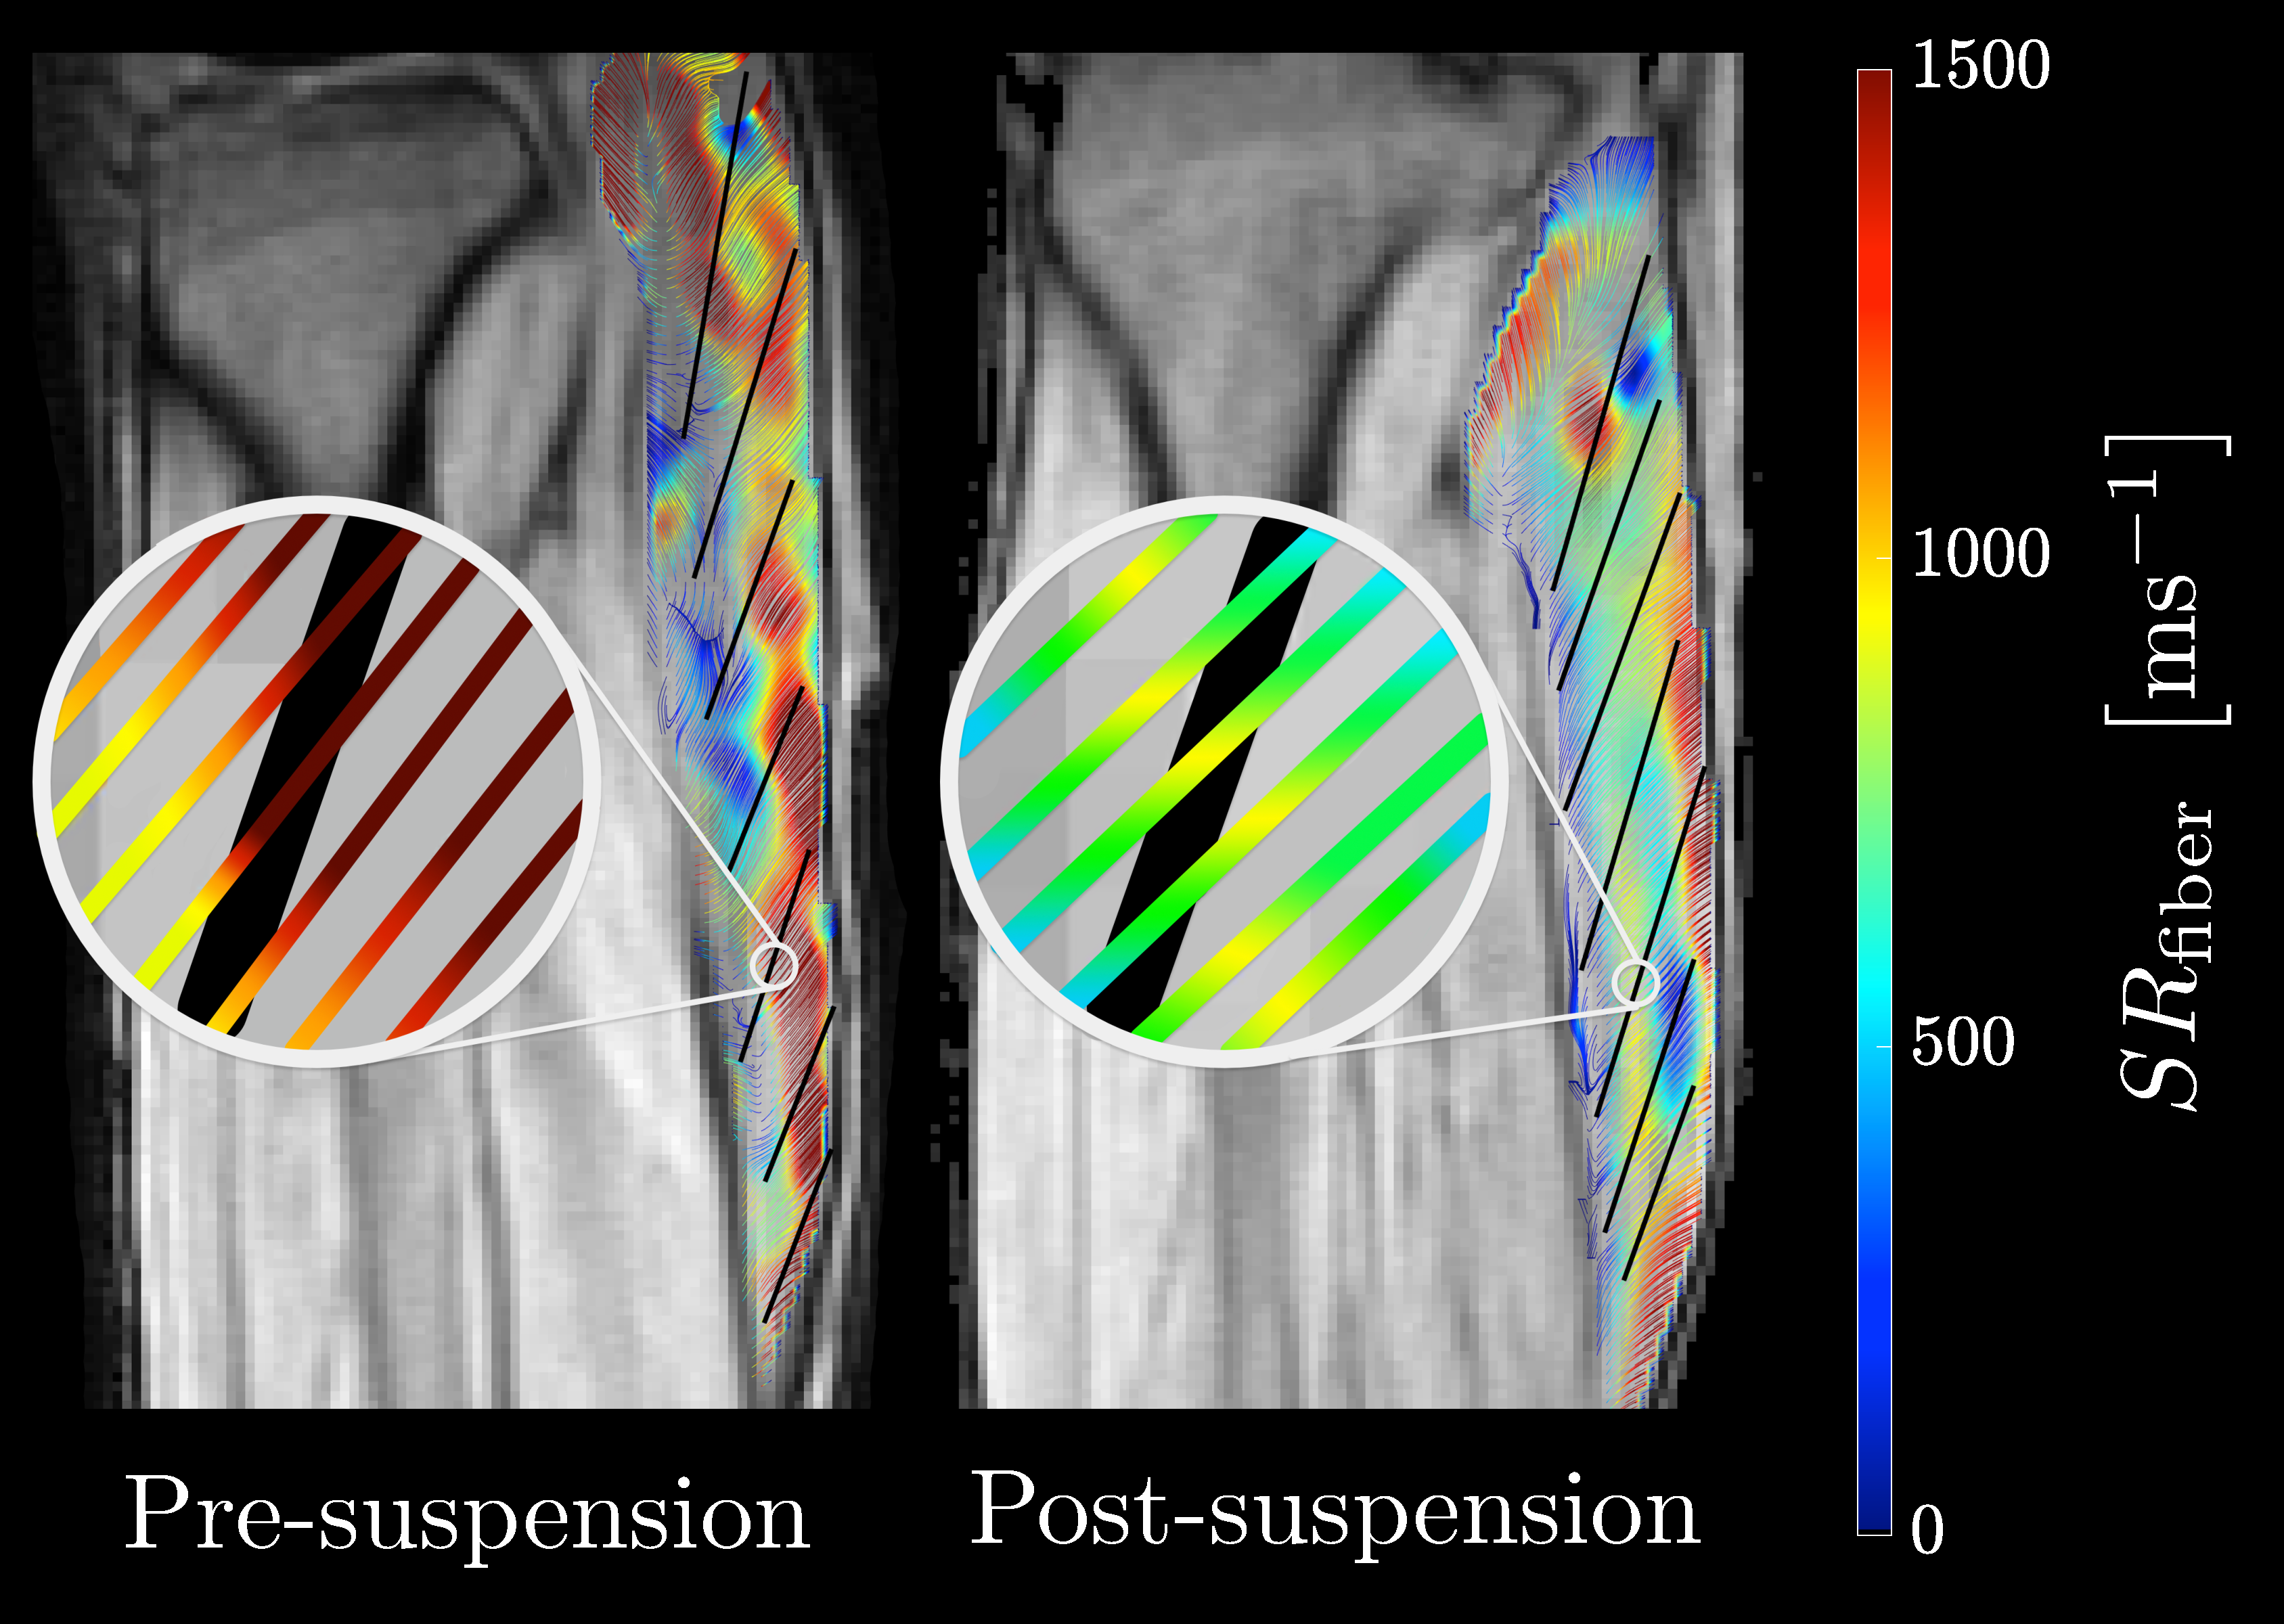
\includegraphics[width=0.9\textwidth]{Figures/ULLS_Streamlines.pdf}
%\captionsetup{width=8in}
\caption[Streamlines of strain rate tensor negative eigenvectors for one slice of the same subject pre- and post-suspension at the peak of contraction phase]{Streamlines of eigenvectors corresponding to negative eigenvalues (NEV = $SR_\mathrm{fiber}$ during contraction) overlaid on fiber directions (in black) for one slice of the same subject pre- and post-suspension at the peak of contraction phase.}
\label{fig: SR1_5}
\end{figure}
%\end{sidewaysfigure}
%*********************************************************
 Figure~\ref{fig: SR1_6} and Figure~\ref{fig: SR1_4} are plots of the temporal variation of the strain rates in the fiber basis. 
 As in the principal axes basis, the largest changes are seen in the deformation rate in the fiber cross-section (plot of $SR_{cc}$ in Figure~\ref{fig: SR1_4}).
%-new paragraph-%

%-new paragraph-%
The values of the SR indices in the principal axes and in the fiber basis were extracted at the force value corresponding to the post-suspension value of each subject (a subject was compared between the pre- and post-suspension states at the (lower) force level of the post-suspension) (Table~\ref{tab: SR1_2}).
%*********************************************************
\begin{figure}[!htb]
\vspace{+0.2cm}
\centering
\includegraphics[width=\textwidth]{Figures/ULLS_SRff.pdf}
\caption[The temporal variation of the strain rate indices in the muscle fiber basis with isometric contractions for the pre- and post-suspension cohorts in three regions]{The temporal variation of the strain rate indices in the muscle fiber basis with isometric contractions for the pre- and post-suspension cohorts in three regions (proximal, middle and distal). The values shown in this plot are the average over all subjects pre-and post-suspension.}
\label{fig: SR1_4}
\end{figure}
%*********************************************************
$SR_{\mathrm{in-plane}}$ in the pre-ULLS was significantly larger than in the post-ULLS cohort ($F(1, 6) = 17.734$, $p = 0.006$).
Significant difference in $SR_{\mathrm{in-plane}}$ was also found between different muscle regions ($F(2,12)=12.090$, $p = 0.001$). 
Follow up post hoc tests revealed that $SR_{\mathrm{in-plane}}$ was larger in the distal compared to the proximal ($p = 0.029$) and middle regions ($p = 0.034$). 
SR-fiber angle was significantly larger post-ULLS ($F(1,6) = 9.435$, $p = 0.022$).
Significant time (pre, post)*region (proximal, middle, distal) interaction effects were found for $SR_{\mathrm{out-plane}}$ ($F(2, 12) = 8.484$, $p=0.005$). 
For the components of strain rate in fiber basis, a trend to significance was observed between pre and post-suspension in $SR_{cc}$ ($F(1,6) = 4.536$, $p=0.077$) which reflects the changes seen in $SR_{\mathrm{in-plane}}$ in the principal axes basis. 
Though normal and shear strain rates (fiber basis or maximum) decreased in the post-suspension subjects (Table~\ref{tab: SR1_2}) no significant differences were detected.
Significant regional differences were observed in the shear strain rate ($SR_{fc}$) ($F(2,12) = 19.924$, $p = 0.004$) with significantly larger shear strain rates in the distal ($p = 0.013$) and middle ($p = 0.009$) as compared to the proximal muscle region. 
Similar regional differences were seen in $SR_{fc\_\,\mathrm{max}}$ ($F(2,12) = 10.537$, $p = 0.012$) with significantly larger shear strain rates in the distal ($p = 0.041$) and middle ($p = 0.023$) compared to the proximal region. 
No significant interactions effects of time (pre-post)*region (proximal, middle, distal) were found.

The results of the univariate~/~multivariable regression analysis for force and for force changes are summarized in Tables~\ref{tab: SR1_3}~and ~\ref{tab: SR1_4}.
For the univariate analysis, the absolute value of $\beta$ refers to the correlation coefficient for a given predictor and a significant \textit{p-}value ($p < 0.05$) associated with a predictor indicates that the null hypothesis that beta is zero for that variable is rejected.
%=========================================================
\begin{landscape}
\centering
\begin{table}[!h]
\vspace{+0.2cm}
\caption[Strain rate indices for pre- and post-suspension computed at the same force level of the contraction phase]{Strain rate tensor components in the principal axis basis, in the muscle fiber basis and in the maximum shear strain basis for pre- and post-suspension computed at the same force level of the contraction phase.}
\label{tab: SR1_2}
\begin{center}
\begin{threeparttable}
\begin{tabular}{@{}lllrrr@{}}
\toprule[1pt]\midrule[0.3pt]
\multicolumn{2}{c}{\multirow{2}{*}{SR indices}} & \multirow{2}{*}{ULLS} & \multicolumn{3}{c}{region}                         \\ \cmidrule(lr){4-6} 
\multicolumn{2}{c}{}                             &                       & \multicolumn{1}{c}{proximal} & \multicolumn{1}{c}{middle} & \multicolumn{1}{c}{distal}        \\ \cmidrule(){1-6}
\multirow{2}{*}{$SR_{\mathrm{fiber}}$}           & \multirow{2}{*}{$\left[ \SI{}{\per\milli\second}\right]$} 		& Pre-  & $-448.48 \pm 219.93$ & $-478.67 \pm 228.88$  & $-496.81 \pm 212.96$ \\
                                                 &														 	 		& Post- & $-218.70 \pm 138.91$ & $-295.21 \pm 223.73$  & $-423.47 \pm 362.89$ \\ [6pt]
\multirow{2}{*}{$SR_{\mathrm{in-plane}}$\tnote{1,2,3}}  & \multirow{2}{*}{$\left[ \SI{}{\per\milli\second}\right]$} & Pre-  & $259.11  \pm 79.04$  & $377.76  \pm 114.69$  & $492.04 \pm 249.22$  \\
                                                 &  														 			& Post- & $120.36  \pm 77.36$  & $161.17  \pm 88.21$   & $177.66 \pm 63.40$   \\ [6pt]
\multirow{2}{*}{$SR_{\mathrm{out-plane}}$\tnote{4}}     & \multirow{2}{*}{$\left[ \SI{}{\per\milli\second}\right]$} & Pre-  & $189.37  \pm 201.99$ & $100.91  \pm 199.69$  & $4.77 \pm 205.97$    \\
                                                 &  														 			& Post- & $98.34   \pm 180.06$ & $134.03  \pm 245.76$  & $245.81 \pm 359.86$  \\ [6pt]
\multirow{2}{*}{SR-fiber angle\tnote{1}}         & \multirow{2}{*}{$\left[\SI{}{\degree}\right]$}	 			 	& Pre-  & $27.09   \pm 5.67$   & $27.14   \pm 7.93$    & $32.45 \pm 8.85$     \\
                                                 & 														 			& Post- & $45.3    \pm 18.19$  & $39.37   \pm 15.78$   & $44.58 \pm 13.37$    \\ [6pt]
\multirow{2}{*}{$SR_{ff}$}                       & \multirow{2}{*}{$\left[ \SI{}{\per\milli\second}\right]$}	 		& Pre-  & $-287.19 \pm 207.43$ & $-304.56 \pm 214.32$  & $-234.99 \pm 81.65$  \\
                                                 &  													     			& Post- & $-132.67 \pm 104.11$ & $-155.42 \pm 93.40$   & $-166.9 \pm 145.68$  \\ [6pt]
\multirow{2}{*}{$SR_{cc}$}                       & \multirow{2}{*}{$\left[ \SI{}{\per\milli\second}\right]$} 		& Pre-  & $112.56  \pm 86.14$  & $184.14  \pm 134.39$  & $192.76 \pm 187.55$  \\
                                                 &  														 			& Post- & $-0.39   \pm 147.18$ & $5.51    \pm 274.19$  & $-156.89 \pm 299.33$ \\ [6pt]
\multirow{2}{*}{$SR_{fc}$\tnote{2,5}}            & \multirow{2}{*}{$\left[ \SI{}{\per\milli\second}\right]$} 		& Pre-  & $148.81  \pm 145.57$ & $229.88  \pm 206.9$   & $294.36 \pm 237.35$  \\
                                                 &  														 			& Post- & $93.34   \pm 60.97$  & $187.99  \pm 126.94$  & $287.92 \pm 198.53$  \\ [6pt]
\multirow{2}{*}{$SR_{fc\_\,\mathrm{max}}$\tnote{2,5}}   & \multirow{2}{*}{$\left[ \SI{}{\per\milli\second}\right]$} & Pre-  & $-295.75  \pm 181.69$ & $-389.03  \pm 229.29$  & $-409.13 \pm 249.11$  \\
                                                 &  														 			& Post- & $-198.38  \pm 80.26$  & $-257.19  \pm 112.06$  & $-369.34 \pm 188.3$   \\ \midrule[0.3pt]\bottomrule[1pt]
\end{tabular}
\begin{tablenotes}[flushleft]\footnotesize
\item[1] significant difference between pre- and post-suspension
\item[2] significant difference between proximal and distal regions
\item[3] significant difference between middle and distal region
\item[4] significant interaction time*region
\item[5] significant difference between proximal and middle region
\end{tablenotes}
\end{threeparttable}
\end{center}
\vspace{-0.2cm}
\end{table}
\end{landscape}
%=========================================================
For multivariable analysis, the R value is the multiple correlation coefficient and is a measure of the quality of the prediction of force; the value of $0.844$ (Table~\ref{tab: SR1_3}) indicates a good level of prediction.
The beta values provide a relative weight of each predictor in the multivariable regression and a significant \textit{p-}value ($p < 0.05$) associated with a predictor indicates that the null hypothesis for that variable is rejected. 
Stepwise multivariable analysis selected $SR_{\mathrm{in-plane}}$, SR-fiber angle and $V_{\mathrm{MG}}$ as significant predictors of force ($R=0.844$, $F=31.257$, $p<0.001$)
Due to the small number of subjects for force change (7 subjects), the univariate analysis was not extended to multivariable analysis for prediction of force change. 
Univariate analysis identified the $SR_{\mathrm{fiber}}$ and maximum shear strain $(SR_{fc\_\,\mathrm{max}})$ as significantly associated with change in force with unloading (Table~\ref{tab: SR1_4}). 
%=========================================================
\begin{table}[!htb]
\vspace{+0.2cm}
\caption[Univariate and multivariable linear regression analysis of morphological and strain rate indices to the force output]{Univariate and multivariable linear regression analysis of morphological and strain rate indices to the force output (MVIC).}
\label{tab: SR1_3}
\begin{center}
\begin{tabular}{@{}lrrrrrr@{}}
\toprule[1pt]\midrule[0.3pt]
               && \multicolumn{2}{c}{Univariate} &  & \multicolumn{2}{c}{Multivariable} \\ \cmidrule(lr){3-4} \cmidrule(lr){6-7}
               && \multicolumn{1}{c}{$\beta$}     & \multicolumn{1}{c}{$p$}            &  & \multicolumn{1}{c}{$\beta$}       & \multicolumn{1}{c}{$p$}              \\ \midrule
$SR_{\mathrm{fiber}}$       & & $-0.124$    & 0.433              &  &            &                     \\ [2pt]
$SR_{\mathrm{in-plane}}$    & & 0.426     & 0.005              &  & 0.277      & 0.007               \\ [2pt]
$SR_{\mathrm{out-plane}}$   & & $-0.129$    & 0.222              &  &            &                     \\ [2pt]
SR-fiber angle 			   & & $-0.528$    & $<0.001$   &  & $-0.299$     & 0.004               \\ [2pt]
$SR_{fc\_\,\mathrm{max}}$  & & $-0.098$     & 0.537              &  &            &                     \\ [2pt]
$V_{\mathrm{MG}}$          & & 0.692     & $<0.001$   &  & 0.629       & $<0.001$    \\ [2pt]
$V_{\mathrm{LG}}$          & & 0.690     & $<0.001$   &  &            &                     \\ [2pt]
$V_{\mathrm{SOL}}$         & & 0.655     & $<0.001$   &  &            &                     \\ \midrule[0.3pt]\bottomrule[1pt]
\end{tabular}
\end{center}
\vspace{-0.2cm}
\end{table}
%=========================================================
%=========================================================
\begin{table}[!htb]
\vspace{+0.2cm}
\caption[Univariate linear regression analysis of changes in morphological and strain rate indices to the change in force output after unloading]{Univariate linear regression analysis of changes in morphological and strain rate indices to the change in force output (MVIC) after unloading.}
\label{tab: SR1_4}
\begin{center}
\begin{tabular}{@{}lrrr@{}}
\toprule[1pt]\midrule[0.3pt] 
               &  & \multicolumn{1}{c}{$\beta$}      & \multicolumn{1}{c}{$p$}            \\ \midrule
$SR_{\mathrm{fiber}}$ 	 &  & $-0.732$    & $<0.001$    \\ [2pt]
$SR_{\mathrm{in-plane}}$  &  & 0.468     & 0.032              \\ [2pt]
$SR_{\mathrm{out-plane}}$ &  & 0.582     & 0.006              \\ [2pt]
SR-fiber angle 			 &  & $-0.242$    & 0.290              \\ [2pt]
$SR_{fc\_\,\mathrm{max}}$&  & $-0.721$     & $<0.001$   \\ [2pt]
$V_{\mathrm{MG}}$        &  & 0.286     & 0.217              \\ [2pt]
$V_{\mathrm{LG}}$ 		 &  & 0.095     & 0.578              \\ [2pt]
$V_{\mathrm{SOL}}$		 &  & 0.384     & 0.085              \\ \midrule[0.3pt]\bottomrule[1pt]

\end{tabular}
\end{center}
\vspace{-0.2cm}
\end{table}
%=========================================================
%~~~~~~~~~~~~~~~~~~~~~~~~~~~~~~~~~~~~~~~~~~~~~~~~~~~~~~~~~
\subsection{Discussion and Conclusion}
%~~~~~~~~~~~~~~~~~~~~~~~~~~~~~~~~~~~~~~~~~~~~~~~~~~~~~~~~~
In this study, an exploratory analysis of indices derived from the SR tensor was performed to determine any limb suspension related changes with the anticipation that these indices can be related to ECM remodeling.
It is to be noted that all the SR analysis was conducted at the same force level for pre- and post-suspension (that corresponding to the post-suspension force) and hence it was not at the peak force for the pre-suspension data.
However this insured that comparisons were not biased by different force levels for the pre- and post-suspension data. 
Further, a loss of $\sim 30\%$ (from the suspension intervention) shifted the point from peak force close to the beginning of the plateau level so that the pre-suspension values were not acquired too early in the contraction cycle.
While not reported here, data was also analyzed at the peak force (corresponding to the peak in $SR_{\mathrm{fiber}}$ during the contraction phase of the isometric cycle) and showed the same trends and significant differences between pre- and post-intervention as analysis at the same force level. 
It should be noted that comparison at the peak force corresponds to analysis at the same \%MVIC in contrast to the same force. 
%-new paragraph-%

%-new paragraph-%
$SR_{\mathrm{fiber}}$ and $SR_{ff}$  are the normal strain rate in a direction closest to the muscle fiber in the two basis. 
Though the two strain rates decreased post-suspension, the differences were not significant (Table~\ref{tab: SR1_2}). 
This is in contrast to findings in the aging study where younger cohorts showed significantly higher strain rates than older cohorts at isometric contraction~\cite{RNS16}. 
One of the hypotheses advanced to explain the age related decrease in strain rate was an increase in muscle stiffness with age arising from the remodeling of the extracellular matrix. 
Computational models predict that a stiffer extracellular matrix will result in reduced fascicle strain as well as force output~\cite{RNS28}. 
It is likely that the extensive ECM remodeling with the aging atrophy model that results in increased stiffness of the matrix is not present in the disuse atrophy model investigated herein or the increase in stiffness in ECM may not be as pronounced. 
However, there is increasing evidence that changes in the ECM play an important role in disuse-muscle atrophy.
This is because disruption of muscle cell adhesion to the extracellular matrix leads to muscle wasting~\cite{RNS29, RNS30}.
 For instance, degeneration of basal membrane components by matrix metalloproteases (MMPs) and alterations in mRNA and protein for extracellular matrix components have been found in disuse-muscle atrophy~\cite{RNS29, RNS30}.
%-new paragraph-%

%-new paragraph-%
Significant decreases in $SR_{\mathrm{in-plane}}$ are seen post-suspension (Table~\ref{tab: SR1_2}). 
The changes in $SR_{\mathrm{in-plane}}$ reflect the changes in deformation asymmetry in the fiber cross-section. 
In general, the reduction in $SR_{\mathrm{in-plane}}$ indicates that asymmetry of deformation in the fiber cross-section is reduced post-suspension. 
While deformation asymmetry is most pronounced in the distal regions in both pre- and post-suspension, the axis of greater deformation changes from in-plane (pre) to out-plane (post) in the distal regions. 
Similar to $SR_{\mathrm{in-plane}}$, $SR_{cc}$ which is the in-plane deformation in the fiber basis, is reduced post-suspension with a trend to significance (Table~\ref{tab: SR1_2}).
Asymmetry in deformation in the fiber cross-section has been reported in prior studies~\cite{RNS16, RNS31, RNS32} and one hypothesis for asymmetric deformation is that constraints (to deformation) are introduced by a specific orientation of tensile material (e.g. costameres). 
Costameres can be described in simple terms as a protein assembly that anchors myofibrils to the sarcolemma and to the extracellular matrix, and thus acts as important bridge between the muscle's contractile and other structural components~\cite{RNS33}.
Prior studies using the ULLS model identified a large decrease in costameric proteins, such as focal adhesion kinase, which could potentially contribute to the disproportionate loss of muscle force ($30\%$) compared to the decrease in quadriceps muscle CSA ($\sim 5\%$)~\cite{RNS8, RNS17}.
This is because costameres provide the key functional role of adhesion between adjacent muscle fibers and between muscle fibers and the surrounding connective tissue~\cite{RNS34}.
An earlier modeling paper predicted that when there is a strongly anisotropic constraint (which was postulated to arise from a specific structural arrangement of costameres), the force output may increase by a factor of two~\cite{RNS28}.
Conversely, it is reasonable to speculate that when the anisotropy in stiffness decreases (implied by the decrease in asymmetry of deformation) it could account for the loss of force seen post-suspension. 
%-new paragraph-%

%-new paragraph-%
Regional differences in $SR_{\mathrm{in-plane}}$ eigenvalues were seen with distal regions showing the highest strain rates.
Spatial heterogeneity of $SR_{\mathrm{in-plane}}$ and $SR_{\mathrm{out-plane}}$ is related to the regional variation of the asymmetry of deformation in the fiber cross section. 
The increasing deformation asymmetry at the distal end in the pre-suspension cohort may be related to the fiber packing density along the muscle length that increases from proximal to distal regions.
Earlier studies have also reported regional heterogeneity in strain in the calf muscles~\cite{RNS24} and in the brachis plexus~\cite{RNS35}.
The reduced asymmetry even in distal regions for the post-suspension cohort (Table~\ref{tab: SR1_2}) could arise from a combination of fiber atrophy and from alterations in the ECM. 
%-new paragraph-%

%-new paragraph-%
The deviation (non-zero SR-fiber angle, Table~\ref{tab: SR1_2}) of the principle axis of contraction from the muscle fiber orientation is seen in both pre- and post-suspension and this angle increases significantly post-suspension. 
Deviation of the principal axis of strain from that of the fiber has been observed in other muscles such as the anterior tibialis~\cite{RNS31}, biceps brachii~\cite{RNS35} and the myocardium~\cite{RNS36} and this deviation has been attributed to shearing between muscle fibers~\cite{RNS37, RNS38}. 
The larger SR-fiber angle post-suspension may be related to an increase in $SR_{\mathrm{fiber}}$ heterogeneity (Table~\ref{tab: SR1_2} shows that $SR_{\mathrm{fiber}}$ values in distal regions is higher by $50\%$ compared to proximal regions in the post-suspension cohort; equivalent value in the pre-suspension data is $5\%$).
It is likely that in the post-suspension state, the much higher relative strain rates in the distal regions results in larger SR-fiber angles through the shearing of the endomysium.
%-new paragraph-%

%-new paragraph-%
Shear strain rates (schematic shown in Figure~\ref{fig: SR1_1}b) are related to SR-fiber angles and Equation~\ref{eq: SR shear} shows the relationship between the two variables (shear strain rate increases with the SR-fiber angle).
However, it can be seen from Table~\ref{tab: SR1_2} that shear strain rates $(SR_{fc}\text{ and }SR_{fc\_\,\mathrm{max}})$ calculated from the eigenvalues and SR-fiber angle decrease in all three regions post-suspension. 
This decrease $(\text{in }SR_{fc} \text{ and }SR_{fc\_\,\mathrm{max}})$ is essentially from the decrease in $SR_{\mathrm{fiber}}$ and in $SR_{\mathrm{in-plane}}$ values post-suspension. 
Computational models predict that, in the prematurely terminating fiber, shearing of the endomysium is the most likely pathway for lateral transmission of force produced by the non-spanning fibers~\cite{RNS15}.
The observed reduction in shear strain rate (in fiber basis or max shear strain basis) with suspension did not reach significance but it may be speculated that the changes in $SR_{fc}/SR_{fc\_\,\mathrm{max}}$ may translate to a reduction in lateral transmission of force. 
This reduction in LTF may then account for the loss in total force that is not explained by muscle atrophy, activation, and specific tension changes with unloading. 
%-new paragraph-%

%-new paragraph-%
The identification of $SR_{\mathrm{in-plane}}$, SR-fiber angle and $V_{\mathrm{MG}}$ in stepwise multivariable regression as significant predictors of force has interesting physiological implications. 
The volume of the MG muscle may reflect the size and number of muscle fibers as well as the extent of connective tissue as well as fatty infiltration. 
While aging has been shown to lead to increase in fatty infiltration as well as an increase in the width of connective tissue~\cite{RNS39}, preliminary results on suspension induced disuse atrophy from our group did not reveal a change in fat or connective tissue content.
Thus, it is plausible to infer that volume differences in the MG within the cohort of pre- and post- suspension subjects reflect the size and number of muscle fibers and since the size~/~number of muscle fibers determines contractility, it is anticipated to be a predictor of force.
The relationship of $SR_{\mathrm{in-plane}}$ and SR-fiber angle to force is more complex: $SR_{\mathrm{in-plane}}$ reflects the constraints (in the extracellular matrix) that modulate the extent of deformation in-plane that, as detailed earlier, may have an effect on the total force produced. 
SR-fiber angle is related to shear in the endomysium (Figure~\ref{fig: SR1_1}).
Since $SR_{\mathrm{in-plane}}$ and $SR_{\mathrm{fiber}}$ angle are parameters that are influenced by the ECM, their relationship to force highlights the role of the ECM in the force output.
In univariate analysis, the significant predictors of force change with unloading are the SR eigenvalues and $SR_{fc}/SR_{fc\_\,\mathrm{max}}$.
 $SR_{\mathrm{fiber}}$ is a measure of contractility in the fiber direction and a decrease in its magnitude is anticipated to correlate to force loss.  $SR_{\mathrm{in-plane}}$ and $SR_{\mathrm{out-plane}}$ reflect the deformation asymmetry in the fiber cross-section and are influenced by changes in the ECM. 
$SR_{fc}/SR_{fc\_\,\mathrm{max}}$, the shear strain rate is also influenced by ECM remodeling and further, is postulated as the mechanism of lateral transmission of force; a decrease in the shear strain rate may potentially reduce lateral transmission of force (LTF). 
While changes in the ECM with unloading have been reported in prior studies~\cite{RNS13} and it has been postulated that this remodeling may result in modulating the lateral force transmission pathway leading to a loss of force output~\cite{RNIRamaswamy}, this is the first study to show that force changes (\textit{in-vivo} and in human subjects) on uploading are related to changes in shear strain. 
It should be noted that there are other determinants that will also contribute to force loss with unloading but in this exploratory work on a small cohort, the intent was to extract the contributions of the strain rates in the MG and morphological parameters of the plantarflexors to changes in force production. 
%-new paragraph-%

%-new paragraph-%
The limitations of this study are as follows. 
The number of subjects is small; however this was still sufficient to find significant differences in some of the SR indices during isometric contraction between the pre- and post-suspension cohorts and to detect significant regional differences. 
Muscle fiber and its direction were indirectly determined and the accuracy of the fiber orientation depends on the accuracy of locating fascicles in the magnitude images. 
On the other hand, diffusion tensor imaging provides fiber directions directly. 
However, it should be noted that the method used in the current study is the only way to track muscle fibers over a large region of interest through the dynamic cycle. 
Finally, noise in the imaging data can cause error propagation in the calculated indices especially as the computation involves the gradients of images that cause noise to be amplified.
%-new paragraph-%

%-new paragraph-%
The study confirms the overarching hypothesis that some of the indices derived from the strain rate tensor will show significant changes after unloading and that force loss in disuse atrophy will be predicted by SR parameters that are known to be influenced by the ECM remodeling. 
The two indices that showed significant changes were $SR_{\mathrm{in-plane}}$ and the SR-fiber angle; both these parameters are influenced by the ECM. Further, $SR_{\mathrm{in-plane}}$, SR-fiber angle, and VOLMG were identified from a multivariable regression analysis as predictors of force. $SR_{\mathrm{fiber}}$, $SR_{\mathrm{in-plane}}$, $SR_{\mathrm{out-plane}}$, $SR_{fc}/SR_{fc\_\,\mathrm{max}}$ were significant predictors of force change in univariate analysis.
$SR_{fc}/SR_{fc\_\,\mathrm{max}}$ reflects changes in ECM and importantly, the study shows that the shear strain rate (and potentially lateral transmission of force) is a predictor of force loss with atrophy.
The role of the ECM (and remodeling) is increasingly being identified in several musculoskeletal diseases states including muscular dystrophies, diabetes, and aging~\cite{RNS40}.
Lateral transmission of force may be impacted by changes in the ECM and techniques to non-invasively monitor ECM remodeling and its functional consequence may allow accurate diagnosis and tracking of these disease states, ability to tailor rehabilitative paradigms and to monitor the efficacy of drug interventions.
%=========================================================
\section {Shear Strain Rate From Velocity Encoded Phase-Contrast Imaging to Study Effects of Aging in Medial Gastrocnemius Muscle}
\label{sec: SR_SHEAR}
%=========================================================
The loss of muscle force that occurs with aging is disproportionately greater than the loss of muscle mass (atrophy) and is still not completely understood~\cite{RNSS6}.
Neural and contractile contributions to age related loss of muscle force have been explored extensively~\cite{RNS13}.
One potential determinant of age related loss of muscle force that has not been investigated in depth is the remodeling of the extracellular matrix (ECM) and its functional consequences~\cite{RNSS8}. 
Several studies have emphasized the importance of force transmission pathways: longitudinal transmission of force via the myotendinous junction and lateral transmission of force mediated by the extracellular matrix via myofascical pathways~\cite{RNSS8, RNIRamaswamy}.
Impairment in lateral transmission pathways with age have been demonstrated in aging rodents and has been linked to the remodeling of the ECM~\cite{RNIRamaswamy}. 
The shearing of the ECM has been postulated to be the underlying mechanism of lateral transmission of force; thus, measurement of the shear strain could potentially be a surrogate assessment of lateral transmission of force.
It should be emphasized, however, that the role of the ECM may not be limited to modulating the lateral transmission of force but it may be involved in a more general force transmission mechanism termed "myofascial force transmission"~\cite{RNSS4}.
%-new paragraph-%

%-new paragraph-%
This study extends an earlier work that explored the changes in muscle strain rate with age where the analysis was limited to normal strain rates in the principal basis~\cite{RNS16}.
The earlier study identified the strain rate components in the principal basis that significantly differed between young and old subjects. 
This study is focused on: ($i$) establishing the repeatability limits of strain rate components in human subjects, ($ii$) evaluating strain rate tensor components in the different bases to monitor age related differences in muscle deformation, and ($iii$) identifying the relationship between the SR parameters and muscle force in a cohort of young and senior subjects. 
The analysis was performed on the medial gastrocnemius under isometric contraction.
%~~~~~~~~~~~~~~~~~~~~~~~~~~~~~~~~~~~~~~~~~~~~~~~~~~~~~~~~~
\subsection{Methods}
%~~~~~~~~~~~~~~~~~~~~~~~~~~~~~~~~~~~~~~~~~~~~~~~~~~~~~~~~~
%---------------------------------------------------------
\subsubsection{Subjects}
%---------------------------------------------------------
The study was approved by the Medical Research Ethics Board of UC San Diego and conformed to the standards in the Declaration of Helsinki on the use of human subjects in research.
Six young ($26.1 \pm 2.3$ years old, height: $158.6 \pm \SI{5.6}{\centi\meter}$, mass: $50.8 \pm \SI{3.7}{\kilogram}$) and six senior ($76.7 \pm 8.3$ years old, height: $153.0 \pm \SI{2.0}{\centi\meter}$, mass: $57.4 \pm \SI{4.3}{\kilogram}$) healthy, moderately active, female subjects were included in this study after informed consent~\cite{RNS16}. 
Two subjects (one young: 25 years, one old: 65 years) were scanned on three separate days to determine the coefficient of variation (CV) and the repeatability coefficients (RC) of the SR components. 
%---------------------------------------------------------
\subsubsection{MR imaging}
%---------------------------------------------------------
MR imaging was performed on a $\SI{1.5}{\tesla}$ Signa HDx MR scanner (GE Medical Systems, WI, USA) using same protocol as described in section~\ref{sec: SR_ULLS}. 
Images were acquired during sub-maximal, isometric plantarflexion contraction at $35\%$ of the individual maximum voluntary isometric contraction (MVIC); this level was chosen so that all subjects could comply with the imaging protocol (72 contractions~/~cycle). 
MR imaging included high-resolution water saturated oblique sagittal fast spin echo (FSE) images of the medial gastrocnemius (MG) where muscle tissue (water) signal is suppressed while the fascicles (fat) appear hyperintense. 
The slice (oblique sagittal) that best depicted the fascicles was selected for the Velocity Encoded Phase-Contrast (VEPC) scan~\cite{RNS16}.
Subjects were provided real-time visual feedback of the force generated superposed on the target force curve to facilitate consistent contractions.
%---------------------------------------------------------
\subsubsection{Force measurements}
%---------------------------------------------------------
MVIC was determined for each subject as the best of three trials recorded prior to MRI~\cite{RNS16, RNSS10}. 
Torques were recorded during acquisition at a sampling frequency of $\SI{200}{\hertz}$.
Muscle force was computed by dividing the measured torque by the Achilles tendon moment arm length.
%~~~~~~~~~~~~~~~~~~~~~~~~~~~~~~~~~~~~~~~~~~~~~~~~~~~~~~~~~
\subsection{Computation of the Strain Rate Tensor }
%~~~~~~~~~~~~~~~~~~~~~~~~~~~~~~~~~~~~~~~~~~~~~~~~~~~~~~~~~
%---------------------------------------------------------
\subsubsection{Strain rate (SR) calculation in the principal basis}
%---------------------------------------------------------
The ($2 \times 2$) SR tensor was calculated from the spatial gradient of the velocity images (velocity validated using calibrated flow phantoms,~\cite{RNSS11}) and then diagonalized to obtain the eigenvalues ($SR_\mathrm{fiber}$, $SR_\mathrm{in-plane}$) and eigenvectors. 
$SR_\mathrm{fiber}$ denotes deformation in a direction closer to the muscle fiber axis (than the orthogonal SR component) and is negative during muscle fiber shortening and positive during relaxation. 
$SR_\mathrm{in-plane}$ denotes deformation in the muscle fiber cross-section and is positive during muscle fiber shortening and negative during relaxation. 
In this study, only a $2 \times 2$ SR tensor is computed since a single velocity encoded slice (selected such that the MG muscle fibers lie in the plane of the image) was acquired precluding the computation of the $z$-derivative of velocity required for the complete $3 \times 3$ tensor.
%---------------------------------------------------------
\subsubsection{Muscle fiber tracking}
%---------------------------------------------------------
Muscle fibers (end points on the aponeuroses) are located on the fast spin-echo images at the distal, middle and proximal regions, transferred to the first frame of the dynamic images and the end points are tracked through the isometric cycle~\cite{RNS16}.
%---------------------------------------------------------
\subsubsection{Strain rate in the fiber basis}
%---------------------------------------------------------
Strain rate in the fiber basis was computed by rotating the SR tensor in the principal axes frame to the fiber basis using the following rotational transformation:
%.........................................................
\begin{equation}\label{eq: SR2_1}
SR_{\mathrm{fb}}=\mathrm{R}\cdot SR_{\mathrm{pb}} \cdot \mathrm{R}^\intercal
\end{equation}
%.........................................................
%.........................................................
\begin{equation}\label{eq: SR2_2}
\mathrm{R} = \left [
\begin{matrix}
\cos{\theta} & -\sin{\theta}\\
\sin{\theta} & \cos{\theta}\\
\end{matrix} \right]
\end{equation}
%.........................................................
where $SR_{\mathrm{fb}}$ is the strain rate tensor in the fiber frame defined by the fiber axis, $f$, and the fiber in-plane cross-sectional axis, $c$; R is the 2D rotation matrix defined by the SR-fiber angle $\theta$ , and $SR_{\mathrm{pb}}$ is the strain rate tensor in the principal basis frame. 
$SR_{\mathrm{fb}}$ has diagonal elements $SR_{ff}$ and $SR_{cc}$ (normal strain along the fiber and in the cross-section respectively) and non-diagonal terms $SR_{fc}$ (shear strain) while $SR_{\mathrm{pb}}$ has the diagonal terms $SR_{\mathrm{fiber}}$ and $SR_{\mathrm{in-plane}}$ (negative and positive principal strain rates respectively) (Figure~\ref{fig: SR2_1}).
%*********************************************************
\begin{figure}[!htb]
\vspace{+0.2cm}
\centering
\includegraphics[scale=0.6]{Figures/SRYO_Schematic.pdf}
\caption[Schematic of a muscle fiber and endomysium with the principal basis and fiber basis]{Schematic of a muscle fiber and endomysium with the principal basis and fiber basis. The muscle fiber is shown contracting while the endomysium experiences a shear strain. The thick (unfilled) arrows show the lateral transmission of force pathways. Arrows indicate normal and shear strains.}
\label{fig: SR2_1}
\end{figure}
%*********************************************************
%---------------------------------------------------------
\subsubsection{Strain rate tensor in the maximum shear strain rate basis}
%--------------------------------------------------------
The maximum shear strain, $SR_{fc\_\,\mathrm{max}}$ was estimated by rotating $SR_{\mathrm{pb}}$ by $\SI{45}{\degree}$ (from tensor algebra, the maximum in the off-diagonal terms occurs $\SI{45}{\degree}$ from the principal axes~\cite{RNSS12}).
$SR_{\mathrm{fiber}}$, $SR_{\mathrm{in-plane}}$, $SR_{ff}$, and $SR_{cc}$ are called normal strains (defined as perpendicular to the face of an element and represented by the diagonal terms of the SR tensor) while $SR_{fc}$ and $SR_{fc\_\,\mathrm{max}}$ are shear strains (defined as parallel to face of an element and represented by off-diagonal terms in the SR tensor); the former is the shear strain in the muscle fiber basis and the latter is the maximum shear strain (Figure~\ref{fig: SR2_1}). 
Figure~\ref{fig: SR2_S1} shows the SR analysis pipeline and the anticipated variability in the computed SR components as a function of the variability in the velocity images.
%*********************************************************
\begin{figure}[!htb]
\vspace{+0.2cm}
\centering
\includegraphics[width=0.96\textwidth]{Figures/SRYO_error.pdf}
\caption[Pipeline of the strain rate analysis with associated uncertainties in the computed values]{Pipeline of the strain rate analysis to derive strain rate in the principal axes, muscle fiber basis and the maximum shear basis. It shows the uncertainty in the computed values as a function of the uncertainty in the (acquired) velocity data, $\delta v$.}
\label{fig: SR2_S1}
\end{figure}
%*********************************************************
%---------------------------------------------------------
\subsubsection{ROI measurements}
%---------------------------------------------------------
Regional analysis of normal and shear strains in the two bases was performed on regions of interest (ROIs) selected manually on the magnitude images at the proximal, middle, and distal regions (corresponding to distances at 75\%, 50\% and 25\% of the total muscle length from the distal end). 
Since the ROIs shifted with muscle motion, pixel tracking was performed to ensure that the same anatomical region was being sampled.
The SR indices were computed at two force levels: one at the peak force level for each subject and the other at a force level of the subject with the lowest maximum MVIC exerted by any subject. 
Peak values of the SR components were identified at the temporal frame of the negative eigenvalue peak ($SR_{\mathrm{fiber}}$) in the compression phase.
To extract values at the same force level for a subject, the temporal frame corresponding to the lowest MVIC (of all subjects) was located in the force-time curves and SR values were extracted from the closest frame of the dynamic MRI.
%---------------------------------------------------------
\subsubsection{Statistical analyses}
%---------------------------------------------------------
The coefficient of variation (CV) was calculated as the ratio of the within subject standard deviation, $S_w$, to the mean value expressed as a percentage (estimated from the three repeat measures). 
The repeatability coefficient, RC, which represents the threshold value below which the absolute differences between 2 measurements on the same subject is expected to lie for $95\%$ of the measurement pairs was calculated as ($0.0277*$mean$*$CV)~\cite{RNSS13}.
For all tests, the level of significance was set at $0.05$.
Univariate and stepwise multivariable linear regression was performed to identify predictors (MG strain rate parameters estimated at the peak of the SR) of force in a cohort of young and senior subjects.
The predictors tested were the strain parameters alone and did not include morphological parameters since the latter are already established as predictors; the focus here was to test if SR components were predictors and of these, to identify the most significant SR predictor(s)
For the multivariable analysis, only independent variables were retained.
The statistical analyses were carried out using SPSS (IBM Corporation, Chicago, IL).
%~~~~~~~~~~~~~~~~~~~~~~~~~~~~~~~~~~~~~~~~~~~~~~~~~~~~~~~~~
\subsection{Results}
%~~~~~~~~~~~~~~~~~~~~~~~~~~~~~~~~~~~~~~~~~~~~~~~~~~~~~~~~~
Muscle force was lower by 43\% in the senior cohort: young ($387 \pm \SI{43}{\newton}$) and senior ($220 \pm \SI{43}{\newton}$), $p < 0.05$.
This was accompanied by an 18\% lower volume of the triceps surae muscles of the senior cohort, implying that the entire force loss could not be accounted by a decrease in muscle volume. 
Figures~\ref{fig: SR2_2}~and~\ref{fig: SR2_3} show the colormaps of the normal strain rates in the principal basis ($SR_{\mathrm{fiber}}$, $SR_{\mathrm{in-plane}}$) and the maximum shear strain rate ($SR_{fc\_\,\mathrm{max}}$) for one young and one senior subject at the same force level (Figure~\ref{fig: SR2_2}) and at the peak force (Figure~\ref{fig: SR2_3}). 
%*********************************************************
\begin{figure}[!htb]
\vspace{+0.2cm}
\centering
\includegraphics[width=0.6\textwidth]{Figures/SRYO_SRColormaps1.pdf}
\caption[Strain rate maps of the normal and shear strain rates in a young and senior subject at the same force level]{Strain rate maps of the normal and shear strain rates in a young and senior subject at the same force level. Colormaps are overlaid on the magnitude image at the corresponding frame.}
\label{fig: SR2_2}
\end{figure}
%*********************************************************
%*********************************************************
\begin{figure}[!htb]
\vspace{+0.2cm}
\centering
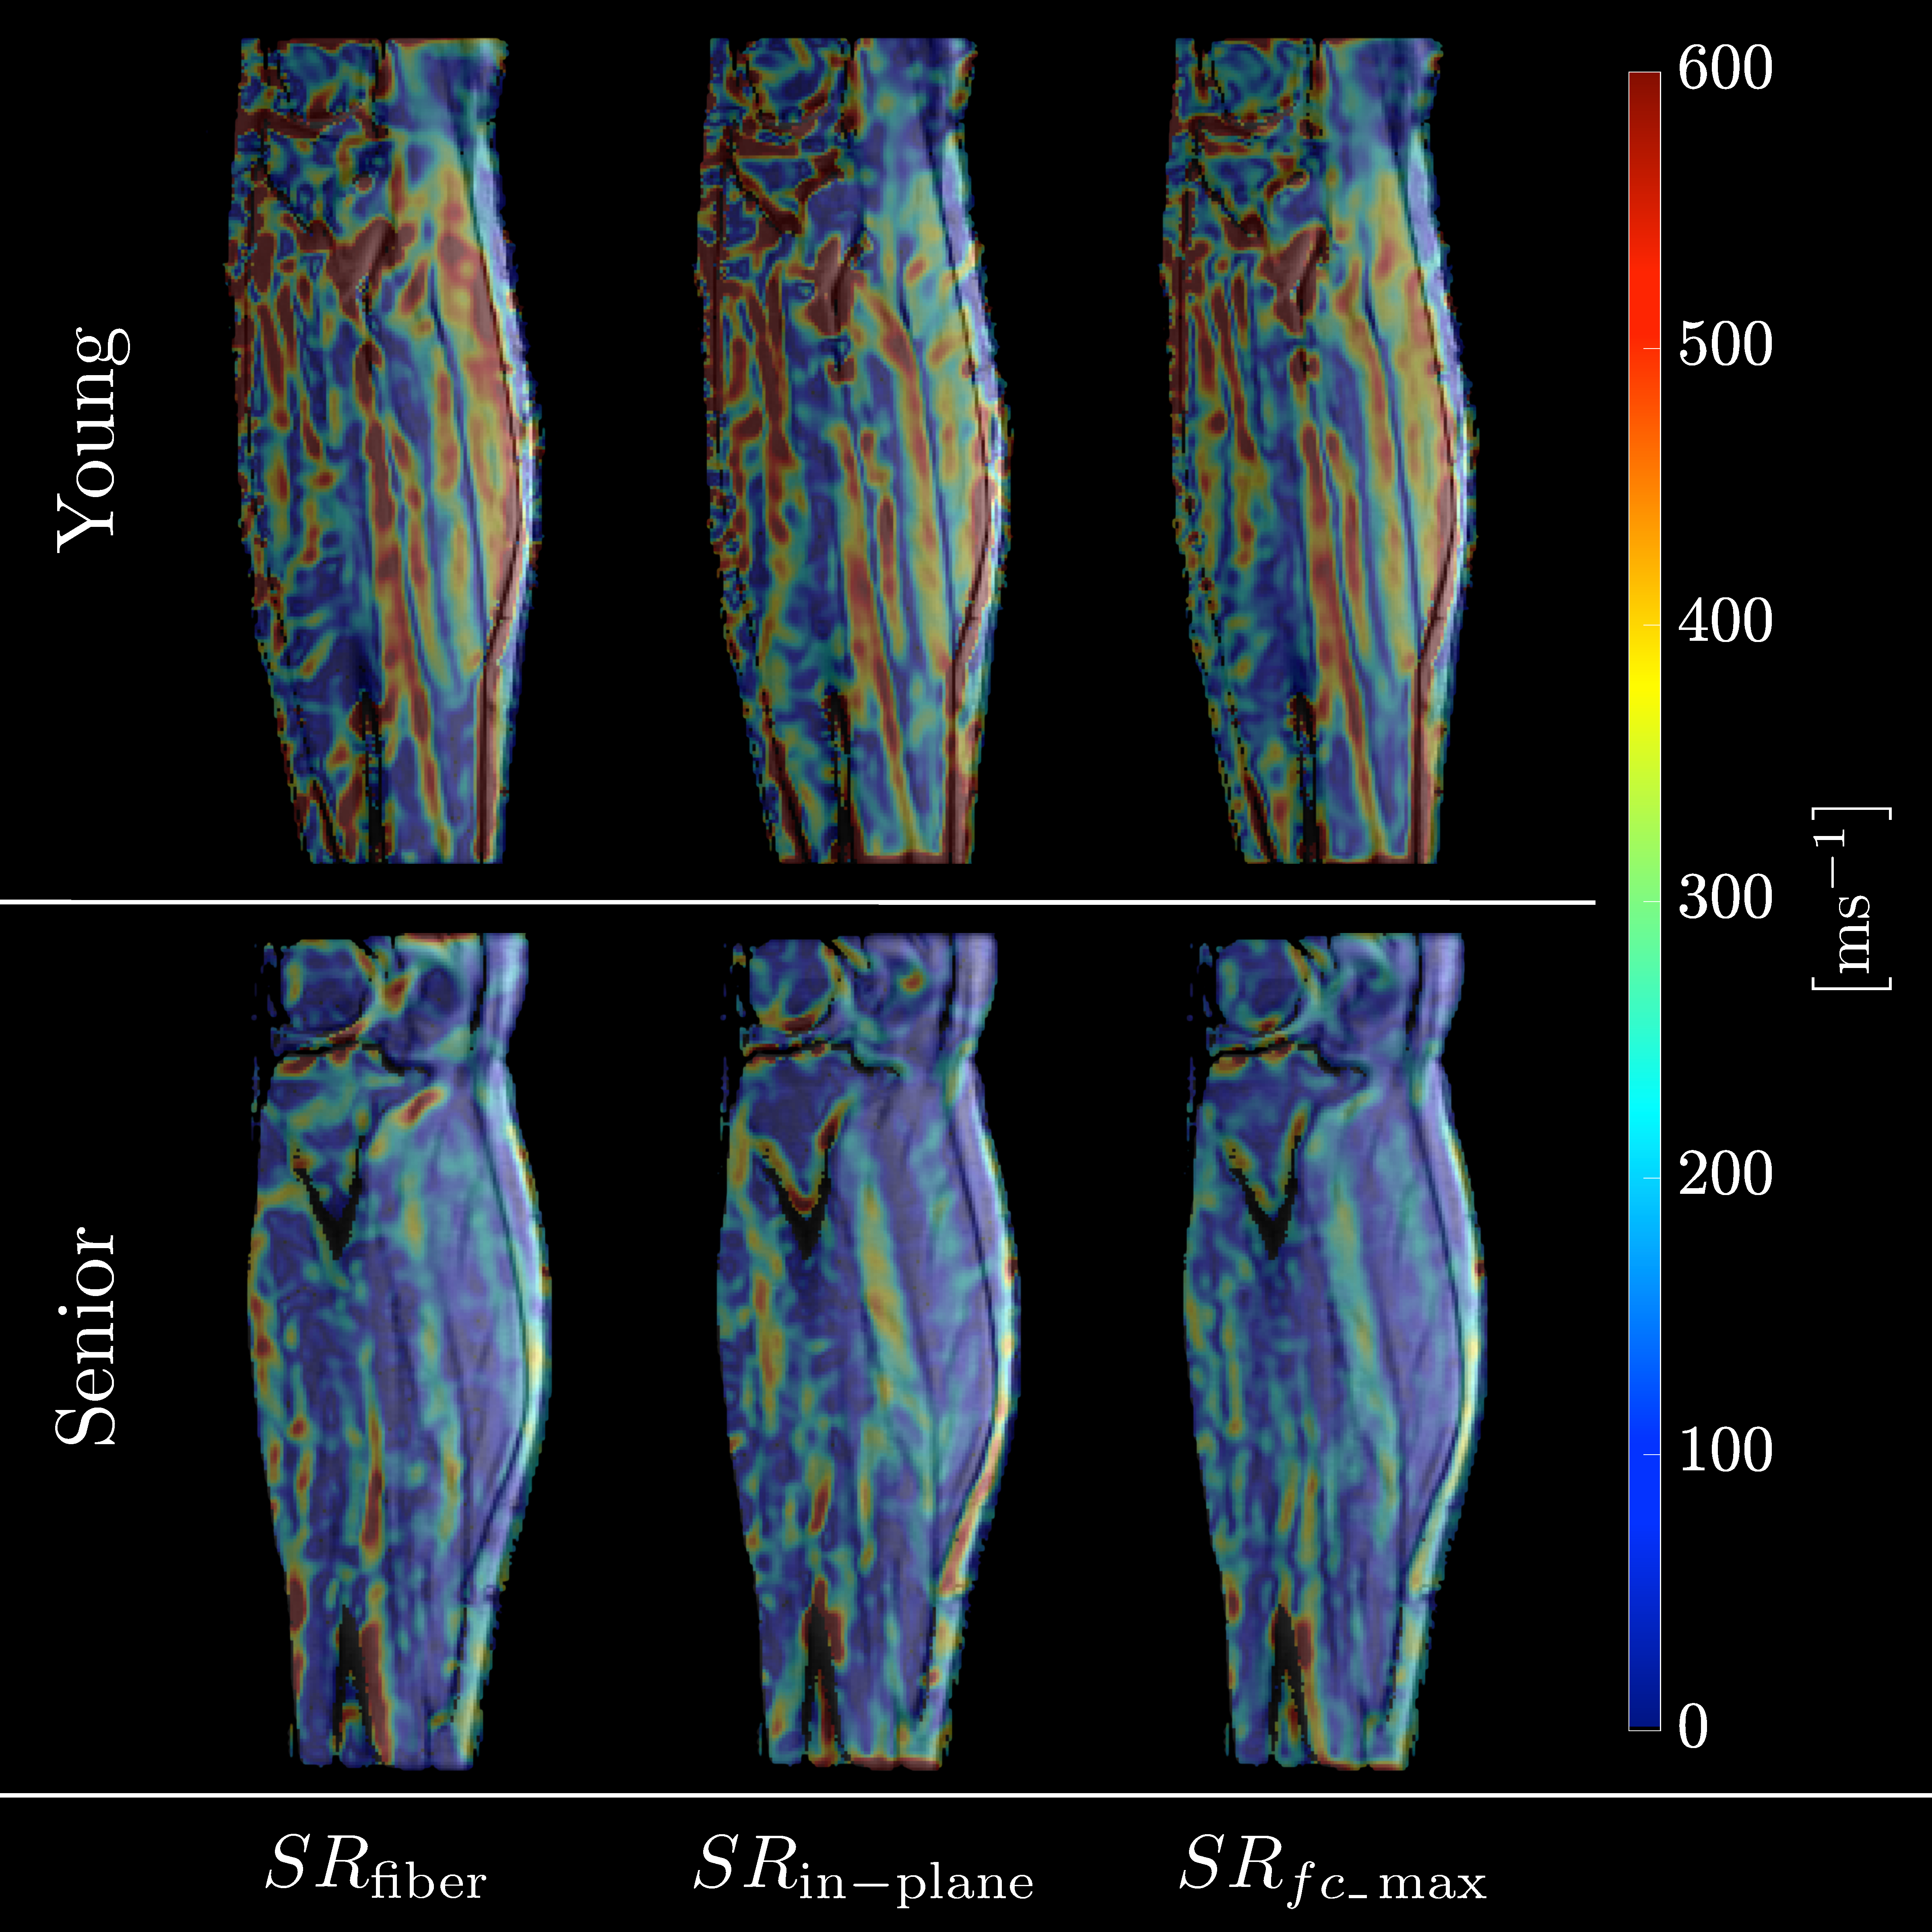
\includegraphics[width=0.6\textwidth]{Figures/SRYO_SRColormaps2.pdf}
\caption[Strain rate maps of the normal and shear strain rates in a young and senior subject at the peak force level]{Strain rate maps of the normal and shear strain rates in a young and senior subject at the peak force level. Colormaps are overlaid on the magnitude image at the corresponding frame.}
\label{fig: SR2_3}
\end{figure}
%*********************************************************
Figure~\ref{fig: SR2_S2} shows the temporal variation of the strain rate components as a function of the isometric contraction.
%*********************************************************
\begin{figure}[htb!]
\vspace{+0.2cm}
\centering
\includegraphics[width=0.9\textwidth]{Figures/SRYO_SRtemporal.pdf}
\caption[The temporal variation of the SR tensor indices with isometric contraction for the young and senior subjects]{The temporal variation of the SR tensor indices with isometric contraction for the young and senior subjects with isometric contraction. The values shown in this plot are the average over all subjects (young and senior separately).}
\label{fig: SR2_S2}
\end{figure}
%*********************************************************
Table~\ref{tab: SR2_1} lists the average values of the strain rate components for the young and senior cohorts at the same force level and at the peak of the force.
%=========================================================
\begin{table}[!htb]
\vspace{+0.2cm}
\caption[Strain rate indices for young and senior cohort at same force level and at peak force]{Strain rate indices for young and senior cohort averaged for three regions of interest in the principle, fiber, and maximum shear strain rate bases at same force level and at peak force.}
\label{tab: SR2_1}
\begin{center}
\begin{threeparttable}
\begin{tabular}{@{}llrrr@{}}
\toprule[1pt]\midrule[0.3pt]   
\multicolumn{2}{l}{Principle axis basis}	 	& $SR_\mathrm{fiber}$\tnote{$\dagger$} $\; \left[ \SI{}{\per\milli\second}\right]$ & $SR_\mathrm{in-plane}$\tnote{$\dagger$}   $\; \left[ \SI{}{\per\milli\second}\right]$ & $SR_{fc\_\,\mathrm{max}}$\tnote{$\dagger$}  $\; \left[ \SI{}{\per\milli\second}\right]$ \\ \midrule
\multicolumn{1}{l}{\multirow{3}{*}{Senior}} & same force level & $-245 \pm 192$  & 186 $\pm$ 120    & $-224$ $\pm$ 133  	\\
\multicolumn{1}{l}{}                        & peak             & $-280 \pm 196$  & 177 $\pm$ 102    & $-235$ $\pm$ 107  	\\
\multicolumn{1}{l}{}                        & CV, RC           & 3.9, 34.8   	 & 41.9, 222.8      & 9.3, 78.0  		\\ [6pt]
\multicolumn{1}{l}{\multirow{3}{*}{Young}}  & same force level & $-391 \pm 151$  & 280 $\pm$ 119    & $-335$ $\pm$ 107  	\\
\multicolumn{1}{l}{}                        & peak             & $-424 \pm 140$  & 298 $\pm$ 125    & $-351$ $\pm$ 108  	\\
\multicolumn{1}{l}{}                        & CV, RC           & 9.6, 135.5      & 23.5, 173.9      & 6.2, 58.5  		\\ \toprule[0.3pt]\midrule[0.3pt]
\multicolumn{2}{l}{Fiber basis}				& $SR_{ff}$   $\; \left[ \SI{}{\per\milli\second}\right]$     & $SR_{cc}$  $\; \left[ \SI{}{\per\milli\second}\right]$      & $SR_{fc}$  $\; \left[ \SI{}{\per\milli\second}\right]$      	\\ \midrule
\multicolumn{1}{l}{\multirow{2}{*}{Senior}}                     & same force level & $-170 \pm 118$  & 121.47 $\pm$ 134 & $-111$ $\pm$ 135  	\\
                                            & peak             & $-181 \pm 102$\tnote{$\dagger$} & 91 $\pm$ 173     & $-125$ $\pm$ 145  	\\ [6pt]
\multicolumn{1}{l}{\multirow{2}{*}{Young}}                      & same force level & $-259 \pm 146$  & 152 $\pm$ 146    & $-182$ $\pm$ 153  	\\
      	                                    & peak             & $-288 \pm 143$\tnote{$\dagger$} & 146 $\pm$ 168    & $-192$ $\pm$ 156  	\\ \midrule[0.3pt]\bottomrule[1pt]
\end{tabular}
\begin{tablenotes}[flushleft]\footnotesize
\item[$\dagger$] significant difference between age groups ($p<0.05$).
\end{tablenotes}
\end{threeparttable}
\end{center}
\vspace{-0.2cm}
\end{table}
%=========================================================
The mean value of all the regions (distal, middle and proximal) is reported since there was no regional variation in any of the SR parameters or any age*region interactions. 
CV and RC for $SR_{\mathrm{fiber}}$ and $SR_{fc\_\,\mathrm{max}}$ were $\sim 6\%$ and $\sim 17\%$ respectively; the RC value indicates that differences in these indices greater than 17\% between cohorts can be identified. 
However, the variability of $SR_{\mathrm{in-plane}}$ was much higher; this may potentially reflect the larger velocity uncertainties due to in-plane motion artifacts. 
%-new paragraph-%

%-new paragraph-%
Statistical analysis for the SR indices obtained at the same force and at peak force level showed significant age-related differences in: $SR_{\mathrm{fiber}}$, $SR_{\mathrm{in-plane}}$ and in $SR_{fc\_\,\mathrm{max}}$, and in addition, in $SR_{ff}$ for the peak force analysis alone. 
Tables~\ref{tab: SR2_2} and Tables~\ref{tab: SR2_3} summarize regression models for SR indices obtained at peak force level and at same force level respectively.
$SR_{ff}$ and $SR_{fc\_\,\mathrm{max}}$ (both negatively) were significantly correlated with force output, with $SR_{fc\_\,\mathrm{max}}$ having the strongest correlation. 
Stepwise multivariable regression produced a model with two predictors $SR_{fc\_\,\mathrm{max}}$, $SR_{cc}$ and with $R=0.681$ (moderately good level of prediction).
%=========================================================
\begin{table}[!htb]
\vspace{+0.2cm}
\caption[Univariate and multivariable linear regression analysis of parameters obtained at same force level with maximum volunteer isometric contraction]{Univariate and multivariable linear regression analysis of parameters obtained at same force level with a significant association with Maximum Volunteer Isometric Contraction (MVIC). Model ($R=0.640$, $F=11.448$, $p<0.001$).}
\label{tab: SR2_2}
\begin{center}
\begin{tabular}{@{}llrrrrr@{}}
\toprule[1pt]\midrule[0.3pt]
               && \multicolumn{2}{c}{Univariate} &  & \multicolumn{2}{c}{Multivariable} \\ \cmidrule(lr){3-4} \cmidrule(lr){6-7}
               && \multicolumn{1}{c}{$\beta$}     & \multicolumn{1}{c}{$p$}            &  & \multicolumn{1}{c}{$\beta$}       & \multicolumn{1}{c}{$p$}              \\ \midrule
$SR_{\mathrm{fiber}}$       & & $-0.421$   & 0.011              &  &            &                     \\ [2pt]
$SR_{\mathrm{in-plane}}$    & & 0.470    & 0.001              &  &            & 		                \\ [2pt]
$SR_{ff}$   				& & $-0.561$   & $<0.001$   &  &            &                     \\ [2pt]
$SR_{cc}$ 			   		& & 0.410    & 0.013				  &  & 	0.369	  &   0.012             \\ [2pt]
$SR_{fc}$  					& & $-0.339$   & 0.043              &  &            &                     \\ [2pt]
$SR_{fc\_\,\mathrm{max}}$   & & $-0.528$   & 0.001   			  &  &  $-0.606$    &   $<0.001$  \\ \midrule[0.3pt]\bottomrule[1pt]
\end{tabular}
\end{center}
\vspace{-0.2cm}
\end{table}
%=========================================================
%=========================================================
\begin{table}[!htb]
\vspace{+0.2cm}
\caption[Univariate and multivariable linear regression analysis of parameters obtained at force peak with maximum volunteer isometric contraction]{Univariate and multivariable linear regression analysis of parameters obtained at the peak of the contraction phase with a significant association with Maximum Volunteer Isometric Contraction (MVIC). Model ($R=0.681$, $F=14.034$, $p<0.001$).}
\label{tab: SR2_3}
\begin{center}
\begin{tabular}{@{}llrrrrr@{}}
\toprule[1pt]\midrule[0.3pt]
               && \multicolumn{2}{c}{Univariate} &  & \multicolumn{2}{c}{Multivariable} \\ \cmidrule(lr){3-4} \cmidrule(lr){6-7}
               && \multicolumn{1}{c}{$\beta$}     & \multicolumn{1}{c}{$p$}            &  & \multicolumn{1}{c}{$\beta$}       & \multicolumn{1}{c}{$p$}              \\ \midrule
$SR_{\mathrm{fiber}}$       & & $-0.353$   & 0.035              &  &            &                     \\ [2pt]
$SR_{\mathrm{in-plane}}$    & & 0.558    & $<0.001$   &  &            & 		                \\ [2pt]
$SR_{ff}$   				& & $-0.554$   & $<0.001$   &  &            &                     \\ [2pt]
$SR_{cc}$ 			   		& & 0.465    & 0.004			  	  &  & 	0.198	  &   0.009             \\ [2pt]
$SR_{fc}$  					& & $-0.262$   & 0.122              &  &            &                     \\ [2pt]
$SR_{fc\_\,\mathrm{max}}$   & & $-0.583$   & $<0.001$   &  &  $-0.393$    &   0.001  			\\ \midrule[0.3pt]\bottomrule[1pt]
\end{tabular}
\end{center}
\vspace{-0.2cm}
\end{table}
%=========================================================
%
%
%.  scatter plots... not needed   ...  overkill and not the best material to present
%
%Scatter plots of the univariate regression models for same force level and at peak force level are shown in Figure~\ref{fig: SR2_S3} and in Figure~\ref{fig: SR2_S4} respectively.
%*********************************************************
%\begin{figure}[!htb]
%\vspace{+0.2cm}
%\centering
%\includegraphics[width=\textwidth]{Figures/}
%\caption[Scatterplots of MVIC and the SR indices extracted at same force level]{Scatterplots of MVIC and the SR indices extracted at same force level.  Univariate linear regression fits for each SR parameter and the coefficient of determination ($R^2$) are provided for each index. $R^2$ values are low (max value of 0.315), however all six predictors are significant ($p<0.05$).}
%\label{fig: SR2_S3}
%\end{figure}
%*********************************************************
%*********************************************************
%\begin{figure}[!htb]
%\vspace{+0.2cm}
%\centering
%\includegraphics[width=\textwidth]{Figures/}
%\caption[Scatterplots of MVIC and the SR indices extracted at peak force]{Scatterplots of MVIC and the SR indices extracted at peak force. Univariate linear regression fits for each SR index and the coefficient of determination ($R^2$) are provided for each index. $R^2$ values are low (max value of 0.34), however five of the six predictors are significant ($p<0.05$).}
%\label{fig: SR2_S4}
%\end{figure}
%*********************************************************
%
%
%
%

%~~~~~~~~~~~~~~~~~~~~~~~~~~~~~~~~~~~~~~~~~~~~~~~~~~~~~~~~~
\subsection{Discussion}
%~~~~~~~~~~~~~~~~~~~~~~~~~~~~~~~~~~~~~~~~~~~~~~~~~~~~~~~~~
Examining the factors contributing to the variability in the measurements, the conclusion is that the primary sources arise from: inconsistency of the isometric, plantarflexion contractions, the intrinsic uncertainties in the SR measurement methodology, as well as from subject specific differences. 
Karakuzu~et~al. ecently noted that inter-individual differences in the muscle-tendon complex anatomy may in part be responsible for inter-subject strain variability~\cite{RNSS4}.
The first contribution to variability was minimized by the visual feedback.
Propagation of error analysis similar to that in~\cite{RNSS14} shows that the uncertainty in the SR is approximately eight times the uncertainty in the velocity.
This high variability is reflected in the ROI measurements though 2D anisotropic diffusion filtering of the velocity maps was performed to reduce the uncertainty in the velocity maps.
%-new paragraph-%

%-new paragraph-%
The results of the strain rate analysis in the principal basis and in the fiber basis show that normal strains along the fiber ($SR_{\mathrm{fiber}}$ and $SR_{ff}$) and in the fiber cross-section ($SR_{\mathrm{in-plane}}$) are significantly lower in the aging cohort. 
Azizi~et~al. showed by combining a mathematical model with experimental manipulation that the structural changes in the ECM (e.g., increase in collagen and in stiffness) compromise the muscle's ability to expand radially, which in turn restricts muscle shortening~\cite{RNSS15}. 
Thus, the observed changes in both the normal strains (along the fiber as well as in the fiber cross-section) can be explained, at least in part, to the structural changes in the ECM.  
Significant differences in the maximum shear strain rate were found between young and senior cohorts. 
The SR tensor including shear strain is measured at the voxel level precluding a direct assignment of the shear strain to the endomysium (very short $T_2$ and much smaller widths than MR voxel resolution).  
However, computational models have identified that endomysium (or ECM) shears and it is a reasonable extrapolation to associate the measured MR shear strain to the shear in the ECM.  T
his latter shear has been proposed to be the mechanism by which force is transmitted laterally~\cite{RNS15, RNSS17}. 
While a direct non-invasive measurement of lateral transmission of force (LTF) is not possible, the current analysis of shear strain rate may potentially be a surrogate measure of LTF. 
The ability to compute the shear strain rate, as reported in this paper, may provide a tool to explore, non-invasively and \textit{in-vivo}, modifications to lateral transmission pathways.
It is important to point out that a simplified model of a single muscle fiber and surrounding endomysium is considered here. 
In reality, when considering groups of active muscle, the situation is more complex and the shearing of the endomysium may potentially be attributed to the presence of complex intramuscular myofascial loads.  
Karakuzu~et~al. argue that epimuscular myofascial loads and intramuscular ones originating from the ECM and muscle fibers impact local deformations and are the underlying source of strain variability within a muscle~\cite{RNSS4}.
Their hypothesis of force transmission through the myofascial network is in agreement with the interpretation in this paper of the observed shear strain as potentially arising from the shearing of the endomysium.
It should be noted that the mechanical role of the ECM is not limited "lateral transmission of force".
Some of the findings observed in the current paper such as increased strain rates in the anterior compartment muscles of the triceps surae may be explained by a more general force transmission mechanism: "myofascial force transmission".
The latter force transmission pathway considers the skeletal muscle within a myofascial continuity, where ECM mechanically interacts with muscle fibers along their full lengths which are in turn, subject to further mechanical alterations through the surrounding muscles via epimuscular pathways~\cite{RNSS18}. 
Wilke~et~al. have recently shown that these mechanical interactions in turn have significant effects on the mechanical properties of the connective tissue~\cite{RNSS19}.  
It is highly likely that with age, the mechanical properties of the connective tissue (in the endomysium, perimysium and epimysium) are altered resulting in differences in strain rate components.
%-new paragraph-%

%-new paragraph-%
The current study shows that the basis frame in which the strain rate component is a maximum (principal basis for normal strains or shear strain maximum) is the most sensitive to detect age related changes (e.g., $SR_{\mathrm{fiber}}$, $SR_{\mathrm{in-plane}}$, $SR_{fc\_\,\mathrm{max}}$ show significant differences). 
Comparison at the same force level across all subjects makes the evaluation at a fairly low force level for most of the subjects and may not potentially be the optimum force level to detect changes. 
In contrast, evaluation at the peak of the force ensures the same effort level (\%MVIC) across subjects and further, is not limited by the force exerted by the weakest subject. 
Though significant differences in $SR_{\mathrm{fiber}}$, $SR_{\mathrm{in-plane}}$ and maximum shear strain rate were seen in evaluations by both methods, it may be physiologically meaningful to make the comparisons at the peak force level. 
In univariate analysis, several SR parameters were significantly correlated to force confirming that both normal and shear strain rates significantly predict muscle force output. 
It is also noteworthy that, in multivariable regression, the two significant predictors of force in a cohort of young and senior subjects are strain rate indices $SR_{cc}$ and $SR_{fc\_\,\mathrm{max}}$; both are known from other studies to be related to the status of the extracellular matrix~\cite{RNSS15, RNS15, RNSS17}.
%-new paragraph-%

%-new paragraph-%
It should be emphasized that the strain rate is in reality a $3 \times 3$ tensor, whereas only the $2 \times 2$ SR tensor is computed here.
The inability to compute the full $3 \times 3$ tensor arises from the fact that a single slice is acquired, which though encoded for velocity in three orthogonal directions does not allow the computations of the velocity gradient in the slice direction (thus precluding a $3 \times 3$ tensor analysis).  
In the protocol described here, multiple slices can be acquired in multiple scans but this will extend scan times such that senior subjects cannot tolerate. 
It is acknowledged that the identification of the fascicles as entirely in-plane (of the oblique sagittal slice in the current study) is not completely accurate as fascicles are known to be non-planar~\cite{RNSS20}.
In this context, it should be noted that the oblique sagittal slice for VEPC was identified following a specific protocol that resulted in the best depiction of the fascicles in the fast spin echo images. 
This protocol included ($i$) selecting the axial slice with the largest cross-section of the MG from a stack of axial slices of the calf muscle; ($ii$) positioning the oblique slice such that it bisected the distance between the femur and tibia and was perpendicular to it, and importantly; ($iii$) aligning the oblique slice with or parallel to the most prominent dark line depicting a fascicle in this axial slice. 
In the stack of such sagittal oblique "scout" slices, one of the slices generally had several prominent dark fascicular lines, which was subsequently used for the VEPC acquisition. 
Sometimes a second stack of scout slices had to acquired, to obtain the best depiction of the fascicles in the oblique sagittal planes (these "scout" scans were quite rapid). 
The accuracy of the orientation of the VEPC slice was ensured by checking for the most number and highest contrast of the dark fascicular lines in the oblique sagittal FSE images. 
The reproducibility of this slice orientation and position was confirmed after subject repositioning as part of the reproducibility studies. 
Ensuring the reproducibility of the orientation of the 2D VEPC slice is important, as the 2D tensor is sensitive to the orientation of the dynamic slice. 
While adherence to the above protocol ensured reproducible slice identification, accuracy of the slice orientation was also confirmed by examining the out-plane velocity values (sequence encodes velocity of the 2D oblique slice in all three directions). 
For the studies reported here, the out-plane velocity was negligible compared to the in-plane velocities. 
This is consistent with results from full 3D strain tensor studies where the strain in the out-plane direction is almost zero~\cite{RNS31}. 
If the orientation of the VEPC slice was not accurate, out-plane velocity values would not be small compared to the in-plane velocity values. 
While in the current study the slice orientation was reproducible and minimized out-plane motion, it is acknowledged that 3D SR tensor computed from 3D volume acquisition combined with three direction velocity-encoding will provide a more accurate representation of muscle deformation.
%~~~~~~~~~~~~~~~~~~~~~~~~~~~~~~~~~~~~~~~~~~~~~~~~~~~~~~~~~
\subsection{Conclusion}
%~~~~~~~~~~~~~~~~~~~~~~~~~~~~~~~~~~~~~~~~~~~~~~~~~~~~~~~~~
The study presented focuses on establishing the feasibility of shear strain mapping with application to aging muscle. 
The variability of the computed indices is high, but despite the variability, the computation of the $2 \times 2$ SR tensor as opposed to the full $3 \times 3$ SR tensor, and the small number of subjects, significance was reached in detecting age related differences. 
This is a first report of the significant differences in shear strain between young and old cohorts and its significance in accounting for age related force variability in the cohorts. 
In order to disambiguate potential sex based differences in age related muscle deformations, this preliminary study is limited to female subjects.  
The most important finding of this study is the association of muscle force output to shear strain rate (in addition to normal strain rate) confirming that lower values of the shear strain rate may also contribute to age related loss of muscle force. 
%~~~~~~~~~~~~~~~~~~~~~~~~~~~~~~~~~~~~~~~~~~~~~~~~~~~~~~~~~
\section{Acknowledgments}
%~~~~~~~~~~~~~~~~~~~~~~~~~~~~~~~~~~~~~~~~~~~~~~~~~~~~~~~~~
Section~\ref{sec: SR_ULLS} is a reprint of material, with minor edits as it appears in: V.~Malis, U.~Sinha, R.~Csapo, M.~Narici, and S.~Sinha, ``Relationship of changes in strain rate indices estimated from velocity-encoded MR imaging to loss of muscle force following disuse atrophy,'' \emph{Magn. Reson. Med.}, vol. 79, no. 2, pp. 912-922, Feb. 2018.
%-new paragraph-%

%-new paragraph-%
Section~\ref{sec: SR_SHEAR} is a reprint of material, with minor edits as it appears in: U.~Sinha, V.~Malis, R.~Csapo, M.~Narici, and S.~Sinha, ``Shear strain rate from phase contrast velocity encoded MRI: Application to study effects of aging in the medial gastrocnemius muscle,'' \emph{J. Magn. Reson. Imaging}, vol. 48, no. 5, pp. 1351-1357, Nov. 2018.
%-new paragraph-%

%-new paragraph-%
The author of the dissertation was the primary author of these papers.
%#########################################################
\chapter{Compressed Sensing Velocity Encoded Phase-Contrast Imaging}
%#########################################################
This chapter includes a brief introduction into theory of compressed sensing and provides the details of compressed sensing application to Velocity Encoded Phase-Contrast imaging (VEPC).
%=========================================================
\section{Compressed Sensing}
%=========================================================
One of the greatest challenge in MR imaging is long scan time, which is directly proportional to the number of samples collected in the Fourier domain (\textit{k-}space).
In recent years the theory of compressed sensing as well as the sampling and reconstruction framework was developed \cite{Donoho:2006cia, 2008ISPM...25...21C, Lustig:2007cua}.
%-new paragraph-%

%-new paragraph-%
Let $k(\omega)$ be the \mbox{\textit{k-}space} data collected and the inverse Fourier transform of $k(\omega)$ is a reconstructed image $a(t)$, $t = (t_1, ... t_d) \in \mathbb{Z}^d_N$
%.........................................................
\begin{equation}
	k(\omega) = \sum_t{a(t)e^{-2\pi i (\omega_1 t_1 + ... + \omega_d t_d)/N}}
\end{equation}
%.........................................................
Is it possible to recover the same image $a$ from $k(\omega)$, where $\omega = (\omega_1, ..., \omega_d) \in \Omega$ and $\#\Omega < N^d$~? The answer emerges from the fact that MR images meet two important conditions: ($i$) MR images are sparse in a certain domain and ($ii$) Fourier encoding is not coherent with these sparse transformations. 
%Therefore image can be recovered for the undersampled dataset by solving constrained optimization problem.
%~~~~~~~~~~~~~~~~~~~~~~~~~~~~~~~~~~~~~~~~~~~~~~~~~~~~~~~~~
\subsection{Data Sparsity and Undersampling}
%~~~~~~~~~~~~~~~~~~~~~~~~~~~~~~~~~~~~~~~~~~~~~~~~~~~~~~~~~
MR data in the image domain in general are not sparse, yet in another domains the sparsity can still be achieved. 
Consider the signal $\mathbf{a}(t)$ expanded in the orthonormal basis $\mathcal{W}=\left[\mathbf{w}_1 \dots \mathbf{w}_n\right]$, where $\mathbf{w_i}$ are row vectors:
%.........................................................
\begin{equation}\label{signal of interest}
\mathbf{a}(t) = \sum_{i=1}^n	x_i \mathbf{w}_i(t)
\end{equation}
%.........................................................
with $x_i$ being an inner product of $\mathbf{a}$ and $\mathbf{w}_i$. 
If signal $\mathbf{a}(t)$ is sparse it's possible to discard a certain number of coefficients in the expansion without significant loss of information. 
Thus sparsity can be quantified by the percentage of largest transformation coefficients preserved for the sufficiently good reconstruction. 
A more rigorous quantification would be to call the the signal $\mathbf{a}(t)$ $S$-sparse if it has at most $S$ nonzero elements. 
Undersampled acquisition thus will collect only a subset of $m \in M$ coefficients, where $M \subset N$:
%.........................................................
\begin{equation}
	k_j = \left< \mathbf{a}, \mathbf{s}_j \right>
\end{equation}
%.........................................................
here $\mathbf{s}_j$ is one of the $m$ rows of the sensing basis $\mathcal{S} = [\mathbf{s}_1 \dots \mathbf{s}_m]$. 
%-new paragraph-%

%-new paragraph-%
Many different sparsifying transformations can be applied, some of the most widely used are wavelet transform, discrete cosine transformation (DCT), finite difference and Gabor transform \cite{Baker:2016vs}. 
Example in Figure~\ref{WaveletCSExample} shows: magnitude MR image obtained using FGRE (Fast gradient echo) (a), its wavelet transform (b) and image obtained from top 2.5\% of the wavelet coefficients (c).
Image in Figure~\ref{WaveletCSExample}c is visually indistinguishable from image in Figure~\ref{WaveletCSExample}a thus by preserving only limited number of largest wavelet coefficients it's still possible to get a sufficiently good reconstructed image.
This approach works well when fully-sampled image is known beforehand (e.g. image compression).
In MRI experiment the image data are \textit{a priori} unknown, therefore an acquisition strategy must be adopted.
%*********************************************************
\begin{figure}[!htb]
\vspace{+0.2cm}
    \centering
    \includegraphics[width=0.9\textwidth]{Figures/CS2.pdf}
    \caption[MRI image reconstructed from top 2.5\% of its wavelet coefficients]{Magnitude FGRE image (a); wavelet transformation (b) and image reconstructed from 2.5\% of the largest wavelet coefficients (c).}
    \label{WaveletCSExample}
\end{figure}
%*********************************************************
\FloatBarrier
%~~~~~~~~~~~~~~~~~~~~~~~~~~~~~~~~~~~~~~~~~~~~~~~~~~~~~~~~~
\subsection{Incoherent Measurements and Random Sampling}
%~~~~~~~~~~~~~~~~~~~~~~~~~~~~~~~~~~~~~~~~~~~~~~~~~~~~~~~~~
Undersampled data can be represented as following:
%.........................................................
\begin{equation} \label{kspace_multicoil}
\mathbf{k} = \mathcal{A} \mathbf{x} + \sigma,
\end{equation}
%.........................................................
where $\mathcal{A} = \mathcal{S}\mathcal{W}$ is sensing matrix of size $m \times n$, $\mathbf{x}$ is a vector represented by the set of coefficients $x_i$ defined in Equation~\ref{signal of interest} and $\sigma$ is noise. 
The recovered signal $\mathbf{a}^\star$ is given by $\mathbf{a}^\star = \mathcal{W} \mathbf{x}^\star$, where  $\mathbf{x}^\star$ is the solution to the following convex minimization problem:
%.........................................................
\begin{equation} \label{COP}
\begin{aligned}
	\min_{\mathbf{z} \in \mathbb{R}^n} \quad &\norm{\mathbf{z}}_1 \\
	\text{subject to} \quad  &\norm{\mathcal{A} \mathbf{z}-\mathbf{k}}_2 < \epsilon,
\end{aligned}
\end{equation}
%.........................................................
here $\epsilon$ is a threshold parameter to control the fidelity of reconstructed data and is set to be below expected noise level $\sigma$, $\ell_1$ and $\ell_2$ -norms are defined for a vector $\mathbf{z}$ according to the Equation~\ref{L12Norm}:
%.........................................................
\begin{equation} \label{L12Norm}
\begin{aligned}
	\norm{\mathbf{z}}_1 & = \sum_{n=1}^{N}{|z_n|} \\
	\norm{\mathbf{z}}_2 & = \sqrt{\sum_{n=1}^{N}{|z_n|}^2}
\end{aligned}
\end{equation}
%.........................................................
Before discussing reconstruction procedure it's important to address the properties of the sensing matrix. 
Sensing matrix should maintain two important properties: $(i)$ incoherence and ($ii$) restricted isometry property (RIP) \cite{Candes:2005fx}.
%---------------------------------------------------------
\subsubsection{Incoherence}
%---------------------------------------------------------
For compressed sensing framework the incoherence of a sensing basis $\mathcal{S}$ and the sparsifying basis $\mathcal{W}$ is of a great importance. 
Coherence $\mu$ measures the maximum correlation between elements of $\mathcal{S}$ and $\mathcal{W}$ and is defined as:
%.........................................................
\begin{equation}
	\mu (\mathcal{S}\mathcal{W}) = \sqrt{n} \max_{1\leq p, q\leq n}{\left|\left<{s_p , w_q}\right>\right|}
\end{equation}
%.........................................................
since $\mathcal{S}$ and $\mathcal{W}$ are orthonormal lower and upper boundary for $\mu \in \left[1,\sqrt{n}\right]$. 
Suppose that $\mathbf{a}$ in basis $\mathcal{W}$ is $S$-sparse then if:
%.........................................................
 \begin{equation}
 	m\geq C \cdot \mu^2(\mathcal{S}\mathcal{W}) \cdot S \cdot \log{n}
 \end{equation}
%.........................................................
the reconstruction of the signal of interest is exact with overwhelming probability \cite{2007InvPr..23..969C}. 
Clearly this result implies that the smaller coherence leads to less number of samples required for reconstruction.
%---------------------------------------------------------
\subsubsection{Restricted isometry property}
%---------------------------------------------------------
Application of compressed sensing framework to experiment requires to consider two important issues. 
First sparsity of signal of interest is always approximate rather than exact and second is noise. 
These two issues are crucial for robustness of the reconstruction algorithm. As shown in~\cite{Candes:2006fb}, when sensing matrix $\mathcal{A}$ satisfies Restricted Isometry Property (RIP):
%.........................................................
\begin{equation}
	\left(1-\delta_S\right)\norm{\mathbf{x}}^2_2\leq\norm{\mathcal{A}\mathbf{x}}^2_2\leq\left(1+\delta_S\right)\norm{\mathbf{x}}^2_2, \quad 0 < \delta_S < 1
\end{equation}
%.........................................................
the reconstruction is accurate. In other words all subsets of S columns of sensing matrix $\mathcal{A}$ are nearly orthogonal, so $S$-sparse vectors $\mathbf{x}$ cannot be in the nullspace of $\mathcal{S}$. 
Suppose that sensing matrix $\mathcal{A}$ satisfies the RIP of order $2S$ with isometry constant $\delta_{2s} < \sqrt{2} -1$ then the solution $\mathbf{x}^\star$ of \ref{COP} obeys:
%.........................................................
\begin{equation}\label{Reconstruction error}
	\norm{\mathbf{x}-\mathbf{x}^\star}_2 \leq C_1 \frac{\norm{\mathbf{x}-\mathbf{x}_S}_1}{\sqrt{S}} + C_2 \epsilon
\end{equation}
%.........................................................
where $C_1$ and $C_2$ are constants, which are typically small, $\mathbf{x_S}$ is $\mathbf{x}$ with all $x_i$ except largest $S$ set to zero. 
Hence reconstruction error is limited by sum of noise-less term $C_1$ and term $C_2$ proportional to noise threshold parameter $\epsilon$.
Since obeying RIP guarantees robust reconstruction \cite{Candes:2006fb} it's important for sensing matrix $\mathcal{A}$ to satisfy RIP. 
It was demonstrated by Cand{\`e}~et~al.~\cite{2008ISPM...25...21C} that possible sampling schemes for sensing matrix are: sampling $m$ columns uniformly at random from $n$, i.i.d from normal distribution with mean 0 and variance $1/m$ and many other random sampling schemes satisfy RIP with high probability~if:
%.........................................................
\begin{equation}
	m\geq C \cdot S \log{\frac{n}{S}}
\end{equation}
%.........................................................
%-new paragraph-%

%-new paragraph-%
Figure~\ref{CS1} illustrates incoherence between wavelet and Fourier transformations for point spread function, here random \textit{k-}space undersampling results in incoherent interference in the wavelet domain. 
The interference spreads mostly within the wavelet coefficients of the same scale and orientation. 
%*********************************************************
\begin{figure}[!htb]
\vspace{+0.2cm}
    \centering
    \includegraphics[width=\textwidth]{Figures/CS1.pdf}
    \caption[Incoherence between wavelet and Fourier domains]{Incoherence between wavelet and Fourier domains.}
    \label{CS1}
\end{figure}
%*********************************************************
%~~~~~~~~~~~~~~~~~~~~~~~~~~~~~~~~~~~~~~~~~~~~~~~~~~~~~~~~~
\subsection{Solution to the Constrained Optimization Problem}
%~~~~~~~~~~~~~~~~~~~~~~~~~~~~~~~~~~~~~~~~~~~~~~~~~~~~~~~~~
Reconstruction process requires to solve the constrained optimization problem~(Equation~\ref{COP}). 
For the velocity encoded MR signal this problem can be restated as following:
%.........................................................
\begin{equation} \label{CS COP}
\begin{aligned}
	\min_{\mathbf{I}}  \quad &\norm{\mathcal{F}_t \, \mathbf{I}}_1 \\
	\text{subject to} \quad  &\norm{\mathcal{F}_s \, \mathbf{I}-\mathbf{k}}_2 < \epsilon,
\end{aligned}
\end{equation}
%.........................................................
where vector $\mathbf{I}$ is an image of interest, sparsifying transform $\mathcal{F}_t$ is temporal Fourier operator, $\mathcal{F}_s$ is spatial Fourier operator, and vector $\mathbf{k}$ is undersampled MR \mbox{\textit{k-}space} data. 
Development of efficient solution algorithms to problem stated in Equation~\ref{CS COP} has been a subject of the research for many years by now. 
Multiple computational approaches exist and some of the most known and widely used are: Convex Relaxation, Iterative Thresholding, Gradient Pursuit and other~\cite{Qaisar:2013ff}. Nonlinear conjugate gradient method is one of the possible choices.
%---------------------------------------------------------
\subsubsection{Nonlinear conjugate gradient method}
%---------------------------------------------------------
Due to presence of noise in vector $\mathbf{k}$ constrained optimization problem~\ref{CS COP} should be relaxed to the least squares problem \cite{Yin:2011ts}:
%.........................................................
\begin{equation} \label{CS UOP}
	\min_{\mathbf{I}} \quad \norm{\mathcal{F}_s \mathbf{I} - \mathbf{k}}_{2}^{2} + \lambda_1 \, {\norm{\mathcal{F}_t \mathbf{I}}}_1
\end{equation}
%.........................................................
where $\lambda_1$ is the Lagrangian multiplier of the constraint from the Equation~\ref{CS COP}, which controls the tradeoff between sparsity term ($\ell_1$-norm term) and image consistency ($\ell_2$-norm term). 
Nonlinear conjugate gradient method (NCG) allows to solve minimization problem (Equation~\ref{CS UOP}) numerically if gradient  of the cost function $f(\mathbf{I})$ defined by Equation~\ref{CS UOP} can be computed \cite{Lustig:2007cua}. 
The second term of the cost function is an $\ell_1$-norm defined as a sum of absolute values, its derivative is not defined at $I_i = 0$, therefore an approximation by a smooth function is necessary. 
The most computationally efficient choice is $\left| x \right| \approx \sqrt{x^2 + \mu}$ \cite{Ramirez:2014up}. 
The gradient of $f(\mathbf{I})$ is then approximated:
%.........................................................
\begin{equation}
	\nabla f(\mathbf{I}) =  2 \mathcal{F}_s^* \left(\mathcal{F}_s \, \mathbf{I}-\mathbf{k} \right) + \lambda \mathcal{F}_t^*\mathcal{U}^{-1}\mathcal{F}_t\mathbf{I}
\end{equation} where $\mathcal{U}$ is a diagonal matrix defined as following:
\begin{equation}
	\mathcal{U}=\DiagMat{\sqrt{(\mathcal{F}_t\mathbf{I})^*_i \, (\mathcal{F}_t\mathbf{I})_i + \mu }}
\end{equation}
%.........................................................
with smoothing parameter $\mu \in \left[ 10^{-15} , 10^{-6} \right]$ \cite{Lustig:2007cua}.
NCG method is summarized in the following outline:
%-new paragraph-%

%-new paragraph-%
\noindent \begin{samepage} \textbf{NCG outline} \\
%+++++++++++++++++++++++++++++++++++++++++++++++++++++++++++++++++++++++++++++++++++++++++++++++++++++++
\indent \qquad \qquad \textit{input:} \, $f(\mathbf{I})$ - cost function, $\alpha$, $\beta$ - line search parameters\\ 
\indent \qquad \qquad \textit{output:} $\mathbf{I}$ - reconstructed image\\
\noindent\rule{15cm}{0.4pt} \\
$n=0$ \quad $I_0 = 0$ 
\begin{itemize}
	%\renewcommand{\labelitemi}{\scriptsize$-$}
	\item Initial search direction: $g_0 = \nabla f(I_0)$; $\Delta I_0 = -g_0$
	\item Backtracking-Armijo line search: $\tau = 1$
		\begin{itemize}
			\item \textbf{while} \quad $f(I_0 + \tau \Delta I_0) \leq f(I_0) + \alpha \tau \cdot \Re(g^*_0 \Delta I_0)$ \, \textbf{do} \, $\tau = \beta \tau$ \quad ($\star$)
		\end{itemize}
	\item Update search direction:
		\begin{itemize}
			\item $I_1 = I_0 + \tau \Delta I_0$, $g_1 = \nabla f(I_1)$, $\gamma = \cfrac{\norm{g_1}^2_2}{\norm{g_0}^2_2}$
			\item $\Delta I_1 = -g_1 + \gamma \Delta I_0$
		\end{itemize}
	\item $n=1$ 
\end{itemize} \vspace{-3mm} \noindent\rule{15cm}{0.4pt} \\
%+++++++++++++++++++++++++++++++++++++++++++++++++++++++++++++++++++++++++++++++++++++++++++++++++++++++
\textbf{for} \quad $0<n<N$, where $n \in \mathbb{N}$, $N$ - maximum number of iterations \quad \textbf{do}
\begin{itemize}
	%\renewcommand{\labelitemi}{\scriptsize$-$}
	\item Backtracking-Armijo line search: 	$\tau = 1$
		\begin{itemize}
			\item \textbf{while} \quad $f(I_{n} + \tau \Delta I_{n}) \leq f(I_{n}) + \alpha \tau \cdot \Re(g^*_{n} \Delta I_{n})$  \, \textbf{do} \, $\tau = \beta \tau$ \quad ($\star\star$)
		\end{itemize}
	\item Update search direction:
		\begin{itemize}
			\item $I_n = I_{n-1} + \tau \Delta I_{n-1}$, $g_n = \nabla f(I_n)$, $\gamma = \cfrac{\norm{g_n}^2_2}{\norm{g_{n-1}}^2_2}$
			\item $\Delta I_n = -g_n + \gamma \Delta I_{n-1}$
		\end{itemize}
	\item $n=n+1$ 
\end{itemize}
\textbf{end} \\
\noindent\rule{15cm}{0.4pt}
\end{samepage}\\
\newpage

%+++++++++++++++++++++++++++++++++++++++++++++++++++++++++++++++++++++++++++++++++++++++++++++++++++++++
At each iteration Backtracking-Armijo line-search is used since general backtracking line search fails to prevent the step $\tau$ from getting too large relative to the decrease~in~$f$. 
The Armijo-Goldstein condition ($\star$  and $\star \star$ in NCG outline) has a second term on the right-hand side requiring the achieved reduction in $f$ to be at least a fixed fraction $\alpha$ of the reduction promised by the first term of the Taylor series of $f(I_n)$~\cite{Armijo:1966di}. 
Both parameters $\alpha$ and $\beta \in (0,1)$. 
Compared to conjugate gradient (CG) method where $f$ is quadratic NCG has a number of choices for $\gamma$ parameter~\cite{Hager:2006wp}. 
Two most popular  are Fletcher-Reevs (given above in the NCG outline) and Polak-Ribi\`ere. 
The Fletcher-Reeves method converges if the starting point is sufficiently close to the desired minimum, whereas the Polak-Ribi\`ere method can, in rare cases, cycle infinitely without converging~\cite{Shewchuk:1994uc}.
%=========================================================
\section{Application of Compressed Sensing Methods for Monitoring Skeletal Muscle Kinematics}
\label{sec: CS_paper}
%=========================================================
Magnetic Resonance imaging has been established as a viable technique to study muscle kinematics (including strain mapping)~\cite{RNS31, RNSS4, RNCS3, RNCS4, RNCS5}. 
Several studies have established the feasibility of the VEPC based MRI technique for monitoring muscle velocity and strain rate mapping during passive muscle motion and for different contraction modes (e.g., for isometric, concentric and eccentric contraction patterns)~\cite{RNCS3, RNCS4, RNCS5} as well applied it to study differences in aging and young muscle as well as pre- and post- unloading~\cite{RNS16, Malis:2018fr}. 
However, the limitation of the VEPC is the long scan time that requires execution of $\sim 75$ consistent contractions for dynamic imaging ($\sim \SI{2}{\minute}~\SI{40}{\second}$).
Several methods have been developed to maintain the consistency of contraction; e.g., by providing a visual feedback of the measured force superposed on the target force curve~\cite{RNS16, Malis:2018fr}. 
However, this still limits the force that can be maintained for the duration of the scan; this is usually set at 30-35\% Maximum Voluntary Isometric Contraction (MVIC) to enable $\sim 75$ consistent contractions. 
Studying muscle kinematics for several \%MVICs including higher \%MVICs may provide better insights into differences in muscle kinematics between normal and diseased (e.g., sarcopenia, disuse atrophy, dystrophy) conditions~\cite{RNS16, Malis:2018fr}. 
The long scan times also prevent acquisition of multiple slices to extract the full 3D strain or strain rate tensor. 
Further, in order to decrease scan times, views per segment (VPS) up to 4 are employed, but this limits the acquired temporal resolution of the scans. 
A faster VEPC sequence with improved temporal resolution could possibly expand the domain of exploration of muscle kinematics. 
%-new paragraph-%

%-new paragraph-%
Compressed sensing (CS) has been applied successfully and extensively in MRI to accelerate scan times~\cite{Lustig:2007cua}. 
CS allows for reconstruction of undersampled MRI data based on the concept that an image with a sparse representation in a known transform domain can be recovered (without artifacts) from randomly undersampled \mbox{\textit{k-}space} data using a non-linear reconstruction. 
The maximum acceleration (CS undersampling factor) will be determined by the image sparsity in the transform domain; the experimental observation is that the number of required samples is approximately $\sim 4$ times the number of non-zero coefficients in the transform domain. 
Various sparsifying transforms have been introduced such as wavelet, Principal Component Analysis (PCA) and Fourier Transform (FT)~\cite{Lustig:2007cua}. 
For 2D imaging, practical considerations limit the randomness to the phase encode direction ($k_y$) while for 3D acquisitions, random undersampling can be performed in the two phase-encode directions ($k_y$ and $k_z$) allowing for higher acceleration factors. 
Further, in 2D dynamic imaging as in 2D VEPC, researchers have exploited the fact that each temporal frame can have a different random phase encode pattern and a joint reconstruction of all temporal frames exploits the randomness in two axes ($k_y$\textit{-t}) allowing for higher acceleration factors compared to independent reconstructions of each temporal frame. 
$k_y$\textit{-t} CS reconstruction has also been integrated with multiple coil sensitivity profiles to perform a joint reconstruction of raw data from all the coils: this allows higher acceleration factors than CS without multiple coils that still yields images without significant artifacts. 
This latter technique, termed $k_y$\textit{-t} SPARSE SENSE to reflect the combination of multi-coil (parallel) imaging and CS techniques, has been applied to first-pass cardiac perfusion imaging as well as to studying cardiovascular and hepatoportal vascular dynamics~\cite{RNCS9, RNCS10}. 
However, the $k_y$\textit{-t} SPARSE SENSE technique has not been applied to imaging muscle kinematics. 
It should be noted that muscle velocities are much lower than that encountered in cardiac or portal and hepatic veins blood flow imaging ($venc = \SI{80}{\centi\meter/\second}$), so the velocity encoding gradients are much larger for the VEPC sequence to map muscle motion ($venc = \SI{10}{\centi\meter/\second}$). 
The larger velocity encoding gradients result in noisier images, so that integrating compressed sensing with VEPC sequences mapping lower velocities may pose additional challenges. 
One recent paper reported 4D VEPC integrated with compressed sensing applied to muscle dynamics~\cite{RNCS11}.
The latter paper performed 3D volume acquisition with undersampling in the $k_y$ and $k_z$ axes with 3-directional velocity encoding. 
In order to leverage the undersampling in the slice direction, a fairly high number of partitions is required (e.g. $\Rightarrow 32$) that results, for the best acceleration factor reported in the latter paper ($\sim \times 6.4$), in scan times of $\sim \SI{2}{\minute}~\SI{46}{\second}$. 
Admittedly, the optimum approach for 3D strain rate tensor computation is to acquire in 3D with 3 directional velocity encoding to cover the entire muscle. 
However, the long acquisition time of the 3D sequence even with ($\sim \times 6.4$) undersampling~\cite{RNCS11} limits its application with regards to the goal of the current work to reduce the acquisitions to less than a minute. 
Further, earlier experimental observation was~\cite{Malis:2018fr}, that with appropriate orientation of the acquisition slice in the plane of the muscle fibers (e.g., oblique sagittal for the medial gastrocnemius), 5 contiguous slices of $\SI{5}{\milli\meter}$ thickness allows the extraction of the 3D strain/strain rate (SR) tensor in 3 slices and this is sufficient to capture the spatial variation of the 3D strain tensor along the length of the muscle. 
%-new paragraph-%

%-new paragraph-%
The advantages of a faster VEPC sequence for muscle imaging is that it will allow scans to be completed with a shorter number of contraction cycles; this will expand the applicability to cohorts that are limited in their ability to sustain consistent contraction levels for a large number of repetitions. 
These cohorts include older subjects (normal and sarcopenic) and subjects with skeletal muscle disorders such as disuse atrophy dystrophy. 
Further, a short VEPC sequence will also enable acquisitions at higher \%MVIC (and at several \%MVIC) in contrast to current MRI based muscle kinematics studies limited to a single \%MVIC ($\sim 35$\%MVIC) achievable using traditional longer VEPC sequences~\cite{RNS16, Malis:2018fr}. 
Differences in muscle performance between normal and abnormal (sarcopenic, dystrophy, disuse atrophy) muscle function may be characterized better by investigating over a range of \%MVICs to explore force-strain patterns~\cite{RNCS12}. 
%-new paragraph-%

%-new paragraph-%
The objective of this study was to integrate compressed sensing and multi-coil methods with 2D VEPC imaging to decrease total scan time to less than a minute and implement this to study muscle kinematics. 
The new sequence was first validated with a constant flow phantom and velocity from the fully sampled and undersampled acquisitions (at different accelerations) were compared to reference flowmeter values. 
Calf muscle tissue motion (velocity and strain rate) under isometric contraction was monitored by the reference VEPC sequence and compared to the undersampled VEPC sequences for different acceleration factors (obtained by combinations of \mbox{CS\textit{-factor}} and views per segment).
%~~~~~~~~~~~~~~~~~~~~~~~~~~~~~~~~~~~~~~~~~~~~~~~~~~~~~~~~~
\subsection{Methods}
%~~~~~~~~~~~~~~~~~~~~~~~~~~~~~~~~~~~~~~~~~~~~~~~~~~~~~~~~~
%---------------------------------------------------------
\subsubsection{Velocity encoded phase-contrast pulse sequence}
%---------------------------------------------------------
The VEPC pulse sequence with 3 directional velocity encoding and the reference (without any velocity encoding) shown in Figure~\ref{fig: VEPC} was modified for random undersampling with a different random pattern along the $k_y$ direction at each temporal frame. 
The reference VEPC sequence was implemented with 4 views per segment that resulted in an acquired temporal resolution of $\SI{285}{\milli\second}$  ($\sim 8$ acquired frames for the contraction cycle duration of $\SI{2.3}{\second}$); this acquired data was then interpolated using view sharing to reconstruct 17 temporal frames. 
As part of this study, both CS acceleration factors and views per segment were modified to reduce scan time while maintaining/increasing the acquired temporal resolution.
%---------------------------------------------------------
\subsubsection{Compressed sensing}
%---------------------------------------------------------

%`````````````````````````````````````````````````````````
\textit{k-space undersampling:}
%`````````````````````````````````````````````````````````
Undersampling was performed along the $k_y$ direction with a different random pattern at each temporal frame. 
The undersampling along the $k_y$ was a random variable density pattern that yielded a dense sampling at the center of \mbox{\textit{k-}space}. 
The pattern was drawn from a probability density function (PDF) (Figure~\ref{fig: CS2}a) given by 10th order polynomial:
%.........................................................
\begin{equation}\label{eq: CS1}
\mathrm{PDF} = (1-|k|)^{10} + m
\end{equation}
%.........................................................
Here $k$ is the magnitude of $k_y$ with the maximum and minimum values of $k_y$ normalized to $+1$ and $-1$ respectively and $m$ is the sampling density computed by using an iterative bisection method, where the value in each iteration is divided successively by 2. 
%*********************************************************
\begin{figure}[!htb]
\vspace{+0.2cm}
\centering
\includegraphics[width=0.9\textwidth]{Figures/CS1_1.pdf}
\caption[The probability density function, two times undersampled pattern for selected temporal frames and combined phase encode/temporal frame undersampling pattern]{The PDF from which the random undersampled phase encode (PE) pattern is drawn (a); CS\textit{-factor} $\times 2$ undersampling pattern for selected temporal frames with different patterns for each: black indicates not acquired, white indicates the acquired PE line (b); combined phase encode/temporal frame undersampling pattern (c).}
\label{fig: CS2}
\end{figure}
%*********************************************************
This method ensured dense sampling at the center of $k_y$ with decreasing $k_y$ density toward the edges of $k_y$ space~\cite{RNCS10}. 
Dense sampling at the center has been established as providing better CS reconstructed images than uniform random undersampling~\cite{Lustig:2007cua, RNCS9}.
%-new paragraph-%

%-new paragraph-%
The undersampling pattern for each temporal frame of the dynamic series was an independent random pattern (Figures~\ref{fig: CS2}b~and~\ref{fig: CS2}c) selected as recommended by Lustig~\cite{Lustig:2007cua}. 
In brief, an impulse at the origin in a 1D image is Fourier transformed to give a constant image. 
This constant 1D image is undersampled by the chosen random pattern and then a 1D iFFT is performed to obtain the 1D image of the impulse. 
If no undersampling is performed, then the impulse is completely recovered while the undersampling results in side lobes which are quantified as the sum of the coefficients not including the origin (denoted as interference) in the 1D image reconstructed by undersampling. 
The undersampling pattern with the lowest value for the interference (from 100 iterations) was chosen in separate iterations for a temporal frame. 
Different combinations of compressed sensing acceleration factors (\mbox{CS\textit{-factor}}) and views per segment (VPS) were tested for both \textit{in-vitro} phantom as well as for \textit{in-vivo} calf muscle studies (Figure~\ref{fig: CS3}).
%*********************************************************
\begin{figure}[!htb]
\vspace{+0.2cm}
\centering
\includegraphics[width=0.9\textwidth]{Figures/CS1_2.pdf}
\caption[The $k_y$\textit{-t} SPARSE SENSE acquisition and reconstruction pipeline]{The $k_y$\textit{-t} SPARSE SENSE acquisition and reconstruction pipeline. Different sampling patterns and views per segment were tested to identify the highest acceleration factors that would still produce artifact free images after CS reconstruction. \mbox{\textit{k-}space} data was the input, the zero filled iFFT was the start point for the Temporal FFT.}
\label{fig: CS3}
\end{figure}
%*********************************************************
The undersampled patterns generated as detailed above were integrated into the velocity encoded FGRE sequence by modifying the proprietary pulse sequence (GE Medical Systems, version 15M4, WI, USA) using the EPIC programming environment. 
The undersampled mask for each temporal frame was read from an external file. 
The entire sequence was tested on the simulation platform as well as during run-time to verify that the undersampled patterns were correctly reproduced.

%`````````````````````````````````````````````````````````
\textit{Compressed sensing iterative reconstruction:}
%`````````````````````````````````````````````````````````
The flowchart for the iterative non-linear reconstruction algorithm is shown in Figure~\ref{fig: CS3} and follows the $k_y$\textit{-t} SPARSE SENSE method reported earlier~\cite{RNCS9, RNCS10, RNCS14}. 
Data was downloaded from the scanner as the complex \mbox{\textit{k-}space} data for each coil for each temporal frame. 
Data from the multiple channels was combined to form a self-calibrated coil sensitivity map $\mathbb{C}$. 
The coil sensitivity map is obtained by a temporal average over all the phases followed by an adaptive array combination~\cite{RNCS15}.
%-new paragraph-%

%-new paragraph-%
A two-stage process is used to reconstruct the image; the first stage uses the temporal Fourier transform as the sparsifying transform while the second stage uses the temporal PCA as the sparsifying transform (Figure~\ref{fig: CS3}). 
The starting point of the first stage (temporal FT as the sparsifying transform) is the sensitivity-weighted multicoil image combination of the zero-filled Fourier reconstruction of the undersampled data. 
A joint reconstruction is performed over all coils and all temporal frames. 
CS reconstruction minimizes the functional shown in Equation~\ref{eq: CS2}:
%.........................................................
\begin{equation}\label{eq: CS2}
f\left(\mathbf{I}\right) = \min_{\mathbf{I}} |{\mathcal{F}_{\mathrm{su}} \mathbb{C} \cdot \mathbf{I} - \mathbb{K}| _{2}^{2}} + \lambda_{\mathcal{F}/\mathcal{PCA}} |{\mathcal{W}_{\mathcal{F}/\mathcal{PCA}} \cdot \mathbf{I}}|_1
\end{equation}
%.........................................................
where $\mathbf{I}$ (current reconstructed image) and $\mathbb{K}$ (acquired undersampled \mbox{\textit{k-}space} data) are defined according to Equations~\ref{eq: CS3}~and~\ref{eq: CS4} respectively:
%.........................................................
\begin{equation}\label{eq: CS3}
\mathbf{I} = \begin{bmatrix} 
    \mathbf{i}_{11} & \dots & \mathbf{i}_{t1} \\
    \vdots & \ddots & \\
    \mathbf{i}_{1N} &        & \mathbf{i}_{tN} 
    \end{bmatrix}
\end{equation}
%.........................................................
%.........................................................
\begin{equation}\label{eq: CS4}
    \mathbb{K} =\mathcal{F}_{\mathrm{su}} \mathbb{C} \cdot \mathbf{I} = \begin{bmatrix} 
    \mathbf{k}_{11} & \dots & \mathbf{k}_{t1} \\
    \vdots & \ddots & \\
    \mathbf{k}_{1N} &        & \mathbf{k}_{tN} 
    \end{bmatrix}
\end{equation}
%.........................................................
with $N$ being the number of coils and $t$, the number of temporal frames and $\mathcal{F}_{\mathrm{su}}$ and $\mathbb{C}$ are the spatially undersampled Fourier operator and coil sensitivity vector respectively defined by Equations~\ref{eq: CS5}:
%.........................................................
\begin{equation}\label{eq: CS5}
    \mathcal{F}_{\mathrm{su}} = \begin{bmatrix} 
    \mathrm{F_{su}}^{1} \\
    \vdots \\
    \mathrm{F_{su}}^{t}
    \end{bmatrix} , \quad \mathbb{C} = \left[ \mathrm{C}_1 \dots \mathrm{C}_N \right]
\end{equation}
%.........................................................
The functional in Equation~\ref{eq: CS1} was minimized using a nonlinear conjugate gradient method~\cite{Lustig:2007cua}. 
The $\ell_1$ norm term (second term on LHS) maximizes the sparsity in the transform domain, $\mathcal{W}_{\mathcal{F}/\mathcal{PCA}}$ is the sparsifying transform (temporal FT in the first stage and PCA in the second stage of CS reconstruction), the $\ell_2$ norm (first term on LHS) ensures data fidelity between the estimated image and the acquired data, and $\lambda_{\mathcal{F}/\mathcal{PCA}}$ is the regularization parameter whose value controls the balance between image sparsity and image fidelity.
%-new paragraph-%

%-new paragraph-%
The CS reconstruction was performed offline using in-house built software developed in MATLAB (version R2018b. The MathWorks Inc. MA, USA) running on macOS (version 10.14.5 Apple Inc. CA, USA). 
Using a computer with Intel Core i5 CPU at $\SI{3.5}{\giga\hertz}$ with $\SI{16}{\gibi\byte}$ global memory, the total computational time was $\sim \SI{30}{\minute}$ for each series.
%-new paragraph-%

%-new paragraph-%
%`````````````````````````````````````````````````````````
\textit{Optimization:}
%`````````````````````````````````````````````````````````
 The regularization parameters $\lambda$ and the number of iterations for the temporal FT and for the temporal PCA of the CS reconstruction were optimized independently for the flow phantom data and for the muscle data. 
 The acquired undersampled images were used for phantom optimization while simulated undersampled images were used in the muscle data optimization. 
 The latter choice was based on the fact that comparing the reference to the acquired undersampled images may be biased by small differences in the contraction patterns in two separate acquisitions. 
 Optimization was performed to minimize the Root Mean Square Error (RMSE) in velocity estimated from the difference between the velocity from the full \mbox{\textit{k-}space} and from the undersampled \mbox{\textit{k-}space} data. 
 For the phantom, the velocity was estimated in the three flow tubes while for the muscle data, the velocity was estimated in a region of interest (ROI) [20 pixels $\times$ 7 pixels $= \SI{23}{\milli\meter} \times \SI{8}{\milli\meter}$] placed in the medial gastrocnemius. 
 The optimization was performed for each CS acceleration factor stepping through a grid of values for $\lambda$ and the number of iterations in the following range: 
%.........................................................
\begin{align}\label{eq: CS6}
\lambda_{\mathcal{F}} = \left[ 0.01, 0.10\right], \Delta_{\lambda} = 5\times10^{-3} \qquad & \mathcal{F}_\text{ite} = [10;30], \Delta_{\text{ite}}=5 \\
\lambda_{\mathcal{PCA}} = \left[ 0, 0.10\right], \Delta_{\lambda} = 5\times10^{-3} \qquad & \mathcal{PCA}_\text{ite} = [10;30], \Delta_{\text{ite}}=5 
\end{align}
%.........................................................
%---------------------------------------------------------
\subsubsection{Static and flow phantom}
%---------------------------------------------------------
Three tubes (diameter of 1cm) with constant flow were wound around a static water phantom such that the flow in the tubes was perpendicular to the image plane and opposite to each other (Figure~\ref{fig: CSS1}a-d).
%*********************************************************
\begin{figure}[!htb]
\vspace{+0.2cm}
\centering
\includegraphics[width=1\textwidth]{Figures/CS1_3.pdf}
\caption[Rendering of the constant flow phantom and optimization plots]{Rendering of the constant flow phantom used to validate velocities calculated from the CS reconstructed images (a - d). Water flow directions are denoted by arrows. Velocity measurements were performed in the axial orientation (d). Optimization plots (e) for flow in the anterior and (f) posterior tubes for few best combinations.}
\label{fig: CSS1}
\end{figure}
%*********************************************************
Axial slices were acquired ensuring that the flow through the tubes was orthogonal to the plane of the image. 
The static/flow phantom was imaged with the full \mbox{\textit{k-}space} acquisition and with the undersampled acquisitions (eight different combinations of CS acceleration factors and views per segment). 
Three different in-flow velocities were set for the phantom: 2.5, 5 and $\SI{7.5}{\centi\meter/\second}$ and verified using the flowmeter~1G08~R3 (Cole-Parmer, IL, USA) resulting in 6 different (3 velocity magnitudes $\times$ 2 opposite directions $= 6$) flow velocities available for measurements using VEPC images.
%---------------------------------------------------------
\subsubsection{\textit{In-vivo} human subject imaging: }
%---------------------------------------------------------
Eleven subjects (5 male and 6 female) were included in this study after written informed consent had been obtained. 
The criterion for inclusion was that subjects should be moderately active and those with any surgical procedures performed on the lower leg were excluded. 
All subjects were normal, healthy volunteers. 
The study was carried out under the approval of the Medical Research Ethics Board of UC San Diego, and conformed to all standards for the use of human subjects in research as outlined in the Declaration of Helsinki on the use of human subjects in research.
%-new paragraph-%

%-new paragraph-%
Magnetic resonance imaging was performed on a $\SI{1.5}{\tesla}$ Signa HD16 MR scanner (GE Medical Systems, WI, USA), with the subject lying supine, feet first, with the right leg (i.e., the dominant leg to be imaged) resting against foot pedal~\cite{RNSS10}. 
An optical fiber pressure transducer was glued to the foot pedal placed inside 8-channel radiofrequency coil. 
Pressure exerted against the foot pedal during isometric contraction was detected by the transducer, converted to a voltage by a spectrometer (Luna Innovations, VA, USA), and used to trigger the MR image acquisition using in-house built software developed in LabVIEW (National Instruments Inc, TX, USA). 
For data analysis, the voltage output from the pressure transducer was later converted into units of force [$\SI{}{\newton}$] based on a calibration of the system using disc weights. 
Images were acquired during sub-maximal, isometric contraction at 35\% of the individual maximum voluntary isometric contraction (MVIC). 
The MR image acquisition was completed in approximately 53 cycles for the full \mbox{\textit{k-}space} acquisition and the number of cycles ranged from 44 to 13 cycles for the accelerated scans; thus, it was important to ensure consistency of motion. 
This was ensured by providing the subject with real-time visual feedback of the actual force generated by the subject superposed on the target force curve to facilitate consistent contractions~\cite{Malis:2018fr}.
%---------------------------------------------------------
\subsubsection{Magnetic resonance imaging}
%---------------------------------------------------------
The MR images used in this report included a localizer scan to identify the oblique sagittal orientation that best depicted the fascicles in the medial gastrocnemius. 
The acquisition parameters for the reference full \mbox{\textit{k-}space} VEPC acquisition was: echo time (TE):~$\SI{7.7}{\milli\second}$, repetition time (TR):~$\SI{17.8}{\milli\second}$, signal averages (NEX):~2, flip angle (FA):~$\SI{20}{\degree}$, slice thickness:~$\SI{5}{\milli\meter}$, field of view (FOV):~$\SI{30}{\centi\meter} \times \SI{22.5}{\centi\meter}$ (partial phase FOV: 0.55), matrix:~$256 \times 192$ (lower resolution in the phase direction), 4 views per segment (VPS), 3~slices, 17~temporal frames (with view sharing factor = 2), $\SI{10}{\centi\meter/\second}$ 3D velocity encoding. 
This resulted in 53 repetitions [192 (phase encode) $\times$ 2 (averages) $\times$ 0.55 (phase FOV)) / 4 (views per segment) = $53$] for each slice acquisition. 
The temporal resolution is calculated as: 17.8(TR) $\times$ 4 (VPS) $\times$ 4 (3 velocity encoding directions + 1 flow compensated) / 2 (view sharing) $ = \SI{142}{\milli\second}$. 
Seventeen temporal frames were collected within each isometric contraction-relaxation cycle of $\sim \SI{2.4}{\second}$ $(17 \times \SI{142}{\milli\second}  = \SI{2.4}{\milli\second})$. 
It should be noted that, in the reference sequence, the actual acquired number of temporal frames is only 8 with an acquired temporal resolution of $\SI{285}{\milli\second}$. 
For all the undersampled sequences, the geometry parameters were the same as in the original sequence while the number of phase-encode steps was decreased by the CS acceleration factors between 2 to 4 while varying views per segment between 2 and 4 as well. 
It should be noted that views per segment of 2 in the CS acquisitions increased the acquired temporal resolution by a factor of 2 compared to full \mbox{\textit{k-}space} acquisition (4 views per segment). 
The maximum \mbox{CS\textit{-factor}} achievable was determined from a simulation of a full \mbox{\textit{k-}space} data of muscle contraction. 
%-new paragraph-%

%-new paragraph-%
Flow phantom acquisition parameters were same as for the human scans with the only difference being that the cycle length was $\SI{2}{\second}$ resulting in 14 temporal frames.
%---------------------------------------------------------
\subsubsection{Image and Statistical Analysis}
%---------------------------------------------------------
Phase images were corrected for phase shading (mean background phase error) and denoised with a 2D anisotropic diffusion filter~\cite{RNCS17} to yield the velocity images. 
Phase shading was estimated by averaging all of the dynamic images in the cine sequence. 
This was based on the assumption that the net change in position (and therefore net velocity) over the isometric contraction-relaxation cycle was zero. 
The average image was subtracted from the phase image at each temporal frame. 
%-new paragraph-%

%-new paragraph-%
The ($2 \times 2$) SR tensor was calculated from the spatial gradient of the velocity images and then diagonalized to obtain the eigenvalues and eigenvectors~\cite{RNS16, Malis:2018fr}. 
Eigenvalues ($SR_{\mathrm{fiber}}$, $SR_{\mathrm{in-plane}}$) were sorted on a voxel basis. 
$SR_{\mathrm{fiber}}$ denotes deformation approximately along the muscle fiber long axis and is negative during muscle fiber shortening (contraction during phases 1-8 of reference VEPC sequence) and positive during relaxation (phases 9-17 of reference VEPC sequence). 
$SR_{\mathrm{in-plane}}$ denotes deformation in the muscle fiber cross-section and is positive during muscle fiber shortening and negative during relaxation.
%-new paragraph-%

%-new paragraph-%
Regions of interest were placed in the anterior and posterior tubes of the flow phantom were used to measure the velocity in the tubes for a range of flow in the phantom. 
Bland-Altman plots were used to analyze the velocities from the acquisitions with different VPS/CS combinations using the flowmeter velocity values as the reference. 
\textit{In-vivo} velocity and strain rate data were extracted and analyzed for the ROI [20px $\times$ 7px = $\SI{23}{\milli\meter}$ $\times$ $\SI{8}{\milli\meter}$] placed in the medial gastrocnemius. 
In order to ensure that the same anatomic region was sampled, each pixel in the ROI placed in the first temporal frame was tracked (with respect to the first frame) to locate the new pixel positions in successive frames, creating a frame-based ROI. 
Tracking was performed in 2D using the in-plane velocity information. 
The position in a subsequent frame was calculated based on the velocity information in the current frame. 
This allowed automated placement of an ROI in each frame that moved synchronously with the underlying anatomy. 
ROIs changed both location and shape (5 to 20\% in successive frames) but the number of points was kept constant to ensure average values were based on the same number of points/frame. 
Bland-Altman analysis was performed on strain rate data comparing that derived from reference full \mbox{\textit{k-}space} values to that obtained from undersampled sequences.
%~~~~~~~~~~~~~~~~~~~~~~~~~~~~~~~~~~~~~~~~~~~~~~~~~~~~~~~~~
\subsection{Results}
%~~~~~~~~~~~~~~~~~~~~~~~~~~~~~~~~~~~~~~~~~~~~~~~~~~~~~~~~~
Figure~\ref{fig: CSS2} shows, for one example subject, the average of the force measured in a full reference acquisition and for the undersampled acquisition (VPS/\mbox{CS\textit{-factor}}: $4/4$) over the contraction cycle. 
%*********************************************************
\begin{figure}[!htb]
\vspace{+0.2cm}
\centering
\includegraphics[width=\textwidth]{Figures/CS1_4.pdf}
\caption[Averaged force curve for the fully sampled acquisition and undersampled acquisition]{Averaged force curve with lower and upper boundary given as mean $\pm$ standard deviation for the fully sampled acquisition with 52 contractions cycles (left) and undersampled acquisition with 13 contractions cycles (right).}
\label{fig: CSS2}
\end{figure}
%*********************************************************
The upper and lower bound curves were generated by plotting points at mean $\pm$ standard deviation (SD) at each sampled point of the force output. 
While the range of upper and lower bound of the force during the contractions was not significantly different between the undersampled and full \mbox{\textit{k-}space}, the FWHM of the mean force is lower for the undersampled acquisition. 
Figure~\ref{fig: CSS3} shows an example velocity (phase) image from an undersampled acquisition (VPS/\mbox{CS\textit{-factor}}: $2/4$) and the denoised image after application of the 2D anisotropic diffusion filter. 
%*********************************************************
\begin{figure}[!htb]
\vspace{+0.2cm}
\centering
\includegraphics[scale=0.17]{Figures/CS1_5.pdf}
\caption[Velocity maps before and after 2D anisotropic diffusion filter]{Velocity maps before (a) and after (b) 2D anisotropic diffusion filter was applied for the frame corresponding to the peak of contraction cycle. Image shown on the left was acquired with a VPS/\mbox{CS\textit{-factor}} of 2/4. Parameters of anisotropic diffusion filter: $\kappa = 2$ , $\Delta = 1/7$  and 10 iterations.}
\label{fig: CSS3}
\end{figure}
%*********************************************************
The reduction in velocity (phase) noise is visually evident in the denoised image. 
Figure~\ref{fig: CSS4} shows the efficacy of the phase correction using the temporally averaged phase map on select frames of the dynamic cycle: the corrected frames show that the first and last frames are close to zero velocity (small discrepancies in the first and last frame arise from the fact the first frame is shifted compared to the start of the acquisition). 
%*********************************************************
\begin{figure}[!htb]
\vspace{+0.2cm}
\centering
\includegraphics[width=0.9\textwidth]{Figures/CS1_6.pdf}
\caption[Selected frames of phase images for the direction of maximum velocity before and after correction for phase shading artifacts]{Selected frames of phase images for the direction of maximum velocity before (top row) and after (bottom row) correction for phase shading artifacts. The phase averaged image shown on the right is subtracted from each frame of the acquired images to generate the corrected images.}
\label{fig: CSS4}
\end{figure}
%*********************************************************
Two sparsifying transforms were used in the current study to improve image quality in the reconstructed images. 
The fully sampled dynamic magnitude data was undersampled in the $k_y$\textit{-t} plane to compare the sparsity provided by the temporal FT and temporal PCA transforms. 
Figure~\ref{fig: CS4} shows the images after the temporal FT and after the temporal PCA transform respectively and these images illustrate the higher sparsity of the PCA transform.
%*********************************************************
\begin{sidewaysfigure}
\vspace{+0.2cm}
\centering
\includegraphics[width=8.5in]{Figures/CS1_7.pdf}
\captionsetup{width=8.5in}
\caption[Magnitude images and images after performing a temporal FFT and a temporal PCA transformations]{Magnitude images from a dynamic muscle scan based on the VEPC sequence: top row. Images after performing a temporal FFT (middle row) and a temporal PCA (bottom row) on the magnitude images. Middle (temporal FFT) and bottom (temporal PCA) have same intensity windowing.}
\label{fig: CS4}
\end{sidewaysfigure}
%*********************************************************
This is seen by the smaller number of images with non-zero coefficients in the PCA transform compared to the images in the FT transform. 
%-new paragraph-%

%-new paragraph-%
The results of the optimization of the regularization, $\lambda_{\mathcal{F}}$ and $\lambda_{\mathcal{PCA}}$ and iteration parameters for each stage using the phantom image data are shown in Figure~\ref{fig: CSS1}e,~f. 
Figure~\ref{fig: CSS1}e shows the optimization results for velocity estimated in the anterior tubes while Figure~\ref{fig: CSS1}f is the corresponding result for the tubes placed posteriorly. 
The root mean square of the difference (RMSE) in velocities (as a function of time in the dynamic cycle) measured in the constant flow phantom between reference full \mbox{\textit{k-}space} and undersampled \mbox{\textit{k-}space} was used as the metric for optimizing weights. 
The optimization was performed using undersampled data acquired with \mbox{CS\textit{-factor}} of 4, and VPS of 2. 
The plots are shown close to the minimum RMSE values since the total number of combinations of the parameters was large (503 combinations). 
At the optimal setting, the lowest values of 0.4\% was seen for the anterior tubes and $\sim 0.1\%$ for the posterior tubes confirming that the CS reconstruction was able to accurately reproduce velocities. 
The combination of values that minimized the RMSE was chosen as optimal and used for the rest of the phantom CS reconstructions. 
Figure~\ref{fig: CSS5} is the Bland-Altman plot of the velocities from the full \mbox{\textit{k-}space} acquisition and from undersampled acquisitions using 8 combinations of CS accelerations and VPS factors with the flowmeter values as the reference velocities. 
%*********************************************************
\begin{figure}[!htb]
\vspace{+0.2cm}
\centering
\includegraphics[width=\textwidth]{Figures/CS1_8.pdf}
\caption[Bland-Altman plots for velocity measurements for the constant flow phantom]{Bland-Altman plots for velocity measurements averaged in three regions of interest for the constant flow phantom for six different velocities. Measurements were performed for nine different combinations of views-per-segment (VPS) and undersampling factors (\mbox{CS\textit{-factor}}), flowmeter measurements are used as reference.}
\label{fig: CSS5}
\end{figure}
%*********************************************************
The agreement is high with the mean of the differences close to zero or with a small underestimation of $\SI{0.1}{\centi\meter/\second}$ for the different undersampled acquisitions compared to the flowmeter values. 
The 95\% confidence intervals across the different VPS/CS combinations range from $\pm \SI{0.25}{\centi\meter/\second}$ to $\pm \SI{0.4}{\centi\meter/\second}$. 
Notably, the mean difference of the velocities is dependent on the mean velocity; this dependency was attributed to the errors in the reference flowmeter velocity that increased with velocity. 
However, the \% difference between reference flowmeter and undersampled velocities was less than 2\% for any of the VPS/CS combinations. 
%-new paragraph-%

%-new paragraph-%
The optimization for the muscle data for the \mbox{CS\textit{-factor}} of 4 is shown in Figure~\ref{fig: CS5}. 
%*********************************************************
\begin{figure}[!hb]
\vspace{+0.2cm}
\centering
\includegraphics[width=\textwidth]{Figures/CS1_9.pdf}
\caption[Optimization of the compressed sensing parameters in human subject]{Optimization of the CS parameters in human subject. Each column represents each of the three orthogonal directions: $x$, $y$ (in-plane) and $z$ (out of plane). The plots of the velocities (top row), bottom row is the root-mean-squared error (RMSE) for each of the velocities. Plots with few best combinations only are shown here.}
\label{fig: CS5}
\end{figure}
%*********************************************************
The root-mean-square velocity at the peak of the contraction (in the large ROI placed in the MG) was used in calculating the RMSE for the optimization. 
Table~\ref{tab: CSS1} lists the regularization/iteration parameters for both steps of the reconstruction algorithm. 
%=========================================================
\begin{table}[!htb]
\vspace{+0.2cm}
\caption[Reconstruction parameters obtained for imaging sequences with different undersampling factors]{Reconstruction parameters obtained for imaging sequences with different undersampling factors.}
\label{tab: CSS1}
\begin{center}
\begin{tabular}{@{}ccccc@{}}
\toprule[1pt]\midrule[0.3pt]
\mbox{CS\textit{-factor}} & $\lambda_{\mathcal{F}}$ & $\mathcal{F}_{\mathrm{ite}}$ & $\lambda_\mathcal{PCA}$ & $\mathcal{PCA}_{\mathrm{ite}}$ \\ \midrule
4         & 0.025  & 20   & 0.025      & 30      \\
3         & 0.015  & 10   & 0.015      & 30      \\
2.4       & 0.010  & 10   & 0.010      & 20      \\
2         & 0.010  & 10   & 0          & 0       \\ \midrule[0.3pt]\bottomrule[1pt]
\end{tabular}
\end{center}
\vspace{-0.2cm}
\end{table}
%=========================================================
The value of ($\lambda_{\mathcal{F}/\mathcal{PCA}}$) and number of iterations decreased with the decrease in acceleration factors. 
Once the optimization was performed on one subject's muscle data, these parameters are used for the CS reconstruction of all \textit{in-vivo} data; the optimal parameters corresponding to each CS acceleration was chosen from Table~\ref{tab: CSS1}. 
%-new paragraph-%

%-new paragraph-%
Figure~\ref{fig: CS6} compares the phantom (static and flow) images acquired with the full \mbox{\textit{k-}space}, simulated and actual undersampled data acquired with \mbox{CS\textit{-factor}} of 4 at select temporal frames. 
%*********************************************************
\begin{figure}[!htb]
\vspace{+0.2cm}
\centering
\includegraphics[width=0.9\textwidth]{Figures/CS1_10.pdf}
\caption[Velocity colormaps of the constant flow phantom at five temporal frames]{Velocity colormaps of the constant flow phantom at five temporal frames. The first row (fully sampled) velocity data, simulated undersapmpled (second row) and the acquired undersampled (third row) velocity data. RMSE maps of the difference in velocities of images in the first and third rows (last row).}
\label{fig: CS6}
\end{figure}
%*********************************************************
In the undersampled images, the static phantom is mapped correctly to values close to zero velocity (green shade in the color map) while flow out of the imaging plane is in red shade and into the imaging plane is in blue shade. 
The visual similarity of the fully sampled and undersampled velocity images is clearly evident. 
This is also confirmed by the root mean square error map of the fully sampled and acquired undersampled images shown in the last row. 
The flow phantoms are not visible on the RMSE maps (showing very close agreement between the velocities from full \mbox{\textit{k-}space} and undersampled \mbox{\textit{k-}space}) and there is only the background static phantom with very small RMSE errors. 
%-new paragraph-%

%-new paragraph-%
Figure~\ref{fig: CSS6} shows simulated muscle data from random undersampling (CS factors of 4 and 6) and the resultant magnitude images after CS reconstruction.
%*********************************************************
\begin{figure}[!htb]
\vspace{+0.2cm}
\centering
\includegraphics[width=0.9\textwidth]{Figures/CS1_11.pdf}
\caption[Selected frames of magnitude images reconstructed from the fully-sampled, undersampled \mbox{\textit{k-}space} with factors 4 and 6]{Selected frames of magnitude images reconstructed from the fully-sampled \mbox{\textit{k-}space} (top row), undersampled \mbox{\textit{k-}space} with factors 4 (middle row) and 6 (bottom row).}
\label{fig: CSS6}
\end{figure}
%********************************************************* 
The presence of artifacts at CS factor of 6 is visually evident. 
Color coded muscle velocity images of the fully sampled and the acquired undersampled images are shown in Figure~\ref{fig: CS7} as a function of the isometric contraction cycle for 17 temporal frames.
These are oblique sagittal images positioned to obtain the fibers of the medial gastrocnemius (MG) in the plane of the image. 
The two stage CS reconstruction using the optimized parameters based on muscle velocity images resulted in undersampled images that were visually close to the images reconstructed from fully sampled \mbox{\textit{k-}space} data. 
The spatial and temporal patterns of velocity are very similar for the full \mbox{\textit{k-}space} and the undersampled acquisitions.
%*********************************************************
\begin{sidewaysfigure}
\vspace{+0.2cm}
\centering
\includegraphics[width=8.5in]{Figures/CS1_12.pdf}
\captionsetup{width=8.5in}
\caption[Velocity colormaps for all three orthogonal directions in the oblique sagittal section through the calf muscles]{Velocity colormaps for all three orthogonal directions in the oblique sagittal section through the calf muscles; The fully sampled (top section) followed by undersampled (by a factor of $\times 4$) reconstructed using the parameters obtained through the optimization process.}
\label{fig: CS7}
\end{sidewaysfigure}
%*********************************************************  
The velocity in the image $y$-axis is the highest as this corresponds to the superior to inferior (SI) direction and the lowest velocity is in the $z$-direction which maps the out-of-plane motion. 
The blue shades are negative velocities around the peak of the isometric contraction (temporal frames 4 to 8) and the red shades are positive velocities at the peak of the relaxation (temporal frames 12 to 16).
Figure~\ref{fig: CS8} is a plot of the $v_y$ velocity component (averaged over the eleven subjects) as a function of the dynamic cycle measured in ROIs placed in the MG extracted from the full \mbox{\textit{k-}space} as well as from the undersampled \mbox{\textit{k-}space} with the different CS and VPS factors.
%*********************************************************
\begin{figure}[!htb]
\vspace{+0.2cm}
\centering
\includegraphics[width=\textwidth]{Figures/CS1_13.pdf}
\caption[Velocity $v_y$ plots as a function of the isometric contraction for scans acquired with 8 different VPS/\mbox{CS\textit{-factor}}]{Velocity $v_y$ plots as a function of the isometric contraction for scans acquired with 8 different VPS/\mbox{CS\textit{-factor}}. The values are the mean over the eleven subjects, the green shaded region reflects mean $\pm$ standard deviation. The red line is the mean (average of subjects) for the full \mbox{\textit{k-}space} acquisition.}
\label{fig: CS8}
\end{figure}
%********************************************************* 
The good agreement between the $v_y$ values from the reference and undersampled acquisitions is confirmed by the overlay of the mean $v_y$ from full \mbox{\textit{k-}space} on the $v_y \pm \sigma$ (average over 11 subjects) from the undersampled acquisitions. 
%-new paragraph-%

%-new paragraph-%
One of the goals of velocity mapping is to derive the strain or strain rate tensor to study muscle kinematics. 
It is important to note that both strain and strain rate are sensitive to noise as spatial gradients are calculated from the velocity or displacement maps to extract strain/strain rate; the use of the anisotropic diffusion filter to denoise was critical to the calculation of the strain rate maps (Figure~\ref{fig: CSS3}). 
Figure~\ref{fig: CS9} shows strain rate images (absolute values at the peak value in the contraction phase) calculated from the velocity maps acquired with different combinations of CS and VPS factors; SR image quality is maintained at the highest acceleration factors. 
%*********************************************************
\begin{figure}[!htb]
\vspace{+0.2cm}
\centering
\includegraphics[width=0.9\textwidth]{Figures/CS1_14.pdf}
\caption[Absolute value strain rate tensor eigenvalue colormaps derived from velocity images for 4 different combinations of VPS/\mbox{CS\textit{-factor}}]{Absolute value strain rate tensor eigenvalue colormaps derived from velocity images for 4 different combinations of VPS/\mbox{CS\textit{-factor}}. The $SR_\mathrm{fiber}$ and $SR_\mathrm{in-plane}$ correspond to the strain rate maps along and perpendicular to the fiber direction respectively; shown here is one temporal frame at the peak of the contraction phase.}
\label{fig: CS9}
\end{figure}
%********************************************************* 
Bland-Altman plots (Figure~\ref{fig: CS10}) and the indices extracted from these plots (Table~\ref{tab: CS2}) show good agreement between the full \mbox{\textit{k-}space} acquisition and the subsampled acquisitions (average of mean differences ranges from 0.5\% to 6.7\% across the VPS/\mbox{CS\textit{-factor}} combinations).
%*********************************************************
\begin{figure}[!htb]
\vspace{+0.2cm}
\centering
\includegraphics[width=\textwidth]{Figures/CS1_15.pdf}
\caption[Bland-Altman plots for the peak $SR_\mathrm{fiber}$ values during the contraction part of the cycle for 6 different combinations of VPS/\mbox{CS\textit{-factor}}]{Bland-Altman plots for the peak $SR_\mathrm{fiber}$ values during the contraction part of the cycle for 6 different combinations of VPS/\mbox{CS\textit{-factor}}. Mean value between fully sampled and undersampled data is shown in blue, the 95\% confidence interval is shown in dotted red lines.}
\label{fig: CS10}
\end{figure}
%********************************************************* 
%=========================================================
\begin{table}[!htb]
\vspace{+0.2cm}
\caption[Parameters obtained from the Bland-Altman plots of peak strain rates for seven different combinations of views per segment and undersampling factors]{Parameters obtained from the Bland-Altman plots (Figure~\ref{fig: CS10}) of peak strain rates for seven different combinations of views per segment (VPS) and undersampling factors (\mbox{CS\textit{-factor}}).}
\label{tab: CS2}
\begin{center}
\begin{tabular}{@{}ccccccc@{}}
\toprule[1pt]\midrule[0.3pt]
$\mathbf{<SR>}$     & $\mathbf{\Delta_{SR}}$ & $\mathbf{<\hat{SR}> \%}$ & ${CR}$    & ${\hat{CR}} \%$ & VPS & \mbox{CS\textit{-factor}} \\ \midrule
$-712.4$ & $-13.7$    	& 1.9   	& 249.3 & 35.0   	& 4   & 2                  \\
$-730.0$ & 4.0        	& $-0.5$  	& 187.5 & 25.7  		& 4   & 4                  \\
$-778.2$ & 52.1     	& $-6.7$  	& 176.1 & 22.6  		& 2   & 4                  \\
$-768.4$ & 42.3     	& $-5.5$  	& 271.9 & 35.4  		& 4   & 3                  \\
$-708.5$ & $-17.6$    	& 2.5   	& 269.2 & 38.0    	& 2   & 2.4                \\
$-681.4$ & $-44.7$    	& 6.6   	& 275.5 & 40.4  		& 2   & 3         \\ \midrule[0.3pt]\bottomrule[1pt]
\end{tabular}
\end{center}
\vspace{-0.2cm}
\end{table}
%=========================================================
Table~\ref{tab: CS2} lists the following values: mean strain rate (mean of reference and undersampled SR values) $\mathbf{<SR>}$, mean of the paired $\mathrm{differences}\colon$ $\mathbf{<\Delta_{{SR}}}>$ , \% normalized mean of the paired differences: $\mathbf{<\hat{SR}> \%} = 100 \times \mathbf{<SR>}/\mathbf{\Delta}_{\mathbf{SR}}$, Coefficient of Repeatability: $CR = 1/2 \times \left( \mathrm{upper \; 95\%} CI - \mathrm{lower \; 95\%} CI \right)$, \% normalized : $=\hat{CR} \% = 100 \times CR / \mathbf{<SR>}$. \textit{CI}: Confidence Interval. Units of $\mathbf{<SR>}, \mathbf{<\Delta_{{SR}}>}$, and ${CR}$ are in $\left[ \mathrm{s}^{-1} \right]$ while the normalized quantities are unitless.
The small mean differences confirm that the bias in the subsampled data compared to the full \mbox{\textit{k-}space} data is small. 
The normalized coefficient of repeatability was $\sim 24\%$ for the $\mathrm{CS}=4$ undersampling.
%~~~~~~~~~~~~~~~~~~~~~~~~~~~~~~~~~~~~~~~~~~~~~~~~~~~~~~~~~
\subsection{Discussion}
%~~~~~~~~~~~~~~~~~~~~~~~~~~~~~~~~~~~~~~~~~~~~~~~~~~~~~~~~~
Compressed sensing has been integrated in VEPC sequences~\cite{RNCS9, RNCS10} and applied to measuring flow in the cardiovascular system and offers a range of acceleration factors. 
One of the first report in combining compressed sensing with multicoil acquisition in a VEPC sequence was the $k_y$\textit{-t} SPARSE SENSE approach~\cite{RNCS9, RNCS10}. 
They used a two-stage compressed sensing scheme with a temporal FT as the sparsifying transform for the first stage and a temporal PCA for the sparsifying transform for the second stage. 
A recent study reported a compressed sensing accelerated 4D (3D spatial with 3 directional velocity encoding) phase contrast MRI using random undersampling patterns in the $k_y$-$k_z$ plane~\cite{RNCS11}.
The latter work reported acceleration factors of $\sim \times 6.4$ without loss of accuracy in velocity or in the derived strain rate maps. 
3D acquisition enables higher acceleration factors but in order to realize the higher accelerations, it is important to have a large number of slices and this offsets the time gain from the higher acceleration factors. 
For example, the undersampled 3D VEPC sequence discussed above reached an acceleration factor of $\sim \times 6.4$ for a 32-slice acquisition (scan time: $\SI{2}{\minute}$ $\SI{46}{\second}$)~\cite{RNCS11}. 
The undersampled 2D VEPC sequence presented in the current study has an acceleration factor of 4 and is completed in $\SI{40}{\second}$.
%-new paragraph-%

%-new paragraph-%
The current work extends the $k_y$\textit{-t} SPARSE SENSE method to 3 directional velocity encoded acquisition applied to the study of muscle kinematics (velocity and strain rate mapping) during isometric contraction to achieve scan times less than a minute. 
It should be noted, that for the current study, the imaging plane was chosen such that the medial gastrocnemius fibers were in the imaging plane. 
This ensured that the velocity perpendicular to the slice was close to zero and it should thus be possible to obtain the velocity information with 2 directional velocity encoding. 
However, a 3 directional velocity encoding was implemented as it is not always possible to choose the slice orientation to be in the plane of the muscle fibers.
The goal of the undersampled VEPC reported here is to enable the sequential acquisition of 3-5 slices to extract the full $3 \times 3$ strain/strain rate tensor. 
The reduction in scan time per slice will translate in the ability to image several slices. 
%-new paragraph-%

%-new paragraph-%
The original papers that proposed PCA as the single sparsifying transform required training data~\cite{RNCS18, RNCS19, RNCS20}. 
Subsequently, a bootstrapping method was proposed that self-calibrated the PCA without the use of training data. 
This two-step bootstrap reconstruction method using temporal FFT followed by temporal PCA was initially proposed by Jung and Ye~\cite{RNCS14} and then applied for reconstructing undersampled cardiac $\mathrm{T_2}$ mapping~\cite{RNCS21} and for cine phase contrast imaging~\cite{RNCS10}. 
Comparison of the temporal FT and the temporal PCA in single step sparsifying transforms showed that temporal PCA was superior ~\cite{RNCS10, RNCS21}. 
Further, Feng et~al.~\cite{RNCS21} reported that their preliminary results showed that the two-step method was better than the direct PCA approach. 
This was attributed to the fact that an accurate PCA basis cannot be directly estimated because a set of low frequency \mbox{\textit{k-}space} frequencies was not fully sampled~\cite{RNCS10, RNCS21}. 
Based on the results of these earlier studies, the current study implemented the two-step reconstruction using the temporal FFT as the first step sparsifying transform and the temporal PCA as the second sparsifying transform. 
Optimization of the regularization parameter and number of iterations for each step was performed using acquired undersampled data for the phantom whereas the optimization for the human subject data was performed on simulated undersampled data from a full \mbox{\textit{k-}space} acquisition. 
The approach for the human data was based on the fact that physiological variations in repeat dynamic studies of muscle contraction would influence the repeatability and this would have biased the optimization. 
In the phantom, the minimum RMSE in velocity with the full \mbox{\textit{k-}space} as the reference for the optimum values of the regularization parameters was less than 0.5\%, whereas the corresponding minimum RMSE (averaged over the cycle) for $v_y$ (velocity along the longitudinal muscle axis) from muscle data was around 5\%. 
A comprehensive search of a matrix of combinations of $\lambda_{\mathcal{F}}$, $\lambda_{\mathcal{PCA}}$ and the corresponding number of iterations in each step was performed. 
The value of $\lambda_{\mathcal{PCA}}$ for optimizing the flow in the femoral artery~\cite{RNCS9, RNCS10} was 0.01 for a \mbox{CS\textit{-factor}} of 6.3 while in the current study, for the flow phantom, it is 0.075 and for the \textit{in-vivo} muscle velocities, 0.025 for a \mbox{CS\textit{-factor}} of 4. 
Further, the regularization parameters changed with the acceleration factor. 
The optimization results emphasize the need for optimization for datasets with different velocities, background signals, and \mbox{CS\textit{-factor}}. 
%-new paragraph-%

%-new paragraph-%
The velocities derived from the VEPC images of the flow phantom for the reference acquisition and for the different combinations of CS and VPS were very well correlated with velocities measured by the flowmeter. 
This is also confirmed in the phantom images where the RMSE images obtained from the reference (full \mbox{\textit{k-}space}) and undersampled acquired data (\mbox{CS\textit{-factor} = 4}) show that the velocities in the undersampled images are accurately reconstructed (no difference in the velocities estimated by the two methods). 
%-new paragraph-%

%-new paragraph-%
The average force curves at the MVIC used in the current study (35\% MVIC) showed that the standard deviation of the force (measure of the consistency of contractions) is comparable for the fully sampled \mbox{\textit{k-}space} and the undersampled acquisition. 
It is highly likely though that differences in the standard deviation of the force will be more pronounced at higher \%MVICs, for the elderly and for subjects with compromise in muscle function; in all these cases it will be harder to maintain consistency for larger repetitions. 
Visually good agreement of the muscle velocity images acquired with the full \mbox{\textit{k-}space} and the undersampled \mbox{\textit{k-}space} data (\mbox{CS\textit{-factor} = 4}) confirm that the proposed two stage CS reconstruction accurately reproduces velocities without visual artifacts for \textit{in-vivo} undersampled data acquired in 40 seconds (compared to $\SI{2}{\minute}$ $\SI{40}{\second}$ for the full \mbox{\textit{k-}space} acquisition). 
A plot of the velocities, averaged over the eleven subjects shows good agreement with the reference velocities. 
However, a slightly larger variance in velocity is seen at the higher \mbox{CS\textit{-factor}} (e.g., \mbox{CS\textit{-factor} = 4}, $\mathrm{VPS} = 4$) presumably from the lower SNR of the phase maps of the undersampled images. 
The effect of temporal sampling and CS reconstruction on smoothing peak velocities merits discussion. 
In the reference scan with a $\mathrm{VPS} = 4$, smoothing occurs due to the lower number of temporal frames that are collected (8 frames). 
On the other hand, the undersampled data with $\mathrm{VPS} = 2$ has twice the temporal resolution but the joint CS reconstruction along the temporal frames introduces smoothing of peak velocities~\cite{RNCS10}; the amount of smoothing will depend on the acceleration factor. 
However, the undersampled data with $\mathrm{VPS} = 4$ will have smoothing artifacts from both low temporal resolution as well as from the CS reconstruction. 
So, when comparing undersampled $\mathrm{VPS} = 2$ acquisitions with that of the reference scan ($\mathrm{VPS} = 4$), comparable extent of smoothing in the peak velocities is anticipated. 
However, it should be noted though that the velocity peaks during the isometric contraction are not that sharp and have FWHM of $\sim \SI{700}{\milli\second}$  ($\mathrm{VPS} = 4/2$ have a temporal resolution of $\SI{285}{\milli\second}$/$\SI{142}{\milli\second}$) which may not result in significant smoothing of velocity peaks for any of the \mbox{CS\textit{-factor}}/VPS combinations tested here. 
Further, in an earlier study, the reference full \mbox{\textit{k-}space} data has been validated using a flow phantom with pulsatile flow profile similar to \textit{in-vivo} muscle motion~\cite{RNSS10}. 
Strain rate maps are particularly sensitive to noise in the original phase maps (i.e., the velocity maps). 
A good test of the quality (SNR) of the undersampled VEPC data is to assess the image quality of the strain rate maps generated from the undersampled velocity images. 
The quality of the strain rate maps generated from data acquired with different CS/VPS factors confirms that image quality is good (in terms of SNR as well as absence of artifacts) as the \mbox{CS\textit{-factor}} changes from low to high acceleration factors. 
The Bland-Altman plots of reference SR values and undersampled SR values had good agreement and no bias for all combinations but the lowest confidence intervals (CI) were seen for the VPS/\mbox{CS\textit{-factor}} of 2/4 followed by the combination of 4/4. 
The 2/4 combination offers an increase in temporal resolution by a factor of 2 over the reference sequence and time savings factor of 2 while the 4/4 results in a time savings of 4. 
The normalized coefficient of repeatability is around 24\% for the $\mathrm{CS} = 4$ undersampled data which is high and may arise from two other sources besides the differences between the full \mbox{\textit{k-}space} and the undersampled acquisitions: higher noise in computed SR maps compared to velocity maps as well as the physiological variability in two separate acquisitions. 
%-new paragraph-%

%-new paragraph-%
The choice of either sequence (VPS/\mbox{CS\textit{-factor}} of 2/4 or 4/4) will depend on the application. 
Increased temporal resolution VEPC sequences will find application in monitoring blood flow and cardiac motion where rapid changes are anticipated at the systolic phase~\cite{RNCS9, RNCS10}. 
In studying skeletal muscle dynamics, a high temporal resolution VEPC sequence may be useful to monitor muscle motion under nerve simulation where the initial rise of muscle strain is steep~\cite{RNCS12}. 
High temporal resolution may also be employed to track the correlation of the force curve in sub-maximal voluntary contractions to the strain curve; strain appears to diminish more slowly than the force and the force-strain temporal correlation patterns may be used to explore myotonic disorders that are associated with delayed relaxation~\cite{RNCS12}.
Considering a decrease in total scan time, applications can extend to study cohorts (e.g. in muscular dystrophies~\cite{RNCS12}) who cannot perform a large of repeated contractions as well as increase the range of \%MVICs.
%-new paragraph-%

%-new paragraph-%
In order compare the maximum \mbox{CS\textit{-factor}} achieved in the current study versus in earlier studies using the $k_y$\textit{-t} SPARSE SENSE approach~\cite{RNCS9, RNCS10}, it is important to note the number of phase encode lines in the reference full \mbox{\textit{k-}space} as well as the number of multicoils; both of these have an impact on the maximum CS achievable. 
Kim~et~al.~\cite{RNCS10} reported on undersampled VEPC studies for flow imaging that achieved a \mbox{CS\textit{-factor}} of 6.3 starting with the full \mbox{\textit{k-}space} PE lines of 192 ($\sim 30$ undersampled lines) and a 32-channel coil. Otazo~et~al.~\cite{RNCS9} achieved a \mbox{CS\textit{-factor}} of 8 starting with the full \mbox{\textit{k-}space} PE lines of 192 ($\sim 24$ undersampled lines) and a 12-channel coil. 
In the current study, a 8-channel coil starting with a full \mbox{\textit{k-}space} lines of 106 was used resulting in $\sim 26$ undersampled lines. 
The number of undersampled lines between the current and earlier studies is comparable while the number of channels in the multicoil was the lowest in the current study. 
There are several limitations to the study. 
The validation with the phantom experiments occurred with constant flow, in contrast to the \textit{in-vivo} situation in which a dynamically changing velocity profile in skeletal muscle was imaged. 
A 2D VEPC sequence as proposed here is appropriate for certain muscles in which the imaging plane can be selected such that muscle fibers run in the imaging plane; this is possible for the medial gastrocnemius which is the focus of this study. 
If it is possible to select this orientation, a single slice at an orientation of the muscle fibers is sufficient since the deformation and strain in the direction orthogonal to the muscle fibers has been shown to be very small to zero from 3D strain measurements~\cite{RNS31, RNCS11}. 
However, it is important to be able to extend the technique to monitor other muscles that have complex fiber trajectories. 
Future studies will explore compressed sensing methods for 4D VEPC imaging to achieve under a minute scan time for 3D imaging as well. 
Recent innovations such as including random undersampling in the velocity encoding directions termed Multi-Dimensional Flow-Preserving Compressed Sensing (MuFloCoS)~\cite{RNCS22} may help achieve the high acceleration factors required to obtain 3D imaging with 3 directional velocity encoding in acquisitions times of under a minute. 
Another limitation is that validation (for muscle data) using the velocities from the undersampled data compared to the reference data is difficult using acquired data since the reproducibility of velocities acquired in separate dynamic scans will be limited by the subject's ability to reproduce the same force patterns in the reference and in the undersampled patterns. 
Inclusion of a deformable phantom mimicking tissue deformation may help to accurately validate the undersampled acquisitions using the fully sampled acquisition as a reference.
%-new paragraph-%

%-new paragraph-%
In conclusion, this is a report of implementing a compressed sensing method for 2D VEPC for monitoring muscle motion during contraction paradigms. 
CS reconstructions provided artifact free images as well as accurate velocity values in phantoms and in \textit{in-vivo} human muscle during isometric contractions for acceleration factors up to 4 resulting in scan times of 40 seconds. 
This decrease in scan time extends the applicability of the technique to study muscle kinematics at higher \%MVIC and in cohorts such as aging, sarcopenic or dystrophic subjects.
%=========================================================
\section{Study of Age Related Difference in Strain Indices}
\label{sec: CS_SRYO}
%=========================================================
The variation of the deformation indices with sub-maximal force output (\% Maximum Voluntary Isometric Contraction, MVIC) can provide information on stress-strain like relationships. 
However, such studies have been limited by the long sequence time precluding its use at high MVICs~\cite{Malis:2018fr}. 
The technique developed and described in the previous section enables acquisitions in senior population across a range of MVICs to extract 3D Strain and SR tensors. 
The CS technique combines multiple coils and a $k_y$\textit{-t} SENSE SPARSE reconstruction to obtain artifact free images in 75 seconds. 
The objective was to study the differences in 3D strain and SR tensor components (in the principal and fiber aligned frames of reference) with age and with \%MVIC.
%~~~~~~~~~~~~~~~~~~~~~~~~~~~~~~~~~~~~~~~~~~~~~~~~~~~~~~~~~
\subsection{Methods}
%~~~~~~~~~~~~~~~~~~~~~~~~~~~~~~~~~~~~~~~~~~~~~~~~~~~~~~~~~
11 young (28 $\pm$ 7 years old) and 8 senior (74 $\pm$ 6 years old) subjects were recruited after IRB approval and scanned on a $\SI{1.5}{\tesla}$ Signa HD16 MR scanner (GE Medical Systems, WI, USA).
Data acquisition and image processing pipeline are summarized in Figure~\ref{fig: CSYO1}. The set of codes implementing the processing pipeline was developed in MATLAB (The MathWorks Inc. MA, USA) and is available~\cite{3DSR}.
%*********************************************************
\begin{sidewaysfigure}
\vspace{+0.2cm}
\centering
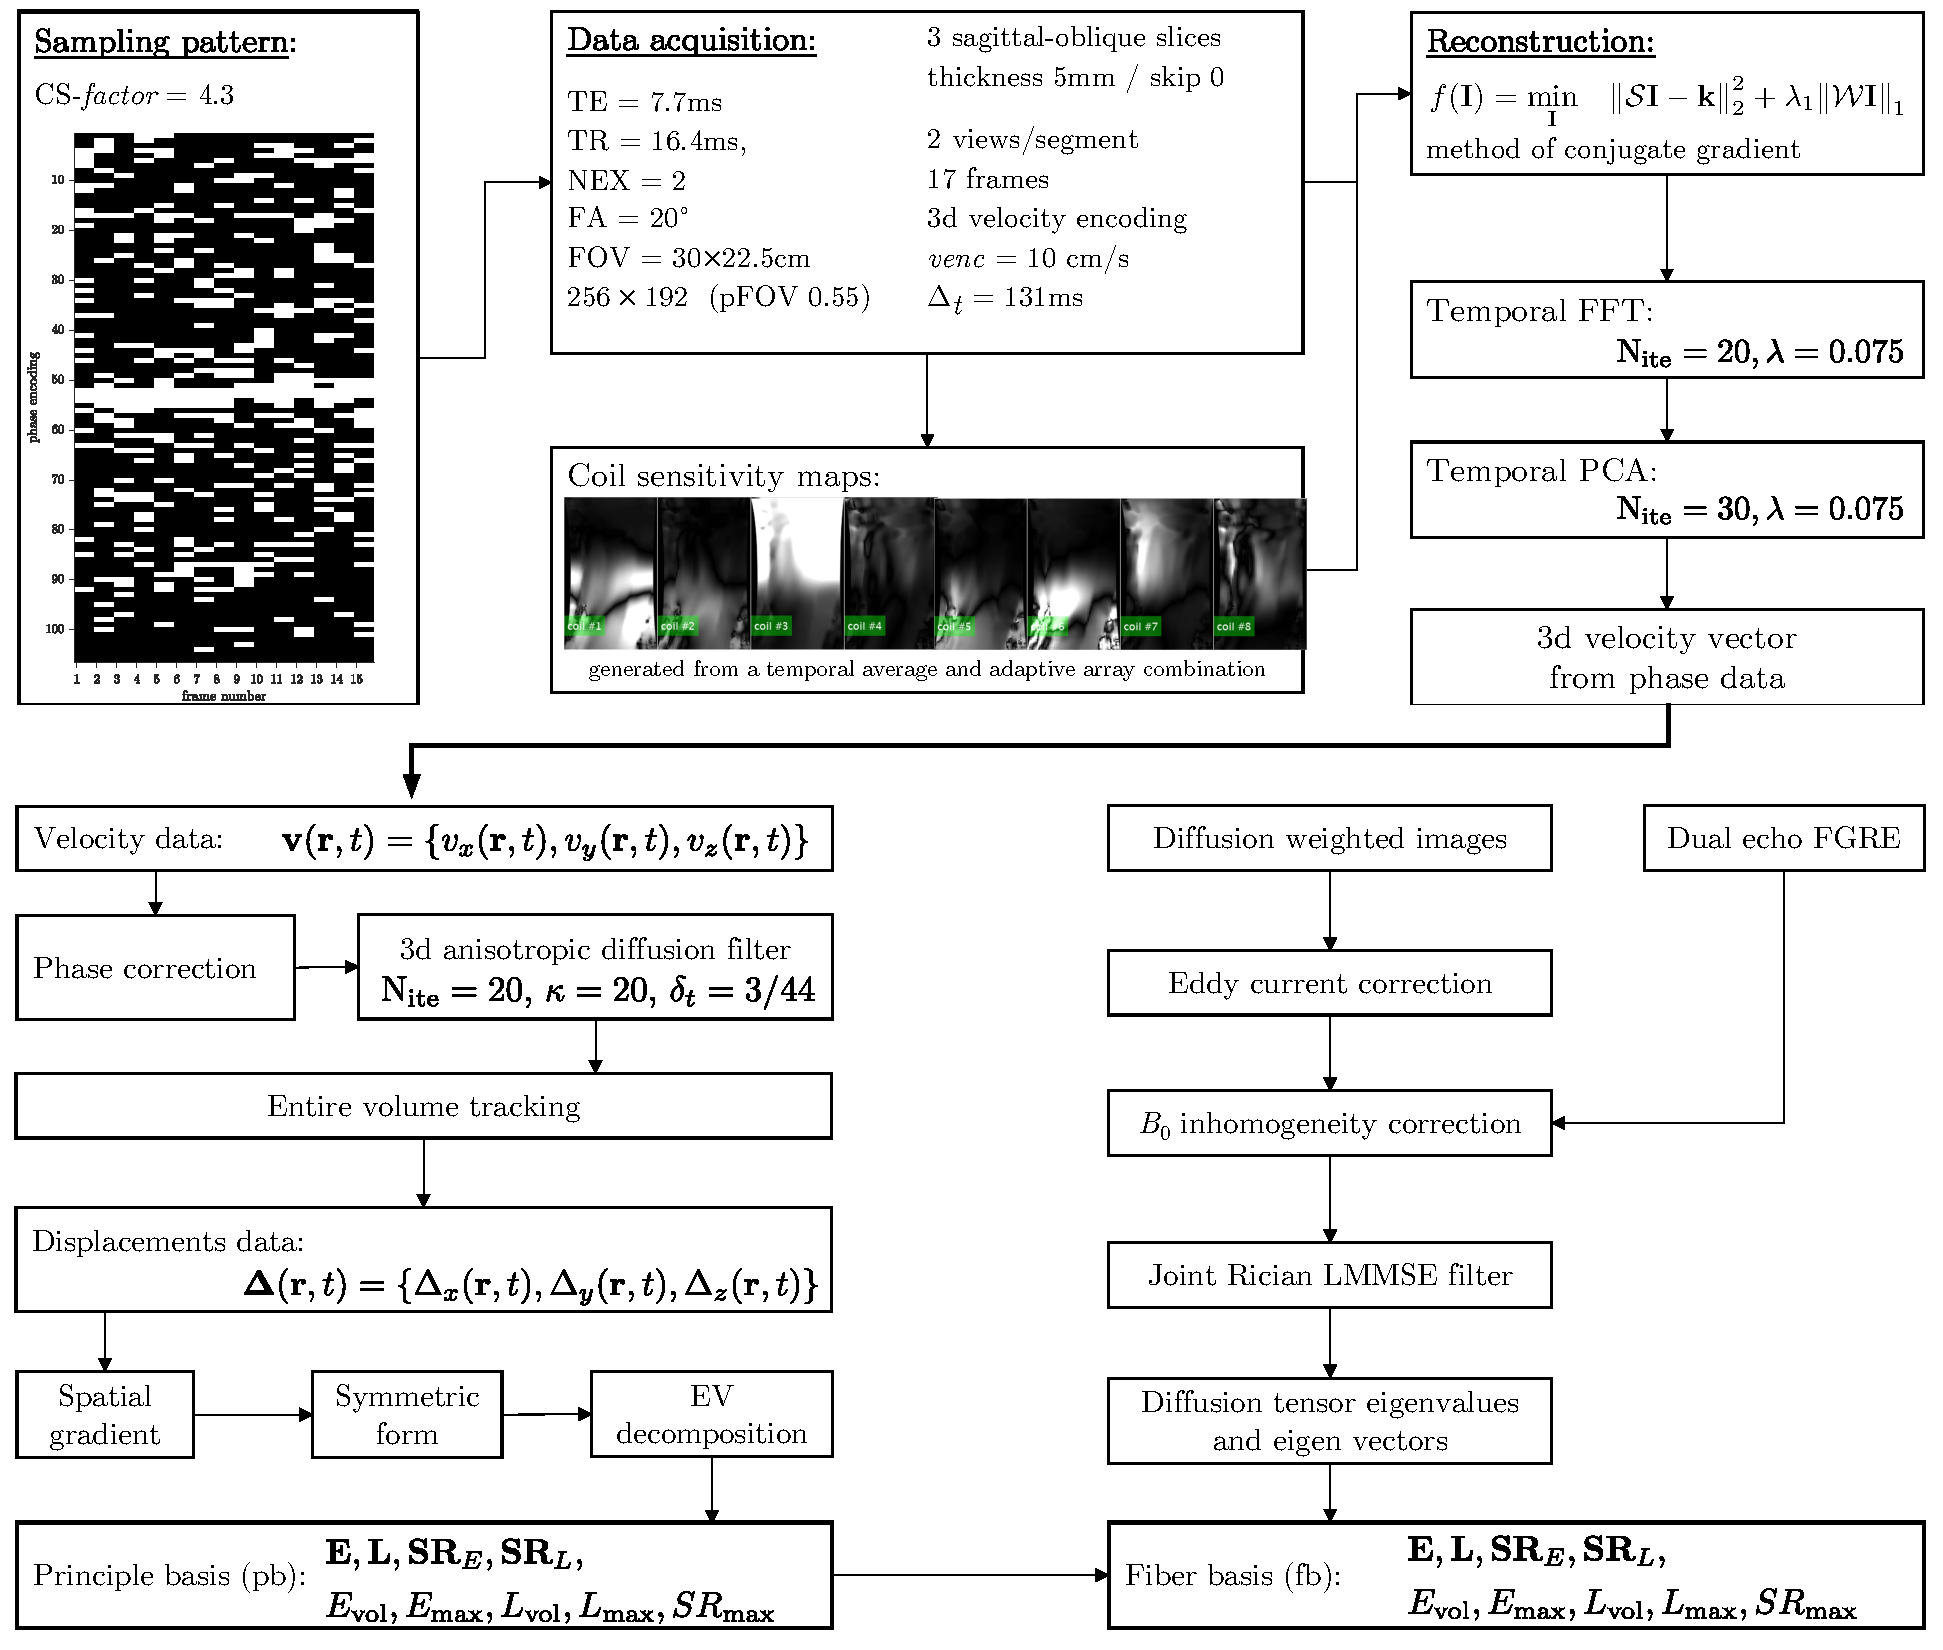
\includegraphics[scale=0.85]{Figures/CS2_1.pdf}
\caption[Pipeline of data acquisition and image processing for 3D strain/strain rate using undersampled VEPC sequence]{Pipeline of data acquisition and image processing for 3D strain/strain rate using undersampled VEPC sequence.}
\label{fig: CSYO1}
\end{sidewaysfigure}
%*********************************************************
Gated VEPC images were obtained during 3 sub-maximal isometric contraction levels.
VEPC acquisition was: echo time (TE): $\SI{7.7}{\milli\second}$, repetition time (TR): $\SI{17.8}{\milli\second}$, signal averages (NEX): 2, flip angle (FA): $\SI{20}{\degree}$, slice thickness: $\SI{5}{\milli\meter}$, field of view (FOV): $\SI{30}{\centi\meter} \times \SI{22.5}{\centi\meter}$ (partial phase FOV: 0.55), matrix $256 \times 192$ (lower resolution in the phase direction), 17 temporal frames (with view sharing factor = 2), $\SI{10}{\centi\meter/\second}$ three directional velocity encoding, 24 repetitions, cycle length $\SI{2.9}{\second}$.
Three contiguous slices were acquired at each \%MVIC for a total of nine dynamic acquisitions; each dynamic scan was 75 seconds resulting in $\times 8.6$ times accelerated acquisition (\mbox{CS\textit{-factor}} of 4.3, views per segment (VPS) = 2). 
The protocol also included a geometrically matched spin echo DTI EPI sequence.
The multi-coil CS scheme used a variable density random undersampling with maximum density at the center of \mbox{\textit{k-}space}. 
A two-step $k_y$\textit{-t} SENSE SPARSE CS joint reconstruction (of reference and velocity encoded images) was performed~\cite{RNCS10} using the coil sensitivities with a temporal FFT followed by a temporal PCA as the sparsifying transforms. 
The lower leg was resting against foot-pedal device~\cite{RNSS10} with strain sensor and anchored in an 8-channel RF coil; real-time visual feedback was provided to the subject. 
Data sets were obtained for sub-maximal forces (30, 40 and 60\% MVIC) for all subjects. 
3D strain and SR tensors were calculated for the central slice of the three acquired slices. 
Prior to the analysis, phase-contrast images were corrected for phase shading artifacts and denoised using a 3D anisotropic diffusion filter~\cite{RNCS17}.
Voxels in the entire volume were tracked to obtain displacements and locations in subsequent temporal frames. 
The 3D strain and SR images were generated from the spatial gradients of the velocity and displacement images; both Eulerian and Lagrangian strains and SR were evaluated. 
Two invariants were calculated from the rank 2 strain and SR tensors (volumetric and maximum shear strain rate $SR_{fc\_\,\mathrm{max}}$). 
The strain and strain tensors in principal axis were rotated to the DTI eigenvector frame of reference. 
The rotation matrix, R was generated from the DTI eigenvectors to reorient the strain and SR tensors from:
%.........................................................
\begin{equation}\label{eq: SRDTI}
SR_{\mathrm{fb}}=\mathrm{R_{DTI}}\cdot SR_{\mathrm{pb}} \cdot \mathrm{R_{DTI}}^\intercal
\end{equation}
%.........................................................
and components of the 3D strain rate tensor are:
%.........................................................
\begin{equation}
SR_{\mathrm{fb}} =\left[
\begin{array}{ccc}
SR_{ff} & SR_{fs} & SR_{ft} \\[4pt]
SR_{sf} & SR_{ss} & SR_{st} \\[4pt]
SR_{tf} & SR_{ts} & SR_{tt} \\
\end{array}\right]
\end{equation}
%.........................................................
Quantitative analysis was performed for a region of interest (ROI) placed in medial gastrocnemius and soleus muscles (7 $\times$ 7).
Indices were extracted at the frame corresponding to maximum $SR_\mathrm{fiber}$ during the contraction part of the cycle.
%~~~~~~~~~~~~~~~~~~~~~~~~~~~~~~~~~~~~~~~~~~~~~~~~~~~~~~~~~
\subsection{Results}
%~~~~~~~~~~~~~~~~~~~~~~~~~~~~~~~~~~~~~~~~~~~~~~~~~~~~~~~~~
Figure~\ref{fig: CSYO2} shows the $SR_\mathrm{fiber}$, $SR_\mathrm{in-plane}$ and $SR_{fc\_\,\mathrm{max}}$ maps respectively at 30 and 60 \%MVIC effort for one young and one senior subject; the maps correspond to the temporal frame at max $SR_\mathrm{fiber}$ in the contraction cycle.
%*********************************************************
\begin{sidewaysfigure}
\vspace{+0.2cm}
\centering
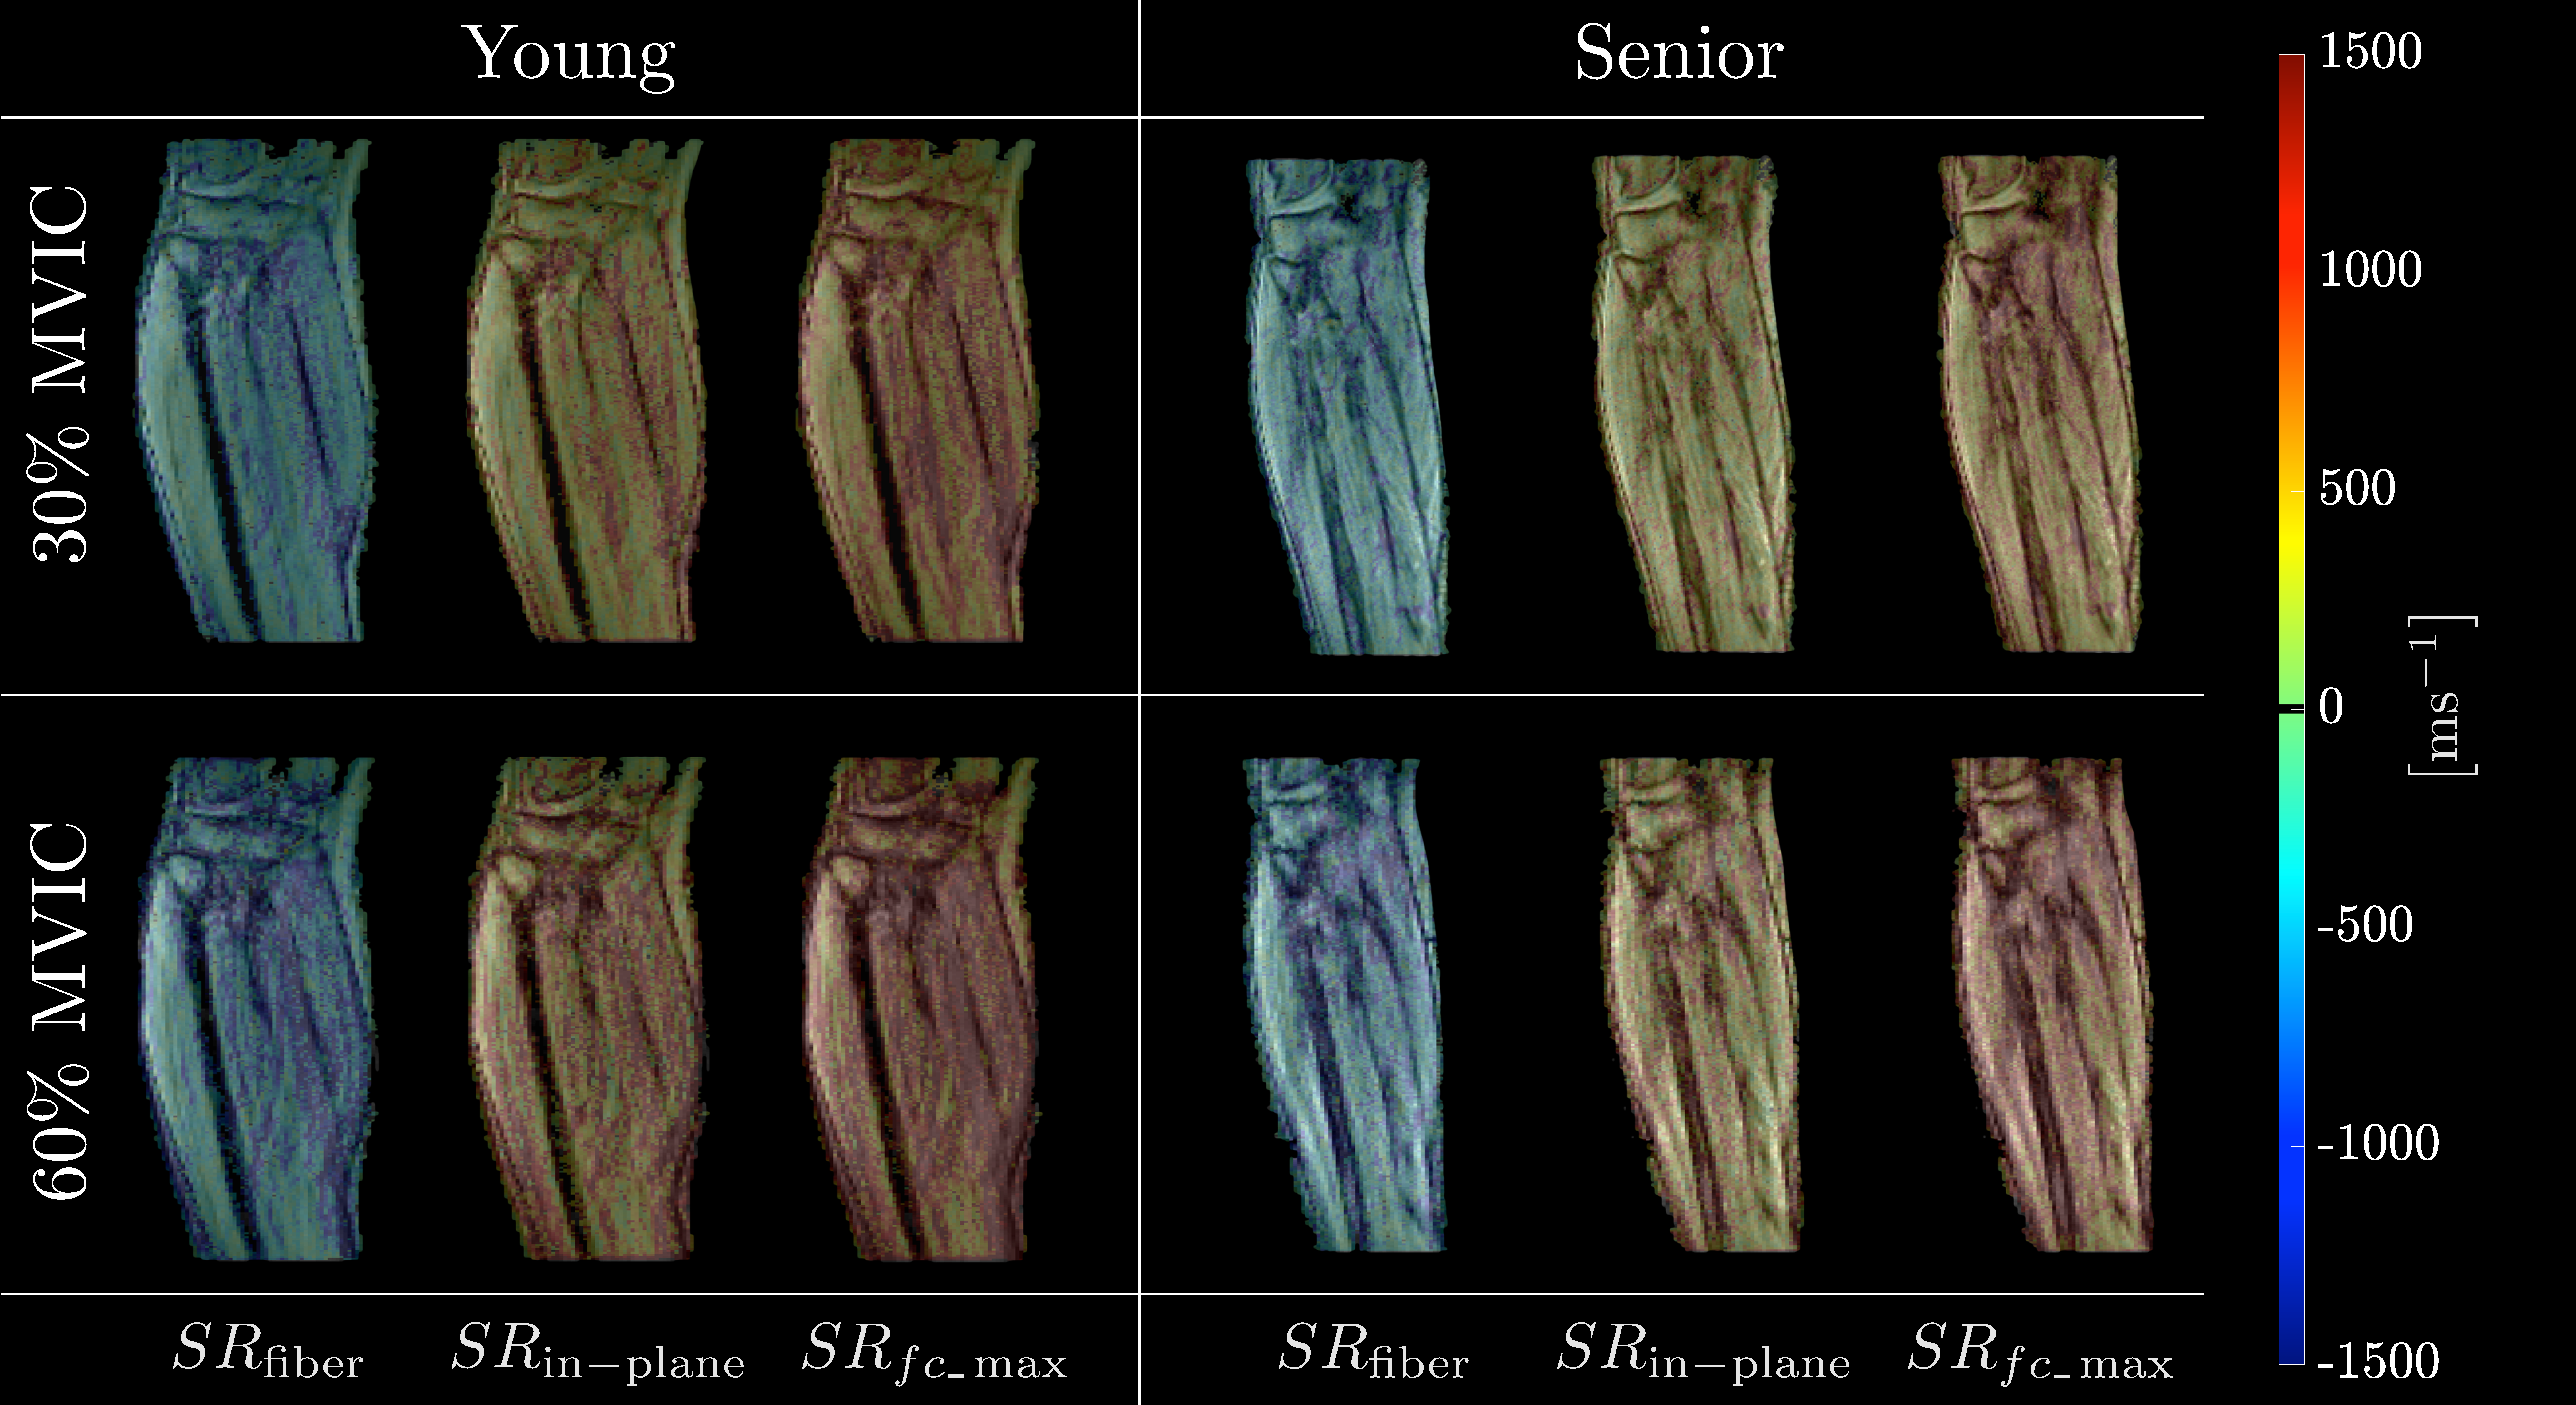
\includegraphics[width=8.5in]{Figures/CS2_2.pdf}
\captionsetup{width=8.5in}
\caption[Colormaps of the two strain rate eigenvalues $SR_\mathrm{fiber}$, $SR_\mathrm{in-plane}$ and invariant $SR_{fc\_\,\mathrm{max}}$ at 30\% and 60\% MVIC effort for one young and one senior subject]{Colormaps of the two strain rate eigenvalues $SR_\mathrm{fiber}$, $SR_\mathrm{in-plane}$ and invariant $SR_{fc\_\,\mathrm{max}}$ at 30\% and 60\% MVIC effort for one young subject and one senior; the maps correspond to the temporal frame at max $SR_\mathrm{fiber}$ in the contraction cycle.}
\label{fig: CSYO2}
\end{sidewaysfigure}
%*********************************************************
The quality of the SR eigenvalue colormaps underlines the efficiency of the CS reconstruction. 
Increase in eigenvalues with the increase in level of MVIC can be visually appreciated for subjects in both age groups. 
Figure~\ref{fig: CSYO4} shows colormaps of the diagonal components of SR in the fiber frame of reference for young and senior subject at the peak of the contraction.
%*********************************************************
\begin{sidewaysfigure}
\vspace{+0.2cm}
\centering
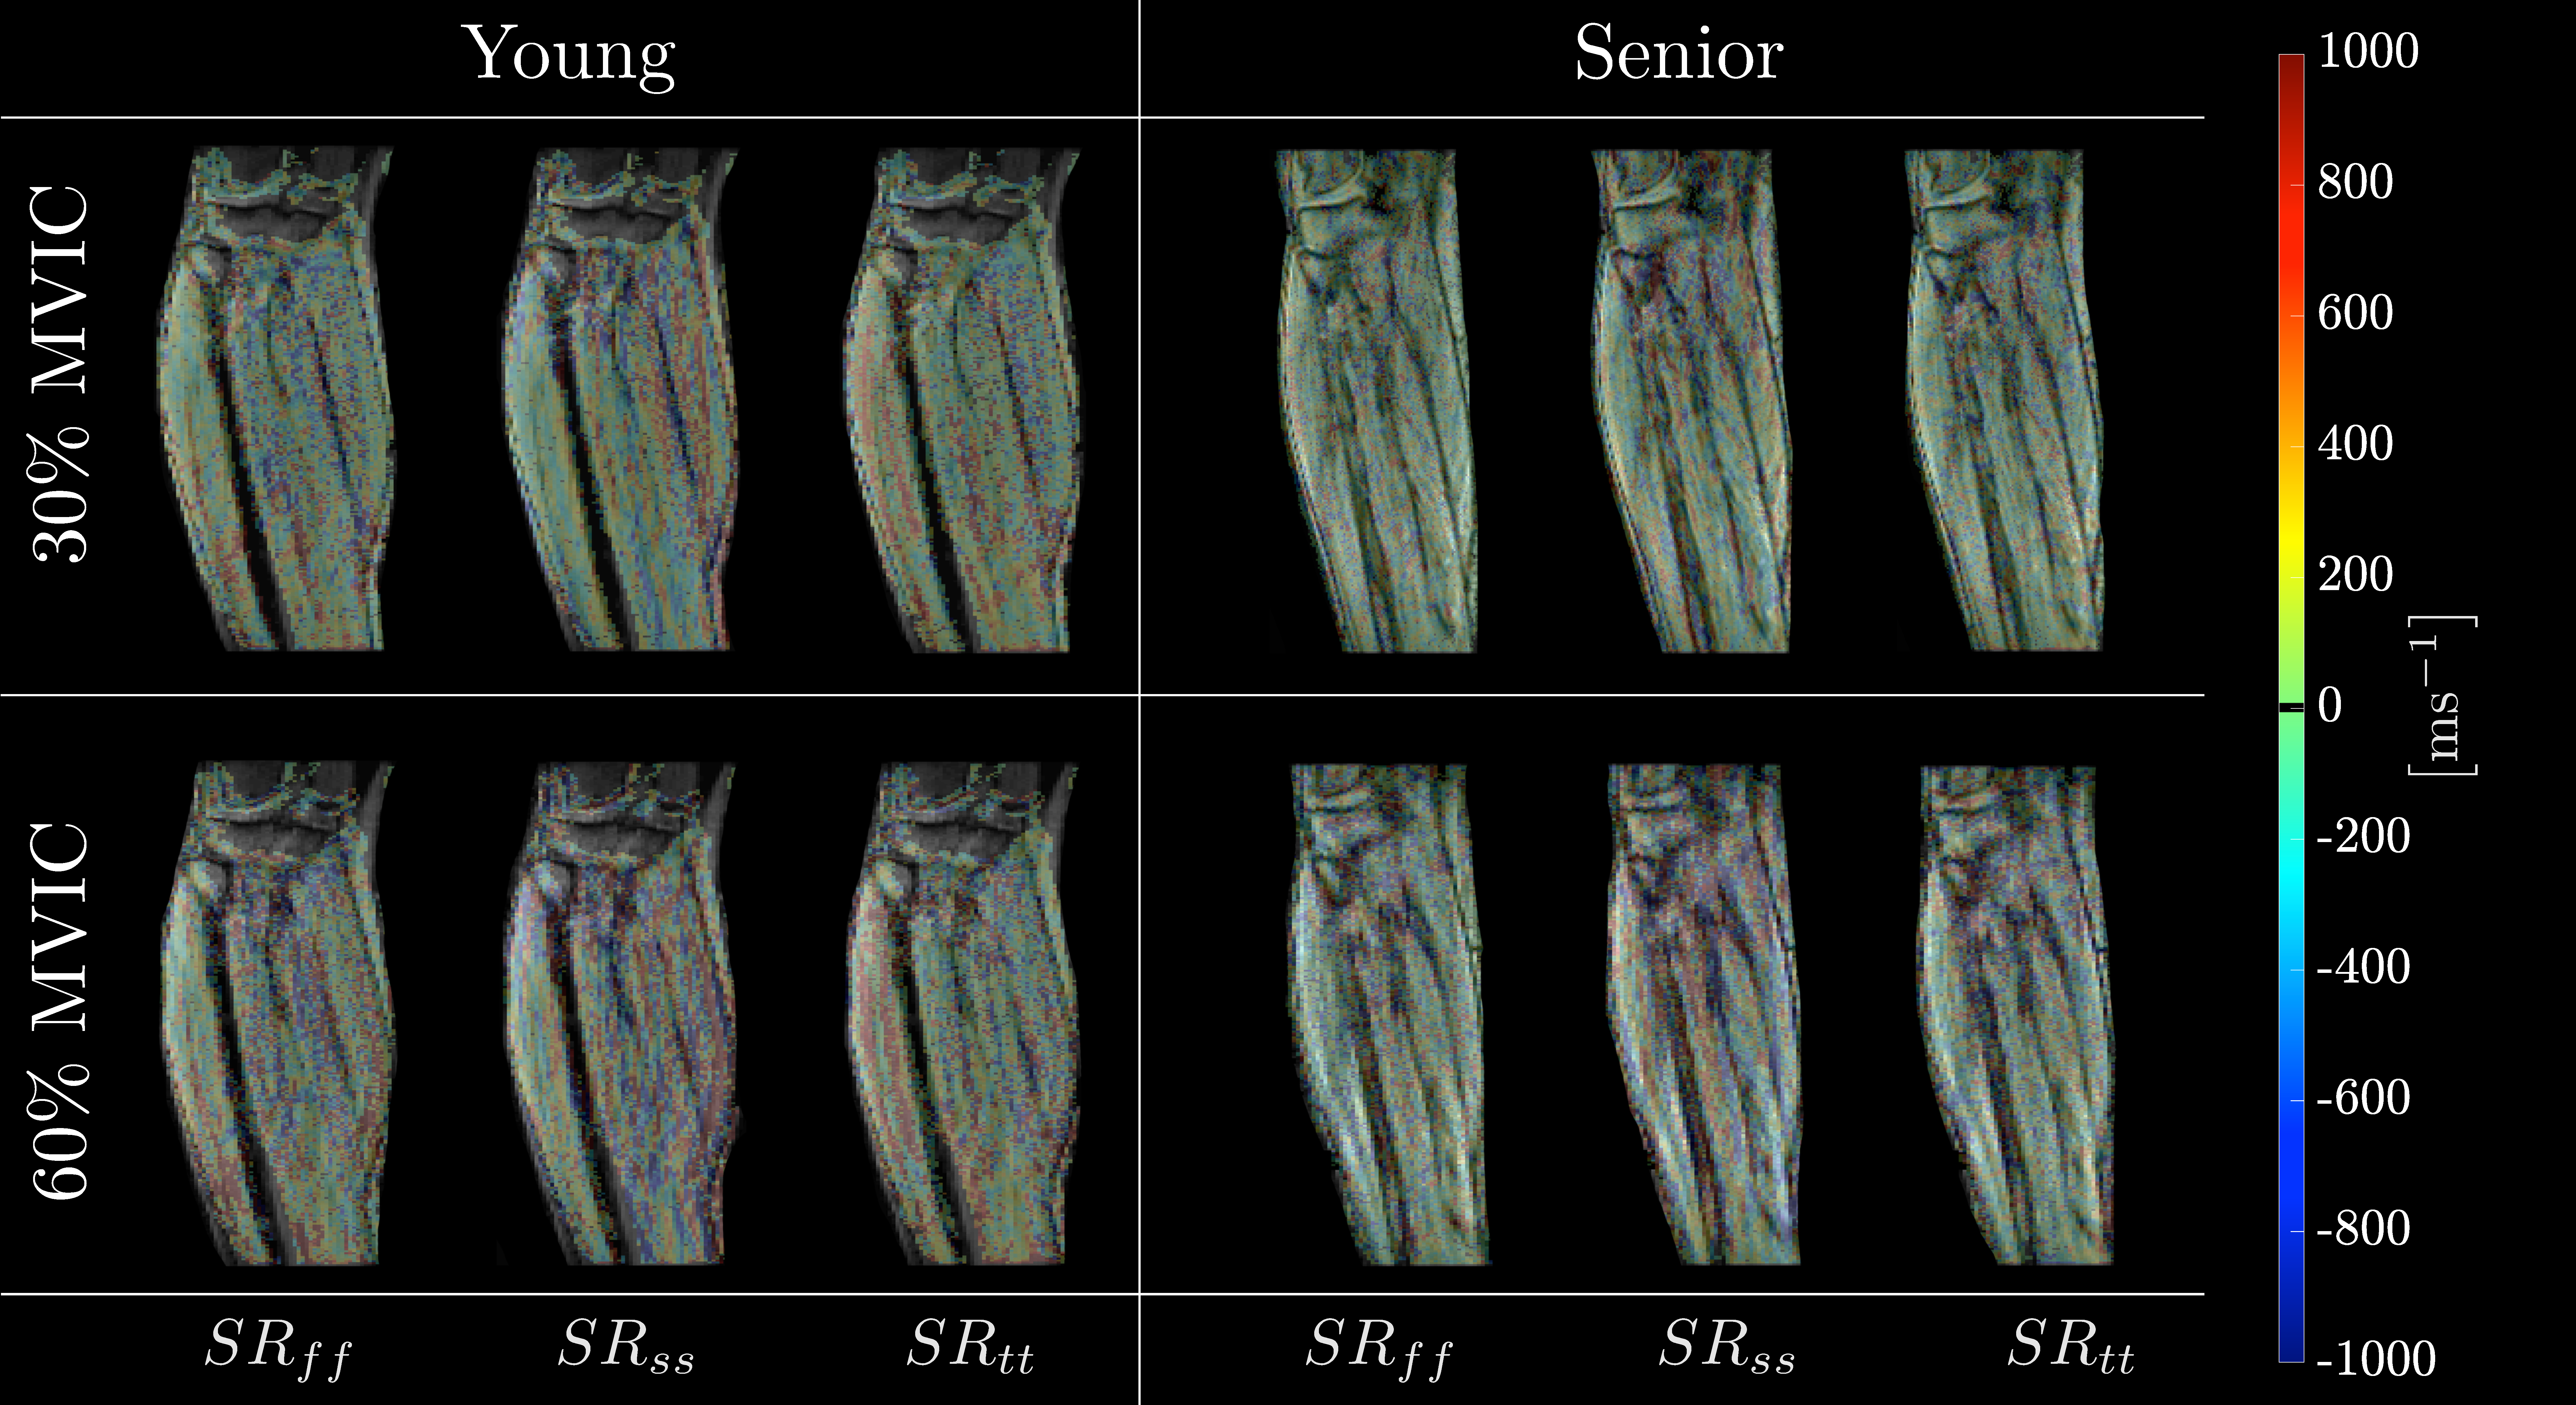
\includegraphics[width=8.5in]{Figures/CS2_4.pdf}
\captionsetup{width=8.5in}
\caption[Colormaps of the diagonal components of strain rate tensor in the fiber reference frame for one young and one senior subjects at two different levels of MVIC]{Colormaps of the diagonal components of strain rate tensor in the fiber reference frame for one young (left) and one senior (right) at two different levels of MVIC: 30\% (top row), 60\% (bottom row); the maps correspond to the temporal frame at max $SR_\mathrm{fiber}$ in the contraction cycle.}
\label{fig: CSYO4}
\end{sidewaysfigure}
%*********************************************************
Much smaller values of SR are seen in the fiber frame of reference and differences between young and senior are less than for components in principle frame. 
Table~\ref{tab: CSYO1} lists only the strain and strain rate indices (ROIs placed in the MG and Soleus) that were either significantly different between age groups and/or \%MVIC; no significant age*MVIC effect was seen.
%=========================================================
\begin{table}[!htb]
\vspace{+0.2cm}
\caption[Strain rate indices for two regions of interest in MG and SOL extracted at the the peak of the contraction]{Strain rate indices for two regions of interest in MG and SOL extracted at the temporal frame corresponding to $\max$ $SR_{\mathrm{fiber}}$ during the contraction phase.}
\label{tab: CSYO1}
\begin{center}
\begin{threeparttable}
\begin{tabular}{@{}lclrrrr@{}}
\toprule[1pt]\midrule[0.3pt]
\multicolumn{2}{l}{\multirow{2}{*}{}} & \multicolumn{1}{c}{\multirow{2}{*}{age}} & \multicolumn{2}{c}{MG}                                      &  \multicolumn{2}{c}{SOL}                                     \\ \cmidrule(lr){4-5} \cmidrule(lr){6-7} 
\multicolumn{2}{l}{}                  & \multicolumn{1}{c}{}                           & \multicolumn{1}{c}{30 \%MVIC} & \multicolumn{1}{c}{60\% MVIC} &  \multicolumn{1}{c}{30 \%MVIC} & \multicolumn{1}{c}{60\% MVIC} \\ \midrule[0.3pt]
\multirow{2}{*}{$\Delta_x$}\tnote{$1$, $2$, $4$}				& \multirow{2}{*}{$\left[\SI{}{\milli\meter}\right]$}   		 	& young     & $3.45 \pm 1.93$   & $6.78 \pm 3.53$  &  $2.54 \pm 1.03$  & $5.27 \pm 2.99$   \\
	  	  													&                  							     				& senior    & $2.54 \pm 2.23$   & $4.02 \pm 2.77$  &  $2.78 \pm 2.56$  & $3.84 \pm 2.90$   \\[4pt]
\multirow{2}{*}{$\Delta_y$}\tnote{$1$, $4$}					& \multirow{2}{*}{$\left[\SI{}{\milli\meter}\right]$}	   		& young     & $8.10 \pm 5.22$   & $10.14 \pm 4.74$ &  $5.89 \pm 1.98$  & $9.61 \pm 4.12$   \\
						    								&                   							     			  	& senior    & $5.05 \pm 3.40$   & $6.93 \pm 4.29$  &  $5.46 \pm 3.48$  & $7.65 \pm 4.67$   \\[4pt]
\multirow{2}{*}{$v_x$}\tnote{$1$, $2$, $4$}					& \multirow{2}{*}{$\left[\SI{}{\milli\meter/\second}\right]$} 	& young     & $9.22 \pm 4.91$   & $15.12 \pm 5.89$ &  $7.01 \pm 2.41$  & $13.05 \pm 5.56$  \\
															&                   							     				& senior    & $7.15 \pm 5.32$   & $9.89 \pm 6.16$  &  $7.51 \pm 7.25$  & $11.30 \pm 7.68$  \\[4pt]
\multirow{2}{*}{$v_y$}\tnote{$1$, $4$}						& \multirow{2}{*}{$\left[\SI{}{\milli\meter/\second}\right]$} 	& young     & $18.72 \pm 10.21$ & $23.37 \pm 7.49$ &  $14.50 \pm 3.82$ & $23.95 \pm 10.86$ \\
                  											&                   							     				& senior    & $12.49 \pm 8.05$  & $17.89 \pm 11.55$&  $12.86 \pm 9.34$ & $20.31 \pm 11.86$ \\[4pt]
\multirow{2}{*}{$E_{\mathrm{max}}$}\tnote{$1$}				&                   							     				& young     & $-0.92 \pm 0.49$   & $-1.60 \pm 0.57$  &  $-1.14 \pm 0.64$  & $-1.60 \pm 1.02$   \\
 				                    							&                   							     				& senior    & $-0.95 \pm 0.54$   & $-1.46 \pm 0.81$  &  $-1.01 \pm 0.65$  & $-1.21 \pm 0.93$   \\[4pt]
\multirow{2}{*}{$L_{\mathrm{max}}$}\tnote{$1$}				&                   							     				& young     & $-1.01 \pm 0.53$   & $-1.68 \pm 0.59$  &  $-1.16 \pm 0.59$  & $-1.65 \pm 1.02$   \\
                  											&                   							     				& senior    & $-1.02 \pm 0.56$   & $-1.57 \pm 0.85$  &  $-1.05 \pm 0.69$  & $-1.30 \pm 1.02$   \\[4pt]
\multirow{2}{*}{$SR_{fc\_\,\mathrm{max}}$}\tnote{$2$, $3$}	& \multirow{2}{*}{$\left[\SI{}{\per\milli\second}\right]$} 		& young     & $-197 \pm 83$   	& $-442 \pm 306$    &  $-283 \pm 227$    & $-400 \pm 263$     \\
                  											&                   							     				& senior    & $-244 \pm 165$  	& $-377 \pm 272$    &  $-209 \pm 157$    & $-261 \pm 155$     \\[4pt]
\multirow{2}{*}{$E_{\mathrm{fiber}}$}\tnote{$2$}	        		&                   							     				& young     & $-0.62 \pm 0.27$   & $-1.07 \pm 0.42$  &  $-0.60 \pm 0.31$  & $-0.92 \pm 0.56$   \\
                  											&                   							     				& senior    & $-0.59 \pm 0.33$   & $-0.94 \pm 0.51$  &  $-0.57 \pm 0.39$  & $-0.68 \pm 0.54$   \\[4pt]
\multirow{2}{*}{$L_{\mathrm{fiber}}$}\tnote{$2$}	        		&                   							     				& young     & $-0.66 \pm 0.27$   & $-1.12 \pm 0.43$  &  $-0.61 \pm 0.27$  & $-0.94 \pm 0.55$   \\
                  											&                   							     				& senior    & $-0.64 \pm 0.35$   & $-1.01 \pm 0.55$  &  $-0.59 \pm 0.41$  & $-0.74 \pm 0.61$   \\[4pt]
\multirow{2}{*}{$SR_{\mathrm{fiber}}$}\tnote{$2$, $3$}		& \multirow{2}{*}{$\left[\SI{}{\per\milli\second}\right]$} 		& young     & $-115 \pm 49$  	& $-263 \pm 170$   &  $-183 \pm 161$   & $-230 \pm 142$  \\
                  											&                   							     				& senior    & $-153 \pm 104$  	& $-234 \pm 176$   &  $-131 \pm 87$    & $-164 \pm 85$  \\[4pt]
\multirow{2}{*}{$SR_{\mathrm{in-plane}}$}\tnote{$2$, $3$}	& \multirow{2}{*}{$\left[\SI{}{\per\milli\second}\right]$} 		& young     & $120 \pm 52$   	& $258 \pm 194$    &  $154 \pm 110$    & $243 \pm 166$   \\
                  											&                   							     				& senior    & $137 \pm 91$   	& $211 \pm 140$    &  $118 \pm 103$    & $146 \pm 102$   \\ \midrule[0.3pt]\bottomrule[1pt]
\end{tabular}
\begin{tablenotes}[flushleft]\footnotesize
\item[$1$] Significant difference between age groups for MG.
\item[$2$] Significant difference between 30\% and 60\% MVIC for MG.
\item[$3$] Significant difference between age groups for SOL.
\item[$4$] Significant difference between 30\% and 60\% MVIC for SOL.
\end{tablenotes}
\end{threeparttable}
\end{center}
\vspace{-0.2cm}
\end{table}
%=========================================================
%~~~~~~~~~~~~~~~~~~~~~~~~~~~~~~~~~~~~~~~~~~~~~~~~~~~~~~~~~
\subsection{Discussion}
%~~~~~~~~~~~~~~~~~~~~~~~~~~~~~~~~~~~~~~~~~~~~~~~~~~~~~~~~~
Maximum shear strain rate $SR_{fc\_\,\mathrm{max}}$ (and shear strains), $SR_\mathrm{fiber}$ and $SR_\mathrm{in-plane}$ (and strains in-plane) were significantly lower with age and with \%MVIC (30 and 60\%MVIC). 
The source of the shear strain is hypothesized (based on computational models) to be the shear in the extracellular matrix; these models have also shown that shear strain is the mechanism of lateral transmission of force. 
The in-plane strain and $SR_\mathrm{in-plane}$ reflect the deformation in the fiber cross-section and will change with the mechanical properties of the extracellular matrix (stiffer ECM will restrict the in-plane deformation). 
%~~~~~~~~~~~~~~~~~~~~~~~~~~~~~~~~~~~~~~~~~~~~~~~~~~~~~~~~~
\subsection{Conclusions}
%~~~~~~~~~~~~~~~~~~~~~~~~~~~~~~~~~~~~~~~~~~~~~~~~~~~~~~~~~
Compressed sensing VE-PC enables dynamic acquisition of multi-slice/multiple levels of sub-maximal contraction in young and senior subjects. 
Significant differences with age seen in shear strains and in shear strain rates imply that the significant remodeling with age may occur in the extracellular matrix which could be a contributor to force loss. 
%~~~~~~~~~~~~~~~~~~~~~~~~~~~~~~~~~~~~~~~~~~~~~~~~~~~~~~~~~
\section{Acknowledgments}
%~~~~~~~~~~~~~~~~~~~~~~~~~~~~~~~~~~~~~~~~~~~~~~~~~~~~~~~~~
Section~\ref{sec: CS_paper} is a reprint of material, with minor edits as it appears in: V.~Malis, U.~Sinha, and S.~Sinha, ``Compressed sensing velocity encoded phase contrast imaging: Monitoring skeletal muscle kinematics,'' \emph{Magn. Reson. Med.}, Dec. 2019.
The author of the dissertation was the primary author of this paper.
%-new paragraph-%

%-new paragraph-%
Section~\ref{sec: CS_SRYO} is a reprint of material, with minor edits as it appears in: V.~Malis, U.~Sinha, and S.~Sinha, ``Principal Axis and Fiber Aligned 3D Strain / Strain Rate Mapping with Compressed Sensing Velocity Encoded Phase Contrast MRI to study Aging Muscle,'' \emph{Proceedings of the International Society of Magnetic Resonance in Medicine}, Sydney, 2020.
The author of the dissertation was the primary author of this abstract.
%#########################################################
\chapter{Diffusion Tensor Imaging}
\label{ch: Diffusion}
%#########################################################
Molecular diffusion in biological tissues is restricted due to interactions with many obstacles, such as fibers and neural tracts. 
Therefore diffusion patterns can be used to provide microscopic details about tissue architecture. This information is further used to detect abnormalities in skeletal muscles, heart and brain. 
MRI-based diffusion tensor imaging (DTI) is a relatively new modality, which allows the noninvasive \textit{in-vivo} determination of diffusion of water molecules arising from random motions due to the thermal energy of the tissue.
%-new paragraph-%

%-new paragraph-%
This chapter gives a brief introduction into diffusion theory and provides an overview of spin-echo and stimulated echo MR echo planar imaging pulse sequences that were used in the experiments discussed further in chapter~\ref{ch: DiffusionExp}.
%=========================================================
\section{Brownian Motion and Einstein Relation}
%=========================================================
In 1855 Adolf Fick explained diffusion through the flux of particles arising from the gradient of local concentration $c(\mathbf{r},t)$~\cite{Fick}:
%.........................................................
\begin{equation}\label{eq:Fick1}
\mathbf{J}=-D\nabla c(\mathbf{r},t)
\end{equation}
%.........................................................
For the total number of particles to be conserved divergence of the local flux should be related to the rate of change of $c(\mathbf{r},t)$ as $\nabla\mathbf{J}=-\frac{\partial c}{\partial t}$. This gives the diffusion equation:
%.........................................................
\begin{equation}\label{eq:Fick2}
\frac{\partial c}{\partial t}=D\nabla^2c
\end{equation}
%.........................................................
Equations~\ref{eq:Fick1} and \ref{eq:Fick2} are known as Fick's law. 
It was obtained for the case of admixture, when particles drift from higher to lower concentration regions, and this process is called \textit{mutual diffusion}. 
Albert Einstein in 1905 explained Brownian motion quantitatively~\cite{Einstein} and showed that Fick's laws are also valid for the case of \textit{self-diffusion}. 
Einstein described the motion of particles inside a finite volume $\delta V$ considering small displacements $\delta x$ due to the net force $K$, such that free energy is minimized: $\delta F=\delta E - T\delta S=0$. 
Utilizing the ideal gas model he related the work done by the particles with the change in entropy $\delta S = -k_B\frac{\partial V}{V}$. Thus the equilibrium condition is given:
%.........................................................
\begin{equation}\label{eq:EQ_Condition}
-Kn+k_BT\frac{\partial c}{\partial x}=0
\end{equation}
%.........................................................
where $k_B$ is Boltzmann's constant. The net flow of particles due to to net force $K$ is $J_{\mathrm{drift}}=\mu K $, where $\mu$ is mobility. Drift is counteracted by diffusive flow,  which according to Fick's law, is $J_{\mathrm{diff}}=-D\frac{\partial c}{\partial x}$. 
These flows are balanced and, together with equilibrium condition Equation~(\ref{eq:EQ_Condition}), result in a famous Einstein-Smoluchowski relation:
%.........................................................
\begin{equation}\label{eq:Einstein-Smoluchowski}
D=\mu k_BT
\end{equation}
%.........................................................
which was obtained independently by Albert Einstein~\cite{Einstein} in 1905, and Marian Smoluchowski~\cite{Smoluchowski} in 1906. 
For the small spherical particles of radius $r$, mobility is given by Stock's law $\mu=1/{(6\pi\eta r)}$, and Equation~(\ref{eq:EQ_Condition}) can be written in the following form:
%.........................................................
\begin{equation}\label{eq:Einstein-Stocks}
D=\frac{k_BT}{6\pi\eta r}
\end{equation}
%.........................................................
In addition to the expression for the diffusion coefficient, Einstein was able to describe  Brownian motion as a stochastic process~\cite{Einstein}. 
He considered conditional probability $P(\mathbf{r}|\mathbf{r'},t)$ for the particle at $\mathbf{r}$ at time $t_0=0$ to be at $\mathbf{r'}$ after time $t$. 
Local particle concentration~$c(\mathbf{r'}, t)$~is:
%.........................................................
\begin{equation}\label{eq:probability_concentration}
c(\mathbf{r'},t)=\int d\mathbf{r} \, c(\mathbf{r},0)P(\mathbf{r}|\mathbf{r'},t)
\end{equation}
%.........................................................
Since $c(\mathbf{r'},t)$ satisfies the diffusion equation Equation~(\ref{eq:Fick2}) for arbitrary choice of initial $c(\mathbf{r},0)$, the diffusion equation is also valid for probability $P(\mathbf{r'}|\mathbf{r}, t)$.
%.........................................................
\begin{equation}\label{eq:probability_diffusion}
\frac{\partial}{\partial t}P(\mathbf{r}|\mathbf{r'}t)=D\nabla^2P(\mathbf{r'}|\mathbf{r}, t)
\end{equation}
%.........................................................
With the initial condition $P(\mathbf{r'}|\mathbf{r}, 0)=\delta(\mathbf{r}-\mathbf{r'})$ the solution of the Equation~(\ref{eq:probability_diffusion}) is a Gaussian:
%.........................................................
\begin{equation}\label{eq:probability}
P(\mathbf{r}|\mathbf{r'},t)=\frac{1}{(4\pi Dt)^{3/2}} \mathrm{exp}\left( -\frac{(\mathbf{r'}-\mathbf{r})^2}{4Dt}\right)
\end{equation}
%.........................................................
From this equation, the mean square displacement is liner in time:
%.........................................................
\begin{equation}\label{eq:ms_dr}
\left<(\mathbf{r'}-\mathbf{r})^2\right>=6Dt
\end{equation}
%.........................................................
or in one dimension:
%.........................................................
\begin{equation}\label{eq:ms_dx}
\left<(x'-x)^2\right>=2Dt
\end{equation}
%.........................................................
The following definition of the diffusion coefficient flows from the Equation~(\ref{eq:ms_dx}):
%.........................................................
\begin{equation}\label{eq:D_v}
D=\lim_{t\rightarrow\infty}\frac{1}{2}\frac{\partial\left<\Delta x^2\right>}{\partial t}
\end{equation}
%.........................................................
Since $\Delta x = \int_0^t \mathrm{d}\tau \, v({\tau})$ the mean square displacement is:
%.........................................................
\begin{equation}\label{eq:D_v}
\left<\Delta x^2\right>=\int\limits_0^tdt_1\int\limits_0^tdt_2\left<v(t_1)v(t_2)\right>
\end{equation}
%.........................................................
By taking the derivative of this expression and using time translation invariance one can obtain Green-Kubo relation for diffusion coefficient $D$~\cite{Peliti}:
%.........................................................
\begin{equation}\label{eq:Green-Kubo}
D=\lim_{t \rightarrow \infty}\int\limits_0^\infty \mathrm{d} t \, \left<v(t) v(0)\right>
\end{equation}
%.........................................................
where $\left<v(t) v(0)\right>$ is the autocorrelation function of the molecular velocity $v$. In fact Equation~(\ref{eq:Green-Kubo}) represents a zero frequency component of the diffusion spectrum:
%.........................................................
\begin{equation}\label{eq:diffusion spectrum}
D(\omega)=\int\limits_0^\infty dt \, \left< v(t) v(0)\right> \mathrm{exp}(i\omega t) 
\end{equation}
%.........................................................
The correlation time is defined as:
%.........................................................
\begin{equation}\label{eq:correlation_time}
t_c=\int\limits_0^\infty dt \, \frac{\left<v(t) v(0)\right> }{\left< v^2\right>} 
\end{equation}
%.........................................................
and provides a timescale over which the fluctuating molecular velocity becomes decorrelated~\cite{DerekKJones}. 
This is an important result. 
In free solution, the correlation time is short. 
However, biological tissue molecules take much longer to thermalize because the length-scales of the spatial heterogeneities are typically much larger than the molecular scale. 
Thus in case of restricted diffusion, it's possible to access spectral features of the diffusion coefficient which provide detailed information even in case of complicated tissue architecture~\cite{Tuch:2002ts}.
%=========================================================
\section{Bloch-Torrey Equations and Diffusion Tensor}
%=========================================================
In 1950, just four years after the discovery of the NMR phenomenon by Bloch and Purcell~\cite{Bloch1946}, Ervin Hahn discovered that the spin-echoes he observed are sensitive to the effects of diffusion. 
He related the reduction of the signal to a dephasing caused by translational diffusion of spins subjected to local magnetic field gradients~\cite{Hahn}. 
In the presence of the diffusion term Bloch equations for the magnetization would change: 
%.........................................................
\begin{align}\label{eq:Bloch-Torrey}
\frac{dM_x}{dt}&=\gamma\left(\mathbf{M}\times B_0\right)_x-\frac{M_x}{\mathrm{T_2}}+D\Delta M_x\nonumber\\
\frac{dM_y}{dt}&=\gamma\left(\mathbf{M}\times B_0\right)_y-\frac{M_y}{\mathrm{T_2}}+D\Delta M_y\\
\frac{dM_z}{dt}&=\gamma\left(\mathbf{M}\times B_0\right)_z+\frac{M_0-M_z}{\mathrm{T_1}}+D\Delta(M_z-M_0)\nonumber
\end{align}
%.........................................................
This is so called Bloch-Torrey equations first introduced by Torrey in 1956~\cite{Torrey}.
Here $\mathbf{M}$ is the magnetization of a sample [\si{\ampere/\meter}], $B_0$ is a static magnetic field applied [\si{\tesla}], $\gamma$ is a gyromagnetic ratio [\si{\radian/\second \tesla}], $M_x$, $M_y$, $M_z$ are the $x$, $y$ and $z$ components of $\mathbf{M}, M_0$ is magnetization at thermal equilibrium and $\mathrm{T_1}, \mathrm{T_2}$ are the longitudinal and transversal relaxation times respectively. 
After \ang{90} radio frequency (RF) pulse is applied to the system, Bloch-Torrey equations give the following solution for the magnetization in the transverse plane:
%.........................................................
\begin{equation}\label{eq: dif_mag}
\bar{M}=M_0e^{-\frac{t}{T_2}}e^{-bD}
\end{equation}
%.........................................................
As opposed to the solution for the spin-echo Equation~(\ref{eq: dif_mag}) has an additional exponential factor $e^{-bD}$, \textit{b-}value identifies the measurement sensitivity to diffusion and determines the strength and duration of the diffusion gradients. The units of \textit{b-}value are [\si{\second/\milli\meter\squared}]:
%.........................................................
\begin{equation}\label{eq: b-value}
b=\gamma^2\int\limits_{0}^{\mathrm{TE}}dt\left(\int\limits_{0}^{t}dt'G(t')\right)^2
\end{equation}
%.........................................................
where $G$ is time-varying gradient of the magnetic field and $\mathrm{TE}$ is the echo-time.
Typical diffusion-weighted gradient consists of two lobes with equal area. In basic spin-echo sequences, two lobes ($G_{\mathrm{d1,2}}$) have the same polarity and are placed at either side of a refocusing RF-pulse as seen in Figure~\ref{fig: DTISeq}a. 
In gradient-echo sequences, however, the two lobes must have opposite polarity as shown in Figure~\ref{fig: DTISeq}b.
%*********************************************************
\begin{figure}[t]
\vspace{+0.2cm}
\centering
\includegraphics[width=\textwidth]{Figures/DiffusionPS.pdf}
\caption[Diffusion-weightning gradients in spin-echo and gradient echo pulse sequences]{Diffusion-weightning gradients in spin-echo and gradient echo pulse sequences.}\label{fig: DTISeq}
\end{figure}
%*********************************************************
An application of balanced bipolar gradients for the diffusion measurements was offered by Stejskal and Tanner~\cite{Stejskal}. 
Although the first gradient creates a spatially dependent phase to each spin the second gradient eliminates this effect for the stationary spins. 
Each of the protons experiencing a random diffusive displacement between the application of the two gradient pulses will acquire a phase offset proportional to the magnitude of the displacements. 
The result is phase dispersion proportional to the spread of positions. Thus, the diffusion coefficient $D$ along any direction can be measured by comparing MR signals $S(b)=M_0e^{-t/\mathrm{T_2}}e^{-bD}$ and $S(0)=M_0e^{-t/\mathrm{T_2}}$:
\begin{equation}\label{eq: Diffusion from bvalue}
D=-\frac{1}{b}\ln{\frac{S(b)}{S(0)}}
\end{equation}
%.........................................................
Until now diffusion coefficient $D$ was considered as a scalar in anisotropic medium. 
Biological tissues with regularly ordered microstructure such as skeletal muscle, spine, tongue, heart, white matter exhibit anisotropic water diffusion. 
An anisotropic media can be described in terms of tensor formalism. 
A diffusion tensor is a covariant tensor of $\rank$~2 that is described by a $3\times3$ symmetric matrix with 6 unique elements:
%.........................................................
\begin{equation}
\mathbf{D} =\left[
\begin{array}{ccc}
D_{xx} & D_{xy} & D_{xz} \\[4pt]
D_{yx} & D_{yy} & D_{yz} \\[4pt]
D_{zx} & D_{zy} & D_{zz} \\
\end{array}\right]
\end{equation}
%.........................................................
The components of the diffusion tensor can be calculated from the diffusion weighted image (DWI) set collected with the diffusion gradients applied in six or more directions. 
For the arbitrary number of gradient directions $n \geq 6$, the following system of liner equations can be written:
%.........................................................
\begin{align}
\begin{cases}
-\ln{\dfrac{S(b_1)}{S(b_0)}}&=\displaystyle\sum_{i,j=1}^3 b_{1ij}D_{ij}\\[2em]
-\ln{\dfrac{S(b_2)}{S(b_0)}}&=\displaystyle\sum_{i,j=1}^3 b_{2ij}D_{ij}\\
&\setbox0\hbox{=}\mathrel{\makebox[\wd0]{\vdots}} \\
-\ln{\dfrac{S(b_n)}{S(b_0)}}&=\displaystyle\sum_{i,j=1}^3 b_{nij}D_{ij}\\
\end{cases}
\end{align}
%.........................................................
where indexes $i$ and $j$ stand for $x,y$ and $z$ components.
Diffusion tensor yields several useful metrics. Mean Apparent Diffusion Coefficient (ADC) which gives the magnitude of the diffusion:
%.........................................................
\begin{equation}
\mathrm{ADC}=\frac{1}{3}\mathrm{Tr}\mathbf{D}
\end{equation}
%.........................................................
And  fractional anisotropy (FA) which is calculated after diffusion tensor eigenvalue decomposition is performed:
%.........................................................
\begin{equation}
\mathrm{FA}=\frac{\sqrt{3\displaystyle\sum_{i=1}^3 (\lambda_i-\mathrm{ADC})^2}}{\sqrt{2\displaystyle\sum_{i=1}^3 \lambda_i^2}}
\end{equation}
%.........................................................
where $\lambda_{1,2,3}$ are the eigenvalues of the diffusion tensor.
FA describes the degree of anisotropy and can take values between zero and one. 
Conventionally diffusion tensors are represented by ellipsoids.
%*********************************************************
\begin{figure}[h]
\vspace{+0.2cm}
\centering
\includegraphics[scale=0.8]{Figures/DiffusionFA.pdf}
\caption[Visual representation of the diffusion tensor in the isotropic and anisotropic cases]{Visual representation of the diffusion tensor in the isotropic and anisotropic cases.}\label{fig: AnisIso}
\end{figure}
%*********************************************************
\noindent If $\mathrm{FA} = 1$, then diffusion occurs only along one axis and is fully restricted along all others. $\mathrm{FA} = 0$ means an isotropic diffusion (Figure~\ref{fig: AnisIso}a). 
Biological tissues, such as muscle are anisotropic (Figure~\ref{fig: AnisIso}b) and diffusion mostly occurs along one of the eigenvectors, being restricted along the remaining two.
%=========================================================
\section{Echo Planar Imaging (EPI)}
\label{sec: EPI}
%=========================================================
A conventional MRI spin echo sequence acquires \textit{k}-space by sequential repetition of the basic spin echo pulse sequence ($\SI{90}{\degree}$ excitation RF-pulse followed by refocusing $\SI{180}{\degree}$). 
This sequence is too long compared to physiological (patient) motion. 
Addition of diffusion sensitization to routine spin echo sequence will essentially result in a completely wiped out image. 
In order to freeze motion, the established method for performing diffusion weighted imaging is to use a single shot technique, a spin echo echo-planar imaging (EPI) sequence, rather than a conventional spin echo.
%-new paragraph-%

%-new paragraph-%
Echo planar imaging (EPI) is the fastest MRI pulse sequence. 
With the modern hardware EPI allows producing of a 2D image as fast as tens of a millisecond. 
The main difference of EPI pulse sequence from the conventional pulse sequences (such as spin echo and gradient echo), is that the entire \textit{k}-space is acquired with one RF excitation (single-shot)~\cite{RNDT23}. 
This is accomplished by a series of bipolar readout gradients. 
To generate a train of gradient echoes (Figure~\ref{fig: EPI}a) with accompanying small phase-encoding gradients ('blips'), each gradient echo is distinctively spatially encoded so that multiple \textit{k}-space lines can be sampled under an RF spin echo (Figure~\ref{fig: EPI}b).
%*********************************************************
\begin{figure}[!h]
\vspace{+0.2cm}
\includegraphics[width=\textwidth]{Figures/EPI.pdf}
\caption[Spin-echo diffusion weighted EPI sequence and \textit{k}-space sampling path]{Spin-echo diffusion weighted EPI sequence and \textit{k}-space sampling path.}\label{fig: EPI} 
\end{figure}
%*********************************************************
EPI generates an image in a considerably shorter time than any other MRI sequence. 
Typical EPI pulse sequence is capable of producing $\sim 100$ gradient echoes as a result 2D image can be constructed from a single RF excitation~\cite{RNDT24}.
%-new paragraph-%

%-new paragraph-%
Compared to conventional MR imaging pulse sequences, EPI is more prone to a variety of artifacts. 
These artifacts arise from the fact the effective bandwidth in the phase-encoding direction is very small so that small differences in the frequency (other than from the phase encode gradient) at different spatial locations can result in severe mismapping. 
These frequency differences occur due to eddy currents from the large diffusion gradients, as well as from magnetic field inhomogeneities arising primarily from susceptibility differences in tissues and air. 
In my studies several correction techniques for eddy current, strong steady field inhomogeneity magnetic susceptibility were incorporated at the image pre-processing stage.
%-new paragraph-%

%-new paragraph-%
In spin-echo EPI sequence diffusion gradients are applied right before and immediately after $\SI{180}{\degree}$ refocusing pulse. 
As a result the range of the diffusion times is very constrained. 
Ability to measure diffusion tensor at diffusion times much longer compared to spin-echo EPI sequence provides an extra dimension in the data and a better estimate for micro-structural parameters.
%~~~~~~~~~~~~~~~~~~~~~~~~~~~~~~~~~~~~~~~~~~~~~~~~~~~~~~~~~
\subsection{Stimulated Echo Acquisition Mode (STEAM)}
%~~~~~~~~~~~~~~~~~~~~~~~~~~~~~~~~~~~~~~~~~~~~~~~~~~~~~~~~~
Compared to spin-echo which uses two RF-pulses Stimulated Echo~\cite{Hahn} uses three $\SI{90}{\degree}$ pulses with the same phase and observes total of five echos: three primary spin echos, one secondary and one simulated echo. 
All primary and a secondary echo experience $\mathrm{T_2^*}$ dephasing in between second and third RF-pulses while the magnetization forming stimulated echo is preserved along the longitudinal axis. 
The phase evolution of the magnetization in the pulse sequence with three RF-pulses is conveniently described using the diagram from~Figure~\ref{fig: STEAM_phase}.
%*********************************************************
\begin{figure}[!h]
\vspace{+0.2cm}
\centering
\includegraphics[width=\textwidth]{Figures/STEAM_Phase.pdf}
\caption[Spin-phase evolution diagram for the MR pulse sequence with three RF-pulses]{Spin-phase evolution diagram for the MR pulse sequence with three RF-pulses.}\label{fig: STEAM_phase} 
\end{figure}
%*********************************************************
 To keep only simulated echo pathway while eliminating signal from all the other four echoes as well as signal from free induction decays a set of four crusher gradients $\phi_{1-4}$ must be introduced. 
 For signal to be produced the accumulated phase due to the crusher must cancel out. 
 Phase dispersion created by a crusher gradient is directly proportional to its area thus by manipulating the size of the crusher gradients $\phi_{1-4}$ the stimulated echo pathway can be chosen while other echos can be destroyed.
%-new paragraph-%

%-new paragraph-%
 The stimulated echo signal pathway denoted SE in~Figure~\ref{fig: STEAM_phase}: first $\mathrm{RF_1}$ excites magnetization (1), next, phase is accumulated (2) due to gradient $\phi_1$, then $\mathrm{RF_2}$ reverses the phase (3) and locks magnetization longitudinally (4), following $\mathrm{RF_3}$ magnetization is restored in the transverse plane(5) and rephased by crusher gradient $\phi_4$ (6) to form an echo (7).
%-new paragraph-%

%-new paragraph-%
Conditions for stimulated echo are the following:
%.........................................................
\begin{equation}\label{eq: STEAM phase}
{\setstretch{1.0}
\begin{cases}
    \mathrm{E_1} &= -\phi_1 + \phi_2\\
    \mathrm{E_2} &= -\phi_1 + \phi_2 + \phi_3 - \phi_4\\
    \mathrm{E_3} &= -\phi_2 + \phi_3 + \phi_4\\
    \mathrm{E_4} &= -\phi_1 - \phi_2 - \phi_3 + \phi_4\\
    \mathrm{E_{1-4}} &\neq 0\\
    \mathrm{SE} &= -\phi_1 + \phi_4\\
    \phi_2 &\neq 0\\
    \phi_4 &\neq 0\\
\end{cases}
}
\end{equation}
%.........................................................
where first five equations are the conditions to destroy four echos, last two equations are conditions to remove signal originating from free induction decay and the equation for SE is the requirement to preserve stimulated echo. 
Diffusion weighting is added into the STEAM sequence by placing two identical diffusion gradients: first is placed in between $\mathrm{RF_1}$ and $\mathrm{RF_2}$ and second after $\mathrm{RF_3}$ pulse.
%~~~~~~~~~~~~~~~~~~~~~~~~~~~~~~~~~~~~~~~~~~~~~~~~~~~~~~~~~
\subsection{Correction to the \textit{b}-matrix}
\label{subsection: STEAM b value}
%~~~~~~~~~~~~~~~~~~~~~~~~~~~~~~~~~~~~~~~~~~~~~~~~~~~~~~~~~
In STEAM diffusion weighted sequence contribution to the \textit{b-}matrix (Equation~\ref{eq: bmatrix}) from cross-terms between different gradients becomes significant at long diffusion time $\Delta$ and must be calculated from the Equation~\ref{eq: b-value}. 
%.........................................................
\begin{equation}\label{eq: bmatrix}
b =\left[
\begin{array}{ccc}
b_{rr} & b_{rp} & b_{rs} \\
b_{pr} & b_{pp} & b_{ps} \\[1pt]
b_{sr} & b_{sp} & b_{ss} \\
\end{array}\right]
\end{equation}
%.........................................................
where indices $r, p, s$ are corresponding to three gradient axis: readout, phase encoding and slice selection respectively. 
%-new paragraph-%

%-new paragraph-%
Figure~\ref{fig: STEAM_GE} shows a plot of STEAM pulse sequence programmed in EPIC (GE Medical Systems, Milwaukee, WI, USA). 
Important timing parameters marked: diffusion time ($\Delta$) measured as time between diffusion gradients, duration of the diffusion gradients ($\delta$) and mixing time TM, measured as time between centers of the second and third RF-pulses.
%*********************************************************
\begin{figure}[h]
\vspace{+0.2cm}
\centering
\includegraphics[width =0.7\textwidth]{Figures/STEAM_GE.pdf}
\caption[Plot of STEAM pulse sequence programmed for GE scanner]{Plot of STEAM pulse sequence programmed for GE scanner.}\label{fig: STEAM_GE} 
\end{figure}
%*********************************************************
To satisfy conditions~\ref{eq: STEAM phase} the following configuration of crusher gradients was chosen:
%.........................................................
\begin{equation}\label{eq: bmatrix}
{\setstretch{1.0}
\begin{cases}
    \phi_1 = \phi_4\\
    \phi_1 \neq \phi_2\\
    \phi_2 \neq 0\\
    \phi_4 \neq 0\\
    \phi_2 \neq - \phi_3\\
    \phi_3 \neq \phi_2 - \phi_1\\
    \phi_3 \neq 2\phi_1 - \phi_2\\
    \phi_3 < \phi_2 < \phi_1
\end{cases}
}
\end{equation}
%.........................................................
Using full analytic form derived in~\cite{RNDT} independent components for \textit{b-}matrix due to diffusion, crusher and slice select gradient interactions are:
%.........................................................
\begin{equation}\label{eq: bmatrix}
{\setstretch{1.0}
\begin{array}{l}
    b_{rr} = \gamma^2\Bigl[G_{\mathrm{d}r}^2\tau_{11} + 2G_{\mathrm{d}r}G_{\mathrm{c}r}\tau_{12} + G_{\mathrm{c}r}^2\tau_{22}\Bigr]\\[10pt]
    
    b_{pp} = \gamma^2\Bigl[G_{\mathrm{d}p}^2\tau_{11} + 2G_{\mathrm{d}p}G_{\mathrm{c}p}\tau_{12} + G_{\mathrm{c}p}^2\tau_{22} \Bigr]\\[10pt]
    
    b_{ss} = \gamma^2\Bigl[G_{\mathrm{d}s}^2\tau_{11} +2G_{\mathrm{d}s}G_{\mathrm{c}s}\tau_{12} + G_{\mathrm{c}s}^3\tau_{22} + G_{\mathrm{sl}}^2\tau_{33} \Bigr]\\[10pt]
    
    b_{rp} = b_{pr} = \gamma^2\Bigl[G_{\mathrm{d}r}G_{\mathrm{d}p}\tau_{11} + \left(G_{\mathrm{c}p}G_{\mathrm{d}r} + G_{\mathrm{c}r}G_{\mathrm{d}p}\right)\tau_{12} + G_{\mathrm{c}r}G_{\mathrm{c}p}\tau_{22} \Bigr]\\[10pt]
    
    \begin{split}
	b_{rs} &= b_{sr} = \gamma^2\Bigl[G_{\mathrm{d}s}G_{\mathrm{d}r} \tau_{11} + \left( G_{\mathrm{d}s}G_{\mathrm{c}r} + G_{\mathrm{d}r}G_{\mathrm{c}s}\right)\tau_{12} + \\[2pt]
    	 	&\qquad\qquad\qquad\quad  + G_{\mathrm{c}r}G_{\mathrm{c}s}\tau_{22} + G_{\mathrm{sl}}G_{\mathrm{d}r}\tau_{13}+G_{\mathrm{sl}}G_{\mathrm{c}r}\tau_{23}\Bigr]
	\end{split}
    \\[4ex]
    \begin{split}
	b_{ps} &= b_{sp} = \gamma^2 \Bigl[G_{\mathrm{d}s}G_{\mathrm{d}p} \tau_{11} + \left( G_{\mathrm{d}s}G_{\mathrm{c}p} + G_{\mathrm{d}p}G_{\mathrm{c}s}\right)\tau_{12} + \\[2pt]
    	 	&\qquad\qquad\qquad\quad  + G_{\mathrm{c}p}G_{\mathrm{c}s}\tau_{22} + G_{\mathrm{sl}}G_{\mathrm{d}p}\tau_{13}+G_{\mathrm{sl}}G_{\mathrm{c}p}\tau_{23}\Bigr]\\[4pt]
	\end{split}
    \end{array}
}
\end{equation}
%.........................................................
with gradients amplitudes: $G_{\mathrm{d}*}$ and $G_{\mathrm{c}*}$ being diffusion and crusher pulses respectively where $*$ denotes gradient axis ($r,p$ or $s$), $G_{\mathrm{sl}}$ being an amplitude of a slice selection gradient pulse. 
Time constants $\tau_{ij}$ for the trapezoid gradient shape approximation are:
%.........................................................
\begin{equation}\label{eq: bmatrix timing}
{\setstretch{1.0}
\begin{array}{l}
	
	\tau_{11} = \delta_1^2\left( \Delta_1 - \dfrac{1}{3}\delta_1\right) + \dfrac{1}{30}\epsilon_{\mathrm{d}}^3-\dfrac{1}{6}\delta_1\epsilon_{{\mathrm{d}}}^2\\[12pt]
	\tau_{22} = \delta_2^2\left( \Delta_2 - \dfrac{1}{3}\delta_2\right) + \dfrac{1}{30}\epsilon_{\mathrm{c}}^3-\dfrac{1}{6}\delta_2\epsilon_{{\mathrm{c}}}^2\\[12pt]
	\tau_{12} = \delta_1\delta_2\Delta_2\\[12pt]
	\tau_{13} = \dfrac{1}{4}\delta_1\delta_{\mathrm{sl}}^2\\[12pt]
	\tau_{23} = \dfrac{1}{4}\delta_2\delta_{\mathrm{sl}}^2\\[12pt]
	\tau_{33} = \dfrac{1}{12}\delta_{\mathrm{sl}}^3\\[12pt]
\end{array}
}
\end{equation}
%.........................................................
where $\Delta_1$ is diffusion time, time constant $\Delta_2$ and pulse durations $\delta_{1,2}$ defined:
%.........................................................
\begin{equation}\label{eq: bmatrix timing delta}
{\setstretch{1.0}
\begin{array}{l}
	\Delta_{2} = \Delta_{1}-(\delta_{\mathrm{d}}+\delta_{\mathrm{c}})-2(\epsilon_{\mathrm{d}}+\epsilon_{\mathrm{c}})\\[12pt]
	\delta_{1} = \delta_{\mathrm{d}}+\epsilon_{\mathrm{d}}\\[12pt]
	\delta_{2} = \delta_{\mathrm{c}}+\epsilon_{\mathrm{c}}
\end{array}
}
\end{equation}
%.........................................................
$\delta_{\mathrm{d}}$ and $\delta_{\mathrm{c}}$ durations of the diffusion and crusher gradients, $\epsilon_{\mathrm{d}}$ and $\epsilon_{\mathrm{c}}$ rise time of the diffusion and crusher gradients, $\delta_{\mathrm{sl}}$ duration of the slice selection gradient.
	
	
%#########################################################
\chapter{Diffusion Modeling to Study Microarchitecture in Human Skeletal Muscles}
\label{ch: DiffusionExp}
%#########################################################
The resolution of the MR images is not sufficient to perform direct measurements of the muscle fiber geometry and other physical parameters such as membrane permeability at the level of individual fiber. 
While typical resolution of the MR images is $\approx \SI{e-3}{\m}$ histology studies showed that cross-sectional liner dimensions are in the range of $10^{-5} - \SI{e-4}{\m}$ \cite{TAYLOR200335}. 
In recent years a number of diffusion models were developed in the effort to relate macroscopic signal measured in MRI experiments to the microscopic parameters of muscle tissue. 
%-new paragraph-%

%-new paragraph-%
This chapter presents work on application of two diffusion models to interpret disuse atrophy and age related changes in human lower leg muscle.

%=========================================================
\section{Monitoring Changes in the Medial Gastrocnemius in Disuse Atrophy Induced by Unilateral Limb Suspension}
\label{sec: DTI ULLS}
%=========================================================
The feasibility of diffusion tensor imaging (DTI) of skeletal muscle including muscle fiber tracking for extraction of fiber lengths and pennation angles has been established, and the technique has been applied to monitor muscle injury, aging, gender related differences, and compartmental syndrome~\cite{RND1, RND2, RND3, RND4, RND5, RND6}. 
Additionally, some studies have explored changes in muscle DTI with atrophy; e.g., arising from age-related atrophy in human skeletal muscle~\cite{RND7}, from denervation and from Achilles tenotomy-induced atrophy in rodent models~\cite{RND8, RND9}.
Further, DTI combined with diffusion models is increasingly being used to explore tissue microstructural parameters such as fiber diameter, permeability or intracellular volume fraction~\cite{RND10}.
While most modeling studies have focused on the brain, a few recent studies have extended modeling efforts to the diffusion in skeletal muscle~\cite{RND11, RND12, RND13}. 
Recent studies have combined combine magnetic resonance imaging deformation analyses and diffusion tensor imaging tractography in the medial gastrocnemius~\cite{RNSS4,RNCS4}. 
Karakuzu~et~al. showed that submaximal plantar flexion activity at 15\% Maximum voluntary contraction (MVIC) causes heterogeneous length changes along the fascicles of human medial gastrocnemius (MG) muscle~\cite{RNCS4}.
The heterogeneity of fascicle strains was explained on the basis of epimuscular myofascial force transmission. 
%-new paragraph-%

%-new paragraph-%
It is well established that disuse (e.g., by chronic unloading) leads to skeletal muscle atrophy that is accompanied by a significant loss of muscle force~\cite{RNS1}.
The Unilateral Limb Suspension (ULLS) is a validated model to study the effects of chronic unloading~\cite{RNS8}.
Unilateral limb suspension results in both loss of muscle mass (muscle fiber atrophy) as well as a decrease in muscle force~\cite{RNS8}.
Prior studies of induced immobilization indicate that muscle remodeling with inactivity is a fast process that occurs after about a week of unloading~\cite{RNS8, RNS5}.
These studies documented the decrease in both fiber length and pennation angle, a decrease in Focal Adhesion Kinase content ($-20\%$) and activity ($-30\%$), associated with a $50\%$ fall in muscle protein synthesis and a $5\%$ decrease in quadriceps muscle anatomical cross-sectional area (ACSA)~\cite{RNS8, RNS5}.
DTI with its ability to probe at the microstructural level is ideally suited to investigate potential muscle remodeling that occurs with chronic unloading.
However, no studies to date have investigated unloading induced changes in skeletal muscle using DTI in human subjects.
%~~~~~~~~~~~~~~~~~~~~~~~~~~~~~~~~~~~~~~~~~~~~~~~~~~~~~~~~~
\subsection{Methods}
%~~~~~~~~~~~~~~~~~~~~~~~~~~~~~~~~~~~~~~~~~~~~~~~~~~~~~~~~~
%---------------------------------------------------------
\subsubsection{\textit{In-vivo} experiments}
%---------------------------------------------------------
The study was carried out under the approval of the Medical Research Ethics Board of UC~San~Diego and conformed to all standards for the use of human subjects in research as outlined in the Declaration of Helsinki on the use of human subjects in research.
IRB approval was obtained from the Medical Research Ethics Board of UC~San~Diego and all subjects were recruited after obtaining written informed consent. A total of 7 normal healthy young subjects (2 females, $29.1 \pm 5.7$ years, body mass $75.4 \pm \SI{22.7}{\kilogram}$, height $168.1 \pm \SI{7.4}{\centi\meter}$) were recruited for this study.
The criterion for inclusion was that subjects should be moderately physically active. Subjects participating in competitive sports as well as those with any surgical procedures performed on the lower leg were excluded.
%---------------------------------------------------------
\subsubsection{Study design} 
%---------------------------------------------------------
The effect of chronic unloading on the force production capability and diffusion tensor indices of the MG muscle were assessed by comparing the baseline (pre) to immediately after four weeks of limb suspension (post).
During the four week suspension period, subject compliance to the protocol was monitored at two weeks to check for muscle atrophy (MRI morphological scan) and loss of force production.
In addition, compliance was also monitored by a wireless activity tracker that was integrated into the crutches; the subject was not informed of the tracker to ensure that it was not removed or tampered with to simulate crutch usage.
After the four week suspension, subjects were required to attend structured physical rehabilitation sessions.
MRI morphological scans were performed at the end of the rehabilitation period (four weeks) to confirm that the muscle had recovered to baseline status.
%---------------------------------------------------------
\subsubsection{Unilateral Limb Suspension (ULLS)}
%---------------------------------------------------------
The ULLS model is an established model of inducing controlled atrophy~\cite{RNS19} and was used in the current study to induce muscle atrophy on the non-dominant leg with four weeks of chronic unloading.
The dominant leg was self-identified by subjects as the one they preferentially used to regain balance from a jostle.
The non-dominant leg was the left leg for all subjects in this study.
The ULLS protocol allowed the subjects a reasonable amount of freedom to carry out their daily activities including driving since the dominant leg (right in this study) was not unloaded.
A crutch was used to prevent the foot (of the left leg) from touching the ground.
The right foot was raised with a $\SI{5}{\centi\meter}$ sole on the shoe to further minimize accidental loading of the foot.
%---------------------------------------------------------
\subsubsection{MR imaging} 
%---------------------------------------------------------
Subjects were positioned supine in a $\SI{3}{\tesla}$ whole-body scanner (GE Medical Systems, WI, USA) and only the limb selected for suspension was scanned (pre- and post-suspension).
A custom-built receive-only phased array coil with a large FOV was used to image approximately $\SI{30}{\centi\meter}$ of the lower leg without moving the subject or coil; the intent was to cover the medial gastrocnemius muscle from its origin to insertion in two acquisitions without having to reposition the subject in the coil.
The coil moved relative to the magnet between acquisitions, the subject did not move with respect to the coil.
One anatomical slice was common between the two sets of acquisitions and the two sets were reoriented by a transformation obtained from the rigid alignment of the slice common to both sets.
The subject's leg was fully extended while the foot was maintained in a fixed position at $\approx \SI{15}{\degree}$ in plantarflexion; the foot rested on an adjustable wedge to maintain the angle constant for the scan duration. This foot position was used to ensure that there was no passive tension in the lower leg muscles.
%-new paragraph-%

%-new paragraph-%
The MRI pulse sequence used in the image acquisition was a fat suppressed single shot EPI spin-echo sequence with monopolar diffusion gradients (diffusion gradient duration, $\delta = \SI{12}{\milli\second}$, and diffusion time $\Delta = \SI{20}{\milli\second}$). 
Spectral-spatial water selective excitation was used to suppress fat.
The total number of slices (acquired in two multi-slice 2D sets) required to cover the calf muscles ranged from 32 to 40 slices.
$B_0$ shimming in the selected region of interest was performed with vendor supplied automated second order shims.
Thirty-two non-collinear gradient directions with a \mbox{\textit{b-}value} of $\SI{400}{\second \per \milli\meter^2}$ were used to map the direction dependent diffusion.
Imaging parameters: echo time (TE) $\SI{52.7}{\milli\second}$, repetition time (TR) $\SI{7000}{\milli\second}$ ms with 4 signal averages, field of view (FOV) $240 \times 240 \; \SI{}{\milli\meter^2}$, slice thickness $\SI{5}{\milli\meter}$, no gap and acquisition matrix $80 \times 80$; no parallel imaging was employed. The $80 \times 80$ matrix was reconstructed to $128 \times 128$ matrix by partial fourier with homodyne reconstruction.
The homodyne algorithm pre-weights the \mbox{\textit{k-}space} data so that when the real part of the image is extracted, it corresponds to uniform weighting in \mbox{\textit{k-}space}~\cite{RND20}.
The $128 \times 128$ matrix is then extrapolated to a $256 \times 256$ matrix yielding a voxel resolution of $\SI{0.94}{\milli\meter} \times \SI{0.94}{\milli\meter} \times \SI{5.00}{\milli\meter}$.
In addition to the diffusion weighted images, a morphological volume was acquired with a fat saturated fast gradient echo (FGRE) sequence for two echo times with the following parameters: $\mathrm{TE_1}/\mathrm{TE_2}$/TR: $\SI{3.2}{\milli\second}/\SI{5.6}{\milli\second}/\SI{350}{\milli\second}$ and a flip angle (FA) of $\SI{20}{\degree}$; all geometric parameters were the same as in the DTI scans.
The acquired morphological volume was used to generate phase maps to correct $B_0$ distortions in the echo planar images.
The total scan time including the morphological images for each session was 17 minutes. 
%---------------------------------------------------------
\subsubsection{Force measurements}
%---------------------------------------------------------
Isometric MVIC of the plantarflexor muscles was determined for each subject prior to MR imaging. For this purpose, the ankle was fixed in a neutral position ($\SI{90}{\degree}$ angle between the axis of the foot and the shank).
To estimate the maximum force acting along the Triceps Surae tendon, the force recorded by the force transducer was divided by the Achilles tendon moment arm corresponding to $\SI{90}{\degree}$ angle between the axis of the foot and the shank detailed earlier~\cite{RNS20}.
In brief, a sagittal MR image of the lower leg and foot was used to identify the joint (ankle) center of rotation as well as Achilles tendon line of action (the latter marked as a straight line along the center of the tendon). 
The perpendicular distance of the joint center to the line of action was measured as the Achilles tendon moment arm~\cite{RNS20}.
The measured muscle force is that generated by the gastrocnemius (lateral and medial) and the soleus muscles.
%---------------------------------------------------------
\subsubsection{Muscle volume measurements}
%---------------------------------------------------------
The manual contouring was performed using parametric Bezier curves every fifth slice using OsiriX~\cite{RND22}.
Automated interpolation was performed for the intervening slices; all automated contours were examined and edited if needed.
%---------------------------------------------------------
\subsubsection{Image preprocessing and DTI indices computation}
%---------------------------------------------------------
Figure~\ref{fig: DTI-flowchart} is the flowchart of the sequence of image processing steps.
All diffusion weighted image volumes were registered to the baseline ($b=0$) image to correct for eddy currents and motion related artifacts using the \textit{eddy} algorithm from FSL~\cite{RND23}. 
The phase images of the dual echo (FGRE) volumes were used to correct for $B_0$ field inhomogeneities using the \textit{fugue} algorithm from FSL~\cite{RND23}.
Diffusion weighted images were then denoised using a Joint Rician Linear Minimum Mean Square Error (LMMSE) estimator~\cite{RND24}. 
The noise in magnitude MR images is best modeled by a Rician distribution and the LMMSE estimator has been shown to out-perform other Rician denoising techniques~\cite{RND25}.
The tensor was calculated from the distortion corrected and denoised data using a Gaussian model of diffusion.
The tensor was then diagonalized to yield the eigenvalues followed by the calculation of the fractional anisotropy (FA), apparent diffusion coefficient (ADC) and coefficient of planarity (CP) maps. 
The contour of the MG traced in the FGRE volume slices was transferred to the DTI indices map.
Average values of the DTI indices were obtained from a $5 \times 5$ region of interest (ROI) automatically placed at the centroid of the MG mask at each anatomical slice (in most subjects, 40 axial slices were required to cover the MG); this placement ensured that the ROI was not at the edges which would bias estimates due to partial volume effects. 
A manual check was also made to ensure that the ROI was not in the region of a blood vessel, fascia or contained artifacts; such ROIs were moved manually to avoid artifacts. 
Though the ROI was small at 25 pixels/slice, the total number of pixels across all slices was $\approx 900 (25 \times 36)$ ensuring the robustness of the DTI indices. 
%*********************************************************
\begin{figure}[!htb]
\vspace{+0.2cm}
\centering
\includegraphics[width=0.9\textwidth]{Figures/DTI_flowchart.pdf}
\caption[The image processing flowchart showing the sequence of steps leading to the extraction of the diffusion tensor indices]{The image processing flowchart showing the sequence of steps leading to the extraction of the diffusion tensor indices.}
\label{fig: DTI-flowchart}
\end{figure}
%*********************************************************
%---------------------------------------------------------
\subsubsection{Simulation}
%---------------------------------------------------------
The model used here closely follows that proposed originally by Karampinos~et~al.~\cite{RND12}. 
Simulations were carried out by varying the fit parameters ($\alpha$, $d$, $\tau_{\mathrm{in}}$, $\nu_{\mathrm{in}}$, $\nu_{\mathrm{col}}$) to compute DTI eigenvalues. 
The five parameter-space was searched to find the optimal combination of the five parameters that minimized the normalized root mean square difference (NRMSE) between the eigenvalues computed from the simulation and those determined from experiments (Equation~\ref{eq: KargerRMSE}).
%.........................................................
\begin{equation}\label{eq: KargerRMSE}
\mathrm{NRMSE} = \sqrt{\dfrac{\sum\limits_{i=1}^3 \left( \lambda_{i,\mathrm{expr}}-\lambda_{i, \mathrm{sim}} \right)^2}{\sum\limits_{i=1}^3 \lambda_{i,\mathrm{expr}}^2}}
\end{equation}
%.........................................................
where $\lambda_{i,\mathrm{expr}}$ is the experimentally determined eigenvalues while $\lambda_{i,\mathrm{sim}}$ is the eigenvalue from the model simulation. 
Since there are five variables that are fit to the model, the search space was limited to physiologically relevant ranges in order to prevent the search from minimizing at non-physiological values, these ranges were taken from~\cite{RND12}. 
The simulations were carried out with the values for intra-cellular diffusion coefficient ($D_{\mathrm{in}}$), extracellular matrix diffusion coefficient ($D_{\mathrm{ex}}$), intra-cellular $\mathrm{T_2}$ ($\mathrm{T}_{\mathrm{2,in}}$), and extra-cellular $\mathrm{T_2}$ ($\mathrm{T}_{\mathrm{2,ex}}$) taken from the literature~\cite{RND12, RND26}.
It should be noted here that Karampinos~et~al. fitted $D_{\mathrm{in}}$ and $D_{\mathrm{ex}}$ to the diffusion model, but these variables were kept fixed in the current paper at the values obtained for young normal subjects in the former paper~\cite{RND12}. 
This was done to limit the number of model variables in order to increase the robustness of the fit.
Further, as $D_{\mathrm{in}}$ is determined by the various intracellular membrane and protein structure; it is not anticipated to change with atrophy. 
$D_{\mathrm{ex}}$, the diffusion in the extracellular compartment is determined by the collagen fraction in the endomysium and the diffusion coefficient of water.
Based on the findings from imaging that \% connective tissue fraction does not change with atrophy (unreported study on the same subjects), it is also anticipated that \% collagen fraction in the endomysium may not change significantly with atrophy. 
The experimental values of the eigenvalues ($\lambda_{i,\mathrm{expr}}$) used in obtaining the optimal solution from the simulation were the mean values of all the subjects for pre- and post-suspension. 
The optimization was performed in Wolfram Research, Inc., Mathematica, (Version 11.3, Champaign, IL). 
The conjugate gradient search algorithm was used to find the parameters that minimize NRMSE. 
As this method only guarantees a local minimum, the global minimum was obtained by a search performed over all combinations of the five-parameter space; the range and step size of the search space are provided in Table~\ref{tab: Karger2}.
%=========================================================
\begin{table}[!htb]
\vspace{+0.2cm}
\caption[Tissue microstructural parameters from bicompartmental diffusion model]{Tissue microstructural parameters from bicompartmental diffusion model.}
\label{tab: Karger2}
\begin{center}
\begin{tabular}{@{}llllll@{}}
\toprule[1pt]\midrule[0.3pt]
  & & Pre-ULLS & Post-ULLS & Range     & Step size \\ \midrule
$\alpha$     & & 0.55     & 0.95      & 0.05 - 0.95 & 0.05      \\[6pt]
$d$ & $[\SI{}{\micro\meter}]$   & 82       & 65        & 50 - 110    & 5         \\[6pt]
$\tau_{\mathrm{in}}$ & $\left[\SI{}{\second}\right]$   & 0.8      & 2.6       & 0.8 - 2.6   & 0.2       \\[6pt]
$\nu_{\mathrm{in}}$  & &0.95     & 0.89      & 0.89 - 0.95 & 0.0025    \\[6pt]
$\nu_{\mathrm{col}}$ & &0.5      & 0.6       & 0.5 - 0.6   & 0.0025    \\ \midrule[0.3pt]\toprule[1pt]
\end{tabular}
\end{center}
\vspace{-0.2cm}
\end{table}
%=========================================================
%---------------------------------------------------------
\subsubsection{Statistical analysis} 
%---------------------------------------------------------
The outcome variables of the analysis are the diffusion tensor indices ($\lambda_1$, $\lambda_2$, $\lambda_3$, FA and CP). 
The assumption of normality of data was tested using both the Shapiro-Wilk test and by visual inspection of quantile-quantile plots. 
Since deviations from normality were only minor and no non-parametric alternative to factorial ANOVA exists, differences between pre- and post-ULLS values were assessed using two-way repeated measures ANOVAs. 
Data are reported as mean $\pm$ standard deviation. 
For all tests, the level of significance was set at 0.05. 
The statistical analyses were carried out using SPSS for Mac OSX (SPSS 23.0, IBM Inc, Armonk, NY).
%~~~~~~~~~~~~~~~~~~~~~~~~~~~~~~~~~~~~~~~~~~~~~~~~~~~~~~~~~
\subsection{Bicompartmental Diffusion Model with Exchange}
\label{subsec: bicompart}
%~~~~~~~~~~~~~~~~~~~~~~~~~~~~~~~~~~~~~~~~~~~~~~~~~~~~~~~~~
The multi-compartment diffusion model used here is originally proposed by K\"arger~\cite{KARGER19881} and extended by Karampinos~\cite{RND12}. 
Muscle fibers are approximated with infinite cylinders of an elliptical cross-section and ratio between major axis $\alpha = d_s/d_l$ as shown in Figure~\ref{fig: KargerModel}. 
%*********************************************************
\begin{figure}[!htb]
\vspace{+0.2cm}
\centering
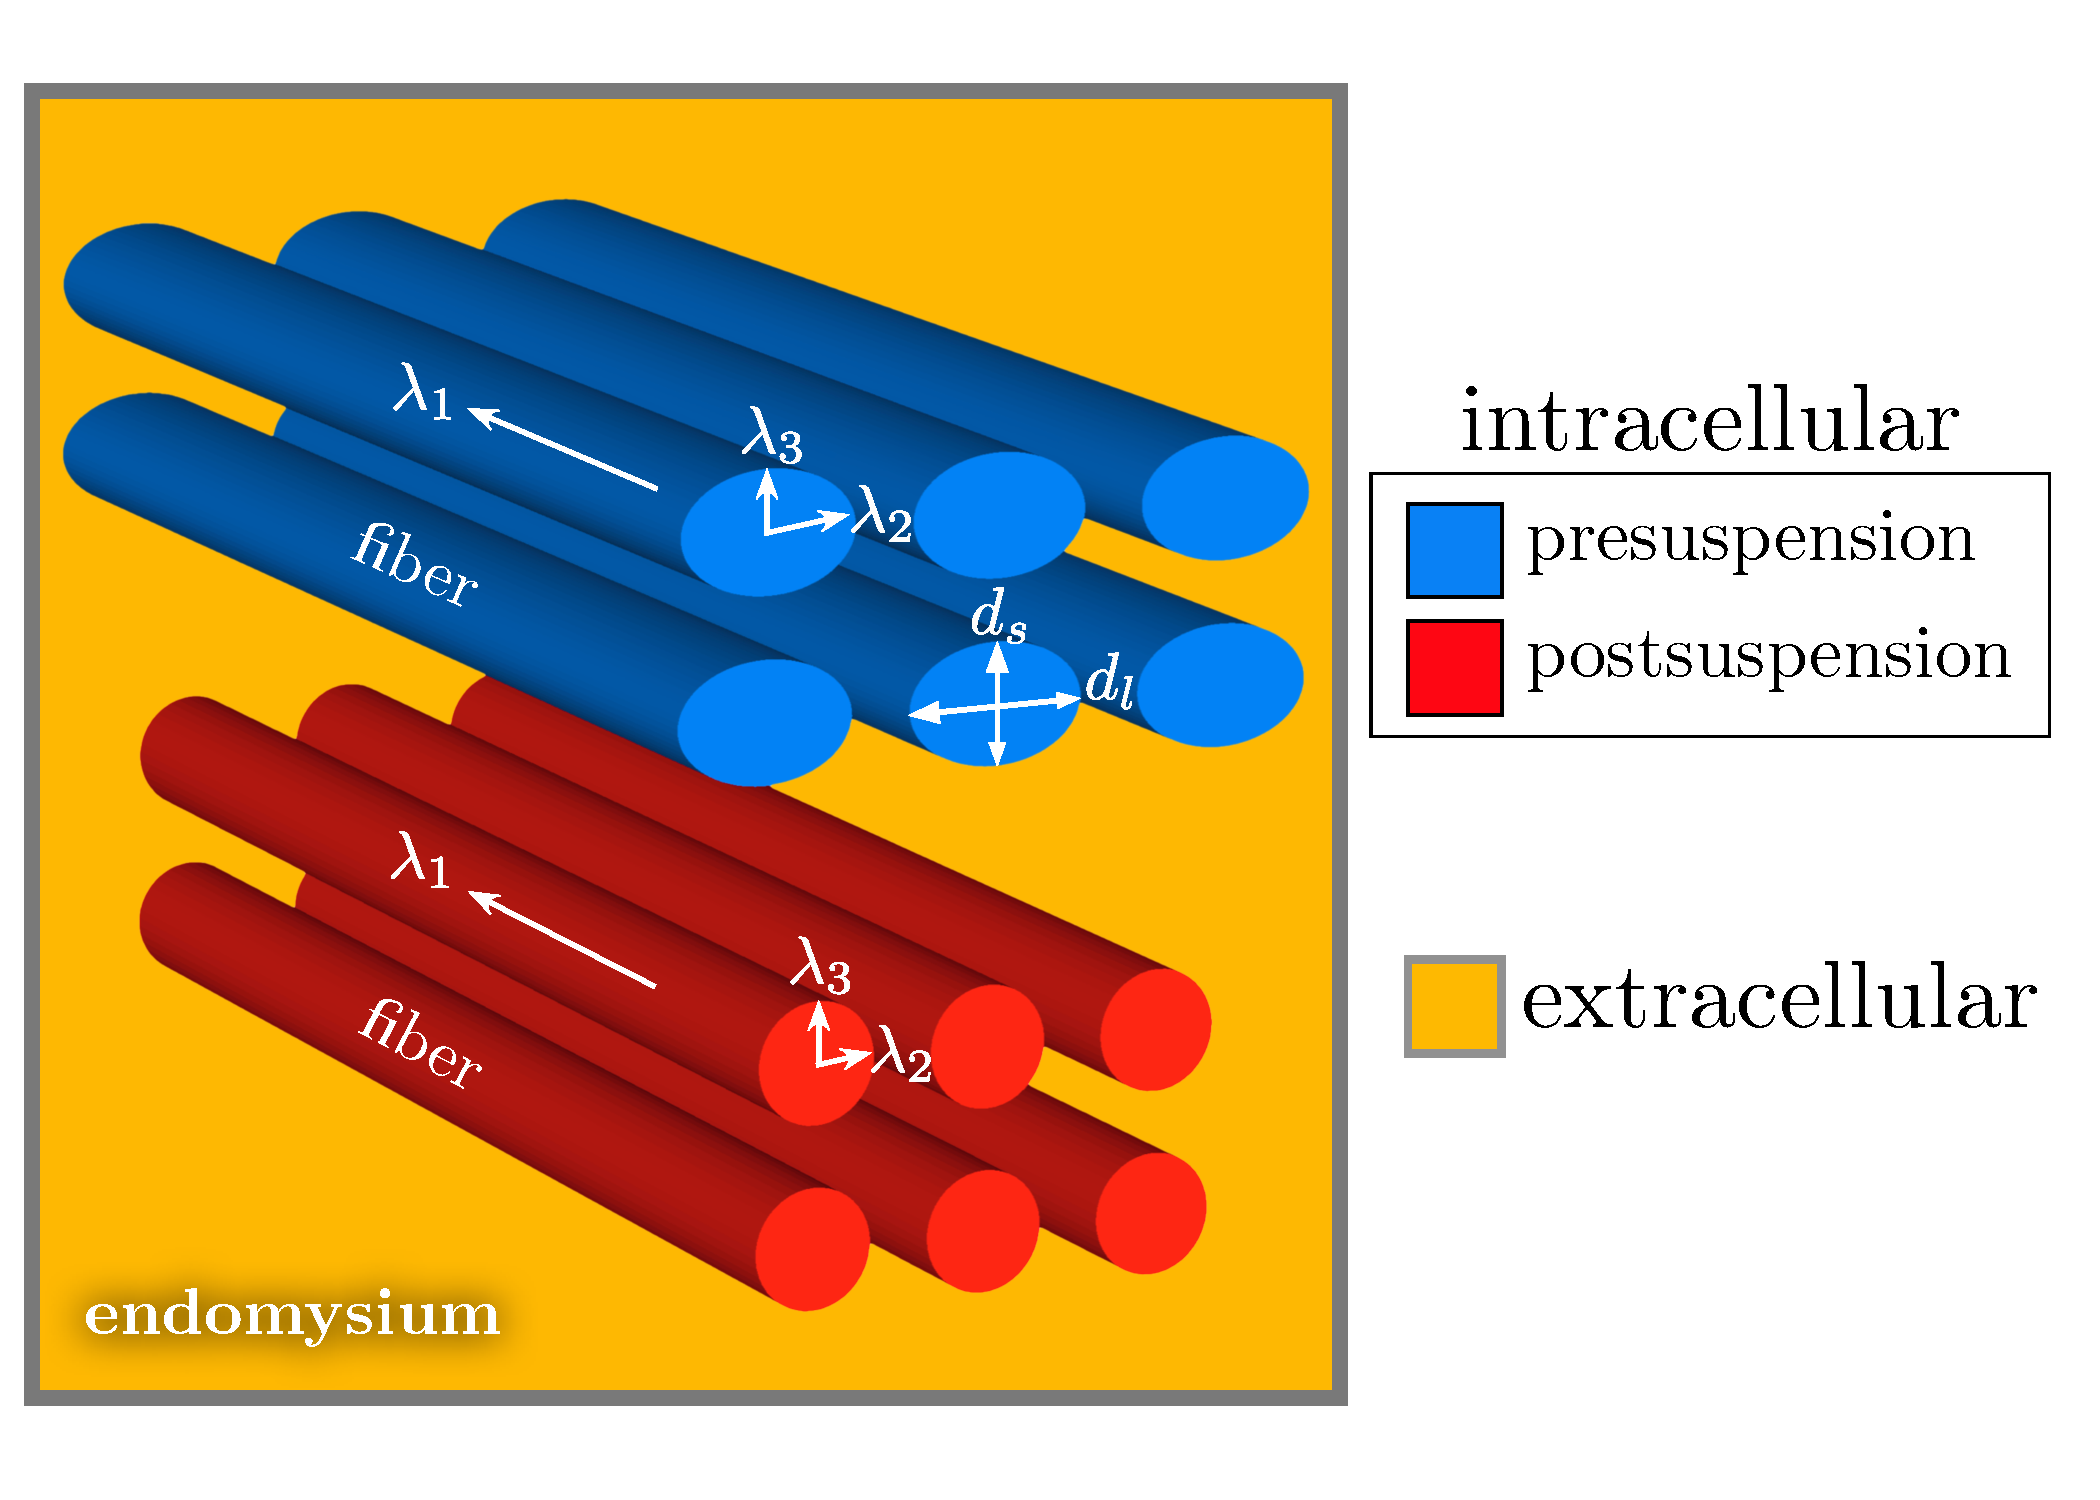
\includegraphics[scale=.3]{Figures/FibersModel.pdf}
\caption[Schematic of muscle fibers and endomaysium matrix]{Schematic of muscle fibers and endomaysium matrix.}
\label{fig: KargerModel}
\end{figure}
%*********************************************************
Muscle fiber diameter $d$ defined as the mean of the short axis and long axis lengths.
The model allows exchange between two compartments: the intracellular space (inside the muscle fiber) and the extracellular space (collagenous intramuscular connective tissue consisting of endomysium and perimysium).
The volumes of the two compartments are denoted as $\nu_{\mathrm{in}}$ (intramyocellular volume fraction) and $\nu_{\mathrm{ex}}$ (extracellular volume fraction), with $\nu_{\mathrm{in}} + \nu_{\mathrm{ex}} = 1$. 
Further, the collagen fraction in the extracellular matrix is represented by $\nu_{\mathrm{coll}}$. 
The last parameter of the fit is the intracellular residence time $(\tau_{\mathrm{in}})$, which is related to the permeability ($\kappa$) of the sarcolemma (i.e. the cell membrane of muscle fibers) through the relationship: $\tau_{\mathrm{in}} = d/2\kappa$. 
Total MR signal $S$ which is a function of time $t$ and \mbox{\textit{b-}value} is a sum of signals from intracellular and extracellular compartments:
%.........................................................
\begin{equation}\label{eq: Karger Signal}
S(t,b) = S_{\mathrm{in}}(t,b)+S_{\mathrm{ex}}(t,b)
\end{equation}
%.........................................................
Time evolution of the signals $S_\mathrm{in}$ and $S_\mathrm{ex}$ can be found from the system of ordinary differential equations:
%.........................................................
\begin{equation}\label{eq: Karger ODE}
{\setstretch{1.0}
\begin{cases}
\dfrac{dS_{\mathrm{in}}}{dt}=-q^2D^{\mathrm{app}}_{\mathrm{in}}S_{\mathrm{in}}-\dfrac{1}{\tau_{\mathrm{in}}}S_{\mathrm{in}}+\dfrac{1}{\tau_{\mathrm{ex}}}S_{\mathrm{ex}}-\dfrac{1}{\mathrm{T}_{2,\mathrm{in}}}S_{\mathrm{in}}\\[20pt]
\dfrac{dS_{\mathrm{ex}}}{dt}=-q^2D^{\mathrm{app}}_{\mathrm{ex}}S_{\mathrm{ex}}-\dfrac{1}{\tau_{\mathrm{ex}}}S_{\mathrm{ex}}+\dfrac{1}{\tau_{\mathrm{in}}}S_{\mathrm{in}}-\dfrac{1}{\mathrm{T}_{2,\mathrm{ex}}}S_{\mathrm{ex}}
\end{cases}
}
\end{equation}
%.........................................................
where $q$ is a product of gyromagnetic ratio $\gamma$, gradient $G$ of duration $\delta$. 
Using $q$ the \mbox{\textit{b-}value} can be expressed as $b=q^2(\Delta-\delta/3)$, $\Delta$ is time separation between diffusion gradients. 
With initial conditions:
%.........................................................
\begin{equation}\label{eq: Karger IC}
{\setstretch{1.0}
\begin{aligned}
& S_{\mathrm{in}}(0,b)=\nu_{\mathrm{in}}\\[10pt]
& S_{\mathrm{ex}}(0,b)=\nu_{\mathrm{ex}}\\[10pt]
& \dfrac{S_{\mathrm{in}}(0,b)}{\tau_{\mathrm{in}}}=\dfrac{S_{\mathrm{ex}}(0,b)}{\tau_{\mathrm{ex}}}
\end{aligned}
}
\end{equation}
%.........................................................
system of Equations~\ref{eq: Karger ODE} has the solution:
%.........................................................
\begin{equation}\label{eq: Karger Solution}
S(t,b)=\nu'_{\mathrm{in}} e^{-q^2tD'_{\mathrm{in}}}+\nu'_{\mathrm{ex}} e^{-q^2tD'_{\mathrm{ex}}}
\end{equation}
%.........................................................
with modified volumes and diffusion coefficients:
%.........................................................
\begin{equation}\label{eq: Karger v modified}
\begin{array}{l}
\nu'_{\mathrm{ex}} = \dfrac{1}{D'_{\mathrm{ex}}-D'_{\mathrm{in}}} \left[\nu_{\mathrm{in}}\left( D^{\mathrm{app}}_{\mathrm{in}} + \dfrac{1}{q^2 \mathrm{T}_{2,\mathrm{in}}} \right) + \nu_{\mathrm{in}}\left( D^{\mathrm{app}}_{\mathrm{in}} + \dfrac{1}{q^2 \mathrm{T}_{2,\mathrm{in}}} \right) - D'_{\mathrm{in}} \right]\\[10pt]
\nu'_{\mathrm{in}} = 1 - \nu'_{\mathrm{ex}}
\end{array}
\end{equation}
%.........................................................
%.........................................................
\begin{equation}\label{eq: Karger ADC}
\begin{split}
D'_\mathrm{in,ex} &= \frac{1}{2}\left( D^{\mathrm{app}}_\mathrm{in} + D^{\mathrm{app}}_\mathrm{ex} + \frac{1}{q^2}\left(\frac{1}{\tau_{\mathrm{in}}} + \frac{1}{\tau_{\mathrm{ex}}} + \frac{1}{\mathrm{T}_{2,\mathrm{in}}} + \frac{1}{\mathrm{T}_{2,\mathrm{ex}}} \right) \right) \mp \\ &\mp \frac{1}{2}\sqrt{\left( D^{\mathrm{app}}_\mathrm{in} - D^{\mathrm{app}}_\mathrm{ex} + \frac{1}{q^2}\left(\frac{1}{\tau_{\mathrm{in}}} - \frac{1}{\tau_{\mathrm{ex}}} - \frac{1}{\mathrm{T}_{2,\mathrm{in}}} + \frac{1}{\mathrm{T}_{2,\mathrm{ex}}} \right) \right) + \frac{4}{q^4\tau_{\mathrm{in}}\tau_{\mathrm{ex}}}}\\
\end{split}
\end{equation}
%.........................................................
\\
Intracellular apparent diffusion coefficient $D^{\mathrm{app}}_\mathrm{in}$ is found by investigating signal attenuation due to diffusion inside two impermeable walls separated by distance $d$ with gradient $G$ applied perpendicular to these walls. 
Signal $S$ defined as ratio between $\bar{M}$ and $M_{0}$ expressed through conditional probability $P(z_2|z_1, \Delta)$:
%.........................................................
\begin{equation}\label{eq: Karger AppEx}
S (t,b)= \dfrac{1}{d}\iint dz_1 dz_2  \cos \left[ \gamma \delta G (z_2-z_1)\right]P(z_2|z_1, \Delta)
\end{equation}
%.........................................................
from Fick's law (Equation~\ref{eq:probability_diffusion}) with initial conditions imposed:
%.........................................................
\begin{equation}\label{eq: probability initial conditions}
\begin{array}{c}
	P\left( z,0\right) = \delta\left( z-z_1\right)\\[10pt]
	\left. \dfrac{\partial P}{\partial z}\right\vert_{z=\pm d/2} = 0
\end{array}
\end{equation}
%.........................................................
using Equation~\ref{eq: Diffusion from bvalue} intracellular apparent diffusion coefficient is expressed:
%.........................................................
\begin{equation}\label{eq: Karger AppEx}
\begin{split}
	D^{\mathrm{app}}_{\mathrm{in}} (D_{\mathrm{in}},\Delta, b, d) &= -\dfrac{1}{b} \ln  \left[ \frac{2 - 2 \cos(qd)}{(qd)^2} + \vphantom{ \exp \left( - \frac{n^2 \pi^2 D_{\mathrm{in}} \Delta}{d^2}\right)\frac{1-(-1)^n \cos{(qd)}}{\left( \left(qd\right)^2 - \left( n \pi\right)^2\right)^2}} \right. \\
                   &+ \left. 4(qd)^2 \sum^{\infty}_{n=1} \exp \left( - \frac{n^2 \pi^2 D_{\mathrm{in}} \Delta}{d^2}\right)\frac{1-(-1)^n \cos{(qd)}}{\left( \left(qd\right)^2 - \left( n \pi\right)^2\right)^2} \right]
\end{split}
\end{equation}
%.........................................................
Extracellular apparent diffusion coefficient as a function of water diffusion coefficient $(D_{\mathrm{w}})$, orientation parameter $(\zeta)$, extracellular $(\nu_{\mathrm{ex}})$ and collagen $(\nu_{\mathrm{col}})$ volume fractions was defined in~\cite{RND12}:
%.........................................................
\begin{equation}\label{eq: Karger AppEx}
D^{\mathrm{app}}_{\mathrm{ex}}=D_{\mathrm{w}}(1-\nu_{\mathrm{col}})^{2/3}\nu_{\mathrm{ex}}^\zeta
\end{equation}
%.........................................................
where $\zeta$ can take three values: 0 when considering diffusion parallel to the longitudinal axes of cylinder, $\alpha$ when parallel to the major axis in the cylinder cross-section and $1/\alpha$ when parallel to the minor axis.
%~~~~~~~~~~~~~~~~~~~~~~~~~~~~~~~~~~~~~~~~~~~~~~~~~~~~~~~~~
\subsection{Results}
%~~~~~~~~~~~~~~~~~~~~~~~~~~~~~~~~~~~~~~~~~~~~~~~~~~~~~~~~~
Muscle force decreased significantly post-suspension (change of $-32.6 \pm 24.7\%$; $p=0.013$); this is the average over the seven subjects. 
The average change (over all subjects) in the volume of the MG, LG, and SOL muscles after the 4-week suspension was $-9.6 \pm 4.5\%$ ($p=0.001$), $-11.1 \pm 7.4\%$ ($p=0.008$), and $-7.4 \pm 5.9\%$ ($p=0.006$) respectively (significance of pre- and post- suspension volume changes indicated for each muscle).
While the DTI measurements/modeling are focused on the MG, the measured isometric plantarflexion force is generated by the Triceps Surae muscles and thus the volume change of all three muscles are included here. 
Typical maps of the eigenvalues, ADC, FA, and CP at one anatomical location of the lower leg in one subject pre- and post-suspension are shown in Figure~\ref{fig: KargerEV}. 
The two left columns are pre-suspension and the two right columns are corresponding images from the same subjects post-suspension; 
an anatomical level close top row shows the maps pre-suspension and the bottom the maps at a corresponding anatomic location post-suspension. 
The maps are (top to bottom, column 1 and 3): ADC, $\lambda_1, \lambda_2, \lambda_3$; (top to bottom, column 2 and 4): FA, CP, lead eigenvector, mask of MG muscle with ROI superposed on the eigenvalue weighted eigenvector color map. 
Eigenvalues are in units of $\SI{}{\micro\meter^2 / \milli\second}$, the FA and CP are unitless. $\mathrm{ev}_1$ is the colormap of the eigenvector corresponding to the lead eigenvalue, $\lambda_1$. 
The colormap is the projection of the primary eigenvector following the convention: Left $\rightarrow$ Right ($x$-projection): red, Anterior $\rightarrow$ Posterior ($y$-projection): green, Superior $\rightarrow$ Inferior ($z$-projection): blue. 
The predominantly blue hue confirms the superior-inferior direction of the muscle fiber. 
The same anatomic location is shown pre- and post-suspension; 
the atrophy of the muscles is clearly seen comparing the pre- to the post-suspension images. 
The effectiveness of the fat suppression can be seen by the absence of fat artifacts (shifted subcutaneous fat) in the image.
%*********************************************************
\begin{figure}[!htb]
\vspace{+0.2cm}
\centering
\includegraphics[width=\textwidth]{Figures/DTI_2compart.pdf}
\caption[The parametric maps extracted from the diffusion tensor]{The parametric maps extracted from the diffusion tensor.}
\label{fig: KargerEV}
\end{figure}
%*********************************************************
Visual assessment of the parametric DTI maps confirms the image quality (SNR) and lack of image artifacts (good fat suppression as well as small image distortions).
%-new paragraph-%

%-new paragraph-%
The DTI indices evaluated pre- and post-suspension in the medial gastrocnemius are summarized in Table~\ref{tab: Karger1};
the values listed here are the averages for all subjects. Three eigenvalues and apparent diffusion coefficient  decreased significantly post-suspension ($\lambda_1$:  $p = 0.025$, $\lambda_2$: $p = 0.035$, $\lambda_3$: $p = 0.049$, ADC: $p = 0.029$) while FA increased and CP decreased with suspension, although the latter indices two did not show significant changes ($p = 0.239$ for FA and $p=0.763$ for CP). 
The maximum decrease was in the secondary eigenvalue that in turn resulted in a smaller difference between the secondary and tertiary eigenvalue post suspension (reflected also as a decrease in CP).
%=========================================================
\begin{table}[!htb]
\vspace{+0.2cm}
\caption[Diffusion tensor indices pre- and post-suspension]{Diffusion tensor indices pre- and post-Unilateral Limb Suspension (ULLS).}
\label{tab: Karger1}
\begin{center}
\begin{threeparttable}
\begin{tabular}{@{}llll@{}}
\toprule[1pt]\midrule[0.3pt]
  &   & Pre-ULLS    & Post-ULLS   \\ \midrule
$\lambda_1$\tnote{$\dagger$} & $\left[\SI{}{\micro\meter^2 / \milli\second}\right]$ & 2.06 $\pm$ 0.11 & 1.91 $\pm$ 0.15 \\[6pt]
$\lambda_1$\tnote{$\dagger$} & $\left[\SI{}{\micro\meter^2 / \milli\second}\right]$ & 1.44 $\pm$ 0.08 & 1.31 $\pm$ 0.11 \\[6pt]
$\lambda_3$\tnote{$\dagger$}& $\left[\SI{}{\micro\meter^2 / \milli\second}\right]$ & 1.30 $\pm$ 0.11 & 1.17 $\pm$ 0.10 \\[6pt]
ADC\tnote{$\dagger$}   	&	& 1.60 $\pm$ 0.07 & 1.47 $\pm$ 0.11 \\[6pt]
FA   					&	& 0.25 $\pm$ 0.04 & 0.27 $\pm$ 0.04 \\ \midrule[0.3pt]\bottomrule[1pt]
\end{tabular}
\begin{tablenotes}[flushleft]\footnotesize
\item[$\dagger$] significant difference between pre- and post-suspension
\end{tablenotes}
\end{threeparttable}
\end{center}
\vspace{-0.2cm}
\end{table}
%=========================================================
In addition to the average over all subjects listed in Table~\ref{tab: Karger1}, the DTI indices (eigenvalues, ADC, FA and CP) pre- and post-suspension are also plotted for each subject individually in Figure~\ref{fig: KargerPlots}. 
This was done to confirm the consistency of DTI changes with suspension across the seven subjects and hence the validity of the data.
Pre- and post- values for each subject are connected for ease of visualization of the changes in the indices with suspension. 
For most of the DTI indices the majority of subjects show the same direction of changes: e.g., six out of seven subjects show a decrease in $\lambda_1, \lambda_2$, ADC, and an increase in FA, while five out of seven subjects show a decrease in $\lambda_3$ and in CP.
%*********************************************************
\begin{figure}[!htb]
\vspace{+0.2cm}
\centering
\includegraphics[width=\textwidth]{Figures/KargerPlots.pdf}
\caption[Individual plots of the DTI indices pre- and post-suspension]{Individual plots of the DTI indices pre- and post-suspension.}
\label{fig: KargerPlots}
\end{figure}
%*********************************************************
Table~\ref{tab: Karger2} lists the model parameters obtained by the search of the parameter space for the values of ($\alpha$, $d$, $\tau_{\mathrm{in}}$, $\nu_{\mathrm{in}}$, $\nu_{\mathrm{col}}$) that yielded the lowest value of the error index~\cite{RND12}. 
The increase in the ellipticity index with disuse indicates that the fiber becomes more circular, while the decrease in muscle fiber diameter is as anticipated with atrophy. 
%~~~~~~~~~~~~~~~~~~~~~~~~~~~~~~~~~~~~~~~~~~~~~~~~~~~~~~~~~
\subsection{Discussion}
%~~~~~~~~~~~~~~~~~~~~~~~~~~~~~~~~~~~~~~~~~~~~~~~~~~~~~~~~~
While it is known that the quadriceps muscles show greater atrophy than the medial gastrocnemius in aging and are a better correlate to physical function~\cite{RND27}, the motivation for the focus on the MG in the current study is based on the ease of performing functional MRI studies on the MG for correlation to structural MRI studies~\cite{RNSS4, RNCS4, Malis:2018fr, RNS16}. 
Further, calf circumference (and by extension calf muscle mass as well) has been shown in a large-scale study to provide information on muscle related disability and physical function~\cite{RND30}.
%-new paragraph-%

%-new paragraph-%
Muscle force loss was approximately greater by a factor of 3 compared to reduction in muscle mass. 
Prior work on gravitational unloading effects on fast and slow rat hind-limb muscles data indicate that predominantly slow muscles are more responsive to unloading than predominantly fast muscles~\cite{RND31}.
Since the soleus has a higher proportion of slow twitch muscles compared to the gastrocnemius muscles, it would be anticipated that the soleus would show the highest atrophy (volume decrease). 
However, comparing \% volume changes in the three muscles in the current study, larger changes were seen in the gastrocnemius muscles.  
It should be noted though that the soleus muscle had the highest changes in terms of absolute volume changes comparing pre- and post-suspension muscles.
%-new paragraph-%

%-new paragraph-%
Comparing the values of DTI indices in the current study with that reported by Karampinos~et~al.~\cite{RND12}, there are considerable differences in FA and in CP between the two studies.
The reasons for these differences may arise from differences in the measurement methodology.
A simulated echo EPI diffusion weighted sequence was used by Karampinos~et~al.~\cite{RND12} in contrast to the current study that uses a spin echo EPI diffusion weighted sequence.
It has been shown earlier that the simulated echo is better for diffusion imaging of muscle than a spin echo~\cite{RND32}. 
However, the sequence used in~\cite{RND12} has a TE of $\SI{52}{\milli\second}$~\cite{RND12} which is really long for a stimulated echo that has half the signal of a spin echo with a similar TE.
This raises the issue that the SNR of the sequence used in~\cite{RND12} may not have been high and low SNR has been shown to bias the estimation of DTI indices~\cite{RND33}.
Further, values reported for the eigenvalues and FA for the MG are in good agreement between the current study with another recent rigorous study that evaluated DTI indices for voxels with SNR $> 20$~\cite{RND33}.
%-new paragraph-%

%-new paragraph-%
Previous studies on denervation induced atrophy on rodent models showed a reduction in $\lambda_2$ and $\lambda_3$, an increase in fractional anisotropy while $\lambda_1$ was unchanged~\cite{RND8}. 
It is well accepted that DTI measurements in muscle reflect water diffusion in the intracellular space, thus the authors of this paper attributed the decrease in the secondary and tertiary eigenvalues to a decrease in the diameter of myofibers (i.e., myofiber atrophy). 
In another study, the triceps surae was assessed with DTI after Achilles tenotomy in rats~\cite{RND9}. 
Both muscle atrophy as well as a decrease in plantarflexion force was seen post-tenotomy. 
Significant decreases in $\lambda_1$, $\lambda_2$, and $\lambda_3$ and an increase in FA were seen between the control and treatment sides at four weeks post-tenotomy~\cite{RND9}. 
This is in contrast to denervation induced atrophy where no changes were seen in $\lambda_1$.
In the present study, decreases in all three eigenvalues were significant. 
The eigenvector corresponding to the lead eigenvalue is in the direction of the muscle fiber and thus $\lambda_1$ represents diffusion along the long axis of the muscle fiber. 
Since the muscle fiber is orders of magnitude greater than the diffusion distances, changes in muscle fiber length are not expected to cause changes in $\lambda_1$. 
Further, changes in fiber cross-section diameters should also not affect $\lambda_1$ as the diffusion direction is along the long axis of the muscle fiber. 
Thus, the decrease in $\lambda_1$ is difficult to explain. 
Possibly, the reduced diffusivity along the fibers' long axis is related to a loss in myosin content~\cite{RNS10} and reduction in the packing density of actin filament proteins~\cite{RND35} that result in structurally weakened sarcomeres. 
While the underlying physiological mechanisms are unclear, presented observations of a decrease in $\lambda_1$ is similar to that seen in the tenotomy induced atrophy~\cite{RND9}.
The decrease in $\lambda_2$ and $\lambda_3$ can potentially be related to a change in muscle fiber diameter and is similar to that seen in denervation induced atrophy~\cite{RND8}. 
It should also be noted that the largest decrease was seen in $\lambda_2$. 
If the secondary and tertiary eigenvalues reflect the long axis and short axis diameters respectively of the muscle fiber cross-section, then the muscle fiber is more circular post-suspension. 
%-new paragraph-%

%-new paragraph-%
In this context, Karampinos~et~al.~\cite{RND12} advanced the hypothesis that the elliptic fiber cross-section arises from a response to the mechanical stimulus as the fiber is strained more along one direction in the muscle fiber cross-section than in the orthogonal direction. 
When the mechanical stimulus is reduced or removed as with ULLS induced disuse, the preferential deformation along one axis in the fiber cross-section is removed.
This may well result in the fiber cross-section becoming more circular in the absence of a mechanical stimulus.
As opposed to the progressive circularity accompanying disuse-atrophy~\cite{RND36},
ADC decreased significantly with suspension and may potentially arise from a combination of a decrease in inherent intracellular diffusivity (decrease in all three eigenvalues) and a decrease in muscle fiber size (decrease in secondary and tertiary eigenvalues).
In the context of a reduction of a mechanical stimulus with suspension, the discussion of findings from related studies using strain/strain rate tensor imaging is worthwhile~\cite{RNSS4, RNCS4, Malis:2018fr, RNS16}. 
Strain and strain rate tensor imaging evaluate tissue deformation and the tensor provides information of the strain (or strain rate) in three orthogonal directions. 
The primary, secondary, and tertiary eigenvectors of the strain rate tensor correspond approximately to the muscle fiber direction and to two orthogonal directions in the muscle fiber cross-section, respectively. 
When the muscle fiber contracts, a negative strain will be seen along the muscle fiber direction and accompanying this, a positive strain from radial expansion will be seen in the fiber cross-section.
However, this positive strain is not symmetric in the fiber cross-section, with much larger expansion along one direction than the orthogonal direction; this asymmetry has been reported in a number of studies~\cite{Malis:2018fr, RNS16, RNS31}.
%-new paragraph-%

%-new paragraph-%
A recent study on strain rate tensor imaging after unilateral limb suspension reported that the fiber cross-section strain rate asymmetry decreased post-suspension~\cite{Malis:2018fr}.
This decrease in strain rate asymmetry may also be tied to the structural response to the lack of mechanical stimulus.
This potentially may imply that the long axis of the elliptical cross-section (proportional to the secondary eigenvalue of the diffusion tensor) is a consequence of the external mechanical stimulus since the radial expansion is preferentially along this direction resulting in an elongation of the fiber cross-section in one direction. Once this stimulus is removed (as in limb suspension) the elongated axes is no longer preferentially stretched, and may potentially become less elliptical (more circular).
This is reflected in a lower CP value post-suspension. 
Another potential explanation for the observed structural changes may be the altered muscle fiber-extracellular matrix interactions from limb suspension~\cite{RNSS4, RNCS4}. 
%-new paragraph-%

%-new paragraph-%
The values of $\alpha$ reported in the literature for the vastus lateralis muscle are in the range of $0.4$ to $0.68$~\cite{RND38, RND39}; the current value of $0.55$ for MG ellipticity in the pre-suspension case appears to be reasonable~\cite{RND38, RND39}.
Karampinos~et~al. report the value of $\alpha$ from the fit to the diffusion model with a range of $0.6 - 0.9$; the lower end of this range is close to the current paper.
The MG muscle fiber diameter extracted from the model in the current study ($\SI{82}{\micro\meter}$) is in agreement with values reported in the literature~\cite{RND38} and also with the range ($70 - \SI{110}{\micro\meter}$) determined for the MG in the earlier diffusion modeling study by Karampinos~et~al.~\cite{RND12}.
Further, the focus of the modeling was on determining if meaningful changes in microstructure with suspension can be extracted from the experimentally determined diffusion eigenvalues.
With suspension, the ratio of the short axis to long axis muscle fiber length increases which implies that the fiber becomes more circular.
In the light of the hypothesis that the elliptical muscle fiber shape arises from the mechanical stimulus, the modeling result of a more circular muscle fiber can be explained by the lack of mechanical stimulus during the 4-week suspension.
The diameter of the muscle fiber decreases; this finding is consistent with muscle fiber atrophy. 
In fitting both pre- and post-suspension DTI data, the search algorithm converged on the upper or lower limits for $\tau_{\mathrm{in}}, \nu_{\mathrm{in}}$ and $\nu_{\mathrm{col}}$.
Thus, the best-fit values for these parameters may be in error. 
The NRMSE was quite flat with respect to these variables; this was noted for $\tau_{\mathrm{in}}$ by Karampinos~et~al.~\cite{RND12}, and thus, fitting the available DTI data to this model does not allow one to draw conclusions regarding $\tau_{\mathrm{in}}, \nu_{\mathrm{in}}$ and $\nu_{\mathrm{col}}$.
%-new paragraph-%

%-new paragraph-%
There are limitations to the current study: the study population is small but since it is a longitudinal study (pre- and post-ULLS), statistical significance was reached for the changes in the eigenvalues. 
A one-point diffusion measurement is not ideal for extracting tissue parameters through modeling; future work using multi-point DTI data (obtained for example, by varying diffusion time and/or \mbox{\textit{b-}value}s) will allow more robust modeling to extract accurate values for these microstructural features. 
Further, multi-point DTI data may allow greater flexibility to extend to single subject rather than limit to cohort modeling as in the current study.
It should also be noted that if the fit was performed independently on each subject, it would have allowed testing of the significant changes in the microstructural parameters with limb suspension.
Measurements on the contralateral leg would have provided information on the effects of a change in mechanical loading of the unsuspended leg.
However, the current study was part of a larger protocol that besides DTI, included quantification of fat, connective tissue as well as functional measurements and acquiring data on the contralateral leg would have prolonged the scanning time excessively.
Further, imaging both legs at the same time was restricted by the customized coil that accommodated only one leg.
However, the customized coil provided higher SNR than vendor coils and allowed the acquisition of the entire lower leg without repositioning the subject.
%~~~~~~~~~~~~~~~~~~~~~~~~~~~~~~~~~~~~~~~~~~~~~~~~~~~~~~~~~
\subsection{Conclusion}
%~~~~~~~~~~~~~~~~~~~~~~~~~~~~~~~~~~~~~~~~~~~~~~~~~~~~~~~~~
The current study shows that the DTI eigenvalues decrease with suspension induced disuse atrophy. 
Experimentally, the secondary eigenvalue showed the largest decrease with suspension.
This could potentially be related to a hypothesis that attributes the elliptical shape of the muscle fiber cross-section as arising from a response to an external load~\cite{RND12}. 
While it is still a conjecture, the asymmetry of deformation in the fiber cross-section may result in one axis becoming longer than the orthogonal one and then unloading conditions can cause this shape asymmetry to be reduced. 
As the secondary and tertiary eigenvalues are related to the fiber cross-section diameters, this results in larger changes in the secondary eigenvalue as the fiber reduces the most in diameter along this direction with unloading. 
An exploratory modeling of the DTI data to extract microstructural parameters showed that it is feasible and the disuse atrophy related changes in muscle ellipticity, mean diameter, residence time, intracellular volume and collagen volume extracted from the model were physiologically reasonable.
%=========================================================
\section{Random Permeable Barrier Modeling of Age Induced Changes in the Time Dependent Diffusion Eigenvalues}
\label{sec: STEAM RPBM}
%=========================================================
Muscle mass loss have been reported in the aging muscle and this is in part, responsible for functional loss. 
However, non-invasive monitoring of microstructural changes as in muscle fiber diameter with age has not been reported. 
Commonly employed diffusion weighted acquisition protocols collect data at a single diffusion time. 
The time dependence of the diffusion tensor eigenvalues can provide additional information to improve quantification of tissue microstructure. 
A diffusion model is required to make inferences about the microstructure from the time dependent eigenvalue data.
Random permeability barrier model (RPBM) was recently introduced and applied to retrieve microscopic parameters such as membrane permeability and fiber diameter in human skeletal muscles~\cite{NovikovRPBM, RND13}. 
%~~~~~~~~~~~~~~~~~~~~~~~~~~~~~~~~~~~~~~~~~~~~~~~~~~~~~~~~~
\subsection{Random Permeable Barrier Model}
%~~~~~~~~~~~~~~~~~~~~~~~~~~~~~~~~~~~~~~~~~~~~~~~~~~~~~~~~~
The model treats muscle as a volume with randomly oriented infinite flat semipermeable membranes. 
For each membrane permeability ($\kappa$) relates the difference in concentrations on both sides of the membrane and the flux through it which provides the following boundary conditions:
%.........................................................
\begin{equation}\label{eq: RPBM bc}
D_0\mathbf{n}\left.\frac{\partial{c}}{\partial r} \right\vert_{\pm} = \kappa \left[ c|_+ - c|_-  \right]
\end{equation}
%.........................................................
RPBM model is characterized by three parameters: the free diffusion coefficient ($D_0$), membrane surface to volume ratio ($S/V$) and permeability ($\kappa$). Time-dependent diffusion coefficient is found by solving the diffusion equation (Equation~\ref{eq:Fick2}) and then averaging the result over disorder using real-space renormalization group~\cite{NovikovRPBM}.
%.........................................................
\begin{equation}\label{eq: RPBM}
D(t) = \frac{D_0}{2\pi t}\int\limits^{\infty}_{-\infty}\dfrac{d\omega}{(-i\omega)^2}\frac{e^{-i\omega t}}{1 + \zeta +2z_{\omega}(1-z_{\omega})  \left[\sqrt{1+\zeta/\left(1-z_{\omega}\right)}-1 \right] }
\end{equation}
%.........................................................
where $z_\omega = i \sqrt{i \omega t}$ and $\zeta=(S/V)D_0/4\kappa$ is an effective volume fraction occupied by membranes.
The integral~(\ref{eq: RPBM bc}) can be integrated numerically as outlined in reference~\cite{RND13}.
%~~~~~~~~~~~~~~~~~~~~~~~~~~~~~~~~~~~~~~~~~~~~~~~~~~~~~~~~~
\subsection{Materials and Methods}
%~~~~~~~~~~~~~~~~~~~~~~~~~~~~~~~~~~~~~~~~~~~~~~~~~~~~~~~~~
Image acquisition protocol used a custom-built STEAM-EPI DTI sequence (Figure~\ref{fig: STEAM_GE}) discussed in more details in section~\ref{sec: EPI}. 
A water selective SPSP RF-pulse was used for fat suppression. 
Six non-collinear gradient directions with a nominal \mbox{\textit{b-}value} of $\SI{400}{\second \per\milli\meter^2}$ were used to map the direction dependent diffusion at ten values of the diffusion time~$\Delta$ ($\SI{20}{\milli\second}$ to $\SI{600}{\milli\second}$). 
Imaging parameters were: echo time (TE) $\SI{32}{\milli\second}$, repetition time (TR) $\SI{4000}{\milli\second}$, $2$ signal averages, acquisition matrix size $80 \times 80$, field of view (FOV) $200 \times 200 \; \SI{}{\milli\meter^2}$, 3 slices of $\SI{5}{\milli\meter}$ thickness. 
Diffusion data were pre-processed for eddy current mis-registration and denoised by applying Joint-Rican LMMSE filter~\cite{RND24} prior to computing the diffusion tensor and the diffusion eigenvalues. 
The corrected full \textit{b-}matrix that accounted for the diffusion, imaging and crusher gradients was calculated as outlined in subsection~\ref{subsection: STEAM b value}. For the nominal $b = 0$ images, the \mbox{\textit{b-}value} varied from $\SI{1.7}{\second \per  \milli\meter^2}$ at $\Delta = \SI{20}{\milli\second}$ to $\SI{22}{\second\per\milli\meter^2}$ at $\Delta = \SI{600}{\milli\second}$ and for the nominal $b = \SI{400}{\second\per\milli\meter^2}$ images, the \mbox{\textit{b-}value} varied from $\SI{371}{\second\per\milli\meter^2}$ at $\Delta = \SI{20}{\milli\second}$ to $\SI{547}{\second\per\milli\meter^2}$ at $\SI{600}{\milli\second}$, emphasizing the need for full \textit{b-}matrix calculation. 
Prior to human scans a set of images was obtained in a water phantom following the same imaging protocol as described above. 
Fractional anisotropy (FA) maps were calculated from the acquired data to validate diffusion tensor calculations at long diffusion times. 
FA maps side by side with the corresponding magnitude images at nominal \mbox{\textit{b-}value} for diffusion times 20 and $\SI{600}{\milli\second}$ are show in the Figure~\ref{fig:STEAM phantom}. 
%*********************************************************
\begin{figure}[!htb]
\vspace{+0.2cm}
\centering
\includegraphics[width=0.9\textwidth]{Figures/STEAM_Phantom.pdf}
\caption[Baseline magnitude images and FA colormaps of water phantom acquired with STEAM-EPI DTI image sequence at two diffusion times]{Baseline magnitude images and FA colormaps of water phantom acquired with STEAM-EPI DTI image sequence at two mixing times: 20 and $\SI{590}{\milli\second}$.}
\label{fig:STEAM phantom}
\end{figure}
%*********************************************************
%-new paragraph-%

%-new paragraph-%
All human imaging studies were performed after IRB approval on a $\SI{3}{\tesla}$ scanner (GE Medical Systems, WI, USA) on seven young ($31 \pm 8$ years) and six senior ($75 \pm 5$ years) subjects. 
The RPBM model was fitted by fixing the free diffusion coefficient $D_0$ at the long diffusion time limit of the primary eigenvalue ($\lambda_1$) to extract the following parameters: the membrane permeability ($\kappa$), and the membrane surface to volume ratio ($S/V$). 
The myofiber size (a) is derived from the surface to volume ratio as: $4V/S$. 
The RPBM fits were made to the time dependence of the average of $\lambda_2$, and $\lambda_3$ ($D_{\perp}$); the values of $D_{\perp}$ were the average over the medial gastrocnemius (MG) muscle segmented from all three~slices.
%~~~~~~~~~~~~~~~~~~~~~~~~~~~~~~~~~~~~~~~~~~~~~~~~~~~~~~~~~
\subsection{Results}
%~~~~~~~~~~~~~~~~~~~~~~~~~~~~~~~~~~~~~~~~~~~~~~~~~~~~~~~~~
Figure~\ref{fig:STEAM_EV} shows parametric $D_\parallel$ and $D_\perp$ maps for a young and for a senior subject at two diffusion times.
Excellent fat suppression was seen in all the STEAM DTI data. 
Typical eigenvalue images ($D_\parallel \equiv \lambda_1$) and ($D_\perp \equiv (\lambda_2 + \lambda_3)/2$) at two values of mixing time ($20$ and $\SI{590}{\milli\second}$) for a young (left panel) and a senior (right panel) subject. 
The decrease in SNR with diffusion time can be visualized by the noisier images of the bottom panel. 
%*********************************************************
\begin{figure}[!htb]
\vspace{+0.2cm}
\centering
\includegraphics[width=0.9\textwidth]{Figures/STEAM_EV.pdf}
\caption[Diffusion tensor eigenvalues grayscale maps at two values of mixing time  for a young and a senior subject]{Diffusion tensor eigenvalues $D_\parallel$ and $D_\perp$ grayscale maps at two values of mixing time (20 and $\SI{600}{\milli\second}$) for a young (left) and a senior (right) subject. The decrease in SNR with TM can be visualized by the noisier images of the bottom panel.}
\label{fig:STEAM_EV}
\end{figure}
%*********************************************************
%=========================================================
\begin{table}[!htb]
\vspace{+0.2cm}
\begin{center}
\caption[Diffusion eigenvalues at different mixing times]{Diffusion eigenvalues ($\lambda_1, \lambda_2, \lambda_3$) at different mixing times.}
\label{tab:RPBM}
\begin{tabular}{@{}ccccccccc@{}}
\toprule[1pt]\midrule[0.3pt]
\multirow{2}{*}{$\mathrm{TM}$ {[}ms{]}} & \multicolumn{2}{c}{$\lambda_1 \quad [\SI{}{\micro\meter^2\per\milli\second}]$}  &  & \multicolumn{2}{c}{$\lambda_2 \quad [\SI{}{\micro\meter^2\per\milli\second}]$}  &  & \multicolumn{2}{c}{$\lambda_3 \quad [\SI{}{\micro\meter^2\per\milli\second}]$}  \\ \cmidrule(lr){2-3} \cmidrule(lr){5-6} \cmidrule(lr){8-9} 
                             & Young     & Senior    &  & Young     & Senior    &  & Young     & Senior    \\ \cmidrule(){1-9}
20                           & 2.8 $\pm$ 0.2 & 2.8 $\pm$ 0.2 &  & 2.4 $\pm$ 0.1 & 2.3 $\pm$ 0.3 &  & 1.2 $\pm$ 0.1 & 1.2 $\pm$ 0.1 \\
30                           & 2.6 $\pm$ 0.2 & 2.7 $\pm$ 0.2 &  & 2.0 $\pm$ 0.1 & 2.1 $\pm$ 0.3 &  & 1.2 $\pm$ 0.1 & 1.3 $\pm$ 0.1 \\
60                           & 2.4 $\pm$ 0.2 & 2.5 $\pm$ 0.2 &  & 1.9 $\pm$ 0.2 & 1.8 $\pm$ 0.2 &  & 0.8 $\pm$ 0.1 & 1.0 $\pm$ 0.2 \\
90                           & 2.4 $\pm$ 0.3 & 2.4 $\pm$ 0.2 &  & 1.7 $\pm$ 0.2 & 1.7 $\pm$ 0.2 &  & 0.8 $\pm$ 0.1 & 0.9 $\pm$ 0.1 \\
190                          & 2.3 $\pm$ 0.3 & 2.3 $\pm$ 0.2 &  & 1.7 $\pm$ 0.1 & 1.7 $\pm$ 0.2 &  & 0.4 $\pm$ 0.1 & 0.6 $\pm$ 0.1 \\
290                          & 2.2 $\pm$ 0.2 & 2.2 $\pm$ 0.2 &  & 1.8 $\pm$ 0.1 & 1.7 $\pm$ 0.1 &  & 0.2 $\pm$ 0.1 & 0.4 $\pm$ 0.1 \\
340                          & 2.2 $\pm$ 0.1 & 2.2 $\pm$ 0.2 &  & 1.2 $\pm$ 0.1 & 1.3 $\pm$ 0.1 &  & 0.7 $\pm$ 0.1 & 0.8 $\pm$ 0.1 \\
390                          & 2.2 $\pm$ 0.1 & 2.2 $\pm$ 0.3 &  & 1.3 $\pm$ 0.2 & 1.3 $\pm$ 0.2 &  & 0.7 $\pm$ 0.1 & 0.7 $\pm$ 0.1 \\
490                          & 2.1 $\pm$ 0.1 & 2.2 $\pm$ 0.2 &  & 1.3 $\pm$ 0.2 & 1.3 $\pm$ 0.1 &  & 0.6 $\pm$ 0.1 & 0.7 $\pm$ 0.1 \\
590                          & 2.1 $\pm$ 0.2 & 2.2 $\pm$ 0.2 &  & 1.3 $\pm$ 0.2 & 1.3 $\pm$ 0.1 &  & 0.6 $\pm$ 0.1 & 0.7 $\pm$ 0.1 \\ \midrule[0.3pt]\bottomrule[1pt]
\end{tabular}
\end{center}
\vspace{-0.2cm}
\end{table}
%=========================================================
Table~\ref{tab:RPBM} summarizes the eigenvalues for the MG muscle in the young and senior cohort at the ten diffusion times. 
Larger changes with diffusion time are seen in $\lambda_2$, and $\lambda_3$ (compared~to~$\lambda_1$). 
The RPBM fits to the time dependence of $D_\perp$ for a subject from the young cohort and from the senior cohort are shown for the Figure~\ref{fig:RPBM fit}. The large variation of $D_\perp$ with TM is in contrast to the smaller variation of $D_\parallel$ with TM.
Table~\ref{tab:RPBM2} is a list of model derived muscle microstructure parameters; volume fraction decreased with age while diffusion time and residence time in a cell increased with age while other model parameters such as the fiber size and membrane permeability increased with age but did not reach significance.
%*********************************************************
\begin{figure}[!htb]
\vspace{+0.2cm}
\centering
\includegraphics[width=\textwidth]{Figures/RPBM_fit.pdf}
\caption[RPBM model fit to the time dependence of diffusion indices for a young and senior subjects]{RPBM model fit to the time dependence of diffusion indices for a young and senior subjects.}
\label{fig:RPBM fit}
\end{figure}
%*********************************************************
%=========================================================
\begin{table}[!htb]
\vspace{+0.2cm}
\begin{center}
\caption[Parameters of muscle tissue extracted from the RPBM model]{Parameters of muscle tissue extracted from the RPBM model.}
\label{tab:RPBM2}
\begin{tabular}{@{}lrr@{}}
\toprule[1pt]\midrule[0.3pt]
                        								& \multicolumn{1}{c}{Young}         & \multicolumn{1}{c}{Senior}  \\ \cmidrule(){1-3}
$D_0 \; \left[\SI{}{\micro\meter^2\per\milli\second}\right]$      & \multirow{2}{*}{2.20 $\pm$ 0.16}  & \multirow{2}{*}{2.18 $\pm$ 0.24}   \\
free diffusion          								&                                	&                                \\[6pt]
$\zeta$                 								& \multirow{2}{*}{3.26 $\pm$ 1.62}  & \multirow{2}{*}{2.79 $\pm$ 0.63}   \\
volume fraction         								&                                	&                                 \\[6pt]
$S/V \; \left[\SI{}{\micro\meter^{-1}}\right]$                      & \multirow{2}{*}{0.14 $\pm$ 0.03}  & \multirow{2}{*}{0.13 $\pm$ 0.02}   \\
surface to volume ratio 								&                                	&                                 \\[6pt]
$\kappa \; \left[\SI{}{\micro\meter / \milli\second}\right]$		& \multirow{2}{*}{0.025 $\pm$ 0.005}& \multirow{2}{*}{0.027 $\pm$ 0.009} \\
permeability            								&                                	&                                 \\[6pt]
$a \; \left[\SI{}{\micro\meter}\right]$                        	& \multirow{2}{*}{28.63 $\pm$ 4.94} & \multirow{2}{*}{32.00 $\pm$ 3.72}  \\
myofiber diameter       								&                                	&                                 \\[6pt]
$\tau_{R} \; \left[\SI{}{\milli\second}\right]$                        								& \multirow{2}{*}{552.2 $\pm$ 122.1}& \multirow{2}{*}{650.6 $\pm$ 159.2} \\
residence time  								&                                	&                                 \\[6pt]
$\tau_{D} \; \left[\SI{}{\milli\second}\right]$                       								& \multirow{2}{*}{194.5 $\pm$ 71.9} & \multirow{2}{*}{238.1 $\pm$ 50.7}  \\
diffusion time  								&                                	&                                \\ \midrule[0.3pt]\bottomrule[1pt]
\end{tabular}
\end{center}
\vspace{-0.2cm}
\end{table}
%=========================================================
%~~~~~~~~~~~~~~~~~~~~~~~~~~~~~~~~~~~~~~~~~~~~~~~~~~~~~~~~~
\subsection{Discussion} 
%~~~~~~~~~~~~~~~~~~~~~~~~~~~~~~~~~~~~~~~~~~~~~~~~~~~~~~~~~
The values of the model derived parameters are in general agreement with that reported for the MG in an earlier study. 
The RPBM model yields a lower volume fraction for the aging muscle which is a measure of the membrane's ability to hinder diffusion. 
It is possible that aging muscle may have compromised sarcolemma integrity that makes it more permeable and thus poses less of a barrier to diffusion. 
Based on the fact that muscle atrophies with age a decrease in fiber diameter with age is expected. 
However fiber diameters derived from the RPBM model did not show anticipated changes. 
A sarcolemma with compromised integrity (as seen here in aging muscle) may potentially affect lateral transmission of force, the latter is mediated by proteins in the sarcolemma.
%~~~~~~~~~~~~~~~~~~~~~~~~~~~~~~~~~~~~~~~~~~~~~~~~~~~~~~~~~
\subsection{Conclusions} 
%~~~~~~~~~~~~~~~~~~~~~~~~~~~~~~~~~~~~~~~~~~~~~~~~~~~~~~~~~
The study has demonstrated the potential of diffusion modeling to extract muscle tissue parameters from time dependent $D_\perp$ derived from DTI data and its potential application it to study age related skeletal muscle remodeling.
%~~~~~~~~~~~~~~~~~~~~~~~~~~~~~~~~~~~~~~~~~~~~~~~~~~~~~~~~~
\section{Acknowledgments}
%~~~~~~~~~~~~~~~~~~~~~~~~~~~~~~~~~~~~~~~~~~~~~~~~~~~~~~~~~
Section~\ref{sec: DTI ULLS} is a reprint of material, with additional details provided in subsection~\ref{subsec: bicompart}, as it appears in: V.~Malis, U.~Sinha, R.~Csapo, M.~Narici, E.~Smitaman, and S.~Sinha, ``Diffusion tensor imaging and diffusion modeling: Application to monitoring changes in the medial gastrocnemius in disuse atrophy induced by unilateral limb suspension,'' \emph{J. Magn. Reson. Imaging}, vol. 49, no. 6, pp. 1655-1664, Dec. 2018.
The author of the dissertation was the primary author of this paper.
%-new paragraph-%

%-new paragraph-%
Section~\ref{sec: STEAM RPBM} is a reprint of material, with additional details, as it appears in: V.~Malis, S.~Sinha, E.~Smitaman, and U.~Sinha, ``Skeletal Muscle Diffusion Modeling to Identify Age Related Remodeling of Muscle Microstructure,'' \emph{Proceedings of the International Society of Magnetic Resonance in Medicine}, Sydney, 2020.
The author of the dissertation was the primary author of this abstract.
\chapter{Conclusion: Summary of the Developed Methods and Application in Future Studies.}
This chapter is a summary of the results reported in this dissertation and the possible technical and physiology-based extensions of this work in the future. 
%-new paragraph-%

%-new paragraph-%
\textit{Functional MR imaging:} Based on the studies reported in this dissertation a new greatly expanded and improved framework for \textit{in-vivo} evaluation of human muscle dynamics was developed.
The methods presented in this work will allow assessment of detailed 3D strain /strain rate patterns in significantly reduced, of up to four times of previous, scan times.
Compressed sensing with established reconstruction and analysis pipeline enables to perform data acquisition and strain/strain rate calculations at sub-maximal forces even in senior human subjects.
The physiological findings revealed that shear strain emerged as the primary and significant predictor of both force variation in the aging study and force loss in the disuse atrophy study; the second most important predictor was the normal strain rate in the fiber cross-section. 
The significance of shear strain as an important determinant of force was seen across different analysis: 2D strain rate, 3D strain and strain rate. 
There are several notable observations based on these results: MR measured shear strain is hypothesized to be the shear of the endomysium from adjacent contracting muscle fibers and is the underlying mechanism of lateral transmission of force. 
Validation for this hypothesis comes from computational models by other research groups that explored the transmission pathways for prematurely terminating or damaged muscle fibers. 
The normal strain in the fiber cross-section is constrained by the stiffness of the surrounding matrix (i.e., the endomysium and perimysium). 
Increase in collagen increases the stiffness and the width of endomysium and is known to occur with age and possibly also, to a lesser degree with disuse. 
The changes in the normal strain may reflect the increasing stiffness of the surrounding matrix. 
The last important observation is that the normal strain in the fiber cross-section is highly asymmetric in the young healthy muscle, with deformation occurring almost entirely in the plane of the fibers. 
In disuse atrophy, this anisotropy is reduced significantly. 
Computational models have shown that a deformation constrained to one direction produces a higher force than one without such a constraint. 
This loss in asymmetry of deformation may also partially explain the force loss with unloading. 
The underlying cause for the loss in asymmetry may arise from changes in costameric proteins that link muscle fibers and ECM. 
In summary, the functional studies reported in this dissertation have identified two strain indices as novel predictors of force loss/differences. 
Both these strain indices are highly sensitive to the status of the extracellular matrix providing support to conclusions reached in recent animal studies on the role of the ECM in muscle force loss with age. 
However, conclusive proof of the link between MR measured shear strain and lateral transmission of force awaits animal studies where MR and invasive studies can be performed on the same animal. 
Further, imaging based subject specific computational models are required to verify the causal link between shear in the endomysium and the voxel-based shear strain patterns (that can be quantified by MRI).
%-new paragraph-%

%-new paragraph-%
Future studies should include further technical advances towards even more rapid scanning as well as explorations to develop a comprehensive model of muscle force loss. 
In technical work, future work will focus on achieving higher data acquisition acceleration factors integrating more incoherent patterns (e.g., randomization along the velocity dimension) and joint reconstructions and spatial three dimensional compressed sensing acquisition. 
There are also several unanswered questions in physiology that can be addressed using the technical tools developed in the dissertation. 
Immediate future efforts will be focused on validation studies of the strain indices by animal studies and computational modeling. 
Other physiological studies will include extension to disease states such as muscular dystrophy, longitudinal monitoring of exercise regimens and computation of single muscle force.
%-new paragraph-%

%-new paragraph-%
\textit{Diffusion tensor imaging and modeling:} The study presented in chapter~\ref{ch: DiffusionExp} has demonstrated that diffusion models can relate changes observed at the voxel level to changes in the tissue microarchitecture
The two-compartment model applied to DTI data pre- and post-suspension showed that muscle fiber, permeability and intracellular volume decreased and collagen increased while muscle ellipticity decreased post-suspension; the latter could potentially be explained by the lack of a mechanical stimulus during unloading. 
The RPBM was applied to time dependent DTI data on old and young cohorts.
Model derived volume fraction (measure of the membrane's ability to hinder diffusion) decreased with age while diffusion time and residence time in a cell increased with age while other model parameters such as the free diffusion coefficient, the fiber size, and membrane permeability did not.
Modeling can be further improved by limiting the range for the parameters used in the fit.
This can be achieved by acquiring additional data with another imaging techniques such as Ultra-low TE (TE) and quantitative Magnetization Transfer (qMT).
Diffusion model-derived parameters can be used to generate subject specific computational models allowing predictions of force and strain distributions; the models in turn can be validated using the functional MR data.
%-new paragraph-%

%-new paragraph-%
Future work in diffusion tensor imaging will focus on technical developments including sequence development (e.g., Q-ball imaging, multi-shell imaging) as well as extensions to the currently proposed muscle diffusion models. 
On-going work in our group includes validation of the fiber diameters and permeability from the DTI model to corresponding values determined from biopsy of muscle tissue on the same subject. 
The reference values from the biopsy analysis will be used to fine tune the DTI model. 
The physiological applications of DTI modeling extend from monitoring structural changes in normal aging, longitudinal monitoring of interventions to tracking disease progress.
%-new paragraph-%

%-new paragraph-%
The functional and structural MR imaging reported in this dissertation are part of a bigger goal in Prof. Sinha's group: to develop MR techniques for comprehensive assessment of muscle with a focus on the extracellular matrix.
 These imaging biomarkers, once established, will be able to advance the diagnosis, tracking of natural progression, and response to therapy in different musculoskeletal conditions ranging from sarcopenia, disuse atrophy to dystrophies. 
\hyphenation{CS-factor}
\hyphenation{k-space}
\hyphenation{b-value}

%% APPENDIX
\appendix
\chapter{Institutional Review Board Approval}
A copy of the original IRB review and approval letter that granted permission for the experiments.
\includepdf[pages=-,scale=0.85,offset=0 0,pagecommand={}]{IRB.pdf}
%Anova



%% END MATTER
% \printindex %% Uncomment to display the index
% \nocite{}  %% Put any references that you want to include in the bib 
%               but haven't cited in the braces.
\bibliographystyle{ieeetr}
%\bibliographystyle{unsrt}
%% This is just my personal favorite style. 
%                              There are many others.
%\setlength{\bibleftmargin}{0.25in}  % indent each item
%\setlength{\bibindent}{-\bibleftmargin}  % unindent the first line
%\def\baselinestretch{1.0}  % force single spacing
%\setlength{\bibitemsep}{0.16in}  % add extra space between items
\bibliography{template}  %% This looks for the bibliography in template.bib 
%                          which should be formatted as a bibtex file.
%                          and needs to be separately compiled into a bbl file.
\singlespace  %to force bibilography environment to use single spacing for each entry 
              %double spacing between entries remains
\end{document}
